%% makeindex these0.nlo -s nomencl.ist -o these0.nls -t these0.nlg
%!TEX spellcheck = en_US
%!TEX root = thesis.tex

\documentclass[11pt, twoside, openright]{thesis}

% --------------------------------------
% Packages

\addbibresource{add.bib}
\addbibresource{cryptobib/abbrev0.bib}
\addbibresource{cryptobib/crypto.bib}
\usepackage{psl-cover}
\usepackage{lmodern}
\usepackage{appendix}

\usepackage{amssymb}
\usepackage{amsmath}
\usepackage{amsthm}

\usepackage{comment} % for commenting large sections of text

\usepackage{todonotes}

\usepackage{ifthen}
\usepackage{tikz}
\usepackage{xstring}
\usepackage[rgb]{xcolor}
\usepackage{xparse} % for double default arguments in macros
\usetikzlibrary{arrows.meta, positioning, fit, calc, patterns, patterns.meta, matrix, decorations.pathreplacing, backgrounds}

\usepackage{enumitem}
\usepackage[algo2e]{algorithm2e} % for algorithms
\usepackage{algorithm}
\usepackage{algpseudocode}
\algnewcommand{\LineComment}[1]{\State{\color{gray} \(\triangleright\) #1}}
\usepackage{listings}
\usepackage{graphicx}
\usepackage{caption}  % for \captionof if needed
\usepackage{subcaption}
\usepackage{float}    % optional, for [H] positioning

\usepackage{adjustbox}	% for table in Hippogryph
\usepackage{mathtools}	% for \vcentcolon
\usepackage{stmaryrd} % Where \llbracket and \rrbracket are defined
\usepackage{csquotes} 	% to silence warning
\usepackage{xparse} % for NewDocumentCommand	

	
% --------------------------------------

\definecolor{maincolor}{RGB}{36, 56, 141}
\colorlet{secondarycolor}{violet}

%%%==============================
\title{Développement d'Opérations Optimisées pour la Cryptographie Homomorphe}

\institute{l’École Normale Supérieure de Paris}
\doctoralschool{Sciences Mathématiques de\\ Paris Centre}{386}
\specialty{Informatique}

\author{Nicolas Bon}
\date{TBC}
\jurymember{1}{Caroline FONTAINE}{Université Paris-Saclay}{Rapportrice}
\jurymember{2}{Pierre-Alain FOUQUE}{Université Rennes 1}{Rapporteur}
\jurymember{3}{Ilaria CHILLOTTI}{Desilo}{Examinatrice}
\jurymember{4}{Adeline ROUX-LANGLOIS}{Normandie Université}{Examinatrice}
\jurymember{5}{Renaud SIRDEY}{Commissariat à l'Energie Atomique}{Examinateur}
\jurymember{6}{David POINTCHEVAL}{Ecole Normale Supérieure}{Directeur de thèse}
\jurymember{7}{Sonia BELAÏD}{CryptoExperts}{Coencadrante de thèse}
\jurymember{8}{Matthieu RIVAIN}{CryptoExperts}{Codirecteur de thèse}

% Abstract/Résumé/Mots-clés/Keywords
\frabstract{
%Résumé
}
\enabstract{
%Abstract
\vfill
}
\frkeywords{Mots-Clés {\Large\color{maincolor}$\star$} }
\enkeywords{Keywords {\Large\color{maincolor}$\star$} }

%%%==============================
\begin{document}
\frontmatter 
\hypersetup{pageanchor=false}
\maketitle
\hypersetup{pageanchor=true}
\dominitoc

 \begin{dedication}
   Dedication...
 \end{dedication}

% =============================================
%                 BEGIN
% =============================================

\cleardoublepage
\chapter*{Résumé}
\addstarredchapter{Résumé}
\thefrabstract{
	Dans cette thèse, nous étudions le chiffrement homomorphe, une technique cryptographique qui permet d’effectuer des calculs directement sur des données chiffrées, sans nécessiter de déchiffrement préalable. Ce domaine a connu un essor spectaculaire au cours des quinze dernières années, avec l’émergence de nombreux schémas de chiffrement de plus en plus performants. Néanmoins, les calculs homomorphes restent encore nettement plus coûteux que leurs équivalents classiques, ce qui freine leur adoption dans des applications concrètes.
	
	Nous nous concentrons dans ce travail sur l’un des schémas les plus prometteurs : TFHE. Nous proposons de nouvelles techniques destinées à accélérer les calculs homomorphes pour différents cas d’usage. En exploitant un encodage innovant des messages, nous commençons par convevoir des algorithmes plus efficaces pour l’évaluation homomorphe de fonctions booléennes.
	
	Dans un second temps, nous abordons le problème du transchiffrement, une approche visant à réduire la consommation de bande passante lors de la transmission de données chiffrées de manière homomorphe. Cela nécessite l’évaluation d’un algorithme de chiffrement symétrique dans le domaine homomorphe. Pour cela, et toujours en nous appuyant sur notre technique d’encodage, nous développons une implémentation homomorphe du chiffrement standard AES, plus rapide que celles de l’état de l’art, et contribuons à la conception d’un chiffrement par flot spécifiquement optimisé pour le transchiffrement.
	
	Nous poursuivons avec une contribution qui étend les capacités de TFHE, en lui permettant de fonctionner sur des espaces de messages plus larges. Cette amélioration est possible grâce à un nouvel algorithme d’évaluation de table de correspondances dans ces espaces étendus.
	
	Enfin, nous proposons une méthode conceptuellement simple et pratique pour générer des jeux de paramètres assurant sécurité, exactitude des calculs et efficacité, facilitant ainsi l’usage de TFHE dans les applications concrètes.
}
\vfill
\thefrkeywords{Cryptographie, Chiffrement complètement homomorphe, Calcul sécurisé}
\cleardoublepage
\chapter*{Abstract}
\addstarredchapter{Abstract}
\theenabstract{
	In this thesis, we study fully homomorphic encryption, a cryptographic technique that allows computations to be performed directly on encrypted data, without requiring prior decryption. This field has experienced remarkable growth over the past fifteen years, with the emergence of increasingly efficient encryption schemes. Nevertheless, homomorphic computations remain significantly more costly than their classical counterparts, which still hinders their adoption in practical applications.
	
	In this work, we focus on one of the most promising schemes: TFHE. We propose new techniques aimed at accelerating homomorphic computations for various use cases. By leveraging an innovative message encoding strategy, we begin by designing more efficient algorithms for the homomorphic evaluation of Boolean functions.
	
	Next, we address the problem of transciphering, an approach that seeks to reduce bandwidth consumption during the transmission of homomorphically encrypted data. This requires the evaluation of a symmetric encryption algorithm within the homomorphic domain. Still relying on our encoding technique, we develop a homomorphic implementation of the standard AES encryption scheme that outperforms state-of-the-art implementations, and present our contribution to the design of a stream cipher specifically optimized for transciphering.
	
	We continue with a contribution that extends the capabilities of TFHE by enabling it to operate over larger message spaces. This improvement is made possible by a new algorithm for evaluating look-up tables in these extended spaces.
	
	Finally, we propose a conceptually simple and practical method for generating parameter sets that ensure security, correctness, and efficiency, thereby facilitating the use of TFHE in real-world applications.
}
\vfill
\theenkeywords{Cryptography, Fully Homomorphic Encryption, Secure computation}

\cleardoublepage
\chapter*{Acknowledgments}
\addstarredchapter{Acknowledgments}

\cleardoublepage
\hypertarget{contents}{}
\tableofcontents

% \printnomenclature % pour faire une page d'index surement
% \mtcfixnomenclature % necessaire pour éviter le decalage des minitoc

%% ====   Corps du texte   === %%
\mainmatter

% !TeX_ROOT=../thesis.tex

\newcommand{\TODO}[1]{\todo[inline, color=orange!30]{\textbf{TODO:} #1}}
\newcommand{\Question}[1]{\todo[inline, color=red!30]{\textbf{Question:} #1}}



% Classical Spaces
\newcommand{\B}{\mathbb{B}}
\newcommand{\Z}{\mathbb{Z}}
\newcommand{\T}{\mathbb{T}}
\newcommand{\R}{\mathbb{R}}

% Distributions
\newcommand{\unif}[1]{\mathcal U \left ( #1 \right )}


% Problems / Ciphertexts
\newcommand{\LWE}{\textsf{LWE}}
\newcommand{\TrivialLWE}{\textsf{TrivialLWE}}
\newcommand{\RLWE}{\textsf{RLWE}}
\newcommand{\GLWE}{\textsf{GLWE}}
\newcommand{\GGSW}{\textsf{GGSW}}

% Classical Mathematical Operations
\newcommand{\rounding}[1]{\left \lfloor #1 \right \rceil}
\newcommand{\drawfrom}{\overset{\$}{\leftarrow}}



% TFHE-specific notations
\newcommand{\lweSigma}{\sigma_{\LWE}}
\newcommand{\glweSigma}{\sigma_{\GLWE}}
\newcommand{\baseDecomp}{B}
\newcommand{\levelDecomp}{\ell}


\newcommand{\lweSecretKey}{\vec s}
\newcommand{\glweSecretKey}{\vec S}

\newcommand{\BSK}{\textsf{BSK}} 
\newcommand{\KSK}{\textsf{KSK}} 
% TODO : trouver une otation pl^us jolie pour BSK


%TFHE homomorphic operations

\newcommand{\sumTFHE}[2]{\texttt{SumTFHE}(#1, #2)}
\newcommand{\sumTFHETernary}[3]{\texttt{SumTFHE}(#1, #2, #3)}
\newcommand{\sumTFHEQuad}[4]{\texttt{SumTFHE}(#1, #2, #3, #4)}
\newcommand{\clearMultTFHE}[2]{\texttt{ClearMultTFHE}(#1, #2)}

\newcommand{\squarewithdot}{\tikz[baseline=-0.5ex]\draw (0,0) rectangle (0.3,0.3) (0.15,0.15) circle (0.05);}

% other operations
\newcommand{\decomp}[3]{\textsf{dec}^{(#1, #2)}(#3)}

% TFHE-related spaces\\
\newcommand{\plaintextTorus}{\mathbb{T}_p}
\newcommand{\plaintextRing}{\mathbb{Z}_p}
\newcommand{\plaintextTorusPoly}{\mathbb{T}_p[X] / (X^N + 1)}
\newcommand{\plaintextRingPoly}{\mathbb{Z}_p[X] / (X^N + 1)}
\newcommand{\lweTorus}{\mathbb{T}_q}
\newcommand{\lweRing}{\mathbb{Z}_q}
\newcommand{\glweTorus}{\mathbb{T}_q[X] / (X^N + 1)}
\newcommand{\glweRing}{\mathbb{Z}_q[X] / (X^N + 1)}



% environments
\theoremstyle{definition}
\newtheorem{definition}{Definition}[section]


\RestyleAlgo{ruled}

%% This is needed if you want to add comments in
%% your algorithm with \Comment
\SetKwComment{Comment}{/* }{ */}

\SetKwInput{KwContext}{Context}

\SetKwInput{State}{State}

% trick from https://tex.stackexchange.com/questions/212301/do-while-loop-in-algorithm2e to make do-while loops
\SetKwRepeat{Do}{do}{while}
% Default sizes
\def\smallRadiusInner{3}
\def\smallRadiusOuter{3.8}
\def\bigRadiusInner{3.8}
\def\bigRadiusOuter{4.5}

% Core macro: (n_parts, n_colors, small/big, showLabels, showRadials, drawColors)
\newcommand{\drawSingleRing}[6]{%
	\def\p{#1}
	\def\pColor{#2}
	% Set radius based on the second parameter (big or small)
	\ifthenelse{\equal{#3}{small}}{%
		\def\radiusInner{\smallRadiusInner}
		\def\radiusOuter{\smallRadiusOuter}
	}{%
		\def\radiusInner{\bigRadiusInner}
		\def\radiusOuter{\bigRadiusOuter}
	}
	%
	\foreach \i in {0,...,\numexpr\p-1} {
		\pgfmathsetmacro\angleA{360/\p*(\i - 0.5)}
		\pgfmathsetmacro\angleB{360/\p*(\i + 0.5)}
		\pgfmathsetmacro\angleMid{360/\p*\i}
		\pgfmathsetmacro\radiusMid{(\radiusInner + \radiusOuter)/2}
		
%		% Correct hue calculation for each slice
		
	\ifthenelse{\equal{#6}{true}}{%
		\pgfmathsetmacro\hue{floor(\pColor*(\i+(\p/(2*\pColor)))/\p)*360/\pColor / 360} % Calculate hue for each arc
		\definecolor{mycolor}{hsb}{\hue,1,1} % Set color using the hue
	}{%
		\definecolor{mycolor}{rgb}{1, 1, 1} % Use a gray color for default
	}
	

		

		\draw[thick, fill=mycolor, opacity=0.5]
		(\angleA:\radiusInner) arc[start angle=\angleA, end angle=\angleB, radius=\radiusInner] --
		(\angleB:\radiusOuter) arc[start angle=\angleB, end angle=\angleA, radius=\radiusOuter] -- cycle;
		%
		\ifthenelse{\equal{#4}{true}}{%
			\node at (\angleMid:\radiusMid) {\small \i};
		}{}
		\ifthenelse{\equal{#5}{true}}{%
			\draw[dashed] (0,0) -- (\angleA:\radiusInner);
			\draw[dashed] (0,0) -- (\angleB:\radiusInner);
		}{}
	}
	\draw[thick] (0,0) circle (\radiusOuter);
	\draw[thick] (0,0) circle (\radiusInner);
}


% Master macro: two rings with separate label/dash flags
\newcommand{\wrappedTorus}[3]{%
	\begin{tikzpicture}
		\drawSingleRing{#1}{#2}{big}{#3}{false}{true}
		\drawSingleRing{#2}{#2}{small}{#3}{true}{true}
	\end{tikzpicture}
}




\newcommand{\accumulator}[2]{% (p, N)
	\pgfmathsetmacro{\p}{#1}
	\pgfmathsetmacro{\N}{#2}
	\begin{tikzpicture}[x=1cm]
		\def\boxwidth{4cm}
		
		% first half sector
		\pgfmathsetmacro{\start}{0}
		\pgfmathsetmacro{\endval}{int(\N * 0.5 / \p - 1)}
		
		% Compute centered color index
		\pgfmathsetmacro{\colorIndex}{0}
		
		% Convert to hue [0,1]
		\pgfmathsetmacro{\hue}{\colorIndex / \p}
		% Set HSB color
		\definecolor{mycolor}{hsb}{\hue,1,1}
		

		
		\node[
		draw,
		fill=mycolor!50,
		inner xsep=2pt, inner ysep=2pt,
		text width=\boxwidth / 2,
		align=center,
		anchor=west
		] at (0.5*\boxwidth, 0)
		{$\dots + 0 \cdot X^{\endval}$};
				
		
		
		% Intermediate sectors
		\foreach \i in {1,...,\numexpr\p-1} {
			\pgfmathsetmacro{\start}{int(\N * (\i - 0.5) / \p)}
			\pgfmathsetmacro{\endval}{int(\N * (\i + 0.5) / \p - 1)}

			% Compute centered color index
			\pgfmathsetmacro{\colorIndex}{\i}

			% Convert to hue [0,1]
			\pgfmathsetmacro{\hue}{\colorIndex / \p}
			% Set HSB color
			\definecolor{mycolor}{hsb}{\hue,1,1}
			
			\node[
			draw,
			fill=mycolor!50,
			inner xsep=2pt, inner ysep=2pt,
			text width=\boxwidth,
			align=center,
			anchor=west
			] at ({\i*\boxwidth}, 0)
			{$ \i \cdot X^{\start} + \dots + \i \cdot X^{\endval}$};
		}
		
		% Last half sector
		\pgfmathsetmacro{\start}{int(\N * (\p - 0.5) / \p)}
		\pgfmathsetmacro{\endval}{\N - 1}
		
		% Compute centered color index
		\pgfmathsetmacro{\colorIndex}{0}
		
		% Convert to hue [0,1]
		\pgfmathsetmacro{\hue}{\colorIndex / \p}
		% Set HSB color
		\definecolor{mycolor}{hsb}{\hue,1,1}
		
		
		\node[
		draw,
		fill=mycolor!50,
		inner xsep=2pt, inner ysep=2pt,
		text width=\boxwidth / 2,
		align=center,
		anchor=west
		] at ({\p*\boxwidth}, 0)
		{$0 \cdot X^{\start} + \dots$};
		
		
	\end{tikzpicture}
}


\def\widthRectangle{1}
\def\heightRectangle{2}


\newcommand{\cmuxBlock}[7]{	%(x, y, lengthArrow, labelSelector, withchaining, labelTop, labelBottom)
	\pgfmathsetmacro{\x}{#1}
	\pgfmathsetmacro{\y}{#2}
	\pgfmathsetmacro{\lengthArrow}{#3}
	\def\labelSelector{#4}
	\def\withchaining{#5}
	\def\labelTop{#6}
	\def\labelBottom{#7}
	
	\draw (\x, \y) rectangle ++(\widthRectangle, \heightRectangle);
	\node at (\x + 0.5 * \widthRectangle, \y + 0.5 * \heightRectangle) {$\CMUX$};

	\draw[->] (\x - \lengthArrow, \y + 3 * \heightRectangle / 4) -- ++(\lengthArrow, 0) node[midway, above] {\labelTop};

	\ifthenelse{\equal{\withchaining}{true}}{
		\draw[->] (\x + \widthRectangle, \y + \heightRectangle / 2) -- ++(\lengthArrow / 2, 0) -- ++(0, - \heightRectangle / 4) -- ++(\lengthArrow, 0) node[midway, below] {\labelBottom};
	}{
		\draw[->] (\x + \widthRectangle, \y + \heightRectangle / 2) -- ++(\lengthArrow, 0) node[midway, below] {};
	}
	
	
	\draw[->] (\x + \widthRectangle / 2, \y + \heightRectangle + \lengthArrow / 2) -- ++(0, -\lengthArrow / 2);
	\node at (\x + \widthRectangle / 2 , \y + \heightRectangle + \lengthArrow / 2 + 0.3) {\labelSelector};
}


\newcommand{\cmuxChain}[2]{ % N CMUXes left, lengthArrow
	\pgfmathsetmacro{\n}{#1}
	\pgfmathsetmacro{\nMinusOne}{int(\n - 1)}
	\pgfmathsetmacro{\lengthArrow}{#2}
	
	\pgfmathsetmacro{\widthPattern}{1.5 * \lengthArrow + \widthRectangle}
	
	\draw[->] (-\lengthArrow, \heightRectangle / 4) -- ++(\lengthArrow, 0) node[midway, below] {$X^{a_0} \cdot acc(X)$};
	\foreach \i in {0,...,\numexpr\n - 2}{
		\cmuxBlock{\i * \widthPattern}{0}{\lengthArrow}{$\GGSW(s_\i)$}{true}{$acc(X)$}{$X^{a_\i \cdot s_\i} \cdot acc(X)$}
	}
	\cmuxBlock{(\n - 1) * \widthPattern}{0}{\lengthArrow}{$\GGSW(s_{\nMinusOne})$}{false}{$acc(X)$}{$X^{a_\i} \cdot acc(X)$}
	
	
	\pgfmathsetmacro{\xDots}{\n * (\widthRectangle + 2 * \lengthArrow)}
	\node at (\xDots, \heightRectangle / 2) {\huge $\dots$};
	
	
	\draw[->] (\xDots + \lengthArrow, \heightRectangle / 4) -- ++(\lengthArrow, 0);
	\cmuxBlock{\xDots + 2 * \lengthArrow}{0}{\lengthArrow}{$\GGSW(s_{n-1})$}{false}{$acc(X)$}{$X^{a_\i} \cdot acc(X)$}
}




\newcommand{\cmuxScratchpad}{
	\begin{tikzpicture}
		\cmuxChain{2}{1.8}
	\end{tikzpicture}
}

% TikZ gauge macro
\NewDocumentCommand{\verticalgauge}{O{0.3} O{5} m}{%
	% #1 = scale, #2 = height, #3 = level (0–100)
	\begin{tikzpicture}[scale=#1]
		\def\gaugewidth{1}
		\def\gaugeheight{#2}
		\pgfmathsetmacro\level{#3}
		
		% Normalized RGB [0,1]
		
		% Compute RGB manually based on piecewise logic
		\pgfmathsetmacro\rval{
			\level < 20 ? 0 :
			(\level < 80 ? (\level - 20)/60 * 100: 100)
		}
		\pgfmathsetmacro\bval{
			\level < 20 ? 100 :
			(\level < 80 ? (80 - \level)/60 * 100 : 0)
		}
		
		\pgfmathsetmacro\fillheight{\level/100 * \gaugeheight}
		
		% Draw outline
		\draw[thick] (0,0) rectangle (\gaugewidth,\gaugeheight);
		
		% Draw fill with dynamic color
		\fill[opacity=0.7, red!\rval!blue] (0,0) rectangle (\gaugewidth,\fillheight);
		
		% Optional ticks
		\foreach \y in {0,0.25,...,1} {
			\draw (-0.4,\gaugeheight*\y) -- (0,\gaugeheight*\y);
		}
		
		%		 DEBUG: print RGB values
		%		 \node at (0.5, \gaugeheight + 0.3) {\tiny R=\rval, B=\bval};
		
	\end{tikzpicture}%
}
%!TEX root = ../../thesis.tex

\definecolor{symcolorinner}{HTML}{ed5858}
\newcommand{\symcolor}{symcolorinner}

\definecolor{fhecolorinner}{HTML}{5eaaa9}
\newcommand{\fhecolor}{fhecolorinner}

\definecolor{fhecolorbisinner}{HTML}{a95eaa}
\newcommand{\fhecolorbis}{fhecolorbisinner}


\pgfmathsetmacro{\sizenode}{1}
\pgfmathsetmacro{\sizeindice}{0.5 * \sizenode}  % Compute value dynamically


% Define the custom command
\newcommand{\imageinbox}[5]{
	% Draw the colored box
	\node[draw=#3, very thick, inner sep=4pt] (#5) at (#4) {
		\includegraphics[width=\sizenode cm]{img/blocks_from_slides/assets/#1} % Main image
	};
	
	
	% Overlay the smaller image in the lower right corner
	\node[anchor=south west, inner sep=0pt] at ($(#5.south east) + (-0.3, -0.2)$) {
		\includegraphics[width=\sizeindice cm]{img/blocks_from_slides/assets/#2} % Smaller image
	};
}

\newcommand{\encryptedvalue}[4]{
	\imageinbox{#1}{cadenas.png}{#2}{#3}{#4}
}



\newcommand{\operatorwithimage}[5]{
	\node [draw=#1, very thick, rectangle, minimum width=\sizenode cm, minimum height=\sizenode cm] (#2) at (#3) {
		\begin{tabular}{c}
			#4 \\
			\includegraphics[width=\sizeindice cm]{img/blocks_from_slides/assets/#5}
		\end{tabular}
	};
}


\newcommand{\homomorphicoperator}[4]{
	\node [draw=#1, rectangle, very thick, pattern={Lines[angle=45, line width=1mm, distance=3mm]}, pattern color=#1!50, minimum width=\sizenode cm, minimum height=\sizenode cm] (#2) at (#3) {#4};
	
	% Overlay the smaller image in the lower right corner
	\node[anchor=south west, inner sep=0pt] at ($(#2.north east) + (-0.3, -0.2)$) {
		\ifthenelse{\equal{#1}{\fhecolor}}{%then
				
\includegraphics[width=\sizeindice cm]{img/blocks_from_slides/assets/evaluation_key.png} % Smaller image
		}{%else
				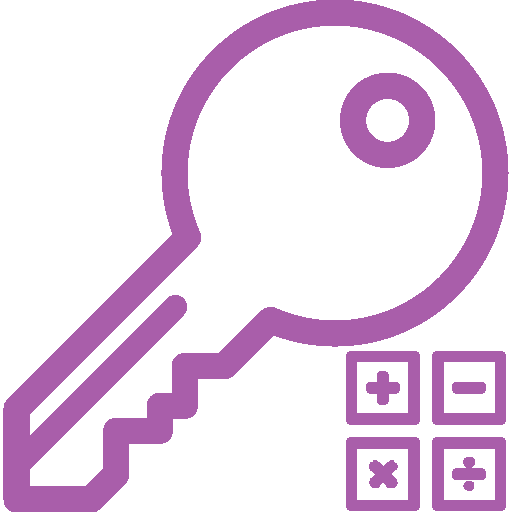
\includegraphics[width=\sizeindice cm]{img/blocks_from_slides/assets/evaluation_key_bis.png} % Smaller image
		}
	};
}


% define the nodes
\newcommand{\keygenfhe}[1]{\node[draw=\fhecolor, rectangle, very thick, minimum size = \sizenode cm] at (#1)(keygen) {$\textsf{KeyGen}_{\textsf{\gls{FHE}}}$};}

\newcommand{\encsym}[1]{\operatorwithimage{\symcolor}{enc_sym}{#1}{$\textsf{Enc}_{\textsf{Sym}}$}{red_key.png}}
\newcommand{\encfhe}[1]{\operatorwithimage{\fhecolor}{enc_fhe}{#1}{$\textsf{Enc}_{\textsf{\gls{FHE}}}$}{green_key.png}}
\newcommand{\decfhe}[1]{\operatorwithimage{\fhecolor}{dec_fhe}{#1}{$\textsf{Dec}_{\textsf{\gls{FHE}}}$}{green_key.png}}

\newcommand{\fheneuralnetwork}[1]{\homomorphicoperator{\fhecolor}{fhe_neural_network}{#1}{
	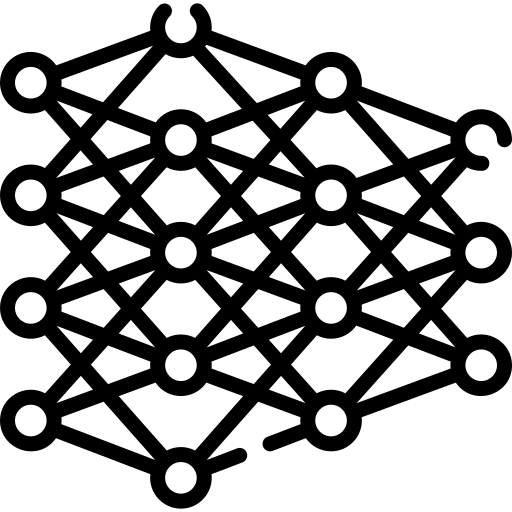
\includegraphics[width=\sizenode cm]{img/blocks_from_slides/assets/neural_network.png}
}}
\newcommand{\transciphering}[1]{\homomorphicoperator{\fhecolor}{transciphering}{#1}{$\textsf{Dec}_{\textsf{Sym}}^{(\textsf{\gls{FHE}})}$}}



\newcommand{\encrypteddata}[1]{\encryptedvalue{data.png}{\symcolor}{#1}{data_sym}}
\newcommand{\fhedata}[1]{\encryptedvalue{data.png}{\fhecolor}{#1}{data_fhe}}
\newcommand{\encryptedkey}[1]{\encryptedvalue{red_key.png}{\fhecolor}{#1}{encrypted_key}}
\newcommand{\fheresult}[1]{\encryptedvalue{results.png}{\fhecolor}{#1}{result_fhe}}
¨

\newcommand{\bootstrappingkey}[1]{\encryptedvalue{green_key.png}{\fhecolorbis}{#1}{bootstrapping_key}}
\newcommand{\bootstrapping}[1]{\homomorphicoperator{\fhecolorbis}{bootstrapping}{#1}{$\textsf{Dec}_{\textsf{\gls{FHE}}}$}}
\newcommand{\fhedatabis}[1]{\encryptedvalue{data.png}{\fhecolorbis}{#1}{data_fhe_bis}}
\newcommand{\polynomial}[4]{% #1 = x position, y_position, #3 = number of squares, label
	\foreach \j in {0,...,\numexpr#3-1\relax} {
		\draw (#1+\j, #2) rectangle (#1+\j+1, #2+1);
	}
	  \node[anchor=center, inner sep=2pt] (#4) at (#1 + #3/2, #2+0.5) {};
}

\newcommand{\coloredPolynomial}[4]{% #1 = x position, y_position, #3 = number of squares, label
	\foreach \j in {0,...,\numexpr#3-1\relax} {
		\draw[fill=blue, opacity=10] (#1+\j, #2) rectangle (#1+\j+1, #2+1);
	}
	\node[anchor=center, inner sep=2pt] (#4) at (#1 + #3/2, #2+0.5) {};
}


	\def\numSquares{5}
\def\spacingPoly{2}


\newcommand{\mvbFigureA}{
	\begin{tikzpicture}[scale=0.5, transform shape]
		\foreach \i in {0,...,3} {
			\pgfmathsetmacro{\xpos}{(\numSquares + \spacingPoly) * \i}
			\polynomial{\xpos}{0}{\numSquares}{poly\i}
			
			\coloredPolynomial{\xpos}{-2}{\numSquares}{polyBis\i}
			
			\draw[->, thick] (poly\i.south) -- (polyBis\i.north);
			
			\node[anchor=west] at (\xpos + \numSquares/2, -0.5) {\BlindRotate};
		}
	
	\end{tikzpicture}
}


\newcommand{\mvbFigureB}{
	\begin{tikzpicture}[scale=0.5, transform shape]
		\pgfmathsetmacro{\xpos}{(\numSquares + \spacingPoly) * 1.5}
		\polynomial{\xpos}{-4}{\numSquares}{polyBeforeMVB}
		
		\coloredPolynomial{\xpos}{-6}{\numSquares}{polyDuringMVB}
		\draw[->, thick] (polyBeforeMVB.south) -- (polyDuringMVB.north);
		\node[anchor=west] at (\xpos+ \numSquares/2 , -4.5) {\BlindRotate};
		
		\foreach \i in {0,...,3} {
			\pgfmathsetmacro{\xpos}{(\numSquares + \spacingPoly) * \i}
			\coloredPolynomial{\xpos}{-9}{\numSquares}{polyAfterMVB\i}
	
			\draw[->, color=purple, thick] ($(polyDuringMVB.south) + (0, -0.5)$) -- (polyAfterMVB\i.north);
			
			\node[anchor=west] at (\xpos + 1, -7.7) {\huge $\times v_\i$};
		}
	\end{tikzpicture}
}

% General box drawer
  % #1: coordinate
% #2: fill color
% #3: label
% #4: h-bracket label
% #5: v-bracket label
% #6: node name
% #7: width
% #8: height
\newcommand{\drawBoxAt}[8]{%
	\node[draw, anchor=north west, minimum width=#7cm, minimum height=#8cm, fill=#2] (#6) at #1 {#3};
	
	% Optional brackets
	\ifx&#4&%
	\else
	\draw[decorate,decoration={brace,mirror,amplitude=8pt}]
	(#6.south west) -- (#6.south east)
	node[midway,below,yshift=-10pt] {\( #4 \)};
	\fi
	
	\ifx&#5&%
	\else
	\draw[decorate,decoration={brace,amplitude=8pt}]
	(#6.south west) -- (#6.north west)
	node[midway,left,xshift=-10pt] {\( #5 \)};
	\fi
}

% Identity and base matrix shorthands
\newcommand{\identityMatrixAt}[2]{%
	\drawBoxAt{#1}{gray!30}{\texttt{Triv}}{n}{s^n}{#2}{1.5}{4}
}

\newcommand{\baseMatrixAt}[2]{%
	\drawBoxAt{#1}{green!30}{\texttt{Eval}}{\lambda}{}{#2}{4}{4}
}

\newcommand{\AMatrix}[2]{
	\drawBoxAt{#1}{purple!30}{\( \mat A^{(#2)} \)}{t_#2 \cdot n_#2}{s^n}{A#2}{7}{4}
}

\newcommand{\UMatrix}[2]{%
	\identityMatrixAt{#1}{U#2id}
	\baseMatrixAt{($ (U#2id.north east) + (0,0) $)}{U#2base}
	\draw[decorate,decoration={brace,amplitude=8pt}]
		(U#2id.north west) -- (U#2base.north east)
		node[midway,above,yshift=10pt] {\( n_#2 \)};
}


\newcommand{\UMatrixBis}[2]{%
	\pgfmathsetmacro{\plusOne}{int(#2 + 1)}
	\identityMatrixAt{#1}{U#2idBis}
	\baseMatrixAt{($ (U#2idBis.north east) + (0,0) $)}{U#2baseBis}
	\PMatrix{($ (U#2baseBis.north east) + (0, 0) $)}{P#2}
	\draw[decorate,decoration={brace,amplitude=8pt}]
	(U#2idBis.north west) -- (P#2.north east)
	node[midway,above,yshift=10pt] {\( n_\plusOne \)};
}

\newcommand{\DMatrix}[3]{
	\drawBoxAt{#1}{yellow!30}{\(\mat{D}^{(#2)}\)}{n_#2}{t_#2}{D#2}{#3}{1}
}

\newcommand{\yVector}[1]{
	\drawBoxAt{#1}{orange!30}{\(\vec{y}^{(0)}\)}{}{s^n}{y}{1}{4}
}

\newcommand{\betaVector}[1]{
	\drawBoxAt{#1}{orange!30}{\(\boldsymbol{\beta}^{(0)}\)}{}{t_0 \cdot n_0}{beta}{1}{5}
}

\newcommand{\PMatrix}[2]{
	\drawBoxAt{#1}{yellow!30}{\( \mat P^{(0)} \)}{t_0}{}{#2}{1}{4}
}


% Example usage: draw the full picture
\newcommand{\figureHLUT}{
	\begin{tikzpicture}[scale=0.7, transform shape]
	
	% U0 et D
	\UMatrix{(0, 0)}{0};
	\DMatrix{($ (U0id.south west) + (0, -2) $)}{0}{5.5}
 
	
	% Truc
	\node[draw, minimum width=1cm, minimum height=1cm]  (truc)
			at ($ (D0.north east) + (4, 2) $) {$\left (\mat U^{(0)} \cdot (\mat D^{(0)})^T \right ) \slyusar \mat U^{(0)}$};
	\draw[->] (U0base.east) -- (truc);
	\draw[->] (D0.east) -- (truc);
	\node[ minimum width=1cm, minimum height=1cm]  (3. step) at ($ (truc.north west) + (-0.5, 0) $) {3.};
	
	%A
	\AMatrix{($ (truc) + (4,3) $)}{0}
	\draw[->] (truc) -- (A0.west);
	
	%Chain
	\node[draw, minimum width=1cm, minimum height=1cm]  (chain)
				at ($ (U0base.north) + (0, 2) $) {\(\Phi_{n, \lambda}\)};
	\draw[->] (chain) -- (U0base.north);
	\node[ minimum width=1cm, minimum height=1cm]  (1. step) at ($ (chain.north west) + (-0.5, 0) $) {1.};

	% Random draw for D^T
	\node[draw, minimum width=1cm, minimum height=1cm]  (draw0)
	at ($ (D0.south) + (-2, - 2) $) {\$};
	\draw[->] (draw0) -- (D0);
	\node[ minimum width=1cm, minimum height=1cm]  (2. step) at ($ (draw0.west) + (-0.5, 0) $) {2.};	


	%y
	\yVector{($ (A0.south) + (0, -4) $)}
	
%	Gauss Elimination
	\node[draw, minimum width=2cm, minimum height=2cm]  (gaussElimination)
			at ($ (y.west) + (-4, 1) $) {\texttt{GaussElimination}}		;	
	\draw[->] (y.west) -- (gaussElimination);
	\draw[->] (A0) -- (gaussElimination);
	\node[ minimum width=1cm, minimum height=1cm]  (4. step) at ($ (gaussElimination.north west) + (-0.5, 0) $) {4.};
	
%	beta
	\betaVector{($ (gaussElimination.west) + (-2, 1) $)}
	\draw[->] (gaussElimination.west) -- (beta);
	
%	Compute Product
	\node[draw, minimum width=2cm, minimum height=2cm]  (computeProducts)
	at ($ (beta.west) + (-5, -2) $) {\texttt{ComputeProducts}}		;	
	\draw[->] (beta) -- (computeProducts);
	\draw[->](A0.south west) -- (computeProducts);
	\node[ minimum width=1cm, minimum height=1cm]  (5. step) at ($ (computeProducts.north west) + (-0.5, 0) $) {5.};
	
	
% Deuxième étage
	\UMatrixBis{($ (U0id.south west) + (0, -12) $)}{0}
	\draw[->] (computeProducts) -- (P0.north);
	\node at ($ (U0baseBis.east) + (1, 0) $) {$\cdot$};
	\DMatrix{($ (U0idBis.south west) + (0, -2) $)}{1}{6.5}
	\node[ minimum width=1cm, minimum height=1cm]  (5. step) at ($ (U0idBis.north west) + (-0.5, 0) $) {6.};
	
	
%	Second Draw
	\node[draw, minimum width=1cm, minimum height=1cm]  (draw1)
	at ($ (D1.south) + (-2, -2) $) {\$};
	\draw[->] (draw1) -- (D1);

%	truc 2
	\node[draw, minimum width=1cm, minimum height=1cm]  (truc2)
	at ($ (D1.north east) + (3, 2) $) {$(\mat U^{(1)} \cdot (\mat D^{(1)})^T) \slyusar \mat U^{(1)}$};
	\draw[->] (P0.east) -- (truc2);
	\draw[->] (D1.east) -- (truc2);	

	%A
\AMatrix{($ (truc2) + (4,3) $)}{1}
\draw[->] (truc2) -- (A1.west);
	
	\end{tikzpicture}
}



%!TeX_ROOT=../thesis.tex

\chapter*{How to read this thesis ?}
\addstarredchapter{How to read this thesis ?}

The thesis begins by a brief section written in French, that introduces the topic and provides a summary of the contributions of this thesis.

Chapter \ref{chap:fhe} is an introduction presenting Fully Homomorphic Encryption (FHE), including some historical background and a review of the state of the art. Then, Chapter \ref{chap:spec_tfhe} introduces the TFHE cryptosystem in detail, presenting all its internal components and their functioning. In particular, its bootstrapping operation, which lies at the heart of its homomorphic capabilities, is described in depth.

In Chapter \ref{chap:negacyclicity}, we address one of TFHE’s fundamental issues: the negacyclicity problem. This is one of the main hurdles when using TFHE in practice, as it limits the performance of homomorphic operations and greatly complicates the design of homomorphic programs. We provide a formal presentation of the problem as well as an overview of the existing solutions found in the literature. We then introduce a new approach using a plaintext space of odd order, which resolves the negacyclicity issue while also enabling new functionalities for TFHE. This construction forms the foundation on which the rest of this thesis builds.

Chapter \ref{chap:p_encodings} presents a method to accelerate the evaluation of arbitrary Boolean functions in TFHE. The core technique of TFHE’s original paper performs one bootstrapping per logic gate in the function’s circuit. The problem is that this approach does not scale well when working with more complex functions or more inputs. To overcome this, we developed a new type of encoding, called $p$-encodings, which embed bits into a larger space. This allows multiple bits to be compressed into the same ciphertext by summing them, enabling evaluation of the entire function through a single bootstrapping. We develop algorithms to find suitable $p$-encodings for a given function. If the circuit is still too large, we also present an algorithm to decompose it into sub-blocks that can be processed using our method. To test this construction, we apply it to several cryptographic primitives and demonstrate significant performance improvements compared to the state of the art.

This work resulted in the publication:

\begin{center}
\fullcite{TCHES:BonPoiRiv24}
\end{center}

Chapter \ref{chap:hyppogriph} aims to improve the homomorphic implementation of the AES standard from the previous chapter. To do so, we exploit both Boolean and arithmetic representations and develop a general framework for efficiently switching between the two. This requires generalizing the encoding method from the previous chapter beyond the Boolean case to the arithmetic case, and adapting advanced homomorphic operators from the literature to this encoding strategy. This leads to the fastest AES implementation in the literature.

This work resulted in the publication:

\begin{center}
\fullcite{hippogryph}
\end{center}

The main target use case of Chapter \ref{chap:hyppogriph} is transciphering, a cryptographic technique that solves the problem of ciphertext expansion. When data is encrypted homomorphically, it occupies much more memory space and thus consumes more bandwidth when sent to a server. Transciphering addresses this issue: instead, the client encrypts the data using a conventional symmetric cipher, and the server homomorphically decrypts the data to bring it into the homomorphic domain. Experimental results show that using a standard cipher like AES is not very efficient; instead, one would prefer a cipher specifically designed to be efficiently evaluable under homomorphic encryption. This is exactly what we construct in Chapter \ref{chap:transistor}: we present our contribution to the design of \texttt{Transistor}, a stream cipher that is highly efficient under TFHE. We provide its specification and explain the rationale behind its design choices, including the use of an odd modulus. Most of the chapter is dedicated to analyzing the strong performance of \texttt{Transistor} in the homomorphic domain.

This work was published in:

\begin{center}
\fullcite{transistor}
\end{center}

The published version above includes significantly more content, including an in-depth security analysis of the scheme.

One of TFHE’s main limitations is that programmable bootstrapping becomes very slow as the size of the message increases. As a result, evaluating Look-Up Tables (LUTs) larger than 8 bits is impractical. In Chapter \ref{chap:larger_lut}, we tackle this issue by extending TFHE’s bootstrapping capabilities beyond 8 bits through a method that accelerates homomorphic evaluation of large LUTs. Once again leveraging our encoding technique, we design a LUT decomposition algorithm that enables bootstrapping to be applied on smaller messages.
\TODO{Details will be added once the chapter is written}

Finally, Chapter \ref{chap:parameters} goes beyond the scope of our encoding method in odd spaces and introduces \toolName, a tool designed to help homomorphic program designers choose parameter sets that ensure the three central properties: security, correctness of computation, and efficiency. The strength of \toolName lies in its flexibility, allowing easy extension to new homomorphic operators. Furthermore, its optimization algorithm estimates runtime using a cost model that depends on the machine executing the program, allowing parameter sets to be tailored to various usage contexts.
\TODO{Details will be added once written}

\cleardoublepage
%!TeX_ROOT=../thesis.tex

\chapter*{Introduction en Français}
\addstarredchapter{Introduction en Français}


\section{Mise en Contexte}

\paragraph{Cryptographie.} La \textit{cryptographie} est un domaine technique a l'interface entre l'informatique et les mathématiques appliquées. Elle étudie les méthodes permettant de protéger l'information. Les techniques cryptographiques les plus classiques sont:
\begin{itemize}
	\item Le \textit{chiffrement}, qui transforme un message, un fichier ou plus généralement n'importe quel type de donnée en la ``brouillant''. Le seul moyen pour déchiffrer est de posséder la \textit{clé} du chiffrement. La donnée est donc illisible par les personnes non autorisées, . Cette technique est notamment utilisée pour protéger la confidentialité des messages sur les applications de messageries instantanées telles que WhatsApp ou Signal.
	\item L'\textit{authentification}, qui permet de vérifier l'identité de l'émetteur d'un message. Par exemple, elle assure qu’un utilisateur se connecte bien au serveur de sa banque et non à un serveur frauduleux contrôlé par un pirate.
	\item Le \textit{contrôle d'intégrité}, qui permet de s'assurer qu'un message n'a pas été modifié ou corrompu pendant sa transmission. C'est notamment utile pour s'assurer qu'un logiciel téléchargé n'a pas été altéré afin d'y introduire une faille de sécurité.
\end{itemize}


A l'origine exclusivement réservée au domaine militaire, la cryptographie a été transformée en un enjeu de société majeur au XXIe siècle. Une grande partie des échanges se fait désormais en ligne, qu'il s'agisse de transactions bancaires, d'échanges commerciaux ou de simples messages à ses proches. De fait, rendre les systèmes de communications résistants face aux attaques d'acteurs malveillants est devenu  un enjeu stratégique central pour garantir la sécurité et les libertés individuelles des citoyens. Des exemples de tels attaquants sont les cybercriminels qui pratiquent l'usurpation d'identité pour monter des escroqueries, ou bien rançonnent des entreprises ou des services publics en bloquant leur infrastructure ou en retenant leurs données. Il s'agit aussi de gouvernements autoritaires pratiquant la surveillance de masse sur leur population, afin de neutraliser des opposants politiques ou opprimer des groupes minoritaires.

Les travaux fondateurs de Claude Shannon sur la théorie de l'information montrent qu'\textit{il ne peut exister de chiffrement parfait}. Autrement dit, un système cryptographique \textit{théoriquement incassable} serait inutilisable dans le monde réel. Ainsi, la pratique de la cryptographie consiste à garantir un niveau de sécurité suffisant à un système, sans altérer sa fonctionnalité ni ses performances.

Pour ce faire, les cryptographes cherchent à déterminer la puissance de calcul nécessaire à un attaquant pour casser un système de sécurité, par exemple en déchiffrant un message secret dont il n'a pas la clé. L'exemple le plus basique d'attaque est l'attaque par force brute (\textit{brute force}), qui consiste à essayer toutes les clés possibles jusqu'à trouver la bonne. Il convient donc de choisir des clés suffisamment grandes pour que cette stratégie soit trop lente, ou trop coûteuse à mettre en oeuvre. Evidemment, les attaques contre les systèmes cryptographiques se sophistiquent d'années en années, donc les techniques cryptographiques doivent évoluer pour s'y adapter et toujours avoir un temps d'avance.



\paragraph{Calculer sur des données chiffrées.}
La cryptographie a connu un essor fulgurant au cours des dernières décennies. Notamment, le trafic Internet, qui était en clair jusqu'alors, a été sécurisé par l'introduction du protocole HTTPS, qui permet de chiffrer et d'authentifier les échanges entre le client et le serveur.

Cependant, il reste un cas d'usage où la cryptographie demeure impuissante, et dans lequel les données sont encore mal protégées: le \textit{calcul délégué}. Cette (vague) dénomination englobe tout les cas d'usages dans lesquels un utilisateur envoie une donnée à un serveur, non pas pour qu'il en assure le transit à travers Internet, mais pour qu'il la traite et lui renvoie un résultat. On peut penser par exemple aux applications telle que Google Maps, dans lesquelles l'utilisateur envoie sa position actuelle et sa destination au serveur, qui calcule alors un itinéraire qu'il renvoie sur le téléphone de  l'utilisateur. On peut également penser aux nouvelles applications d'Intelligences Artificielles génératives dans lesquelles l'entrée de l'utilisateur est traitée par un algorithme pour générer du texte, de la musique ou des images. Enfin, cela concerne tous les cas où des entreprises louent des serveurs externes pour effectuer des calculs lourds ou héberger des services.
 Sebastian Vettel[S] [score hidden] an hour ago 
Le problème est qu'effectuer des calculs sur des données chiffrées est un immense défi technologique, qu'on a longtemps pensé impossible. Par conséquent, le serveur doit nécessairement déchiffrer les données pour pouvoir les traiter, ce qui rend ces dernières vulnérable à la moindre compromission du serveur par une attaque informatique.


\paragraph{Cryptographie Homomorphe.}
La cryptographie homomorphe (\textit{Fully Homomorphic Encryption} en anglais, souvent abrégé en FHE) est la branche de la cryptographie qui s'attaque à ce problème. Son but est de développer des algorithmes de chiffrement permettant à un serveur d'effectuer des calculs directement sur les données chiffrées, sans nécessiter de déchiffrement préalable. Il devient alors inutile pour un attaquant d'essayer de s'y introduire, car l'intégralité des données de valeur qu'il contient sont chiffrées et donc inutilisables.De plus, le fournisseur du service n'a lui-même pas accès aux données, ce qui assure une confidentialité totale vis-à-vis de l'utilisateur.

Cette idée apparaît dans un article de recherche pour la première fois en 1978, mais il faut attendre 2009 pour que la première construction viable d'un algorithme de chiffrement homomorphe apparaisse dans un article de recherche intitulé \textit{Fully Homomorphic Encryption from Ideal Lattices} par Craig Gentry \cite{STOC:Gentry09}. Ce travail a surtout une valeur théorique, car l'algorithme de Gentry demande tellement de ressources pour être calculé qu'il est impossible de l'utiliser dans le monde réel.

Cet article a initié un veritable essor du domaine dans la communauté scientifique, et les progrès ont été extrèmement rapides. Les algorithmes actuels commencent à être utilisable en pratique, et certains projets concrets d'aapplications homomorphes commencent à voir le jour.

Le challenge actuel est donc d'améliorer les performances du chiffrement homomorphe. Pour cela, les cryptographes doivent s'attaquer à deux problématiques principales:

\begin{itemize}
	\item \textit{La quantité de calcul nécessaire:} Effectuer un calcul dans le domaine homomorphe (c'est-à-dire directement sur les chiffrés) nécessite beaucoup plus d'opérations que lorsqu'on l'effectue en clair. Par conséquent, une application fonctionnant homomorphiquement est beaucoup plus lente et plus coûteuse en énergie que si on l'exécute de façon classique (de 3 à 5 ordres de grandeur en fonction de la nature des calculs). 
	\item \textit{Le bruit:} La sécurité des schémas de chiffrement homomorphes reposent sur la théorie des réseaux euclidiens. Concrètement, cela signifie que lorsqu'on chiffre les données on leur ajoute une petite perturbation aléatoire qu'on appelle le \textit{bruit}. Comme ce bruit est très faible, il ne pose pas de problème lors du déchiffrement car il est facile de se débarasser de cette imprécision en arrondissant simplement les valeurs. Par contre, lorsqu'on effectue des calculs homomorphes entre plusieurs valeurs chiffrées, leurs bruits s'additionnent ce qui fait croître l'imprécision. Par conséquent, le nombre d'opérations homomorphes qu'il est possible d'effectuer est limité, car un bruit trop élevé deviendrait prépondérant par rapport à l'information contenue dans les messages, rendant le déchiffrement impossible. On a donc un ``quota'' de quantité de calculs disponible  au terme duquel il faut nécessairement s'arrêter.
\end{itemize}


\paragraph{Bootstrapping.}
Dans son article fondateur de 2009, Craig Gentry introduit une notion fondatrice appelée \textit{bootstrapping}\footnote{on dirait \textit{réamorçage} en français}, qui résout complètement le second problème. Il s'agit d'une opération qui permet au serveur de réduire le bruit d'un chiffré de manière homomorphe, sans violer la confidentialité des données ! Donc si un schéma de chiffrement possède une opération de bootstrapping (on dit qu'il est \textit{bootstrappable}), cela signifie qu'il n'a pas de limitations sur la quantité de calcul qu'il est possible de faire sur les données chiffrées. En effet, il suffit d'appliquer un bootstrapping à chaque fois que la quantité de bruit dans les chiffrés devient trop grande, et de continuer les calculs avec le chiffré bootstrappé !


Pour comprendre comment cela fonctionne, rappelez vous que lorsque l'utilisateur déchiffre le résultat, il élimine le bruit avec une opération d'arrondi. Donc, si il est possible de calculer homomorphiquement la fonction de déchiffrement du schéma, alors il est possible de retirer le bruit sans que le serveur aie besoin de déchiffrer ! 

Concrètement, disons que le serveur possède un message chiffré $\vec c_1$ qui correspond au message clair (bruité) $m + e_1$, chiffré avec la clé secrète $\vec s_1$. Ici $m$ et $e_1$ représentent respectivement le message clair et le bruit. Supposons que $\vec c_1$ soit le résultat d’opérations homomorphes, donc le bruit $e_1$ est élevé. Si nous voulons continuer à calculer, il faut réduire le bruit par un processus de bootstrapping.
Pour cela, le client doit fournir au serveur une clé de bootstrapping $\BSK$. Pour la créer, le client peut considérer la clé secrète $\vec s_1$ comme un message et la chiffrer sous une autre clé secrète $\vec s_2$ pour produire $\BSK = \texttt{Enc}_{\vec s_2}(\vec s_1)$, où \texttt{Enc} désigne la fonction de chiffrement.

La propriété fondamentale découverte par Gentry est que si le serveur calcule homomorphiquement le déchiffrement de $\vec c_1$ en utilisant la clé $\BSK$, il obtient un chiffré $\vec c_2$ du même message sous la clé secrète $\vec s_2$. Mais comme le déchiffrement élimine le bruit, $e_1$ disparaît et le message chiffré est à nouveau « frais » !
En réalité, tout le bruit n’est pas supprimé (ce qui ne serait pas souhaitable, car toute la sécurité du chiffrement repose sur la présence de bruit dans les chiffrés). Comme il y a du bruit dans $\BSK$, le résultat $\vec c_2$ contient un nouveau bruit $e_2$. Mais si l'algorithme est bien conçu, il est possible d’avoir $e_2 \ll e_1$, ce qui permet de gagner de la marge pour d’autres calculs.


Le bootstrapping n'est cependant pas une solution miracle. En effet, c'est une opération extrèmement coûteuse pour la totalité des schémas de chiffrement homomorphe. Donc en résolvant le second problème (celui du bruit qui limite la quantité de calcul), nous avons en fait aggravé le premier (la lenteur du FHE) ! L'un des axes de recherches principaux dans la communauté scientifique est donc de créer des schémas de chiffrement homomorphe avec un bootstrapping le plus efficace possible. 



\paragraph{Le schéma TFHE}
L'un des schémas homomorphes les plus prometteurs se nomme TFHE \cite{JC:CGGI20} (pour \textit{Fully Homomorphic Encryption over the Torus}). Comme tous les autres schémas, il permet d'effectuer des opérations linéaires, c'est-à-dire l'addition de deux chiffrés et la multiplication d'un chiffré par une constante. Ces opérations linéaires sont quasiment gratuites en terme de quantité de calcul, donc sont extrèmement rapides. Par contre, elles augmentent le bruit dans les chiffrés, et le serveur ne peut donc pas en effectuer un nombre illimité. Fort heureusement, TFHE possède une opération de bootstrapping relativement efficace par rapport aux standards du FHE, et donc les chiffrés peuvent être régulièrement rafraîchi sans tuer les performances. 
La particularité du bootstrapping de TFHE est qu'il est \textit{programmable}. Cela signifie qu'en plus de réduire le niveau de bruit, le bootstrapping permet d'évaluer n'importe quelle fonction sur le chiffré, sans aucun surcoût ni en terme de calculs ni en terme de bruit ! Cette fonctionnalité représente une avancée majeure dans le domaine, car cela permet de rentabiliser le temps passé dans les opérations de bootstrapping.

Cependant, TFHE a deux défauts de taille par rapport aux autres schémas de l'état de l'art. D'abord, il ne permet de manipuler des données de faible précision, de l'ordre de quelques bits. Par conséquent, si on veut travailler avec des entiers, cela nécessite de découper les valeurs en petites ``tranches'' de quelques bits et de manipuler ces sous-blocs. Cela rend la conception de programmes homomorphes bien plus complexe que dans le domaine des clairs. C'est la raison pour laquelle le développement de systèmes de compilation automatique de programmes homomorphes est devenu un domaine de recherche actif ces dernières années.

Le second problème est que TFHE n'est pas intrinsèquement parallélisable, contrairement à d'autres chiffrements prometteurs de l'état de l'art tels que CKKS \cite{AC:CKKS17} qui permettent d'encoder plusieurs valeurs dans un même chiffré et d'effectuer des calculs en parallèle sur chacun d'eux. Si ces schémas montrent des meilleurs timings amortis, leur latence est beaucoup plus grande.


Malgré ces faiblesses, TFHE reste très étudié dans la littérature scientifique et constitue l'un des principaux espoirs pour l'adoption massive du chiffrement homomorphe. Pendant cette thèse, nous nous sommes concentrés sur ce schéma et avons développé des algorithmes permettant d'accélérer les calculs homomorphes dans certains cas d'usages. Nous présentons un résumé de nos travaux dans la prochaine section.




\section{Résumé de la thèse et des contributions scientifiques}

La thèse commence par une introduction (Chapitre \ref{chap:fhe}) présentant le chiffrement totalement homomorphe, incluant quelques considérations historiques et présentant un état de l’art. Puis, le chapitre \ref{chap:spec_tfhe} introduit en détail le cryptosystème TFHE, en présentant tous ses composants internes ainsi que leur fonctionnement. En particulier, son opération de bootstrapping, qui constitue le coeur de ses capacités homomorphes, est présenté en détail.


Dans le chapitre \ref{chap:negacyclicity}, nous présentons l'une des problématiques fondamentales de TFHE: \textit{le problème de négacyclicité}. Il s'agit de l’un des principaux éceuils lors de l'utilisation de TFHE en pratique,  car il limite les performances des opérations homomorphes de TFHE et complexifie énormément la conception de programmes homomorphes. Nous donnons une présentation formelle du problème ainsi qu’un aperçu de l’état de l’art des solutions existantes dans la littérature pour le résoudre. Puis, nous introduisons une nouvelle méthode consistant à utiliser un espace de plaintext d'ordre \textit{impair}, ce qui résout ce problème de négacyclicité tout en activant de nouvelles fonctionnalités pour TFHE. Cette construction constitue la base sur laquelle reposent les contributions du reste de cette thèse.


Le chapitre \ref{chap:p_encodings} présente une méthode pour accélérer l’évaluation de fonctions booléennes arbitraires en TFHE. La technique de base de l'article fondateur de TFHE est d'effectuer un bootstrapping par porte logique dans le circuit de la fonction. Le problème est que cette stratégie passe très mal à l'échelle quand on veut travailler avec des fonctions plus complexes ou avec plus d'entrées. Pour résoudre ce problème, nous avons développé un nouveau type d'encodage, appelé \textit{$p$-encodages}, qui plongent les bits dans un espace plus grand. Grâce à cela, il devient possible de compresser plusieurs bits dans le même chiffré en les sommant, puis d'évaluer l'intégralité de la fonction en ne calculant qu'un seul bootstrapping. Nous développons des algorithmes permettant de trouver les $p$-encodages adaptés à une fonction donnée. Dans le cas où le circuit serait tout de même trop grand, nous présentons également un algorithme pour découper le circuit en sous-blocs évaluables avec notre méthode. Pour tester notre construction, nous l'appliquons à quelques primitives cryptographiques pour les implémenter en homomorphe, et démontrons un gain de performance significatif par rapport à l’état de l’art.
Ce travail a donné lieu à la publication:

\begin{center}
	\fullcite{TCHES:BonPoiRiv24}
\end{center}

Le chapitre \ref{chap:hyppogriph} vie à améliorer l'implémentation homomorphe du standard AES du chapitre précédent. Pour ce faire, nous exploitons à la fois les représentations booléennes et arithmétiques et développons un cadre générique pour passer efficacement de l’une à l’autre. Cela nécessite de généraliser la méthode d’encodage du chapitre précédent au-delà du cas booléen vers le cas arithmétique, ainsi que d'adapter des opérateurs homomorphes avancés de l'état de l'art à cette logique d'encodage. Nous produisons ainsi l'implémentation d’AES la plus rapide de la littérature.
Ce travail a donné lieu à la publication:

\begin{center}
	\fullcite{hippogryph}
\end{center}

Le principal cas d'usage visé par le chapitre \ref{chap:hyppogriph} est le transchiffrement, une technique cryptographique permettant de résoudre le problème d'expansion de chiffré. Concrètement, lorsque des données sont chiffrées homomorphiquement, elles prennent beaucoup plus d'espace en mémoire, et donc consomment plus de bande passante quand elles sont envoyées au serveur. Le transchiffrement résout ce problème: le client va plutôt envoyer les données chiffrées avec un algorithme de chiffrement symétrique classique, et le serveur va déchiffrer homomorphiquement ces données pour les récupérer dans le domaine homomorphe. LEs résultats expérimentaux montrent qu'utiliser un chiffrement standard tel que l'AES n'est pas très performant, au lieu de cela on préfèrerait utiliser un algorithme de chiffrement spécialement conçu pour s'évaluer rapidement dans le domain homomorphe. C'est ce que nous construisons dans le chapitre \ref{chap:transistor}: nous y présentons notre constribution à la conception de \texttt{Transistor}, un chiffrement à flot s'évaluant très efficacement avec TFHE.  Nous en donnons la spécification et expliquons le raisonnement motivant ses choix de conception, notamment l'utilisation du modulo impair. La majeure partie de ce chapitre est consacrée à l’analyse des bonnes performances de \texttt{Transistor} dans le domaine homomorphe.
Ce travail a donné lieu à une publication dans

\begin{center}
	\fullcite{transistor}
\end{center}

La version publiée ci-dessus a beaucoup plus de contenu, notamment une analyse approfondie de la sécurité du schéma.


L'une des limitations principales de TFHE est que l'opération de bootstrapping programmable devient très lente à mesure qu'on traite des messages de plus en plus grands. Ainsi, évaluer des tables de correspondances (\textit{Look-Up Tables}) de taille supérieure à 8 bits est impossible en pratique.  Dans le chapitre \ref{chap:larger_lut}, nous nous attaquons à ce problème et étendons les capacités du bootstrapping de TFHE au-delà de 8 bits grâce à une méthode accélérant l’évaluation homomorphe de ces grandes \textit{Look-Up Tables}. En nous appuyant à nouveau sur notre technique d'encodage, nous avons conçu un algorithme de décomposition des LUT permettant d'utiliser le bootstrapping sur des plus petits messages. 
\TODO{Détailler quand le chapitre sera écrit}



Enfin, le chapitre \ref{chap:parameters} va au-delà du cadre de notre méthode d'encodage dans des espaces impairs et introduit \toolName, un outil destiné à aider les concepteurs de programmes homomorphes à dimensionner des jeux de paramètres garantissant les trois propriétés centrales : la sécurité, la correction des calculs et l’efficacité. La force de \toolName réside dans sa flexibilité permettant de l'étendre facilement à des nouveaux opérateurs homomorphes. De plus, son algorithme d'optimisation estime le temps de calcul grâce à un modèle de coût dépendant de la machine sur laquelle le programme tourne, permettant d'adapter les jeux de paramètres à différents contextes d'utilisation.
\TODO{Détailler quand ce sera écrit}




\chapter{Introduction: Fully Homomorphic Encryption}



\section{Why ?}





\section{Historical Background}



\TODO{a section on security properties (ind-cpa-d, cca, etc...)}



\section{The bootstrapping : breakthrough construction}




%!TeX_ROOT=../thesis.tex

\chapter{Presentation of the TFHE Scheme}
\label{chap:spec_tfhe}

The previous chapter presented insights on Fully Homomorphic Encryption in general, but this thesis will exclusively cover the TFHE scheme.

Presented in \cite{JC:CGGI20, these_chillotti} as an evolution of the FHEW scheme \cite{EC:DucMic15}, TFHE quickly gained traction to become one of the most promising scheme to attain performances good enough to be  used in real-world scenarios. 

At the core of TFHE lies a powerful \textit{Programmable Bootstrapping} operation (PBS). As we presented in Section \ref{sec:gentry_bootstrapping}, it allows to manage the noise in the ciphertexts during the computation, allowing to achieve Fully Homomorphic Encryption. In TFHE, this bootstrapping operation goes a step further: it enables the evaluation of arbitrary functions directly on the refreshed ciphertexts, with no computational or noise overhead.

In this chapter we provide an in-depth presentation of the TFHE scheme. We introduce the hardness assumptions it relies on, its encryption procedure as well as its homomorphic capabilities. We conclude with insights into its practical performance.

\section{Hardness Assumptions: $\LWE$ and $\GLWE$ Problems}
\label{sec:hardness_assumptions}


\paragraph{Original $\LWE$ problem.}

In 2005, Regev laid the foundations for an important part of modern lattice-based cryptography by defining the Learning With Errors ($\LWE$) problem in \cite{regev_lwe}. The version usually used in FHE literature is presented in Definition \ref{def:LWE}:


\begin{definition}
	(Learning with Errors). Let $q$ and $n$ two integers, respectively called \textit{modulus} and \textit{dimension}.  Let $\chi_s$ and $\chi_e$ be distributions over \textit{small} values of $\lweRing$. We consider a secret vector, sampled as: $\lweSecretKey = (s_0, \dots, s_{n-1}) \drawfrom \chi_s^n$. The $\LWE$ distribution $\mathcal{D}_{q, n, \chi_s, \chi_e}^{\LWE}(\lweSecretKey)$ is defined as:
	
	 \[
	 \mathcal{D}_{q, n, \chi_s, \chi_e}^{\LWE}(\lweSecretKey) = \left \{(\vec a, b) \;\middle|\; \vec a = (a_0, \dots, a_{n-1}) \drawfrom \unif{\lweRing}^n, e \drawfrom \chi_e, b = \innerProduct{\vec a}{\vec s} + e \right \}
	  \]
	 
	 The \textit{decisional} version of the problem is to distinguish this distribution from a uniformly random one, namely:
	
	\[
	\mathcal{D}^{(\textsf{random})} = \left \{(\vec a, r) \;\middle|\; \vec a \drawfrom \unif{\lweRing}^n, r \drawfrom \unif{\lweRing} \right\}
	\]

	The \emph{search} version of the problem is to recover $\lweSecretKey$ from samples of $\mathcal{D}_{q, n, \chi_s, \chi_e}^{\LWE}(\lweSecretKey)$. 
	\label{def:LWE}
\end{definition}


Regev proved that the search and decisional problems are reducible to each other and their average case is as hard as worst-case lattice problems.

The hardness of this problem depends on the parameters $q$, $n$, $\chi_s$ and $\chi_e$, and so does the security of the schemes built upon it. There is not yet in the literature simple guidelines to construct secure instances of the problem. Common practice in the field is to derive an approximate concrete security level $\lambda$ for a given parameter set with a tool named \texttt{lattice-estimator} \cite{lattice-estimator}. Users can input concrete values and distributions for the parameters, and the tool evaluates the security of the underlying $\LWE$ instance by running simulations of attacks of the literature.

In Definition \ref{def:LWE}, we did not specify the shapes of the distributions $\chi_s$ and $\chi_e$ (beyond the fact they yields small values). Several distributions are possible: a discrete Gaussian with a small variance, a uniform distribution restricted on a small interval, or a binomial. Some versions with sparse secrets also exist. The choice of the right distribution depends of the considered use-case, each possibilities offering different trade-offs in matter of security and efficiency \cite{AFRICACRYPT:BGPW16, DBLP:conf/ccs/CurtisP19, EPRINT:BGPT19, EPRINT:SLZS24}.


Most implementations of TFHE select a uniform distribution on $\{0, 1\}$ for the secret, and a Gaussian with a small variance $\lweSigma^2$ for the noise. We will use these distributions in this thesis, and will use the notation $\LWE_{(q, n, \sigma)}$ for these instances.



\paragraph{Extension to the Polynomials.}


Looking for more efficient solutions, $\LWE$ problem has been declined in a \textit{ring variant} named $\RLWE$ in \cite{rlwe}. A generalized version over rings named $\GLWE$, first formalized in \cite{EPRINT:BraGenVai11} and used by TFHE, is presented below. It is very similar to the $\LWE$ one, but deals with polynomial values instead of integers:

\begin{definition}
	(Generalized Learning with Errors) Let $q$, $k$ and $N$ three integers, respectively called \textit{modulus}, \textit{dimension} and \textit{degree}. We consider the polynomial ring $\glweRingFull$, that we denote in short $\glweRing$. Let $\chi_S$ and $\chi_E$ be distributions over the small values of $\glweRing$, (that is to say, polynomials with small coefficients). We consider a secret vector $\glweSecretKey$, sampled as $\glweSecretKey = (S_0, \dots, S_{k-1}) \drawfrom \chi_S^k$. The $\GLWE$ distribution $\mathcal{D}_{q, k, N, \chi_S, \chi_E}^{\GLWE}(\glweSecretKey)$ is defined as:
	
	\[
	\mathcal{D}_{q, k, N, \chi_S, \chi_E}^{\GLWE}(\glweSecretKey) = \left \{ (\vec A, B) \;\middle|\; \vec A = (A_0, \dots, A_{k-1}) \drawfrom \unif{\glweRing}^k, E \drawfrom \chi_E, B = \innerProduct{\vec A}{\vec S} + E \right \}
	\]
	
	The \textit{decisional} version of the problem is to distinguish this distribution from a uniformly random one, namely:
	
	\[
	\mathcal{D}^{(\textsf{random})} = \left \{(\vec A, R) \;\middle|\; \vec A \drawfrom \unif{\glweRing}^k, R \drawfrom \unif{\glweRing} \right\}
	\]
	
	The \emph{search} version of the problem is to recover $\lweSecretKey$ from samples of $\mathcal{D}_{q, k , N, \chi_S, \chi_E}^{\GLWE}(\glweSecretKey)$. 
	\label{def:GLWE}
\end{definition}

Note that if we fix $k = 1$, we fall back on the classical $\RLWE$ problem, notably used in BGV \cite{bgv}. Also, taking $N=1$ produces a $\LWE$ instance with $n = k$. 

Concretely, using polynomial rings allows to encode more information in a single sample, yielding more compact ciphertexts and public keys. The schemes can also benefit from high-speed polynomial arithmetic techniques such as Fast Fourier Transforms (FFT). 

General consensus is that hardness of an instance $\GLWE_{(q, k, N, \sigma)}$ is similar to the hardness of $\LWE_{(q, k \cdot N, \sigma)}$, which makes possible to use the \texttt{lattice-estimator} as well.


\section{Torus Equivalence and Discretization}
\label{sec:torus_equivalence}


The T in TFHE stands for \textit{Torus}, because in the seminal paper of TFHE \cite{JC:CGGI20}, authors worked with torus-based variants of $\LWE$ and $\GLWE$.


The torus $\T = \R / \Z$ corresponds to the reals modulo 1. Algebraically, this space does not have a ring structure, but actually is a \textit{$\Z$-module} one, which means that:

\begin{itemize}
	\item The sum of two torus elements is well-defined, and yields another torus element.
	\item The multiplication between an element of $\T$ and an element of $\Z$ is also well-defined, and produces an element of $\T$.
	\item On the other hand, multiplying two elements of $\mathbb T$ does not make sense. To be convinced of it, we can remark that, for any non-zero torus element $x$, $0 \times x = 0$ while $1 \times x = x$. But since 0 and 1 are equivalent over the torus, these results should not be different. 
\end{itemize}



Recall the $\LWE$ assumption (Definition \ref{def:LWE}). If we rescale the elements of $\lweRing$ by dividing them by $q$, we get torus elements. We can then redefine seamlessly the $\LWE$ problem over the torus. Extensive details about this transformation can be found in \cite{these_chillotti}.


This brings two advantages:

\begin{itemize}
	\item $\LWE$ over the torus is \textit{scale-invariant}, which makes the analysis of the security and of the noise much simpler.
	\item The $\Z$-module structure propagates in the ring versions, as well as in matrices spaces. Thus, it allows for very powerful generalizations of homomorphic schemes on a wide variety of spaces, like in \cite{chimera, chimera2}.
\end{itemize} 


When implementing the scheme in practice, torus elements are represented by integers in machine. The torus is thus seen as \textit{discretized}, which we denote by 

\[ \T_q = \left \{   \frac a q \;\middle|\; a \in \Z_q  \right \} \] 

with $q = 2^\Omega$ ($\Omega$ denotes the number of bits of precision of the type, so 32 or 64 bits in most implementations). The properties of the torus structure are preserved.


This thesis is mainly about practical instantiations of the scheme. So, for the sake of clarity we will adopt a notation closer to the reality of the objects manipulated in machine. So the torus elements will be seen as elements of $\lweRing$ (but keeping the algebraic rules imposed by the structure of $\T$), and the same will be applied for ring extensions. 



\section{Encryption and Decryption in TFHE}
\label{sec:encryption}

\paragraph{Spaces.}

To understand the encryption procedure of TFHE, we must first introduce its plaintext space and its ciphertext space, and how the former can be embedded into the latter.

The plaintext space of TFHE is the \textit{discretized torus} $\plaintextTorus$. As explained in Section \ref{sec:torus_equivalence}, we trivially identify it to the ring $\plaintextRing$ with $p$ an integer. Conversely, the ciphertext space is the discretized torus $\lweTorus$ introduced in the previous section identified to a ring $\lweRing$, with $q = 2^\Omega$. In practice, $p \ll q$.


We need a way to encode plaintext values into the ciphertext space. To do so, let us consider a mapping $\rho: \plaintextRing \rightarrow \lweRing$, defined as \[
\rho: m  \mapsto \rounding{\frac{m \cdot q} {p}}.
\]


The image of this mapping only reaches $p$ elements in $\lweRing$, forming the set $\left \{ \rounding{\frac {k q}{p}} \mid k \in \plaintextRing \right \}$. These elements are distributed around $\lweRing$ and form what we refer to as \emph{sectors of $\lweRing$}, defined as: \[
\left\{ \left( \frac{(2k - 1)q}{2p}, \frac{(2k + 1)q}{2p} \right) ~\middle|~ k \in \mathbb{Z} \right\}
\]. A representation of such a mapping is shown on Figure \ref{fig:example_encoding}.

To encode a given plaintext element $m$ into the ciphertext space, we use the corresponding center of sector $\rounding{\frac{mq}{p}}$. However, decoding is more permissive: every elements of a sector are decoded by the corresponding plaintext element. This will be useful to remove the noise in ciphertexts.

\begin{figure}[htbp]
	\centering
	\wrappedTorus{64}{8}{true}
	\caption{An example of embedding of $\Z_8$ into $\Z_{64}$}
	\label{fig:example_encoding}
\end{figure}

We can now move to the actual encryption and decryption algorithms. TFHE features two main types of encryption: $\LWE$ encryption and $\GLWE$ encryption. Both share similar structural patterns but operate within different mathematical spaces.

\paragraph{LWE Encryption.}
$\LWE$ encryption deals with scalar values. The plaintext space is $\plaintextRing$ and the secret key is sampled uniformly at random from $\B^n$. We denote by $q$ the ciphertext modulus. We also need 
$\chi_{\lweSigma}$, a centered Gaussian distribution of standard deviation $\lweSigma$ in $\lweRing$. The encryption algorithm produces a ciphertext $\vec c$ of the form:

\begin{definition}($\LWE$ ciphertext)
	A $\LWE$ ciphertext encrypting a message $m \in \plaintextRing$ under a secret key $\lweSecretKey=(s_0, \dots, s_{n-1}) \in \B^n$ has the form:
	
	\begin{equation}
		\vec c = \LWE_{\lweSecretKey}(m) = \left (a_0, \dots, a_{n-1}, b = \sum_{i=0}^{n-1} a_i \cdot s_i + \tilde m + e \right ) \in \lweRing^{n+1}
	\end{equation}
	where:
	\begin{itemize}
		\item the elements $\vec a = (a_0, \dots, a_{n-1})$ are sampled uniformly at random in $\lweRing$.

		\item $\tilde m$ is the message encoded in the ciphertext space: $\tilde m = \rho(m) \in \lweRing$.
		\item $e$ is a small random Gaussian noise sampled from $\chi_{\lweSigma}$.
	\end{itemize}
\end{definition}


Decryption is performed in two steps: first, we compute the \emph{phase} of the ciphertext as $\phi(\vec c) = b - \langle \vec a, \vec s\rangle$. The phase corresponds to the noisy message $\tilde{m} + e$. To recover the actual message, we simply decode the phase by looking up the plaintext element corresponding to the sector. This can be interpreted as a rounding: $m = \rounding{\frac p q \phi(c)}$. 

As long as $|e| < \frac{q}{2p}$, this rounding produces the right sector center, and thus we recover the correct plaintext value. Otherwise the phase lies in a different sector and we recover a wrong value. It is thus very important to keep the noise level low enough to ensure correct decryption.


Security-wise, this encryption relies on the hardness of the assumption $\LWE_{(q, n, \lweSigma)}$. The dimensioning of these parameters should be handled properly to ensure security, correctness and efficiency. Chapter \ref{chap:parameters} of this thesis will be dedicated to this question.



\paragraph{GLWE Encryption.} This encryption mode mirrors the structure of $\LWE$ encryption but operates within polynomial rings.
This time, the plaintext space is $\plaintextTorusPoly$, identified with the ring $\plaintextRingPoly$.

The secret key $\glweSecretKey$ is represented as a vector $(S_0, \dots, S_{k-1})$, sampled uniformly at random from $\B_{N, q}[X]^k$. 
%
The message is encoded in a polynomial $\tilde M \in \glweRing$, with the same encoding process than $\LWE$ (but applied coefficient-wise). The noise is also a polynomial from the same ring, whose coefficients are drawn from the distribution $\chi_{\glweSigma}$.
%

The encryption procedure outputs a ciphertext $\vec C$ of form:


\begin{definition}($\GLWE$ ciphertext)
	A $\GLWE$ ciphertext encrypting a message $M \in \plaintextRingPoly$ under a secret key $\glweSecretKey = (S_0, \dots, S_{k-1}) \in \B_{N, q}[X]^k$ has the form:
	
	\begin{equation*}
		\vec C = \GLWE_{\glweSecretKey}(M) = \left ( A_0, \dots, A_{k-1}, B = \sum_{i=0}^{k-1} A_i \cdot S_i + \tilde M + E \right ) \in \glweRing
	\end{equation*}
	where:
	\begin{itemize}
		\item the elements $\vec A = (A_0, \dots, A_{k-1})$ are sampled uniformly at random in $\glweRing$.
		\item $\tilde M$ is the message encoded in the ciphertext space: $\tilde M = \rho(M)$.
		\item $E$ is a polynomial with small Gaussian coefficients, that are sampled from $\chi_{\glweSigma}$.
	\end{itemize}
\end{definition}



Decryption follows the same steps as the $\LWE$ case: the phase is computed as $\phi(\vec C) = B - \langle \vec A, \vec S \rangle$ and rounded to the closest plaintext value.


The security of this encryption relies on the hardness of the assumption $\GLWE_{(q, k, N, \glweSigma)}$. Because the plaintext is a polynomial of degree $N$, it is possible to trivially batch up to $N$ plaintexts from $\plaintextRing$ by encoding them in the coefficients. With this method, they can be processed in parallel by the linear homomorphism presented below (but not by the bootstrapping!).
\medskip
To give an idea of the size of the objects at play here, $n$ is usually chosen between 500 and 1000, $q$ is usually $2^{64}$ and $N$ is a power of two between $2^8$ and $2^{12}$. Chapter \ref{chap:parameters} is dedicated to the problem of parametrization of the scheme, and gives further explanations on the role and the range of each parameter.

A third encryption flavour, named $\GGSW$ also exists. We introduce it in Section \ref{sec:external_products} where it is necessary.


\section{Linear Homomorphisms}

On a torus, two operations are well-defined: the sum of two torus elements and the external product between a torus element and a \textit{scalar}.

It is not hard to see that both TFHE encryption modes are linearly homomorphic. We define the two operations \texttt{sumTFHE} and \texttt{clearMultTFHE} that we present in the following. We present only the $\LWE$ version, but they can be trivially transposed to $\GLWE$ as well.


\paragraph{$\sumTFHE{\vec c}{\vec c'}$:} Let $\vec c = (a_0, \dots, a_{n-1}, b)$ and $\vec c' = (a_0', \dots, a_{n-1}', b')$ be two $\LWE$ ciphertexts encrypting the messages $m$ and $m'$ from $\plaintextRing$, with respective noise variance $\sigma$ and $\sigma'$. Summing coefficient-wise both ciphertexts yields a new ciphertext $\vec c'' = (a_0 + a_0', \dots, a_{n-1} + a'_{n-1}, b + b')$ encrypting $m + m'$ with a larger noise $e + e'$.


\paragraph{$\clearMultTFHE{c}{\lambda}$:} Let $\vec c = (a_0, \dots, a_{n-1}, b)$ a $\LWE$ ciphertext encrypting a message $m \in \plaintextRing$ and $\lambda \in \plaintextRing$ a constant. Multiplying each coefficient by the constant yields a new ciphertext $\vec c' = (\lambda \cdot a_0, \dots, \lambda \cdot a_{n-1}, \lambda \cdot b)$ encrypting the message $\lambda \cdot m$ with a larger noise $\lambda \cdot e$.


\medskip
These notations will be used throughout this manuscript. However, sometimes when it is clear from the context that we are referring to homomorphic operations, we may use the classical $+$ and $\cdot$ symbols to lighten the formulas.





\section{Key Switching}
\label{sec:keyswitch}

We now introduce a more advanced operation: the $\KeySwitch$. Let $\vec c = \LWE_{\lweSecretKey}(m) = (a_0, \dots, a_{n-1}, b)$ be a $\LWE$ ciphertext encrypting a message $m$ under the secret key $\lweSecretKey$. $\KeySwitch$ allows the server to homomorphically transform $c$ into a new ciphertext $c'$ encrypting the same message $m$ under another secret key $\lweSecretKey'$. This operation is very useful in practical settings: for example it allows to switch between different ciphertext types and shapes to speed up some computations, particularly in the bootstrapping algorithm. It is also central in some multi-client use-cases.

We start by explaining the $\LWE$-to-$\LWE$ version of keyswitching and then generalize to the ring case.


\paragraph{Some intuition on keyswitching.}
The rationale behind the keyswitching algorithm is to homomorphically evaluate the linear part of the decryption function (namely $b - \langle \vec a, \lweSecretKey \rangle$), given an encryption of $\lweSecretKey$ under the key $\vec s'$. This ``encrypted secret key'' is called the \textit{keyswitching key} and is denoted by $\KSK$. Even if it looks a lot like a bootstrapping operation, keyswitching is actually quite different. Notably, it \textit{increases} the noise in the ciphertext (see \cite{JC:CGGI20, these_tap} for concrete noise analysis).


More formally, let $\KSK$ be the vector of encryption of every bit of the key $\lweSecretKey$ under the key $\lweSecretKey'$:

\[
	\KSK = \left \{ \LWE_{\lweSecretKey'}(s_i ) \right \}_{0 \le i < n}
\]

Notice how, if we treat the coefficients $a_i$ (the mask of $\vec c$) as scalar constants, we can homomorphically evaluate the product $- \langle \vec a ,\lweSecretKey \rangle$ with the basic linear operations of TFHE. Moreover, adding the constant $b$ is easy if we remark that the trivial ciphertext $\TrivialLWE(b) = (0, \dots, 0, b)$ is a valid instance of $\LWE_{\lweSecretKey'}(b)$. So the operation $b - \langle \vec a, \lweSecretKey \rangle$ is equivalent in the encrypted world to:


\begin{align*}
	b - \langle \vec a, \vec s \rangle &\sim \TrivialLWE(b) - \innerProduct{ \vec a}{\KSK}\\
	& = \LWE_{\lweSecretKey'}(b - \langle \vec a, \lweSecretKey \rangle)\\
		 &= \LWE_{\lweSecretKey'}(m + e)
\end{align*}


and we effectively get a new encryption of $m$ under $\lweSecretKey'$ (at the cost of some extra noise).


However, there is a problem with this approach: recall that the $a_i$'s are uniformly distributed in the ring $\lweRing$. So they have in average a very large magnitude (about $\frac q 4$). Also recall that the scalar multiplication of TFHE increases the noise by the same factor as the multiplicative constant. So if one uses this first version of keyswitching, the noise would completely skyrocket and the result would be unusable.

Thankfully, there is a well-known way to improve the noise growth in the scalar multiplication: it is called \textit{gadget decomposition}. We introduce it below:

\paragraph{Gadget Decomposition.}

To begin with, we introduce an \textit{exact} version of the gadget decomposition for clarity. The variant used in TFHE is an \textit{approximate} one, which is conceptually only slightly more complex.


Recall that we want to compute the scalar product $a_i \cdot \LWE_{\lweSecretKey}(m)$, with $a_i$ a potentially large value in $\lweRing$, without noise explosion.

The core idea is to work with a \textit{decomposition} of the constant $a_i$ in some basis. Let $(\baseDecomp, \levelDecomp)$ be two integers such that $\baseDecomp^\levelDecomp = q$. We denote the decomposition of $a_i$ in this basis by:

\[
	\decomp{\levelDecomp}{\baseDecomp}{a_i} = (a_{i,0}, \dots, a_{i, \levelDecomp-1}) \text{ such that: } a_i = \sum_{j=0}^{\levelDecomp-1} a_{ij} \cdot \baseDecomp^j
\]

In parallel, instead of working with a single ciphertext $\LWE_{\lweSecretKey}(m)$, we use a collection of $\levelDecomp$ ciphertexts, each encrypting a scaled version of $m$. These ciphertexts are fresh encryption, so they all have the same fresh noise level $\lweSigma$.: 

\[
	\left \lbrace \LWE_{\lweSecretKey}(m \cdot \baseDecomp^j) \right \rbrace_{0 \le j < \levelDecomp}
\]

Now, observe that instead of directly performing the product $a_i \cdot \LWE_{\lweSecretKey}(m)$, we can instead performs the sum 

\[
	\sum_{j=0}^{\levelDecomp - 1} a_{i,j} \cdot \LWE_{\lweSecretKey}(m \cdot \baseDecomp^j) \text{ with: } \decomp{\baseDecomp}{\levelDecomp}{a_i} = (a_{i, 0}, \dots, a_{i, \ell-1})
\]

which yields the correct result. Computing the product this way makes the noise grow only by a factor $\baseDecomp \cdot \levelDecomp$ instead of $a_i$ (at the cost of storing $\levelDecomp$ ciphertexts instead of one).



Note that what we just presented here was a very simple case. A rigorous formalism of gadget decomposition is developed in \cite{EC:GenMicPol19}, and some more analysis can be found in \cite{AC:Joye21}.


One of the innovations of TFHE is the realization that approximating the decomposition yields a significant performance improvement, at the cost of only a slight degradation of the noise. So instead of taking exactly $\baseDecomp^\levelDecomp = q$, we pick smaller values in TFHE such that $\baseDecomp^\levelDecomp < q$.


\paragraph{Back to a better keyswitching.}

Coming back to the keyswitching algorithm, we pick decomposition parameters $(\baseDecomp$, $\levelDecomp)$ and add a dimension to the keyswitching key to store each scaled version. So $\KSK$ becomes:

\[
	\KSK = \left \lbrace \left ( \LWE_{\lweSecretKey'} (s_i \cdot \baseDecomp^0), \dots  \LWE_{\lweSecretKey'} (s_i \cdot \baseDecomp^{\levelDecomp-1}) \right ) \right \rbrace_{0 \le i < n}
\]


and we replace the simple scalar multiplications in the keyswitching algorithm by inner products between the decompositions of each $a_i$ and each member of the keyswitching key. This gives us the full $\LWE$-to-$\LWE$ algorithm, that we detail in Algorithm \ref{alg:keyswitching}



\begin{algorithm}
	\caption{\texttt{$\LWE$-to-$\LWE$ KeySwitching}}
	\label{alg:keyswitching}
	\KwContext{
		$\left\{
			\begin{array}{l}
				\lweSecretKey \text{: the input $\LWE$ secret key}\\
				\lweSecretKey' \text{: the output $\LWE$ secret key}\\
				\levelDecomp \text{: the level of the decomposition}\\
		         \baseDecomp \text{: the base of the decomposition}
		  	\end{array}
		  \right.$
	}
	
    \KwIn{
		$\left\{
		\begin{array}{l}
			c = (a_0, \dots, a_{n-1}, b) \text{: a ciphertext $\LWE_{\lweSecretKey}(m)$} \\
			\KSK = \left\{ \left( \LWE_{\lweSecretKey'} (s_i \cdot \baseDecomp^0), \dots, \LWE_{\lweSecretKey'} (s_i \cdot \baseDecomp^{\levelDecomp-1}) \right) \right\}_{0 \le i < n} \text{: the keyswitching key}
		\end{array}
			\right.$
	}
	
	\KwResult{
		$c_{\textsf{out}}$ \text{: a ciphertext $\LWE_{\lweSecretKey'}(m)$}
	}
	
	
	 % Add vertical space and horizontal line
	 \vspace{0.5em} % adjust the space as needed
	 \hrule
	 \vspace{0.5em} % adjust the space as needed
	
	$c_{\textsf{out}} \gets (0, \dots, 0, b)$
	
	\For{$i \in \lbrace 0, \dots, n-1 \rbrace$}{
	
		$c_{\textsf{out}} \gets c_{\textsf{out}} - \left \langle \decomp{\levelDecomp}{\baseDecomp}{a_i}, \KSK_i \right \rangle$
	}
	
	\Return{$c_{\textsf{out}}$}	
\end{algorithm}




\paragraph{Generalization to $\GLWE$.}


We introduced keyswitching in its $\LWE$-to-$\LWE$ form, but everything generalizes nicely to construct a $\LWE$-to-$\GLWE$ flavour. Here, $\KSK$ is a collection of $\GLWE$ ciphertexts, and the decomposition is applied coefficient-wise on the polynomials. The resulting $\GLWE$ ciphertext encrypts a polynomial whose degree-zero coefficient encodes the original message.


It is then possible to pack several $\LWE$ ciphertexts into a single $\GLWE$ one, by multiplying the results by different monomials to move the encoded coefficient in a higher degree. They can then be summed. This is known in the literature as the $\PackingKeySwitch$. As this will be useful particularly in Chapter \ref{chap:hyppogriph}, we detail it in Algorithm \ref{alg:packing_keyswitching}.

\begin{algorithm}
	\caption{$\PackingKeySwitch$}
	\label{alg:packing_keyswitching}
	\KwContext{
		$\left\{
		\begin{aligned}
			&\lweSecretKey \text{: the input $\LWE$ secret key}\\
			&\glweSecretKey' \text{: the output $\GLWE$ secret key}\\
			&\levelDecomp \text{: the level of the decomposition}\\
			&\baseDecomp \text{: the base of the decomposition}
		\end{aligned}
		\right.$
	}
	
	\KwIn{
		$\left\{
		\begin{aligned}
			&\left \lbrace \vec c_i = \LWE_{\lweSecretKey}(m_i) \right \rbrace_{0 \le i < \alpha} \text{: a list of $ \alpha~\LWE$ ciphertexts to be packed, with $\alpha \le N$} \\
			&\KSK = \left\{ \left( \GLWE_{\glweSecretKey'} (s_i \cdot \baseDecomp^0), \dots, \GLWE_{\glweSecretKey'} (s_i \cdot \baseDecomp^{\levelDecomp-1}) \right) \right\}_{0 \le i < n} \text{: the keyswitching key}
		\end{aligned}
		\right.$
	}
	
	\KwResult{
		$\vec C_{\textsf{out}}$ \text{: a $\GLWE$ ciphertext encrypting the list of messages $\lbrace m_i \rbrace_{0 \le i < \alpha}$}
	}
	
	
	% Add vertical space and horizontal line
	\vspace{0.5em} % adjust the space as needed
	\hrule
	\vspace{0.5em} % adjust the space as needed
	
	$\vec C_{\textsf{out}} \gets 0$\\
	\For{$k \in \lbrace 0, \dots, \alpha-1 \rbrace$}{
		$\vec C_{k}' \gets \KeySwitch(\vec c_k, \KSK)$\\
		$\vec C_{\textsf{out}} \gets \vec C_{\textsf{out}} + X^k \cdot \vec C_{k}'$
	}
	
	\Return{$\vec C_{\textsf{out}}$}	
\end{algorithm}


More possibilities exist in the literature: notably generalizing Algorithm \ref{alg:keyswitching} to define a $\GLWE$-to-$\GLWE$ flavour. It is also possible to evaluate functions while keyswitching by applying it on the decomposed scalars (making it a \textit{public} functional keyswitch) or on the encryption of the bits of the original secret key (making it a \textit{private} one). An in-depth tour of keyswitches can be found in \cite{these_tap}.


\section{External Products}
\label{sec:external_products}

In the previous section, we showed how the use of gadget decomposition allowed for practical multiplications by constant. Actually, we can push it further: by using decompositions of ciphertexts themselves, it becomes possible to multiply two ciphertexts together! By reference to the original GSW scheme \cite{C:GenSahWat13}, these decomposed ciphertexts are called $\GGSW$ ciphertexts (for \textit{Generalized GSW}).


We start by formalizing a bit more the notion of gadget decomposition: while several decomposition algorithms exist on the literature, we focus in this thesis on the most classical one (called \textit{canonical} in the seminal paper of TFHE). We recall its definition:

	
\begin{definition}(Gadget Matrix)\\
	Let $\Z_{q, N}[X]^{k+1}$ be the domain of $\GLWE$. Let the two positive integers $\levelDecomp$ and $\baseDecomp$ be the base of the gadget. The gadget is the list of $(k+1) \levelDecomp$ rows of the matrix $\mat H \in \Z_{N, q}[X]^{(k+1)\levelDecomp \times k+1}$ defined by:
	
	\[
	\mat H = 
	\left(
	\begin{array}{c|c|c}
		q / \baseDecomp & \dots & 0 \\
		\vdots & \ddots & \vdots  \\
		q / \baseDecomp^{\levelDecomp} & \dots & 0 \\
		\hline
		\vdots & \ddots & \vdots \\
		\hline
		0 & \dots & q / \baseDecomp \\
		\vdots & \ddots & \vdots  \\
		0 & \dots & q / \baseDecomp^{\levelDecomp}\\
	\end{array}
	\right) \in \Z_{N, q}[X]^{(k+1)\levelDecomp \times k+1}
	\]
\end{definition}
	


Using this matrix, it is possible to define a new type of ciphertexts, called $\GGSW$ ciphertexts. We give their classical definition below:


\begin{definition}($\GGSW$ ciphertexts)
	\label{def:ggsw}
	Let $(\baseDecomp, \levelDecomp)$ an approximate decomposition base. A $\GGSW$ ciphertext $\mat C$ encrypting a message $M \in \plaintextRingPoly$ under a GLWE secret key $\glweSecretKey =  (S_0, \dots, S_{k-1}) \in \B_{N, q}[X]^k$ has the form:
	\begin{equation*}
		\mat C = \mat Z + M \cdot \mat H
	\end{equation*}
	where each row of $\mat Z$ is a valid $\GLWE$ ciphertext of 0 for the key $\glweSecretKey$. 
	
\end{definition}


In more recent works (for example \cite{AC:CLOT21} and its follow-ups), an alternative (but equivalent) definition is used. We reproduce it here as well:

\begin{definition}($\GGSW$ ciphertext, second definition)
	\label{def:ggsw2}
	Let $(\baseDecomp, \levelDecomp)$ an approximate decomposition base. A $\GGSW$ ciphertext encrypting a message $M \in \plaintextRingPoly$ under a GLWE secret key $\glweSecretKey =  (S_0, \dots, S_{k-1}) \in \B_{N, q}[X]^k$ has the form:
	
	\begin{equation*}
		\GGSW_{\glweSecretKey}(M) = \left \lbrace \left ( \GLWE_{\glweSecretKey}\left (-S_\alpha \cdot M \cdot \frac{q}{\baseDecomp^j} \right) \right )_{0 \le j < \levelDecomp} \right \rbrace_{0\le \alpha \le k}
	\end{equation*}
	
	with $S_{k+1}$ fixed by convention to -1.
\end{definition}


These ciphertexts allow the definition of an \textit{external product}. It is possible to multiply a $\GGSW$ ciphertext (encrypting a message $M_1$) with a $\GLWE$ one (encrypting a message $M_2$) to obtain another $\GLWE$ ciphertext that encrypts the product $M_1 \cdot M_2$. We denote this operation by:

\begin{equation*}
		\boxdot: \GGSW \times \GLWE \rightarrow \GLWE
\end{equation*}


Algorithm \ref{alg:external_product} details this procedure. As for $\KeySwitch$, External Product increases the noise in the ciphertexts. Again, exact noise formulas can be found in \cite{JC:CGGI20, these_tap}. The line of work of \cite{chimera, AC:BCGGJ24} gives a nice mathematical overview of how these decompositions techniques can be interpreted as lifts from the $\Z$-module structure to the underlying ring. 

\begin{algorithm}
	\caption{\texttt{External Product}}
	\label{alg:external_product}
	\KwContext{
		$\left\{
		\begin{array}{l}
			\glweSecretKey \text{: the input $\GLWE$ secret key}\\
			\levelDecomp \text{: the level of the decomposition}\\
			\baseDecomp \text{: the base of the decomposition}
		\end{array}
		\right.$
	}
	
	\KwIn{
		$\left\{
		\begin{array}{l}
			C = (A_0, \dots, A_{k-1}, B) \text{: a ciphertext }\GLWE_{\glweSecretKey}(M_1) \\
			CT = \left \lbrace \left ( \GLWE_{\glweSecretKey}\left (-S_\alpha \cdot M \cdot \frac{q}{B^j} \right) \right )_{0 \le j < \levelDecomp} \right \rbrace_{0\le \alpha \le k+1} \text{: a ciphertext } \GGSW_{\glweSecretKey}(M) 
		\end{array}
		\right.$
	}
	
	\KwResult{
		$C_{\textsf{out}}$ \text{: a ciphertext $\GLWE_{\glweSecretKey'}(M_1 \cdot M_2)$}
	}
	
	
	% Add vertical space and horizontal line
	\vspace{0.5em} % adjust the space as needed
	\hrule
	\vspace{0.5em} % adjust the space as needed
	
	$C_{\textsf{out}} \gets \langle \rangle$
	
	BLABLA
	
	\Return{$C_{\textsf{out}}$}	
\end{algorithm}




\paragraph{CMUX.}

Beyond adding a new homomorphic capabilities in TFHE's arsenal, external products are more importantly the workhorse of the whole bootstrapping algorithm that will be introduced in Section \ref{sec:pbs}. An external product can be used to construct a CMUX operation, defined like;

\begin{definition}(\CMUX)
	\label{def:cmux}
	Let $\mat C_{sel}$ be a $\GGSW$ ciphertext encrypting a bit $b \in \B$ (the \textit{selector}). Let $\vec C_0$ and $\vec C_1$ be two $\GLWE$ ciphertexts. The CMUX operation allows to homomorphically select one of these two messages according to the value of the ``selector'' bit $b$ by computing:
	\begin{equation*}
		\vec C_b = \mat C_{sel} \boxdot (\vec C_1 - \vec C_0) + \vec C_0
	\end{equation*}
	where $\boxdot$ denotes the external product, and $+$ the homomorphic sum of TFHE. It produces a new ciphertext $\vec C_b$ encrypting the message $M_b$.
\end{definition}


\begin{figure}
	\centering
	\singleCmux
	\caption{Representation of a $\CMUX$ operator}
	\label{fig:cmux}
\end{figure}


We can now move to the most important feature of TFHE: the \textit{programmable bootstrapping}.

\section{Programmable Bootstrapping}
\label{sec:pbs}

Programmable Bootstrapping is a quite complex construction. To present it, we start by an informal presentation (Section \ref{sec:overview_blind_rotation}) and then move to the actual algorithm (Section \ref{sec:pbs_algorithm}). In the first informal part, we make some oversimplifications to make the process easier to understand. For a rigorous presentation of the algorithm, one shall refer to the second section.

\subsection{An Informal Overview of Blind Rotation}
\label{sec:overview_blind_rotation}

Recall Gentry's blueprint introduced in Section \ref{sec:gentry_bootstrapping}. To be bootstrappable, a scheme requires to be able to evaluate its own decryption circuit in the encrypted space using its homomorphic capabilities.

In TFHE, for a $\LWE$ ciphertext $\vec c$ of form $(a_0, \dots, a_{n-1}, b)$, encrypted under a key $\lweSecretKey$, the decryption algorithm has two steps:
\begin{itemize}
	\item[-] Computing the phase $\phi(\vec c) = b - \innerProduct{\vec a}{\lweSecretKey}$ (``the linear step'')
	\item[-] Rounding the phase to the closest plaintext value. (``the rounding step'')
\end{itemize}

Performing the first step homomorphically is quite simple to do (in fact, this is exactly what we do in the key-switching algorithm). But performing the rounding is trickier. Actually, TFHE do both operations at once using an operation called \textit{blind rotation}, which is the core of the bootstrapping algorithm. 

Introduced in \cite{EC:DucMic15}, the blind rotation takes advantage of the particular structure of the ring $\glweRing$. To explain this algorithm, we start by taking a closer look to this ring.




\paragraph{Fun with Rings.}

Let $v(X) = \displaystyle \sum_{i=0}^{N-1} v_i X^i$ be an element of the ring $\glweRing = \glweRingFull$, and let $\mu$ be an integer. Observe what happens when we multiply this polynomial with the monomial $X^{-\mu}$:

\begin{equation*}
	X^{-\mu} \cdot v(X) = v_\mu + v_{\mu + 1} \cdot X + \dots + v_{n-1} X^{n-1-\mu} \textcolor{red}{-} v_0 X^{n - \mu} \textcolor{red}{-} \dots \textcolor{red}{-} v_{\mu - 1} X^{n-1}
\end{equation*}

What we can take away from this is that the monomial multiplication simply performs a \textit{rotation} of the polynomial's coefficients (overlooking the red minus signs). In the blind rotation, what we are really interested in is the value of the degree-zero coefficient. If we want to rotate the polynomial such that the $\mu$-th coefficient is brought into the degree-zero one, we just have to multiply the polynomial by the monomial $X^{-\mu}$.

But there's a problem here. When the coefficients are ``sent to the other side'' of the polynomial, they get an extra minus sign. So actually, a multiplication by $X^N$ does not yield the initial polynomial, but rather the ``opposite'' one. To make a complete round trip, it requires to multiply instead by $X^{2N}$. This is natural because $X$ has order $2N$ in $\glweRing$. In the literature, this problem is called \textit{the negacyclicity problem} and we dive deeper into it in Chapter \ref{chap:negacyclicity}.

The goal here is to introduce blind rotation without the complexity induced by the negacyclicity problem. So for now, we assume that the exponent of the monomial lives in $\lbrace 0, \dots, N-1 \rbrace$. As we are only interested in the value of the degre-zero coefficient, we can safely overlook these minus signs as they can not reach it.

\paragraph{Constructing a rounding function.}
How can we use this property to construct a rounding function ? Suppose we have a plaintext space $\plaintextRing$ and a ciphertext space $\lweRing$. Let $\vec c$ be  a $\LWE$ ciphertext, and $\mu = \phi(\vec c) = m + e$ its noisy phase produced by the linear step of the decryption algorithm. We want to round $\mu$ to the closest plaintext in $\plaintextRing$ to retrieve the message $m$.

To do so, we are going to use a specifically tailored polynomial, called the \textit{accumulator polynomial} $\acc$. This polynomial is made of contiguous ``windows'' of size $\frac N p$ in which every coefficient is equal to each others. Coefficients of the window of index 0 have value 0, for index 1 the value is 1, and so on. These windows are centered on the $p$ coefficients corresponding to the noiseless encodings of the plaintexts values in $\Z_N$. We illustrate such an accumulator on Figure \ref{fig:illustration_accumulator} (in the ``Rounding version'').



Our rounding procedure takes three steps:

\begin{enumerate}%[noitemsep, topsep=0pt]
	\item Switching the modulus of $\mu$ to send it into $\Z_N$ to produce $\tilde \mu = \rounding{\frac{\mu \cdot N}{q}}$.
	\item Computing the product $X^{- \tilde \mu} \cdot acc(X)$.
	\item Extracting the degree-zero coefficient to retrieve $v_{\tilde \mu}$.
\end{enumerate}

If the noise $\abs{\tilde e}$ in $\tilde \mu$ is smaller than half the width of a window (here $\frac{N}{2p}$), we properly get $v_{\tilde \mu} = m$. 

\paragraph{Making it programmable.}
This rounding using polynomials is the core idea of the bootstrapping algorithm. But actually, the killer feature of TFHE is that you can transform this rounding operation into a look-up table evaluation! This is why TFHE's bootstrapping is called \textit{programmable}.

It is simply done by replacing the coefficients of the accumulator by the evaluations of a function $f:\plaintextRing \mapsto \plaintextRing$. So, the algorithm outputs $f(i)$ instead of $i$! This is illustrated on Figure \ref{fig:illustration_accumulator} (in the ``Programmable version'').


\begin{figure}
	\centering
	
	% Wrapped torus visual
	\wrappedTorus{64}{4}{true}
	
	\vspace{1.5em}
	
	% Rounding version
	\textbf{Rounding version:}\\[0.5em]
	\accumulator{4}{64}{false}
	
	\vspace{1.5em}
	
	% Programmable version
	\textbf{Programmable version:}\\[0.5em]
	\accumulator{4}{64}{true}
	
	\caption{Example of an accumulator polynomial with $p=4$ and $N=64$, used to evaluate a simple rounding operation.}
	\label{fig:illustration_accumulator}
\end{figure}

\bigskip

In the next section, we introduce the actual instantiation of the PBS algorithm, without the oversimplifications we made in this section.

\subsection{The Full Algorithm}
\label{sec:pbs_algorithm}

We consider a $\LWE$ ciphertext $\vec c = (a_0, \dots, a_{n-1}, b)$ with large noise, that we want to bootstrap. It is encrypted under the $\LWE$ secret key $\lweSecretKey$. 

The server requires a \textit{bootstrapping key}, that we denote by $\BSK$, defined by:

\[
	\BSK = \left \lbrace \GGSW_{\glweSecretKey}(s_i) \right \rbrace_{0 \le i < n}
\]

where $\glweSecretKey$ is a $\GLWE$ secret key, of dimension $k$ and degree $N$.

\bigskip
TFHE's bootstrapping algorithm can be broken down into three steps: \ModSwitch, \texttt{BlindRota\-te} and \SampleExtract.

\paragraph{\ModSwitch.} The coefficients of $\vec c$ live in $\lweRing$, but the polynomials of the $\GLWE$ ring have degree $N$. Recall from last section that we would like the exponent of the monomial used in \BlindRotate to live in $\Z_{2N}$ (because $X$ has order $2N$ in $\glweRing$).

The simplest case would be to choose directly $q = 2N$. However it does not work in practice: by enforcing such a constraint, it is impossible to construct a $\LWE$ instance which is secure and that enable fast arithmetic. So we need to switch the modulus of $\vec c$ to produce a new vector $\vec{\tilde c}$ living in the right space. This is simply done by computing:

\[
	\forall~i \in \{0, \cdots, n-1\}, \tilde a_i = \modulo{\rounding{\frac{a_i \cdot 2N}{q}}}{2N} \text{ and: } \tilde b = \modulo{\rounding{\frac{b \cdot 2N}{q}}}{2N}
\]


This operation adds some extra noise in the ciphertext, that is called \textit{drift} in the literature. \cite{joye_drift} provides an in-depth study of the behaviour of this noise, as well as alternative strategies to mitigate it.


\paragraph{\BlindRotate.}

In the previous paragraph, we introduced the rationale behind blind rotation. We use a polynomial called accumulator that we rotate using a multiplication by $X^{-\tilde \mu}$, where $\tilde \mu$ is the (noisy) phase resized in $\Z_{2N}$.

For now, we do not specify the actual formula of the accumulator. Several possibilities exist and depend of which countermeasure against the negacyclicity problem is chosen. We elaborate further on the construction of this polynomial in Chapter \ref{chap:negacyclicity}.


After $\ModSwitch$, the coefficients of $\vec{\tilde{c}}$ live in the right space $\Z_{2N}$. It remains to compute the product $X^{-\tilde \mu} \cdot \acc$ homomorphically. This operation can be carried out by \textit{a chain of $\CMUX$}.


This idea comes naturally if we rewrite the expression of the monomial $X^{-\tilde \mu}$ as:

\[
	X^{-\tilde \mu} = X^{- \left ( \tilde b - \innerProduct{\vec{\tilde a}}{\vec s} \right ) } =  X^{-\tilde b} \cdot \prod_{i=0}^{n-1} X^{\tilde a_i \cdot s_i} = X^{-\tilde b} \cdot \prod_{i=0}^{n-1} \begin{cases}
		X^{\tilde a_i} \text{ if } s_i = 1\\
		1 \text{ if } s_i = 0
	\end{cases}
\]


This leads to this natural algorithm:


\begin{algorithm}
	\caption{\texttt{BlindRotate}}
	\label{alg:blind_rotate}
	\KwContext{
		$\left\{
		\begin{array}{l}
			f: \Z_p \mapsto \Z_p \text{: a function on the plaintext space.}\\
			\acc \in \glweRing \text{: an accumulator polynomial encoding the function } $f$.
		\end{array}
		\right.$
	}
	
	\KwIn{
		$\left\{
		\begin{array}{l}
			\vec{\tilde c} \in \Z_{2N}^{n+1} \text{: a modswitched $\LWE$ ciphertext}\\
			\BSK = \left \lbrace \GGSW_{\glweSecretKey}(s_i) \right \rbrace_{0 \le i < n}
		\end{array}
		\right.$
	}
	
	\KwResult{
		$\vec c_{\textsf{out}} = \GLWE_{\glweSecretKey}(acc(X) \cdot X^{-m})$
	}
	
	
	% Add vertical space and horizontal line
	\vspace{0.5em} % adjust the space as needed
	\hrule
	\vspace{0.5em} % adjust the space as needed
	
	$C_{\textsf{out}} \gets \TrivialGLWE(\acc \cdot X^{-\tilde b})$\\
	\For{$i \in \lbrace 0, \dots, n-1 \rbrace$}{
		$C_{\textsf{out}} \gets \CMUX(C_{\textsf{out}}, X^{a_i} \cdot C_{\textsf{out}}, \BSK_i)$	
	}
	
	\Return{$C_{\textsf{out}}$}	
\end{algorithm}

\begin{figure}
	\centering
	\blindRotatePicture
	\caption{Illustration of the $\BlindRotate$ algorithm, implemented as a chain of $\CMUX$.}
	\label{fig:cmux_chain}
\end{figure}


\BlindRotate outputs a $\GLWE$ ciphertext encrypting the rotated accumulator under the $\GLWE$ key $\glweSecretKey$. The degree-zero coefficient of this polynomial encodes the rounded message. The problem is that we started with a $\LWE$ ciphertext, so if we want to keep computing (and so evaluate other PBS) we need to switch back to $\LWE$ encryption.


This is done in two steps: the $\SampleExtract$ that we introduce in the following, and then a regular $\LWE$-to-$\LWE$ $\KeySwitch$ (that we introduced in Section \ref{sec:keyswitch}).


\paragraph{\SampleExtract.}
Let $\vec C = \GLWE_{\glweSecretKey'}(M)$ be a ciphertext encrypting the polynomial $M = \sum_{i=0}^{N-1} m_i X^i$. The $\SampleExtract$ takes as input a $\GLWE$ ciphertext and an index $\alpha$, and output a ciphertext $\bar{\vec c} = \LWE_{\bar{\lweSecretKey'}}(m_\alpha)$ where $\bar \lweSecretKey'$ is a \textit{flattened} version of the $\GLWE$ one. 

\begin{definition} (Flattened $\GLWE$ key)
	Let $\glweSecretKey = \left ( S_0 = \sum_{j=0}^{N-1} s_{0, j} X^j, \dots,  S_{k-1} = \sum_{j=0}^{N-1} s_{k-1, j} X^j\right ) \in \glweRing^k$. The \textit{flattened} version of this key is a $\LWE$ secret key:
	\[
		\bar{\lweSecretKey} =  (\bar s_0, \dots, \bar s_{kN-1}) \in \lweRing^{kN}
	\] 
	
	such that $\bar s_{iN + j} = s_{i, j}$ for $0 \le i < k$ and $0 \le j < N$.
\end{definition}

$\SampleExtract$ is actually as a simple rearrangement of the coefficients of the ciphertext: its computational cost is negligible and it does not add any noise in the ciphertexts.


\begin{algorithm}
	\caption{$\SampleExtract$}
	\label{alg:sample_extract}
	\KwContext{
		$\left\{
		\begin{aligned}
			&\glweSecretKey' = (S_0', \dots, S_{k-1}') \text{: the input } \GLWE \text{ secret key}\\
			&\bar \lweSecretKey' = (\bar{s}_0, \dots, \bar{s}_{kN-1}) \text{: the output } \LWE \text{ secret key}\\
			&\forall\ 0 \le i < k,\ S_i = \textstyle\sum_{j=0}^{N-1} \bar{s}_{iN+j} X^j\\
			&M = \textstyle\sum_{i=0}^{N-1} m_i \cdot X^i \text{: a polynomial message}\\
			&\forall 0 \le i < k, A_i = \textstyle\sum_{j=0}^{N-1} a_{i, j} X^j\\
			&B = \textstyle\sum_{j=0}^{N-1} b_j X^j			
		\end{aligned}
		\right.$
	}
	
	\KwIn{
		$\left\{
		\begin{aligned}
			&\vec C = (A_0, \dots, A_{k-1}, B) \text{: a ciphertext $\GLWE_{\glweSecretKey}(M)$}\\
			&\alpha \in \{0, \dots, N-1\} \text{: the index of the coefficient to be extracted}
		\end{aligned}
		\right. $
	}
	
	\KwResult{
		$\vec c_{\textsf{out}}$ \text{: a ciphertext $\LWE_{\bar{\lweSecretKey'}}(m_\alpha)$}
	}
	
	
	% Add vertical space and horizontal line
	\vspace{0.5em} % adjust the space as needed
	\hrule
	\vspace{0.5em} % adjust the space as needed
	
	$b' \gets b_\alpha$\\*
	\For{$0 \le i < k$}{
		\For{$0 \le j \le \alpha$}{
			$a'_{i \cdot N + j} = a_{i, \alpha - j}$
		}
		\For{$\alpha + 1 \le j < N$}{
			$a'_{i \cdot N + j} \gets - a_{i, N + \alpha - j}$
		}
	}
	$\vec c_{\textsf{out}} \gets (a'_0, \dots, a'_{k \cdot N - 1}, b')$
	
\end{algorithm}



In the PBS, $\SampleExtract$ is run with $\alpha = 0$. After that, we have a $\LWE$ ciphertext encrypting the right value but with noise smaller than in the input. However, the key of this ciphertext is the flattened version of $\glweSecretKey'$. To close the loop, we need to come back to the original key $\lweSecretKey$. This is done with a simple $\LWE$-to-$\LWE$ keyswitching.



\paragraph{Putting it all together.}
This serie of operations allows to evaluate a bootstrapping. The final keyswitching produces a ciphertext of same morphology and same secret key than the input one, so it is possible to loop and evaluate successively several functions. Linear operations can be interleaved in this loop, at any stage. On Figure \ref{fig:PBS_layout}, we show such a loop, where linear operations take place before the final keyswitching.



\begin{figure}
	\centering
	

% TikZ gauge macro
\NewDocumentCommand{\verticalgauge}{O{0.3} O{5} m}{%
	% #1 = scale, #2 = height, #3 = level (0–100)
	\begin{tikzpicture}[scale=#1]
		\def\gaugewidth{1}
		\def\gaugeheight{#2}
		\pgfmathsetmacro\level{#3}
		
		% Normalized RGB [0,1]

	 % Compute RGB manually based on piecewise logic
	\pgfmathsetmacro\rval{
		\level < 20 ? 0 :
		(\level < 80 ? (\level - 20)/60 * 100: 100)
	}
	\pgfmathsetmacro\bval{
		\level < 20 ? 100 :
		(\level < 80 ? (80 - \level)/60 * 100 : 0)
	}
	
		\pgfmathsetmacro\fillheight{\level/100 * \gaugeheight}
		
		% Draw outline
		\draw[thick] (0,0) rectangle (\gaugewidth,\gaugeheight);
		
		% Draw fill with dynamic color
		\fill[opacity=0.7, red!\rval!blue] (0,0) rectangle (\gaugewidth,\fillheight);
		
		% Optional ticks
		\foreach \y in {0,0.25,...,1} {
			\draw (-0.4,\gaugeheight*\y) -- (0,\gaugeheight*\y);
		}
		
%		 DEBUG: print RGB values
%		 \node at (0.5, \gaugeheight + 0.3) {\tiny R=\rval, B=\bval};
		
	\end{tikzpicture}%
}




% Custom command to place a slash and label on an arrow
\newcommand{\arrowlabel}[4]{%
	\draw[thick] ($(#1)!0.5!(#2) + (0,-0.2)$) -- ++(0.2,0.4);
	\node[rotate=45] at ($(#1)!0.5!(#2) + (0.5, 0.9)$) {#3};
	\node at ($(#1)!0.5!(#2) + (0, -1)$) {#4};
}

\begin{tikzpicture}[
	block/.style={draw, rectangle, minimum width=2cm, minimum height=1cm, align=center},
	wire/.style={->, thick},
	]
	
	\pgfmathsetmacro\blockSpacing{4}
	% Block positions
	\node[block] (ks) at (0, 0) {$\KeySwitch$};
	\node[block] (ms) at (\blockSpacing, 0) {$\ModSwitch$};
	\node[block] (br) at (2 * \blockSpacing, 0) {$\BlindRotate$};
	\node[block] (se) at (3 * \blockSpacing, 0) {$\SampleExtract$};
	\node[block] (dp) at (1.5 * \blockSpacing, -3.5) {Linear Operations};
	
	% Empty nodes in the corner to help positioning
	\node[] (seCorner) at (3 * \blockSpacing, -3.5){};!
	\node[] (swCorner) at (0, -3.5){};!
	
	% Connections
	\draw[wire] (ks.east) -- (ms.west);
	\draw[wire] (ms.east) -- (br.west);
	\draw[wire] (br.east) -- (se.west);
	\draw[wire] (se.south) |- (dp.east);
	\draw[wire] (dp.west) -| (ks.south);
	
	% Slashes and labels on arrows
	\arrowlabel{ks.east}{ms.west}{$\LWE_{\lweSecretKey}(n)$}{\verticalgauge{70}}
	\arrowlabel{ms.east}{br.west}{$\LWE_{\lweSecretKey}(n) \left (\Z_{2N} \right )$}{\verticalgauge{95}}
	\arrowlabel{br.east}{se.west}{$\GLWE_{\glweSecretKey'}(k,N)$}{\verticalgauge{20}}
	\arrowlabel{seCorner}{dp.east}{$\LWE_{\bar{\lweSecretKey}'}(k \cdot N)$}{\verticalgauge{20}}
	\arrowlabel{dp.west}{swCorner}{$\LWE_{\bar{\lweSecretKey}'}(k \cdot N)$}{\verticalgauge{60}}
	
	% Keys
	\node (ksk) at ([yshift=1cm]ks.north) {$\KSK_{\bar{\lweSecretKey}' \rightarrow \lweSecretKey}$};
	\draw[wire] (ksk) -- (ks);
	
	\node (bsk) at ([yshift=1cm]br.north) {$\BSK$};
	\draw[wire] (bsk) -- (br);
	
\end{tikzpicture}



	\caption{The PBS circuit, with the inner operations and the shapes of the ciphertexts at every step. Some arbitrary linear operations are interleaved in the middle. We also illustrate indicative noise levels in the gauges under the wires.}
	\label{fig:PBS_layout}
\end{figure}


\section{Performances of the PBS}
\label{sec:pbs_performances}


In the FHE space, bootstrapping operations are notoriously heavy and slow operations. In the case of TFHE, it is relatively low-latency. 

One key aspect of TFHE is \textit{the degradation of the speed of the bootstrapping when the plaintext modulus $p$ grows}. We ran some quick experiments on a laptop to show this degradation. The results are displayed on Figure \ref{fig:PBS_perfs}.


\begin{figure}
	\centering
	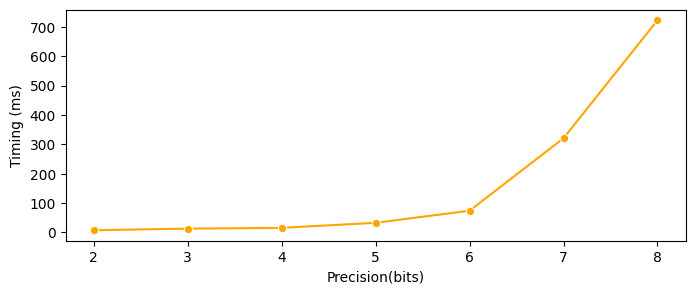
\includegraphics[width=0.8\linewidth]{tex/larger_luts/Figures/timings_pbs_precisions.png}
	\caption{Timings of the PBS with respect to $\log_2(p)$, where $p$ is the plaintext modulus}
	\label{fig:PBS_perfs}
\end{figure}



Intuitively, the reason is simple. When one wants to use a greater $p$, the torus must be sliced into more parts, that are thus smaller. When we switch the modulus to $2N$ in the bootstrapping, the ``windows'' of the accumulator polynomial gets smaller, so the bound on the noise to ensure correct bootstrapping must be smaller. To keep some room to enable the homomorphic capabilities of TFHE, one has to pick a greater value for the degree $N$. As this must be a power of two, it quickly reach values where the polynomial operations gets very slow.

Usually, PBS is not used for plaintext modulus greater than 8 bits. Some constructions exist in the literature to extend the capabilities of this algorithm to larger plaintext spaces, notably the tree bootstrapping of \cite{TCHES:GuiBorAra21} and the WoP-PBS of \cite{AC:CLOT21}. In this thesis, we propose our own in Chapter \ref{chap:larger_lut}.







%!TEX root = ../thesis.tex

\chapter[The Negacyclicity Problem]{Overcoming the Negacyclicity Problem with an Odd Plaintext Modulus}
\label{chap:negacyclicity}


In Section \ref{sec:pbs}, we presented the algorithm of the \gls{PBS}. But we left a question unanswered: what is the actual composition of the accumulator polynomial $\acc$? This is a tricky question, because this definition depends on the countermeasure picked against the negacyclicity problem (that we briefly introduced in Section \ref{sec:overview_blind_rotation}). 


In this chapter, we formalize the negacyclicity problem. We then present the classical countermeasure (the strategy of the padding bit), and our technique of odd plaintext modulus, which is a foundational block for the following contributions presented in this thesis. We finish by going through several others works that propose different countermeasures.


\section{Basics on Negacyclicity}

\paragraph{What is negacyclicity ?}

Let $v(X)$ be a polynomial of the ring $\glweRing$, such that $v(X) = \sum_{k=0}^{N-1} v_k X^k$. Recall how a multiplication by $X$  in this ring ``rotates'' the coefficients of the polynomial: \[X \cdot v(X) = - v_{N - 1} + v_0 \cdot X \dots + v_{N - 2} X^{N - 1}~.\]

In \gls{TFHE}'s blind rotation, the polynomial multiplication is done by the monomial $X^{-\Tilde{\mu}}$, with $\Tilde{\mu} \in \left \lbrace 0, \dots, 2N - 1 \right \rbrace$. This leads to two problems:

\begin{itemize}
	\item A coefficient $v_j$ can be brought in first place by two different rotations: the one induced by the polynomial multiplication by $X^{\modulo{-j}{2N}}$ and the one by $X^{[-j + N]_{2N}}$. It means that two different messages produce the same output.
	\item Each time a coefficient goes last to first, it gets negated (because $X^N = -1$ in the ring). So actually, the multiplication by $X^{[-j]_{2N}}$ yields correctly $v_j$, but the one by $X^{[-j + N]_{2N}}$ yields $-v_j$.
\end{itemize}


As the actual value of $\tilde{\mu}$ is encrypted, this is not possible to predict beforehand whether this undesirable minus sign will appear or not. So a countermeasure needs to be implemented into the scheme to neutralize the negacyclicity problem. The most frequent strategy is to develop encodings for the \gls{LUT} $f$ in the accumulator specifically tailored to handle this issue.


\paragraph{The ``natural'' case.}

Some functions interact naturally very well with the blind rotation algorithm: these are called the \textit{negacyclic functions} and they are presented in Definition \ref{def:negacyclic_function}.


\begin{definition} (Negacyclic Function)
	Let $p$ and $p'$ be two positive integers, with $p$ even. A function $f : \Z_p \mapsto \Z_{p'}$ is negacyclic if and only if it satisfies the following property:
	
	\[
		\forall x \in \Z_p, f\left (\modulo{x + \frac p 2}{p} \right ) = \modulo{-f(x)}{p'}
	\]
	
	\label{def:negacyclic_function}
\end{definition}


With such functions, the accumulator is quite simple to build: intuitively we only fill it with the values of the first half of the torus (so the $f(x)$ with $x \in \left [0, \frac p 2 - 1 \right ]$). So, if we rotate by the value corresponding to $i \ge \frac p 2$, a minus sign appears and we retrieve correctly $-f\left(i - \frac p 2 \right)$ .

We give an explicit formula for this accumulator in Definition \ref{def:negacyclic_accumulator}

\begin{definition} (Negacyclic Accumulator)
		\label{def:negacyclic_accumulator}
		Let $p$ and $p'$ be two positive integers, with $p$ \textbf{even}. Let $f:\Z_p \mapsto \Z_{p'}$ be a negacyclic function. Let $N$ be a power of two. Then, the accumulator $\acc$, defined by:
	
	\[
		\acc^{\textsf{negacyclic}} = X^{\frac{-2N}{2p}} \cdot \sum_{j=0}^{2N / p - 1} X^j \cdot \sum_{i=0}^{p/2 - 1} f(i) X^{i \frac{2N}{p}} \mod (X^N + 1)
	\]
	
\noindent is a valid accumulator for the blind rotation. It means that running the $\BlindRotate$ algorithm with this accumulator yields the right value.
	
	\paragraph{Remark on the encoding:}
	$f(i)$ is an element of the plaintext space $\Z_p$. In the context of this definition, we refer to its encoding into the ciphertext space $\Z_q$ (according to the procedure of Section \ref{sec:encryption}). That is to say, we actually put $\rounding{\frac{f(i) \cdot q}{p}}$ in the coefficients of the polynomial.
\end{definition}



Unfortunately, this construction is merely theoretical. Indeed, in practical setting, restricting the functions to be evaluated by \gls{PBS} only to negacyclic function greatly limits the capability of the scheme. In order to be able to evaluate \textit{any} function in the \gls{PBS}, more sophisticated techniques are required. We introduce the first example of such technique in the next section.


\section{The Classical Countermeasure: the Bit of Padding}
\label{sec:bit_of_padding}

The first countermeasure, that already appeared in the original \gls{TFHE} paper, is called the \textit{bit of padding}. As in the ideal case presented in the previous section, it works in an \textbf{even} plaintext space.

The idea is to ensure that the message stays in the first half of the torus all along the computations. An equivalent way of presenting it is to force the Most Significant Bit (\gls{MSB}) of the message to zero. By doing this, the modswitched phase used as the exponent in the blind rotation $\tilde{\mu}$ lives in $\{0, \dots, N - 1\}$, so the arising minus signs never reach the degree-zero coefficient.

The advantage of this method is that it relaxes the negacyclicity constraint and makes the bootstrapping able to evaluate any function (not only the negacyclic one). However, this construction is rather fragile: any linear function can break it by propagating a carry into the \gls{MSB}. 

To avoid this, when evaluating an homomorphic circuit, the program needs to keep track of the maximal value that each homomorphic operation can yield and make sure that it will never propagate a carry into the \gls{MSB}. This often leads to extra bootstrapping to control the growth of the message and eliminate the overflows. 


In the following, we give the definition of the accumulator $\acc$ in this ``bit-of-padding'' case:

\begin{definition}(Bit-of-Padding accumulator)
	Let $p$ and $p'$ be two positive integers, with $p$ \textbf{even}. Let $f: \Z_p \mapsto \Z_{p'}$ be a function. Let $N$ be a power of two. Then, the accumulator $acc(X)$:
	\[
		\acc^{\textsf{bit-of-padding}} = X^{\frac{-N}{2p}} \cdot \sum_{j=0}^{N / p - 1} X^j \cdot \sum_{i=0}^{p - 1} f(i) X^{i \frac{N}{p}} \mod (X^N + 1)
	\]
	
\noindent is a valid accumulator for the blind rotation.
	\paragraph{Remark on the encoding:}
	Contrary to the purely negacyclic case of Definition \ref{def:negacyclic_accumulator}, $f(i)$ is not encoded in the Most Significant Bits of the polynomial's coefficient. Instead, the \gls{MSB} is reserved and fixed to zero to maintain the encoded value in the first half of the torus. That is to say, we actually put $\rounding{\frac{f(i) \cdot q}{2 \cdot p}}$ in the coefficients of the polynomial.
\end{definition}


An example of such an accumulator is shown on Figure \ref{fig:negacyclic_accumulator}.

\begin{figure}[H]
	\centering
	\begin{tikzpicture}
		\drawHalfRing{4}{small}{true}{true}{true}
		\drawSingleRingHalfColor{64}{4}{big}{true}{false}{true}
	\end{tikzpicture}
				
	\vspace{1.5em}
	
	\textbf{Bit-of-Padding Accumulator:}\\[0.5em]
	\negacyclicAccumulator{4}{32}
	
	\caption{An example of bit-of-padding accumulator, with $p=4$ and $N = 32$. Hatching shows the parts which have an additional minus signs.}
	\label{fig:negacyclic_accumulator}
\end{figure}





The drawback of the bit-of-padding padding makes very challenging the development of homomorphic applications, because it prevents to use the linear operations freely. One should keep track of the maximal value contained in a ciphertext to avoid an overflow that would fill the padding bit. In Chapter \ref{chap:p_encodings}, we will demonstrate how this method makes the evaluation of Boolean circuit very inefficient, and we propose a new method that improves it.

Other constructions have been developed to avoid these drawbacks, we present them in Section \ref{sec:soa_padding_bit}.



\section{Other Countermeasures Avoiding the Bit of Padding}
\label{sec:soa_padding_bit}

Because the classical bit-of-padding solution brings too many constraints on the evaluation of computational circuits, several alternative constructions have been proposed to homomorphiclaly evaluate \gls{LUT}. To do so, many of these constructions adopt a similar strategy: they decompose the target function into a sequence of several \gls{PBS} steps. 

A notable line of work, including \cite{EPRINT:YXSCZ21}, \cite{AC:LiuMicPol22}, and \cite{TCHES:KluSch23}, employs a two-step \gls{PBS} strategy. In these approaches, the first \gls{PBS} evaluates a quantity  encrypting the bit indicating whether the message lies in the positive or negative half of the torus. This effectively extracts the ``sign'' of the message. The second \gls{PBS} then evaluates the actual function of interest regardless of the effects of negacyclicity, producing a result that may be flipped in sign. The ambiguity introduced by this flip is corrected using the result of the first \gls{PBS}. While the specific techniques used to perform this correction vary across works, the overall architecture remains the same: use the first \gls{PBS} to identify the torus half, and use this information to rectify the sign of the second \gls{PBS} output.

Another interesting approach is presented in \cite{AFRICACRYPT:CBSZ23}, where the target function is expressed as a sum of functions sharing a particular structure: so-called \textit{pseudo-odd} and a \textit{pseudo-even} function. These two properties are special cases of negacyclic functions, so they allow an evaluation with a \gls{PBS} without suffering from the negacyclicity issue. Although this decomposition may require more than two \gls{PBS} calls, an important advantage of the method is that the evaluations can be carried out in parallel. This contrasts with the previously mentioned approaches, which are intrinsically sequential due to the dependency between the two \gls{PBS} stages.

A completely different line of work is explored in \cite{AC:CLOT21}, which introduces the “Without-Padding \gls{PBS}” (WoP-\gls{PBS}) construction. A more refined version of this technique is presented in \cite{JC:BBBCLO23}, and we describe it here. The method begins by evaluating a scaled sign function (that is inherently negacyclic) using a standard \gls{PBS}. Following this, the individual bits of the message are extracted and converted into $\GGSW$ ciphertexts (see Definitions \ref{def:ggsw} and \ref{def:ggsw2}) using a procedure known as \textit{circuit bootstrapping}. These ciphertexts are then used as selectors in a graph of $\CMUX$ operations (Definition \ref{def:cmux}) to select an appropriate accumulator based on the high-order bits of the message. Finally, a traditional \gls{PBS} is used to rotate the selected accumulator according to the remaining lower-order bits.

Although this technique is slower for small plaintext sizes, it scales particularly well with an increasing plaintext sizes. Notably, it enables the homomorphic evaluation of LUTs with larger plaintext sizes beyond what is feasible with classical \gls{PBS} techniques, up to approximately 20 input bits.


In this thesis, we focus on a method we introduced in \cite{TCHES:BonPoiRiv24}: \textit{the odd plaintext modulus}.

\section{Our Contribution: the Odd Plaintext Modulus}
\label{sec:odd_modulus}

Negacyclicity has a quite different effect depending of the parity of the plaintext modulus $p$. Recall that $\mu = m + e \in \Z_q$, with $e$ sampled from a small centered Gaussian. Because the error is small, $\mu$ does not take all the values of $\Z_q$ with the same probability: in particular, the densest parts in terms of probability over $\Z_q$ are the one close to the ``noiseless'' encodings of $m$, namely $\left \{ \rounding{\frac {k q}{p}} ~\middle |~ k \in \Z_p \right \}$. We illustrate this distribution on Figure \ref{fig:density_of_phase}. We call these sections of the torus the \emph{dense spots}.


\begin{figure}[h]
	\centering
	\begin{minipage}{0.47\textwidth}
		\centering
		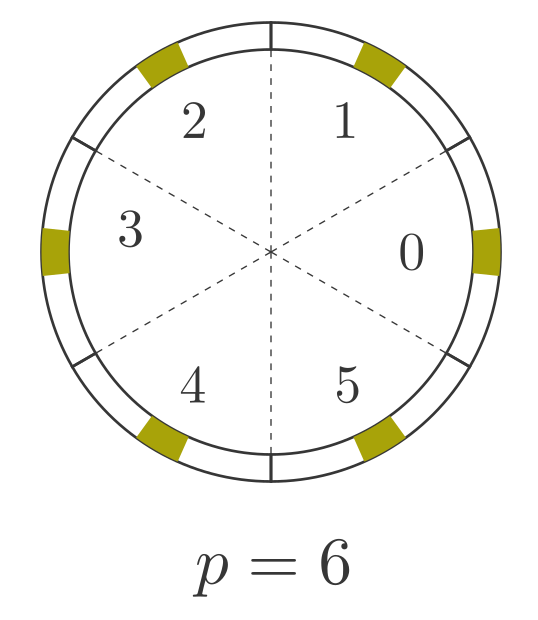
\includegraphics[width=0.8\textwidth]{img/to_harmonize/busy_sectors_2.png}
	\end{minipage}
	\hspace{0.04\textwidth}
	\begin{minipage}{0.47\textwidth}
		\centering
		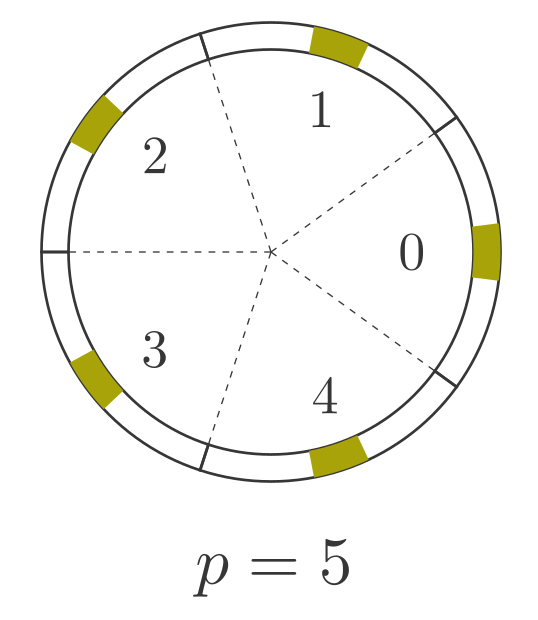
\includegraphics[width=0.8\textwidth]{img/to_harmonize/busy_sectors.png}
	\end{minipage}
	\caption{Distribution of the values of $\mu$ across $\mathbb{Z}_q$ for $p = 6$ and $p = 5$: the colored parts show the dense spots where the value has a high probability to lie in. The width of these sectors depends on $\sigma$ (the standard deviation of the error distribution $\chi$ of \gls{TFHE}). Note that this repartition looks similar for $\Tilde{\mu}$ in $\mathbb{Z}_{2N}$.}
	\label{fig:density_of_phase}
\end{figure}


When we transpose these dense spots into $\Z_{2N}$, they become the sectors close to $\left \{ \rounding{\frac{k \cdot 2N}{p}} \mid k \in \Z_p \right \}$. 

Let $k \in \Z_p$, the multiplication $X^{- \frac{k \cdot 2N}{p}} \cdot v(X)$ in the ring $\glweRing$ yields the same degree-zero coefficient as the multiplication  $X^{\modulo{- \frac{k \cdot 2N}{p} + N}{2N}} \cdot v(X)$, up to the minus sign. To make the rest of this section clearer, we change a bit the writing of the exponent as such: 
\[\modulo{
	\frac{
		-k \cdot 2N
	}
	{
		p
	}
	+ N
}{2N} = 
\modulo{
	\frac{
		(-k + \frac p 2 ) \cdot 2N
	}
	{p}
}
{2N}\]


This is where the parity of $p$ plays a part: if $p$ is even, then $\modulo{
	\frac{
		(-k + \frac p 2 ) \cdot 2N
	}
	{p}
}
{2N}$ is a dense spot as well. So collisions happen with high probability.  On the other hand, let us consider an odd value for $p$. Then, $\modulo{
	\frac{
		(-k + \frac p 2 ) \cdot 2N
	}
	{p}
}{2N}$ is no longer a dense spot, as it lies exactly halfway between the two dense spots $\modulo{
	\frac{
		(-k + \frac {p-1} {2} ) \cdot 2N
	}
	{p}
}{2N}$ and $\modulo{
	\frac{
		(-k + \frac {p+1} {2} ) \cdot 2N
	}
	{p}
}{2N}$. As a consequence, collisions never occur. Figure \ref{fig:torus_p_even_vs_odd} illustrates this phenomenon.


\begin{figure}
	\begin{subfigure}{0.49\linewidth}
		    \centering
		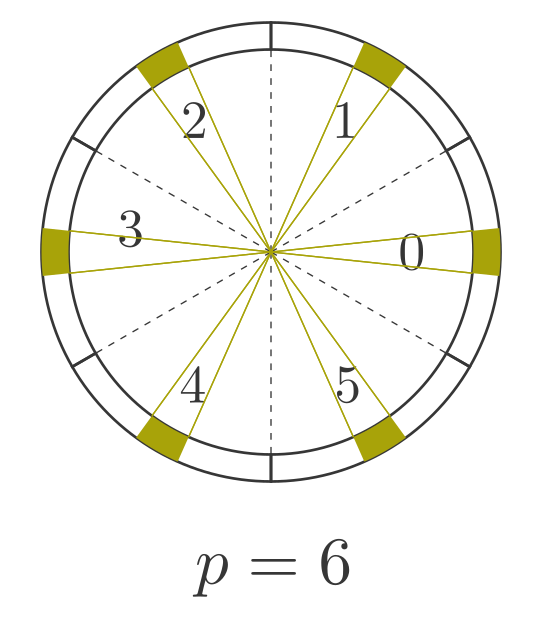
\includegraphics[width=0.5\linewidth]{img/to_harmonize/torus_p_even.png}
		\caption{With $p$ even, the dense spots of each half of the torus are aligned.}
		\label{fig:torus_p_even}
	\end{subfigure}\hspace{1em}% Adjust the margin width as needed
	\begin{subfigure}{0.49\linewidth}
		\centering
		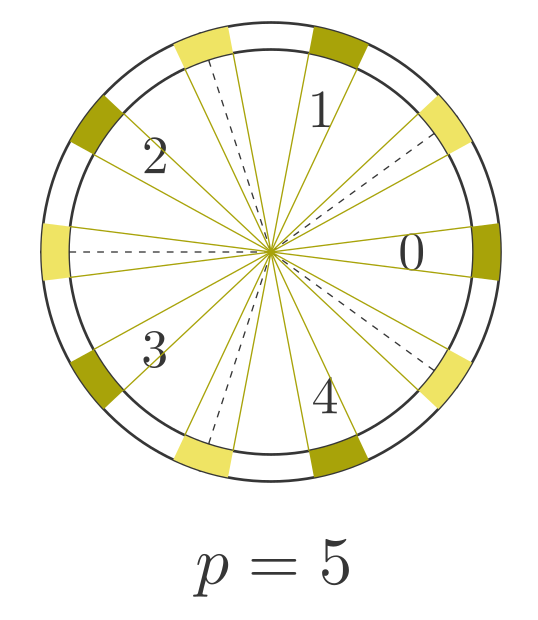
\includegraphics[width=0.5\linewidth]{img/to_harmonize/torus_p_odd.png}
		\caption{With $p$ odd, the dense spots face empty spots, close to the bounds of the $p$-sectors.}
	\end{subfigure}
	\caption{}
	\label{fig:torus_p_even_vs_odd}
\end{figure}



So, by selecting odd values for the plaintext modulus, the negacyclicity problem is naturally neutralized.


We present in Definition \ref{def:odd_accumulator} the formula for the accumulator in this case. Note that because $N$ is a power of two and $p$ an odd value, some rounding is required in the quotient $\frac N p$, but we omit it to keep notations lighter, (or equivalently, the division operator is assumed to include rounding).

\begin{definition}(Odd-case Accumulator)
	\label{def:odd_accumulator}
	Let $p$ and $p'$ be two integers, with $p$ \textbf{odd}. Let $f: \Z_p \mapsto \Z_{p'}$ a function, and $N$ a power of two. Then, the accumulator $\acc \in \glweRing$ has the form:
	\[
		\acc^{\textsf{odd-modulus}} = X^{- \frac {N} {2p}} \cdot \sum_{j=0}^{N/p - 1} X^j  \cdot \left ( \sum_{i=0}^{\frac{p-1}{2}} f(i) X^{i \frac{2N}{p}} + \sum_{i=0}^{\frac{p-1}{2} - 1} -f \left (i + \frac{p+1}{2} \right ) X^{i \frac{2N}{p} + \frac N p} \right )
	\]
	
	\paragraph{Remark on the encoding:}
	With this construction, we do not need a bit of padding anymore. So, the values $f(i)$ are encoded using the simple encoding of Section \ref{sec:encryption}, that is to say $\rounding{\frac{f(i) \cdot q}{p}}$.
\end{definition}



Let us explain the structure of this accumulator. The polynomial has degree $N$ and is made of $p$ distinct windows of width $\frac{N}{p}$. Each of these windows has constant coefficient value $f(k)$, for $k \in \{0, \dots, p-1\}$.
For $0 \le \alpha \le \frac{p-1}{2}$, the range of degrees whose coefficients are $f(\alpha)$ is $\left [ \alpha \frac{2N}{p} - \frac{N}{2p}~;~ \alpha \frac{2N}{p} + \frac{N}{2p} \right ]$. Now, for $\frac{p+1}{2} \le \beta \le p-1$, we can write $\beta = \alpha + \frac{p+1}{2}$, with $0 \le \alpha < \frac{p-1}{2}$. This time, the range of spanned degrees is $\left [ \alpha \frac{2N}{p} + \frac{N}{2p} ~;~ (\alpha + 1) \frac{2N}{p} - \frac{N}{2p} \right ]$. Thus, the values $k \in \{0, \dots, p-1\}$ spans the entire space $[0; N)$ without overlap. The values over $\frac{p+1}{2}$ gets negated by the negacyclicity, so the underlying coefficient is also negated to compensate this effect. We illustrate this construction on Figure \ref{fig:accumulator_odd}.




\begin{figure}[H]
	\centering
	
\begin{tikzpicture}
		\drawSingleRing{5}{5}{small}{true}{true}{true}
		\drawRingOddEncoding{64}{5}{big}{true}{false}
		\draw[red, loosely dashed, line width=1mm] (-6,0) -- (6,0);
	\end{tikzpicture}
	
	\vspace{1.5em}
%	
	\textbf{Odd-Modulus Accumulator:}\\[0.5em]
	\oddAccumulator{5}{32}
%	
%	\vspace{1.5em}
%	\textbf{Rotated by $N$:}\\
%	\oddAccumulatorInverted{5}{32}
	\caption{Illustration of the construction of the Odd-Modulus accumulator. On top is the ring $\Z_{2N}$ splitted in windows. Below is a representation of the polynomial $v$, with its version once rotated by a multiplication by $X^N$. On the figure, $p = 5$ and $N = 32$. Hatching shows the parts which have an additional minus signs}
	\label{fig:accumulator_odd}
\end{figure}


If we compare this approach to the bit-of-padding one, the windows have half the size. So we may think that the bound on the maximal noise to ensure correctness must be twice tighter. However, because the bit-of-padding accumulator makes use of only one half of the torus, the windows actually have the same width if we consider the same size of plaintext space. In Section \ref{sec:parametrization}, we elaborate further on how the parametrization of the scheme is handled in this case.


With this technique, no bit of padding is required. Consequently, it allows to use the linear homomorphisms without worrying about carry propagation. This is a key improvement that is at the root of the works presented in the rest of this thesis.





\section{Conclusion}

Our idea of employing odd plaintext moduli that we developed in Section \ref{sec:odd_modulus} do not have any computational overhead with respect to the classical bit-of-padding technique of Section \ref{sec:bit_of_padding}, while removing all the constraints the latter put on the homomorphic compilation. This is not the case of the other methods of the state of the art that we summed up in Section \ref{sec:soa_padding_bit}, which all increase the amount of computation 

However, working with an odd modulus may seem unhandy: data types in programming are usually defined on a power-of-two modulus for example. But we show in the following chapters (Chapter \ref{chap:p_encodings}, \ref{chap:hyppogriph}, \ref{chap:transistor} and \ref{chap:larger_lut}) that this introduces new applications and homomorphic capabilities to \gls{TFHE}.



% Chapter on Boolean Functions
% !TeX_ROOT=../../thesis.tex

%%%% 2. PACKAGES %%%%
%\usepackage{subcaption}
%\usepackage{multirow}
%\usepackage{todonotes}
%\usepackage{wrapfig}
%\usepackage{tikz}

%%% Custom header %%%
%%!TEX root=../main.tex

% Packages
%

\usepackage[utf8]{inputenc}
\usepackage[T1]{fontenc}
\usepackage{hyperref}
\usepackage{verbatim}
\usepackage{tikz}
\usetikzlibrary{positioning,calc}
\usepackage{xspace}
\usepackage{amsmath} %\usepackage{amsthm}
\usepackage{amssymb}
\usepackage{mathtools}
\usepackage{pifont}
\usepackage{etoolbox}
\usepackage[normalem]{ulem}
\usepackage{booktabs}
\usepackage{array}
\usepackage{cite}
\usepackage{multibib}
\usepackage{url}
\usepackage{algorithm}
\usepackage{algpseudocode}
\usepackage{paralist}
\usepackage{mathrsfs}
\usepackage{relsize}
\usepackage{stmaryrd}
\usepackage[lambda,n,operators]{cryptocode}

\newtoggle{notes}
\toggletrue{notes} % set to false to remove colored notes from the paper

%--------------------------------------------------------
% Editorial
%--------------------------------------------------------

\newcommand{\redunderline}[1]{\textcolor{red}{\underline{\textcolor{black}{#1}}}} 
\newcommand{\TBW}{\textcolor{blue}{\textbf{To Be Written...}}}
\newcommand{\Note}[1]{\textcolor{magenta}{ $\langle \! \langle$ #1 $\rangle \! \rangle$}}
\newcommand{\todonote}[1]{\todo[inline]{MyName: #1}}

%--------------------------------------------------------
% General notations
%--------------------------------------------------------

\let\vec\mathbf
\newcommand{\bit}{\ensuremath{\{0,1\}}\xspace}
\newcommand{\getsr}{\leftarrow_{r}}
\newcommand{\poly}{\ensuremath{\mathsf{poly}}\xspace}

%--------------------------------------------------------
% Standard proba, games, proofs, sampling, distributions
%--------------------------------------------------------

\newcommand{\Good}{\ensuremath{\mathsf{Good}}\xspace}
\newcommand{\Bad}{\ensuremath{\mathsf{Bad}}\xspace}
\newcommand{\equivStat}{\ensuremath{\overset{\mathsf{stat}}{\equiv}}\xspace}
\newcommand{\equivComp}{\ensuremath{\overset{\mathsf{comp}}{\equiv}}\xspace}
\newcommand{\view}{\ensuremath{\textsc{View}}\xspace}
\newcommand{\state}{\ensuremath{\mathsf{st}}\xspace}
\newcommand{\st}{\state}
\newcommand{\Hyb}{\ensuremath{\mathsf{Hyb}}\xspace}
\newcommand{\Exp}{\ensuremath{\mathsf{Exp}}\xspace}
\newcommand{\myGame}{\ensuremath{\mathsf{Game}}\xspace}
\newcommand{\Event}{\ensuremath{\mathsf{E}}\xspace}
\newcommand{\Span}{\ensuremath{\mathsf{Span}}}
\newcommand{\prob}[1]{{\Pr}\left[\,{#1}\,\right]}
\newcommand{\probb}[2]{{\Pr}_{#1}\left[\,{#2}\,\right]}
\newcommand{\Dx}{\mathcal{D}}
\newcommand{\Hx}{\mathcal{H}}
\newcommand{\Sx}{\mathcal{S}}
\newcommand{\Lx}{\mathcal{L}}
\newcommand{\Dist}{\mathcal{D}}
\newcommand{\Expect}{\ensuremath{\mathbb{E}}\xspace}
\newcommand{\Sample}{\ensuremath{\mathsf{Sample}}\xspace}
\newcommand{\Sim}{\ensuremath{\mathsf{Sim}}\xspace}

%--------------------------------------------------------
% Adversaries, oracles
%--------------------------------------------------------

\newcommand{\AdvA}{\ensuremath{\mathcal{A}}\xspace}
\newcommand{\AdvB}{\ensuremath{\mathcal{B}}\xspace}
\newcommand{\AdvC}{\ensuremath{\mathcal{C}}\xspace}
\newcommand{\AdvD}{\ensuremath{\mathcal{D}}\xspace}

\newcommand{\adv}{\ensuremath{\mathsf{Adv}}\xspace}
\newcommand{\oracle}{\ensuremath{\mathcal{O}}\xspace}

%--------------------------------------------------------
% Classes, sets, groups
%--------------------------------------------------------

\newcommand{\BPP}{\ensuremath{\mathsf{BPP}}\xspace}
\newcommand{\NP}{\ensuremath{\mathsf{NP}}\xspace}
\newcommand{\coNP}{\ensuremath{\mathsf{coNP}}\xspace}
\newcommand{\PSPACE}{\ensuremath{\mathsf{PSPACE}}\xspace}
\newcommand{\NC}{\ensuremath{\mathsf{NC}}\xspace}

\newcommand{\Z}{\mathbb{Z}}
\newcommand{\F}{\mathbb{F}}
\newcommand{\N}{\mathbb{N}}
\newcommand{\R}{\mathbb{R}}
\newcommand{\G}{\mathbb{G}}
\newcommand{\Gt}{\mathbb{G}_{\mathsf{T}}}
\newcommand{\Hset}{\mathbb{H}}
\newcommand{\Zn}{\mathbb{Z}_n}
\newcommand{\Group}{\mathbb{G}}

\newcommand{\Lang}{\ensuremath{\mathscr{L}}}
\newcommand{\Lpar}{\ensuremath{\Lang_{\param}}\xspace}
\newcommand{\setX}{\mathcal{X}}
\newcommand{\setY}{\mathcal{Y}}
\newcommand{\keyspace}{\mathcal{K}}


%--------------------------------------------------------
% Primitives, algorithms
%--------------------------------------------------------

\newcommand{\proverS}{\ensuremath{\mathsf{P}_{\Sigma}}\xspace}
\newcommand{\verifierS}{\ensuremath{\mathsf{V}_{\Sigma}}\xspace}
\newcommand{\prover}{\ensuremath{\mathsf{P}}\xspace}
\newcommand{\verifier}{\ensuremath{\mathsf{V}}\xspace}
\newcommand{\sender}{\ensuremath{\mathsf{S}}\xspace}
\newcommand{\receiver}{\ensuremath{\mathsf{R}}\xspace}
\newcommand{\ZK}{\textsf{ZK}\xspace}
\newcommand{\zk}{\textsf{zk}\xspace}
\newcommand{\HVZK}{\textsf{HVZK}\xspace}
\newcommand{\NIZK}{\hardprobfont{NIZK}\xspace}
\newcommand{\NIZKs}{\hardprobfont{NIZKs}\xspace}
\newcommand{\NIWI}{\hardprobfont{NIWI}\xspace}
\newcommand{\sigmap}{$\Sigma$-protocol\xspace}
\newcommand{\sigmaps}{$\Sigma$-protocols\xspace}
\newcommand{\OT}{\ensuremath{\mathsf{OT}}\xspace}
\newcommand{\OTs}{\ensuremath{\mathsf{OTs}}\xspace}
\newcommand{\Eval}{\ensuremath{\mathsf{Eval}}\xspace}
\newcommand{\PRG}{\ensuremath{\mathsf{PRG}}\xspace}
\newcommand{\Hash}{\ensuremath{\mathsf{H}}\xspace}
\newcommand{\Setup}{\ensuremath{\mathsf{Setup}}\xspace}
\newcommand{\GroupGen}{\textsf{BilinearGen}\xspace}
\newcommand{\DDHGen}{\textsf{DHGen}\xspace}
\newcommand{\PGen}{\textsf{PGen}\xspace}
\newcommand{\KeyGen}{\ensuremath{\mathsf{KeyGen}}\xspace}
\newcommand{\Enc}{\ensuremath{\mathsf{Enc}}\xspace}
\newcommand{\Dec}{\ensuremath{\mathsf{Dec}}\xspace}
\newcommand{\INDCCA}{\ensuremath{\mathsf{IND\text{-}CCA}}\xspace}
\newcommand{\INDCPA}{\ensuremath{\mathsf{IND\text{-}CPA}}\xspace}
\newcommand{\Rand}{\ensuremath{\mathsf{Rand}}\xspace}
\newcommand{\com}{\ensuremath{\mathsf{com}}\xspace}
\newcommand{\Commit}{\ensuremath{\mathsf{Commit}}\xspace}
\newcommand{\Prove}{\ensuremath{\mathsf{Prove}}\xspace}
\newcommand{\prove}{\ensuremath{\mathsf{prove}}\xspace}
\newcommand{\Verify}{\ensuremath{\mathsf{Verify}}\xspace}
\newcommand{\Answer}{\ensuremath{\mathsf{Answer}}\xspace}
\newcommand{\Open}{\ensuremath{\mathsf{Open}}\xspace}
\newcommand{\myproof}{\ensuremath{\vec{\pi}}\xspace}
\newcommand{\Gen}{\ensuremath{\mathsf{Setup}}\xspace}
\newcommand{\KGen}{\ensuremath{\mathsf{KeyGen}}\xspace}
\newcommand{\Equivocate}{\ensuremath{\mathsf{Equivocate}}\xspace}
\newcommand{\SimSetup}{\ensuremath{\mathsf{SimSetup}}\xspace}
\newcommand{\Stretch}{\ensuremath{\mathsf{Stretch}}\xspace}
\newcommand{\Trapdoor}{\ensuremath{\mathsf{Trapdoor}}\xspace}

\newcommand{\pk}{\ensuremath{\mathsf{pk}}\xspace}
\newcommand{\sk}{\ensuremath{\mathsf{sk}}\xspace}
\newcommand{\ek}{\ensuremath{\mathsf{ek}}\xspace}
\newcommand{\vk}{\ensuremath{\mathsf{vk}}\xspace}
\newcommand{\pvk}{\ensuremath{\mathsf{pvk}}\xspace}
\newcommand{\PVK}{\ensuremath{\mathsf{PVK}}\xspace}
\newcommand{\hk}{\ensuremath{\mathsf{hk}}\xspace}
\newcommand{\aux}{\ensuremath{{\mathsf{aux}}}\xspace}
\newcommand{\crs}{\ensuremath{{\mathsf{crs}}}\xspace}
\newcommand{\param}{\ensuremath{{\mathsf{par}}}\xspace}
\newcommand{\trap}{\ensuremath{\mathcal{T}}\xspace}
\newcommand{\eps}{\varepsilon}

%--------------------------------------------------------
% Hard problems
%--------------------------------------------------------

\newcommand{\hardprobfont}[1]{\texorpdfstring{\ensuremath{\textsf{#1}}}{#1}}
\newcommand{\kLIN}{\ensuremath{k\text{-}\mathsf{Lin}}\xspace}
\newcommand{\SEDL}{\hardprobfont{SEDL}\xspace}
\newcommand{\DL}{\hardprobfont{DL}\xspace}
\newcommand{\DDH}{\hardprobfont{DDH}\xspace}
\newcommand{\kerDH}{\hardprobfont{kerDH}\xspace}
\newcommand{\kernel}{\mathsf{ker}\xspace}
\newcommand{\DHP}{\hardprobfont{DH}\xspace}
\newcommand{\DLin}{\hardprobfont{DLin}\xspace}
\newcommand{\XDH}{\hardprobfont{XDH}\xspace}
\newcommand{\CDH}{\hardprobfont{CDH}\xspace}
\newcommand{\LWE}{\hardprobfont{LWE}\xspace}
\newcommand{\RLWE}{\hardprobfont{RLWE}\xspace}
\newcommand{\GLWE}{\hardprobfont{GLWE}\xspace}

\newcommand{\SXDH}{\hardprobfont{SXDH}\xspace}
\newcommand{\DCR}{\hardprobfont{DCR}\xspace}
\newcommand{\dlog}{\ensuremath{\mathsf{dlog}}\xspace}

%--------------------------------------------------------
% Various
%--------------------------------------------------------

\newcommand{\map}{\ensuremath{\mathsf{map}}\xspace}
\newcommand{\mode}{\mathsf{mode}}
\newcommand{\token}{\ensuremath{\mathsf{token}}\xspace}
\newcommand{\seed}{\ensuremath{\mathsf{seed}}\xspace}
\newcommand{\inp}{\ensuremath{\mathsf{in}}\xspace}
\newcommand{\outp}{\ensuremath{\mathsf{out}}\xspace}
\newcommand{\circuit}{\ensuremath{\mathcal{C}}\xspace}
\newcommand{\size}[1]{\ensuremath{\left\vert #1 \right\vert}\xspace}
\newcommand{\myand}{\ensuremath{\mathsf{and}}\xspace}
\newcommand{\myxor}{\ensuremath{\mathsf{xor}}\xspace}
\newcommand{\xor}{\mathbin{\mathsf{xor}}}
\newcommand{\mynot}{\ensuremath{\mathsf{not}}\xspace}
\newcommand{\Input}{\ensuremath{\mathsf{Input}}\xspace}
\newcommand{\pp}{\ensuremath{\mathsf{pp}}\xspace}


%--------------------------------------------------------
% Double angle brackets
%--------------------------------------------------------

\makeatletter
\DeclareFontFamily{OMX}{MnSymbolE}{}
\DeclareSymbolFont{MnLargeSymbols}{OMX}{MnSymbolE}{m}{n}
\SetSymbolFont{MnLargeSymbols}{bold}{OMX}{MnSymbolE}{b}{n}
\DeclareFontShape{OMX}{MnSymbolE}{m}{n}{
    <-6>  MnSymbolE5
   <6-7>  MnSymbolE6
   <7-8>  MnSymbolE7
   <8-9>  MnSymbolE8
   <9-10> MnSymbolE9
  <10-12> MnSymbolE10
  <12->   MnSymbolE12
}{}
\DeclareFontShape{OMX}{MnSymbolE}{b}{n}{
    <-6>  MnSymbolE-Bold5
   <6-7>  MnSymbolE-Bold6
   <7-8>  MnSymbolE-Bold7
   <8-9>  MnSymbolE-Bold8
   <9-10> MnSymbolE-Bold9
  <10-12> MnSymbolE-Bold10
  <12->   MnSymbolE-Bold12
}{}

\let\llangle\@undefined
\let\rrangle\@undefined
\DeclareMathDelimiter{\llangle}{\mathopen}%
                     {MnLargeSymbols}{'164}{MnLargeSymbols}{'164}
\DeclareMathDelimiter{\rrangle}{\mathclose}%
                     {MnLargeSymbols}{'171}{MnLargeSymbols}{'171}
\makeatother

%%% Local Variables:
%%% mode: latex
%%% TeX-master: "../main"
%%% End:







%%%%% 7. PAPER CONTENT %%%%
%\newcommand{\T}{\mathbb{T}}
\newcommand{\B}{\mathbb{B}}
\newcommand{\drawfrom}{\overset{\$}{\leftarrow}}
\newcommand{\rounding}[1]{\left \lfloor #1 \right \rceil}
\newcommand{\modulo}[2]{\left [ #1 \right ]_{#2}}
\newcommand{\customnorm}[1]{\left \lVert #1 \right \rVert}

\newcommand{\Encoding}{\mathcal{E}}
\newcommand{\EncDef}[2]{\begin{cases} 0 \mapsto #1 \\ 1 \mapsto #2 \end{cases}}
\newcommand{\EncDefZero}[1]{\begin{cases} 0 \mapsto #1 \\ 1 \mapsto \{0\} \end{cases}}
\newcommand{\EncDefOne}[1]{\begin{cases} 0 \mapsto \{0\} \\ 1 \mapsto \{#1\} \end{cases}}

\newcommand{\GroupP}{\langle \mathbb Z_p ; + \rangle}

% commentaires
\def\TODO#1{\todo[inline, color=orange!30]{\textbf{TODO:} #1}}
\def\MR#1{\todo[inline, color=blue!15]{\textbf{Matthieu:} #1}}
\def\DP#1{\todo[inline, color=red!15]{\textbf{David:} #1}}
\def\NB#1{\todo[inline, color=yellow!15]{\textbf{Nicolas:} #1}}

%% !TeX_ROOT=../../thesis.tex


\gls{TFHE} being the most efficient scheme to handle data of small precision, it is a natural choice when it comes to evaluate homomorphically Boolean circuits. However, performances of the existing frameworks are still limited. 

The most straightforward method, already introduced in the original \gls{TFHE} paper \cite{JC:CGGI20} under the name \emph{gate bootstrapping}, consists in running one bootstrapping for each bivariate Boolean gate of the circuit. As a consequence, the conversion of the original Boolean circuit in a homomorphic circuit handling encrypted bits is straightforward, moreover the noise growth is contained thanks to the systematic use of bootstrapping. However, this approach is very expensive due to the high numbers of bootstrappings and makes it quite suboptimal for large circuits.


In this chapter, we introduce a new framework to homomorphically evaluate Boolean functions on encrypted data efficiently, i.e. by reducing the amount of necessary bootstrappings. Our approach introduces an \emph{intermediate homomorphic layer} which encodes the bits (elements of $\Z_2$) on a small ring $\Z_p$ before encrypting them. This allows us to evaluate Boolean functions with one cheap homomorphic sum followed by one bootstrapping. After formalizing the underlying concept of $p$-\emph{encoding} and explaining our evaluation strategy, we investigate the issue of finding valid sets of encodings for a Boolean function. We characterize this problem and provide an exact constructive algorithm to solve it. We further provide a sieving heuristic finding solutions more efficiently but at the cost of loosing optimally. Since our method is only efficient for Boolean functions with limited number of inputs, we also propose a heuristic to decompose any Boolean circuit into Boolean functions which are efficiently evaluable using our approach. Finally, we apply our technique to various cryptographic primitives, namely the SIMON block cipher, the Trivium stream cipher, the Keccak permutation, the Ascon S-box and the \gls{AES} S-box. Compared to previous works implementing the same primitives (for SIMON, Trivium and \gls{AES}) our implementations achieve significant speedups.

After some technical preliminaries on Boolean circuits (Section \ref{sec:p_encodings_preliminaries_boolean}), we introduce a new concept of \emph{intermediate homomorphic layer} and explain how bits are encoded  in Section \ref{sec:p_encodings_homorphic_layer} and the algorithms to construct it in Sections \ref{sec:p_encodings_search} and \ref{sec:p_encodings_graphs}. Finally, we describe some implementation works in Section \ref{sec:p_encodings_TFHE_adaptation} and our experimental results in Section \ref{sec:p_encodings_implementations}.











%\section{Preliminaries on Boolean Functions and Boolean Circuits}
\label{sec:p_encodings_preliminaries_boolean}


A Boolean function has the form $f: \B^\ell \longrightarrow \B$, with $\ell$ being called the \emph{arity} of the function. 

\begin{definition}
    
The Algebraic Normal Form (ANF) of a Boolean function $f: \{0,1\}^\ell \mapsto \{0,1\}$ is a polynomial expression in which each term corresponds to a specific input combination of $n$ variables. The ANF is defined as follows: \[f(x_1, x_2, \ldots, x_l) = a_0 \oplus a_1x_1 \oplus a_2x_2 \oplus \ldots \oplus a_{2^n-1}x_1x_2\ldots x_l\] \begin{align*}
\text{where: }a_0, a_1, a_2, \ldots, a_{2^\ell-1} & \in \{0,1\} \quad \text{are the Boolean coefficients and} \\
x_1, x_2, \ldots, x_\ell & \quad \text{are called the Boolean variables}
\end{align*}
\end{definition}

This result means that any Boolean function can be evaluated by the means of \texttt{AND} and \texttt{XOR} operations. In the following, we will focus on the implementation of Boolean circuits composed of these operations exclusively.


A Boolean function can be represented by its \emph{truth table}, which is simply a table gathering all the possible inputs and the corresponding result of the application by the function. It can also be represented with a Boolean formula. A third representation is the \emph{Boolean circuit}:

\begin{definition}
    A Boolean circuit associated to the Boolean function $f$ is a finite Directed Acyclic Graph whose edges are \emph{wires} and vertices are \emph{Boolean gates} representing Boolean operations. We consider \texttt{AND} gates and \texttt{XOR} gates, of fan-in 2 and fan-out 1. We also consider copy gates, of fan-in 1 and fan-out $>1$, that outputs several copies of its input. A circuit is further formally composed of input gates of fan-in 0 and fan-out 1, and output gates of fan-in 1 and fan-out 0.
    
    Evaluating a $\ell$-input $m$-output circuit consists in writing an input $\vec{x} \in \B^\ell$ in the input gates, processing the gates from input gates to output gates, then reading the outputs from the output gates.

\end{definition}


This notion of Boolean circuit will be particularly useful in Section \ref{sec:p_encodings_graphs}.


%\section{Boolean Encoding over $\Z_p$ and Homomorphic Evaluation Strategy Between $\B$ and $\Z_p$}
\label{sec:p_encodings_homorphic_layer}



We propose a construction in which we embed Boolean values in $\Z_p$ for well-chosen values of $p$, forming an ``intermediate homomorphic layer'' between $\B$ (the plaintext space of bits) and $\Z_q$ (the ciphertext space). In the following, we explain how we define such a layer, and we describe our new strategy to evaluate Boolean functions in a more efficient way without considering the circuit representation of the function. Note that we generalize this construction to arithmetic spaces in Chapter \ref{chap:hyppogriph}.


\subsection{Encoding of $\B$ over $\Z_p$}

To represent Boolean values over $\Z_p$, we use a mapping function that we call a \emph{$p$-encoding}:

\begin{definition}[$p$-encoding]
    A \emph{$p$-encoding} is a function $\Encoding: \B \mapsto 2^{\Z_p}$ that maps the Boolean space to a subset of the discretized torus. A $p$-encoding is \emph{valid} if and only if:
    \begin{equation}
        \begin{cases}
            \Encoding(0) \cap \Encoding(1) = \emptyset~\text{ and}\\
            \text{if $p$ is even:} ~\forall \:x \in \mathbb Z_p, \forall \:b \in \B: x \in \Encoding(b) \iff \left [ x + \frac p 2 \right ]_p \notin \Encoding(b)
        \end{cases}
    \label{def:validity}
    \end{equation}
    We call this last property \emph{relaxed negacyclicity}.
    \label{def:encoding}
\end{definition}



\begin{figure}[ht]
	\centering
	\begin{minipage}{0.45\textwidth}
		\centering
		\begin{tikzpicture}[scale=0.8]
			\drawSingleRingGreenRed{15}{small}{true}{true}{9, 10}{0, 8, 11, 12, 14}
		\end{tikzpicture}
		\caption*{Example with $p=15$}
	\end{minipage}
	\hfill
	\begin{minipage}{0.45\textwidth}
		\centering
		\begin{tikzpicture}[scale=0.8]
			\drawSingleRingGreenRed{16}{small}{true}{true}{8, 12, 13}{0, 4, 9, 11}
		\end{tikzpicture}
		\caption*{Example with $p=16$}
	\end{minipage}
	
	\caption{Representation of two valid $p$-encodings. The green part represents $\Encoding(1)$,  and the red part $\Encoding(0)$. Note that even if $p$ is even on the right-hand figure, the relaxed negacyclity is still respected.}
\end{figure}


In our approach when we need to encrypt a bit, we apply a $p$-encoding to embed it in $\Z_p$, then we encrypt the result using the classical setup of TFHE.  When new values are freshly encrypted or produced by a PBS, only one element of $ \Z_p$ is chosen for each bit. We call such an encoding a canonical $p$-encoding:

\begin{definition}[Canonical Encoding]
    A $p$-encoding $\Encoding$ is said \emph{canonical} if and only if it is valid and $\left| \Encoding(0) \right| = \left| \Encoding(1) \right| = 1$
    \label{def:canonical}
\end{definition}


Let $c$ be a ciphertext encoding a bit $b$ under a $p$-encoding $\Encoding$, where $\Encoding$ is an arbitrary valid encoding: its associated subsets can be any subset of $\Z_p$ as long as the validity requirements of (\ref{def:validity}) are fulfilled. One can transform the ciphertext $c$ into another ciphertext $c'$ encoded under any \emph{canonical} $p$-encoding, possibly under a different $p$, by simply performing a PBS.


\begin{property} [Reduction to a canonical encoding]
    \label{prop:cast_valid_to_canonical}
    Let $\Encoding$ be a valid $p$-encoding and $\Encoding'$ a canonical $p'$-encoding. We denote $\alpha' = \Encoding'(0)$ and $\beta' = \Encoding'(1)$. Let $c$ be a ciphertext encrypting a bit $b$ under $\Encoding$. Then, one can produce a ciphertext $c'$ encrypting the same bit $b$ under $\Encoding'$ by applying a PBS on $c$. This PBS performs the function :
    \[
        \begin{aligned}
            \texttt{Cast}_{\Encoding \mapsto \Encoding'}~:~& \Z_p \mapsto \Z_{p'}\\
            & x \mapsto \begin{cases}
                            \alpha' & \text{ if } x \in \Encoding(0)\\
                            \beta' & \text{ if } x \in \Encoding(1)\\
                            \bot & \text{ otherwise.}
                        \end{cases}
        \end{aligned}
    \]
    Here, $\bot$ simply denotes a placeholder value for a state that cannot be reached.
\end{property}



Our goal is to represent the Boolean function we want to evaluate with a sum of $p$-encodings (we define what we mean by ``sum of $p$-encoding'' in Section \ref{sec:p_encodings_new_strategy}).  When sums are carried out on ciphertexts (and so homomorphically on the underlying $p$-encodings), the sets $\Encoding(0)$ and $\Encoding(1)$ of the $p$-encodings may move, grow, shrink, but they should never overlap as it would result in a loss of information. As we removed the need for a bit of padding, we do not need to track a potential overflow of data (informally we say that ciphertexts are free to ``loop around the torus''). After the sum, the encoding of the result can be reset to a canonical one with a PBS to allow further computation. Or, if the homomorphic computation is over, the result can be recovered by decrypting the ciphertext and checking in which partition the decrypted value lies.


The next subsection explains in further details the process of evaluating Boolean functions on with $p$-encodings.



\subsection{A New Strategy for Homomorphic Boolean Evaluation}
\label{sec:p_encodings_new_strategy}



In the following, we consider two Boolean variables $x$ and $y$ and their two respective encodings over $\Z_p$: 
\begin{equation}
\Encoding_x = 
\EncDef{\{\alpha_i\}_{0 \le i \le l_0}}{\{\beta_i\}_{0 \le i \le l_1}} \text{ and } \Encoding_y = \EncDef{\{\alpha'_i\}_{0 \le i \le l'_0}}{\{\beta'_i\}_{0 \le i \le l'_1}}
\label{eq:encoding_definition}
\end{equation}


Let $f$ be a bivariate Boolean function and let us construct two sets $\mathcal{P}_0$ and $\mathcal{P}_1$ such that:
\begin{equation}
    \mathcal{P}_b = \{[\gamma + \delta]_p \mid (\gamma, \delta) \in \Encoding_x(b_x) \times \Encoding_y(b_y) \text{ and } f(b_x, b_y) = b \text{ with } (b_x, b_y) \in \B^2\}~\forall~b \in \B.
    \label{def:sets_p}
\end{equation}

We say that the sum of $p$-encodings $\Encoding_x + \Encoding_y$ is \emph{suitable for the evaluation of $f$} if and only if $\mathcal{P}_0 \cap \mathcal{P}_1 = \emptyset$. The definition can be generalized to any number of arguments $\ell$ for $f$. For a given $f$, finding such correct encodings is not trivial. We elaborate further on this point in Section \ref{sec:search}. 

If $\Encoding_x$ and $\Encoding_y$ are suitable for $f$, then one can use the computed sets $\mathcal{P}_0$ and $\mathcal{P}_1$ to construct a new $p$-encoding \[\Encoding_z = \EncDef{\mathcal{P}_0}{\mathcal{P}_1}\] that encodes the bit $f(x, y)$. As $\Encoding_z$ is valid, then the clear value of the bit can be recovered by decryption, or further computations can be performed without the need of a bootstrapping. 


\begin{definition}[Application of a function to a vector of encodings]
    Let $f:\B^\ell \mapsto \B$ be a Boolean function and let $\vec \Encoding = (\Encoding_1, \dots, \Encoding_l)$ be a vector of $p$-encodings. We define $f(\vec \Encoding)$ by:
    \[f(\vec \Encoding) = \EncDef{\mathcal{P}_0}{\mathcal{P}_1}\]
    with: 
    \[\mathcal{P}_b = \left \{ \left [ \sum_{i=1}^{l} \gamma_i \right ]_p \mid (\gamma_1, \dots, \gamma_l) \in \prod_{i=1}^\ell \Encoding_i(b_i) \text{ and } f(b_1, \dots, b_l) = b \right \} \forall b \in \B\]

$f(\vec \Encoding)$ always exists, but is valid only if it respects the constraints of Definition \ref{def:validity}.
\end{definition}


Let us illustrate the latter definition on two toy example. We consider the two Boolean operators $\&$ and $\oplus$. The $p$-encoding resulting of the function $f: (x, y) \mapsto x ~\&~ y$ is: 

\begin{equation}
\Encoding_\& = \begin{cases}
0 \mapsto \{\alpha_i + \alpha'_j\}_{\substack{0\le i \le l_0 \\ 0 \le j \le l_0'}} \cup \{\alpha_i + \beta'_j\}_{\substack{0 \le i \le l_0 \\ 0 \le j \le l'_1}} \cup \{\alpha'_i + \beta_j\}_{\substack{0 \le i \le l'_0 \\ 0 \le j \le l_1}}\\
1 \mapsto \{\beta_i + \beta'_j\}_{\substack{0\le i \le l_1 \\ 0 \le j \le l_1'}}
\end{cases}
\label{eq:encoding_and}
\end{equation}
and the $p$-encoding resulting of the operation $f: (x, y) \mapsto x \oplus y$ is:

\begin{equation}
\Encoding_\oplus = \begin{cases}
0 \mapsto \{\alpha_i + \alpha'_j\}_{\substack{0\le i \le l_0 \\ 0 \le j \le l_0'}} \cup \{\beta_i + \beta'_j\}_{\substack{0 \le i \le l'_0 \\ 0 \le j \le l'_1}}\\
1 \mapsto \{\alpha_i + \beta'_j\}_{\substack{0\le i \le l_0 \\ 0 \le j \le l_1'}} \cup \{\alpha'_i + \beta_j\}_{\substack{0\le i \le l_0' \\ 0 \le j \le l_1}} \\
\end{cases}
\label{eq:encoding_xor}
\end{equation}
%
Figure \ref{fig:operations} further illustrates this construction for these two operations.

\begin{figure}
	\centering
	\begin{tikzpicture}
		\drawSingleRingGreenRedBox{15}{small}{true}{6}{9}{0}{0}{0.5}{}
		\node at (2.5, 0) {\Huge $\&$};
		\drawSingleRingGreenRedBox{15}{small}{true}{4}{5}{10}{0}{0.5}{}
		\node at (7.5, 0) {\Huge $=$};
		\drawSingleRingGreenRedBox{15}{small}{true}{10}{11, 13, 14}{20}{0}{0.5}{}
		
		\drawSingleRingGreenRedBox{15}{small}{true}{6}{9}{0}{-10}{0.5}{}
		\node at (2.5, -5) {\Huge $\oplus$};
		\drawSingleRingGreenRedBox{15}{small}{true}{4}{5}{10}{-10}{0.5}{}
		\node at (7.5, -5) {\Huge $=$};
		\drawSingleRingGreenRedBox{15}{small}{true}{10}{11, 13, 14}{20}{-10}{0.5}{}
	\end{tikzpicture}
	\caption{Starting from two canonical encodings, we produce two new $p$-encodings corresponding to the results of the $\&$ and the $\oplus$ operations.}
	\label{fig:operations}
\end{figure}


To wrap up, here is our proposed framework to evaluate a Boolean function $f: \B^\ell \mapsto \B$ given a vector of suitable $p$-encodings $\Encoding = (\Encoding_1, \dots, \Encoding_l)$:

\begin{enumerate}
\item Encrypt each input $b_i$ with some canonical $p$-encoding $\Encoding_i$ into a ciphertext $c_i$ such that $\Encoding_{sum} = f(\Encoding_1, \dots, \Encoding_\ell)$ is a valid encoding.
\item For a Boolean function $f$ to be evaluated on $b_1, \dots, b_\ell$, compute homomorphically the sum of the ciphertexts $c = c_1 + \dots + c_\ell$. This yields an encryption of $b = f(b_1, \dots, b_\ell)$, encoded with a valid $p$-encoding $\Encoding_{sum} = f(\Encoding_1, \dots, \Encoding_\ell)$.
\item \begin{enumerate}
    \item If the result is directly required by the client, $c$ is returned as ciphertext which can be decrypted to get the result in $\Z_p$ and associated to the right Boolean value.
    \item If the result is reused in further homomorphic computations, a PBS calculating $\texttt{Cast}_{\Encoding_{sum} \mapsto \Encoding_{new}}$ on the result is computed (like introduced in Property \ref{prop:cast_valid_to_canonical}), with $\Encoding_{new}$ a new canonical $p$-encoding. The resulting value can then be used as an input for a next Boolean function.
    \end{enumerate}
\end{enumerate}

Let us formalize this process by defining the notion of \textit{gadget associated to a Boolean function $f$} :
\begin{definition}[Gadget]
    Let $f$ be a Boolean function of arity $\ell$.
    A gadget associated to $f$ is an homomorphic operator defined by a tuple $\Gamma = \left ( \vec{\Encoding_{in}} = (\Encoding_{in}^{(1)}, \dots, \Encoding_{in}^{(\ell)}), \Encoding_{out}, p_{in}, p_{out} \right )$ such that:
    \begin{itemize}
        \item All the elements of $\vec{\Encoding_{in}}$ are $p_{in}$-encodings, and $\Encoding_{out}$ is a canonical $p_{out}$-encoding.
        \item The encoding $\Encoding_{sum} = f(\Encoding_{in}^{(1)}, \dots, \Encoding_{in}^{(\ell)})$ is a valid encoding.
    \end{itemize}
Applying a gadget to ciphertexts  $c1, \dots, c_\ell$, that encrypt the bits $b_1, \dots, b_\ell$, produces a new ciphertext $c'$ encrypting the bit $f(b_1, \dots, b_\ell)$ under the $p_{out}$-encoding $\Encoding_{out}$. To do so, we perform the following algorithm:
\begin{itemize}
    \item Constructing an intermediate ciphertext $c_{inter} = \sum_{i=1}^{\ell} c_i$ using the homomorphic sum of TFHE. This ciphertext encrypts $f(b_1, \dots, b_\ell)$ under the $p_{in}$-encoding $f(\Encoding_1, \dots, \Encoding_\ell)$.
    \item Reducing the encoding of $c_{inter}$ from $\Encoding_{inter}$ to $\Encoding_{out}$ by applying a PBS on $c_{inter}$ performing the function $\texttt{Cast}_{\Encoding_{inter} \mapsto \Encoding_{out}}$. This produces the expected result $c'$.
    \end{itemize}
\label{def:gadget}
\end{definition}


The advantage of this construction is that only one PBS is performed to apply the function. Moreover, depending on the function, the input size of the PBS lookup table might be much smaller than the arity of the function. Gadgets can be seen as a way to compress several Boolean operators into a single evaluation of univariate look-up table.
Of course, for a given $p_{in}$ and a given $f$, such a gadget may not exist. In such a case, two solutions can be considered:
\begin{itemize}
    \item Increasing the value of $p_{in}$ (e.g.  taking $p_{in} \ge 2^\ell$ always works, but is very inefficient).
    \item Splitting the function into a graph of subfunctions, and evaluating each one with a gadget.
\end{itemize}

The question of constructing valid gadgets for a given $f$ is treated in Section \ref{sec:p_encodings_search}. The question of efficiently splitting a function is treated in Section \ref{sec:p_encodings_graphs}.


\paragraph{Example:} We illustrate our approach with a simple working example: let $f$ be a basic multiplexing function, such that  $$
f(a, b, c) = \begin{cases}
    a \text{ if } c = 1\\
    b \text{ if } c = 0
\end{cases}
$$
Instead of leveraging its Boolean representation $f(a, b, c) = a \& c \oplus b \& \Bar{c}$, which would cost 3 PBS with the approach of \cite{JC:CGGI20}, our strategy consists in constructing a gadget and apply it to the inputs $a$, $b$ and $c$, which takes only one PBS. Here is the step-by-step procedure:

\begin{enumerate}
    \item Encrypting the bits with the $7$-encodings:\[\Encoding_a = \Encoding_b = \EncDefOne{1} \text{ and } \Encoding_c = \EncDefOne{2}\].
    \item Applying the function $f$ on the $7$-encodings by summing the ciphertexts, producing a valid $7$-encoding:\[\Encoding_{sum} = \EncDef{\{0, 1, 2, 5\}}{\{3, 4, 6\}}\]
    \smallskip
    \item With one PBS, resetting the result to a target canonical $p$-encoding (with any $p$), for example \[\Encoding_{new} = \EncDefOne{1} \text{ with } p=7\]
\end{enumerate}

A visualization of this procedure can be found in Figure \ref{fig:illustration}. We just defined the gadget $\Gamma = \left ( (\Encoding_a, \Encoding_b, \Encoding_c), \Encoding_{new}, 7, 7\right )$.


\begin{figure}
	\centering
	\begin{tikzpicture}
		\def\scaleTorus{0.4}
		\def\vertspace{3}
		\def\horizspace{3}
		
		\drawSingleRingGreenRedBox{7}{small}{true}{1}{0}{0}{0}{\scaleTorus}{tore1}
		\drawSingleRingGreenRedBox{7}{small}{true}{1}{0}{0}{-\vertspace / \scaleTorus}{\scaleTorus}{tore2}
		\drawSingleRingGreenRedBox{7}{small}{true}{2}{0}{0}{-2 * \vertspace / \scaleTorus}{\scaleTorus}{tore3}
		
		\node[draw, align=center, thick] (plusnode) at (\horizspace, -\vertspace) {\Huge$+$};
		
		\draw[->, thick] (\scaleTorus * 3.5, 0) -- (plusnode.north west);
		\draw[->, thick] (\scaleTorus * 3.5, -\vertspace) -- (plusnode.west);
		\draw[->, thick] (\scaleTorus * 3.5, -2 * \vertspace) -- (plusnode.south west);
		
		\drawSingleRingGreenRedBox{7}{small}{true}{3, 4, 6}{0, 1, 2, 5}{2 * \horizspace / \scaleTorus}{-\vertspace / \scaleTorus}{\scaleTorus}{tore4}
		
		\draw[->, thick] (plusnode.east) -- (2 * \horizspace - \scaleTorus * 3.5, -\vertspace);
		
		\node[draw, align=center, thick] (pbsnode) at (3 * \horizspace, -\vertspace) {\Huge PBS};
		
		\draw[->, thick] (2 * \horizspace + \scaleTorus * 3.5, -\vertspace) -- (pbsnode.west);
		
		\drawSingleRingGreenRedBox{7}{small}{true}{1}{0}{4 * \horizspace / \scaleTorus}{-\vertspace / \scaleTorus}{\scaleTorus}{tore4}
		
		\draw[->, thick] (pbsnode.east) -- (4 * \horizspace - \scaleTorus * 3.5, -\vertspace);
		
	\end{tikzpicture}
	\caption{Illustration of an execution of the framework for the multiplexing function.}
	\label{fig:illustration}
\end{figure}

\subsection{Encoding Switching}


To apply a gadget to a given ciphertext, it has to be encrypted under the right encoding. Thus, we need a method to homomorphically switch the encoding of a ciphertext. This allows as well to plug the output of any gadget on the input of any other one, and so to evaluate a chain of gadgets as long as we want. In the following, we explore different possibilities of encoding switching. Let us begin with some trivial cases:

\begin{property}[Encoding switching with a sum by a constant]
    \label{prop:sum_constant}
    Let $x$ be a ciphertext encoded under $\Encoding_x = \EncDef{\{\alpha_i\}_{0 \le i \le l_0}}{\{\beta_i\}_{0 \le i \le l_1}} $ and $a \in \Z_p$ a constant. The encoding of $x$ can be switched to:
    \[\Encoding_x' = \EncDef{\{\modulo{\alpha_i + a}{p}\}_{0 \le i \le l_0}}{\{\modulo{\beta_i + a}{p}\}_{0 \le i \le l_1}}\] by an homomorphic addition of the ciphertext $x$ and the clear value $a$. 
\end{property}

\begin{proof}
    All the elements of $\Encoding_x'(0)$ (resp. $\Encoding_x'(1)$) are offset by exactly $a$ from their counterparts in $\Encoding_x(0)$ (resp. $\Encoding(1)$). Thus, if the original encoding $\Encoding_x$ was valid, then $\Encoding_x(0) \cap \Encoding_x(1) = \emptyset$. So we trivially get  $\Encoding_x'(0) \cap \Encoding_x'(1) = \emptyset$ and thus the validity of $\Encoding_x'$.
\end{proof}


\begin{property}[Encoding switching with multiplication by a constant]
    \label{prop:mult_constant}
    Let $x$ be a ciphertext encoded under $\Encoding_x = \EncDef{\{\alpha_i\}_{0 \le i \le l_0}}{\{\beta_i\}_{0 \le i \le l_1}} $ and $a \in \Z_p$ a constant value coprime with $p$. The encoding of $x$ can be switched to:
    \[\Encoding'_x = \EncDef{\{[a \cdot \alpha_i]_p\}_{0 \le i \le l_0}}{\{[a \cdot \beta_i]_p\}_{0 \le i \le l_1}}\]
    by an homomorphic multiplication of the ciphertext $x$ by the clear value $a$.
\end{property}
\begin{proof}
As $a$ is coprime with $p$, the multiplication by $a$ is a bijection from $\Z_p$ to $\Z_p$. By definition, all the $\alpha_i$'s are different of the $\beta_i$'s. If we apply a bijection on them, the inequalities are conserved.
\end{proof}

Note that the condition of coprimality between $a$ and $p$ is a sufficient condition for the multiplication to be a valid encoding switching, but is not necessary. In particular, one other case is particularly useful in practice:

\begin{property}[Encoding switching for a canonical encoding containing a zero]
\label{prop:mult_from_1}
    Let $x$ be a ciphertext encoded under the $p$-encoding: $\Encoding_x = \EncDefOne{1}$ and let $a \in \Z_p \setminus \{0\}$. Then, it can be switched to: $\Encoding'_x = \EncDefOne{a}$ by a simple homomorphic multiplication between the ciphertext $x$ and the clear value $a$.
    This holds as well if $\Encoding(0)$ and $\Encoding(1)$ swapped.
\end{property}

\begin{proof}
    The property is trivial by the linear homomorphism of the TFHE scheme.
\end{proof} 

These techniques are powerful because they do not require any bootstrapping, so they can be considered as free in terms of performances. However, any valid $p$-encoding can be turned into any other one with a programmable bootstrapping, even with a different modulus $p$. A reduced version of this is given by Property \ref{prop:cast_valid_to_canonical}, but it can be extended to any valid output $p$-encoding.

\begin{property} [Arbitrary encoding switching with a PBS]
    Let $c$ be a ciphertext encoded under $\Encoding$. Its encoding can be switched to $\Encoding'$ (even with a different modulus $p'$) by applying a PBS on $c$ evaluating the function     \begin{align}
        \texttt{Cast}_{\Encoding \mapsto \Encoding'}~:~& \Z_p \mapsto \Z_{p'}\\
        & x \mapsto \begin{cases}
                        \alpha' \in \Encoding'(0) & \text{ if } x \in \Encoding(0)\\
                        \beta' \in \Encoding'(1) & \text{ if } x \in \Encoding(1)\\
                        \bot & \text{ otherwise.}
                    \end{cases}
    \end{align}
    $\bot$ simply denotes an arbitrary placeholder value, as it will never be reached.
    \label{prop:enc_switch_pbs}
\end{property} 


\paragraph{Note for $p = 2$}: The case $p = 2$ is particular: we can observe that valid 2-encodings are automatically negacyclic. Moreover, they allow to evaluate the XOR operation by simply performing an homomorphic sum (so without bootstrapping). So it might be efficient to switch between $2$-encodings for XOR
operations and $p$-encodings (with odd $p$) for non-linear Boolean functions. We make use
of this strategy in our implementation of the Keccak permutation in Section \ref{sec:keccak} and for
the AES in Seciton \ref{sec:p_encodings_aes}.




%\section{Algorithms of construction of gadgets}
\label{sec:search}

Let $f: \B^\ell \mapsto \B$ a Boolean function with $\ell$ entries. This section addresses the problem of constructing a gadget for $f$. To do so, we pick a value for $p$ and we search a vector of $\ell$ $p$-encodings $\Vec{\Encoding_{in}}$ suitable for $f$. 

\subsection{Reduction of the Search Space}
\label{sec:restriction}

While exhaustive search is a first option, it quickly becomes impractical due to the explosion of the number of possibilities as $p$ grows. As a consequence, a reduction of the search space is needed without leaving out a potential solution.

We introduce two lemmas that will be used to reduce the search space:

\begin{lemma} [Reducibility to singletons]
    Let $f: \B^\ell \longrightarrow \B$ and let $(\Encoding_1, \dots, \Encoding_l)$ be a vector of $p$-encodings suitable for $f$ and having the form:
    $\forall~i \in \{1, \dots, \ell\}, \Encoding_i = \EncDef{\{x_j^{(i)}\}_{1 \le j \le l_0^{(i)}}}{\{y_j^{(i)}\}_{1 \le j \le l_1^{(i)}}}$.
    Then any vector of canonical $p$-encodings $(\Encoding'_1, \dots, \Encoding'_l)$ of the form: $ \forall~i \in \{1, \dots, \ell\}, \Encoding'_i = \EncDef{\{x^{(i)}\}}{\{y^{(i)}\}}$ with $x^{(i)} \in \Encoding_i(0)$ and $ y^{(i)} \in \Encoding_i(1)$ is suitable for the function $f$ as well.
    \label{lemma:reduction}
\end{lemma}


\begin{proof}
Let us assume that the vector $\Encoding = (\Encoding_1, \dots, \Encoding_l)$ of Lemma \ref{lemma:reduction} is suitable for the function $f$. Then the sets $\mathcal{P}_0$ and $\mathcal{P}_1$ constructed like in Equation \ref{def:sets_p} are disjoint.
Now, let us consider the vector of canonical $p$-encodings $\Encoding' = (\Encoding'_1, \dots, \Encoding'_l)$ respecting the property:
$$
\forall~b \ \in \B, \forall 
~i \in \{0, \dots, \ell\}, \Encoding'_i(b) \subset \Encoding_i(b).
$$
As a consequence, if we build the sets $\mathcal{P'}_0$ and $\mathcal{P'}_1$ relative to the encodings $\Encoding'$, then we naturally get $\mathcal{P'}_0 \subset \mathcal{P}_0$ and $\mathcal{P'}_1 \subset \mathcal{P}_1$. So we get $\mathcal{P'}_0 \cap \mathcal{P'}_1 = \emptyset$, proving Lemma \ref{lemma:reduction}.
\end{proof}


\begin{lemma}[Reducibility to the singleton zero]
    Let $f: \B^\ell \longrightarrow \B$ and let $(\Encoding_1, \dots, \Encoding_l)$ be a vector of $p$-encodings suitable for $f$ and of the form: $\forall i \in \{1, \dots, \ell\}, \Encoding_i = \EncDef{\{x^{(i)}\}}{\{y^{(i)}\}}$
    Then any vector of canonical $p$-encodings $(\Encoding'_1, \dots, \Encoding'_l)$ of the form: $\forall~i \in \{1, \dots, \ell\}, \Encoding'_i = \EncDefOne{y^{(i)} - x^{(i)}}$
    is suitable for the function $f$ as well.
    \label{lemma:enczero}
\end{lemma}


\begin{proof}
Let $f: \B^\ell \longrightarrow \B$ be a function and $\Encoding$ be a vector of canonical $p$-encodings $(\Encoding_1, \dots, \Encoding_l)$ suitable for $f$ with:
$$
\forall~i \in \{1, \dots, \ell\}, \Encoding_i = \EncDef{\{x^{(i)}\}}{\{y^{(i)}\}}.
$$
Let us build the sets $\mathcal{P}_0$ and $\mathcal{P}_1$ according to Equation \ref{def:sets_p}. Each element of these sets is the sum of exactly one element of each $p$-encoding, that is to say an element $\Encoding_i(0) \cup \Encoding_i(1)$.

Let us pick an indice $k \in \{1, \dots, \ell\}$, a value $a \in \Z_p$ and replace $\Encoding_k$ in the vector $\Encoding$ by: 
$$
\Encoding'_k = \EncDef{\{x^{(i)} - a\}}{\{y^{(i)} - a\}}
$$

By using the Property \ref{prop:sum_constant}, we directly have $\mathcal{P}'_0 \cap \mathcal{P}'_1 = \emptyset$ from $\mathcal{P}_0 \cap \mathcal{P}_1 = \emptyset$ (by suitability of the encodings for $f$).

By iterating this procedure on each of the $\ell$ elements of $\Encoding$, and by picking each time $a = -x^{(i)}$, we prove Lemma \ref{lemma:enczero}.
\end{proof}



Using both Lemmas \ref{lemma:reduction} and \ref{lemma:enczero}, we can restrict the search to the encodings of the form $$\Encoding_i = \EncDefOne{d_i}$$ with $d_i \ne 0$ without any loss of generality. 


Moreover, we restrict the solution further: we only consider $p$-encodings with $p$ \emph{odd} and \emph{prime}. The choice of an odd $p$ allows to free ourselves from the negacyclicity constraint (more about that in Section \ref{sec:solving_negacyclicity}). To explain the constraint of primality, we introduce the following lemma, that allows to drastically improve the performances of the search:

\begin{lemma}
    Let $p$ be a prime and $f:\B \longrightarrow \B$ be a Boolean function and let $\Encoding = (\Encoding_1, \dots, \Encoding_l)$ be $p$-encodings suitable for $f$ with: $\forall~i \in \{1, \dots, \ell\}, \Encoding_i = \EncDef{\{x^{(i)}\}}{\{y^{(i)}\}}$. For every $a \in \Z_p \setminus \{0\}$, the vector of $p$-encodings $\Encoding '= (\Encoding'_1, \dots, \Encoding'_l)$ with: $\Encoding'_i = \EncDef{\{[a \cdot x^{(i)}]_p\}}{\{[a \cdot y^{(i)}]_p\}}$
    is suitable for $f$ as well.
    \label{lemma:multiplication_in_prime_group}
\end{lemma}

\begin{proof}
This is an immediate consequence of Property \ref{prop:mult_constant}.
\end{proof}

As a consequence, if $p$ is prime (which we shall always choose in practice), any solution can be turned into a solution with $d_1 = 1$ by simply multiplying all the $p$-encodings of the solution by $[d_1^{-1}]_p$. So we can fix $d_1 = 1$ without any loss of generality, reducing drastically the size of the search space. 





\subsection{Formalization of the Search Problem}

According to the lemmas from Section \ref{sec:restriction}, we can reduce the problem of finding a vector of $p$-encodings $(\Encoding_1, \dots, \Encoding_l)$ such that $f(\Encoding_1, \dots, \Encoding_l)$ is valid to the problem of finding a vector $\vec{d} = (d_1, \dots, d_l)$ such that $\Encoding_i = \EncDefOne{d_i}$ and $f(\Encoding_1, \dots, \Encoding_l)$ is valid. In the following, we describe an algorithm to find such a vector $\vec d$.


We denote $V$ the matrix of elements of $\B$ of shape $2^\ell \times \ell$ gathering all the possible sequences of entries for the function $f$:

$$V = \left ( \begin{matrix}
0 & \dots & 0 & 0\\
0 & \dots & 0 & 1\\
\vdots & \ddots & \vdots & \vdots\\
1 & \dots & 1 & 1
\end{matrix}
\right ) $$

Also, we denote by $\Vec{b}$ the vector of all the outputs of the function $f$, sorted in same order as the rows of $V$. Thus, we have: $\forall~i \in \{1, \dots, 2^\ell\}, b_i = f(V_i)$
for $V_i$ the $i$th row of $V$. Let us define the vector $\vec r$ as: $\Vec{r} = V \vec{d}$. To make $\vec d$ a solution of the problem, $\vec r$ has to verify the following property:
\[
\forall~i, j \in \{1, \dots, 2^\ell\}^2, f(V_i) \neq f(V_j) \implies r_i \neq r_j   
\]
An alternative formulation is: we look for two disjoint subsets $\mathcal{P}_0$ and $\mathcal{P}_1$ of $\Z_p$, such that: $f(V_i) = b \Longleftrightarrow r_i \in \mathcal P_b$.

The following section describes an algorithm finding a solution to this problem.

\subsection{Algorithm}
\label{sec:search_algorithm}

We start by constructing two sets $\mathcal F$ and $\mathcal T$ such that: \[\mathcal F = \{V_i \vert b_i = 0\} \text{ and } \mathcal T = \{V_i \vert b_i = 1\}.\]
Each line $V_i$ represents a linear combination of the $d_j$'s, that verifies:
\[r_i = \sum_{j=0}^{\ell} V_{ij} \cdot d_j \mod p.\]
The values $r_i$ produced by the elements of $\mathcal{F}$ must be different from the ones produced by $\mathcal{T}$. As a consequence, we can write:
\[\forall~(V_i, V_j) \in \mathcal F \times \mathcal T, \sum_{k=0}^\ell V_{ik} \cdot d_k \neq \sum_{k=0}^\ell V_{jk} \cdot d_k,\] which is equivalent to writing:
\[\forall~(V_i, V_j) \in \mathcal F \times \mathcal T, \sum_{k=0}^\ell (V_{ik} - V_{jk}) \cdot d_k \neq 0.\]
So we can rewrite our constraints in the set $\mathcal C =  \{V_i - V_j \vert (V_i, V_j) \in \mathcal F \times \mathcal T\}.$ $\mathcal{C}$ contains vectors with coordinates in $\{0, 1, -1\}$ representing linear combinations that have to be non-zero. Note that if an element of the set $\mathcal{C}$ is the opposite of an other, it does not bring further constraint and can thus be safely discarded from the set.

The use of a set in the implementation at this point of the algorithm allows to remove a lot of duplicate constraints and to simplify the next step. Then, the problem reduces to solving a ``linear system of inequalities'' in the ring $\Z_p$: 

$$
\begin{cases}
    c_1^{(1)} \cdot d_1 + \dots + c_l^{(1)} \cdot d_l \ne 0 \mod p \\
    c_1^{(2)} \cdot d_1 + \dots + c_l^{(2)} \cdot d_l \ne 0 \mod p\\
    \vdots
\end{cases} \text{ with }
c_i^{(j)} \in \{0, \pm 1\}
$$


After filtering, we pack all the elements of $\mathcal{C}$ in $\ell$ matrices $\{C_i\}_{1 \le i \le \ell}$ (each row being a linear combination), where the matrix $C_i$ packs all the constraints involving only the $i$ first inputs (i.e. all the coefficients of column index greater than $i$ are zeros).


We then perform a recursive search (Algorithm \ref{alg:add_element}), affecting at each step of depth $i$ a possible value $d_i$ for the $i$-th input. To do so, we call Algorithm \ref{alg:get_possible_values} to construct the set of all possible values complying with the constraints of the matrix $C_i$ and the previously set values for the preceding inputs. If we reach a dead-end, we backtrack by deleting the preceding input and assigning it the next possible value. Algorithms \ref{alg:add_element} and \ref{alg:get_possible_values} formalize this idea: Algorithm \ref{alg:add_element} is a  basic recursive backtracking algorithm using calls to the set construction function (Algorithm \ref{alg:get_possible_values}) to get the possibilities for the next value of $\vec{d}$. The latter, when called at depth $j+1$, takes as input the 
$j$ values already computed at higher depth for $\vec{d}$ and the matrix of constraints $C_{j+1}$. Each line of $C_{j+1}$ creates a (potentially duplicate) forbidden value for $d_{j+1}$, these values are all computed and the complement of this set in $\Z_p$ is returned by the algorithm (i.e. the set for possible values for $d_{j+1}$ at this point of the search).

\begin{theorem}
     Running Algorithm \ref{alg:add_element} with increasing values of $p$ ensures that the first solution $\vec d$ found is optimal for the function $f$, i.e. the solution works and its associated $p$ is the smallest as possible.   
\end{theorem}



\TODO{Harmoniser l'algorithme suivant (commenté)}
%\begin{algorithm}
%    \caption{Recursive function \texttt{search} that adds an element to the vector $\vec{d}$}
%    \label{alg:add_element}
%    \begin{algorithmic}
%    \Require \\
%    $\vec{d}:= (d_i)_{1 \le i \le j}$  \Comment{The vector of values for the inputs already computed}  \newline
%    $\{C_i \vert i \in \{0, \dots, \ell-1\}\}$   \Comment{The matrices of constraints, pre-computed}  \newline
%    $p \in \N^*$ \Comment{the modulus of the input encodings}    \newline
%    $\ell \in \N^*$ \Comment{The target number of encodings required}
%    \Ensure $f$ is evaluable using the encodings $\vec{d}$.
%    \If{$j = \ell$}
%        \State{\Return $\Vec{d}$}    \Comment{Base case of recursion when a complete solution has been found}
%    \Else
%        \State{$\mathcal P \gets \texttt{get\_possible\_values}(\vec{d}, C_{j + 1}, p)$}      \Comment{Retrieving the set of }
%        \State{} \hfill {possible values for $d_k$.}
%        \For{$x \in \mathcal{P}$}
%            \State{$\vec{d} \gets (\vec{d} \vert \vert x)$}     \Comment{Affecting one of the possible value to $d_k$}
%            \State{$\vec d_{sol} \gets \texttt{search}(\vec{d}, C, p, \ell)$}  \Comment{Recursively calling the algorithm} %with one more input}
%            \If {$\vec d_{sol} \ne \bot$}
%                \State{\Return $\vec d_{sol}$}  \Comment{If a final solution has been found, }
%        \State{} \hfill {propagating it to the higher level}
%            \Else
%                \State{$\vec{d} \gets \vec{d}[:j+1]$}   \Comment{If the previous call failed, we remove }
%        \State{} \hfill { the last value and try an other one.}
%            \EndIf
%        \EndFor
%        \State{\Return{$\bot$}}         \Comment{If all of the possibilities have been tested }
%        \State{} \hfill { and none of them work, we need to backtrack}
%    \EndIf
%    \end{algorithmic}
%\end{algorithm}



%\begin{algorithm}
%    \caption{Function \texttt{get\_possible\_values} that builds the set of possible values for the next slot of $\vec{d}$ given the slots already filled in.}
%    \label{alg:get_possible_values}
%    \begin{algorithmic}
%        \Require \\
%        $\vec{d}:= (d_i)_{\{1 \le i \le j\}}$  \Comment{The set of values for the inputs already computed. Note that $d_1$ is fixed to $1$}  \newline
%        $C_{j + 1}$   \Comment{The matrix of constraints of this step, pre-computed}  \newline
%        $p \in \N^*$ \Comment{the modulus of input encoding}    \newline
%        \Ensure The set $S$ contains only values suitable for the $j+1$-th slot of $\vec{d}$.
%        \State{$\bar S \gets \{\}$} \Comment{$\bar S$ is the set of forbidden values for $d_{j+1}$}
%        \For {$c \in C_{j+1}$}
%            % \State{$\bar c \gets (- c[-1] \cdot c[0], -c[-1] \cdot c[1], \dots)$}
%            % \State{$\bar C \gets \bar C \cup \{\bar c\}$}
%            \State{$\bar c \gets c[j+1]$} \Comment{We retrieve the $(j+1)$th coefficient of the inequation $c$}
%            \State{$\bar S \gets \bar S \cup \{\modulo{- \bar c \cdot \sum_{k=1}^{j} c_k \cdot d_k}{p}$\}} \Comment{We compute the value forbidden by $c$}
%        \EndFor
%    \State{$S \gets \Z_p \setminus \bar S$}
%    \State{\Return $S$}
%    \end{algorithmic}
%\end{algorithm}

\paragraph{Optimizations:} Several optimizations are possible to improve the performances of the search. First, in Algorithm \ref{alg:get_possible_values}, one can check the size of the set $\bar S$ at each iteration and stop as soon as the size of the set is $p$. Such a set means that a dead-end has been reached and that no value will be returned by the function. Then, one can leverage symmetries existing in the table but also in the function. For example, if we consider the function $f: (x, y) \longrightarrow x \oplus y$, the two variables $x$ and $y$ have symmetric roles. Thus, if the pair of encodings $(\Encoding_x, \Encoding_y)$ is valid, then the pair $(\Encoding_y, \Encoding_x)$ is valid as well. As a consequence, one can arbitrarily set $d_x \le d_y$ and removing half the possibilities for $(x, y)$.




\paragraph{Development of an heuristic:} This algorithm of the previous section is deterministic and finds any existing set of encodings compliant with the function $f$ \emph{for a given value of $p$}. However, the right value for $p$ is not known \emph{a priori}, so we have to run the full algorithm for each possible value of $p$ until we find one that works. For these reasons, we might prefer an efficient heuristic over the previous algorithm in some contexts. In Section \ref{sec:heuristic_matthieu}, we define such a heuristic which allows to drastically improve the performance by executing directly the algorithm with realistic values for $p$. 




\subsection{Performances measurements}

In this section, we present some experimental results to demonstrate the performances of the algorithm. We ran Algorithm \ref{alg:add_element} for a lot of random Boolean functions of arity $\ell$. Two metrics are particularly interesting for us:
\begin{itemize}
    \item The running time of the algorithm, especially in the cases where there is no solution.
    \item The probability of success, for a random function
\end{itemize}


Figure \ref{fig:heatmap_success} shows the rate of success for random Boolean functions of arity $\ell \in \{2, 9\}$ and for prime values of $p \in [3, 39]$. It illustrates the intuitive idea that one has to increase $p$ to evaluate functions of bigger arity $\ell$. It also give a rough idea of the value of $p$ required for a given function of arity $\ell$.

\begin{figure}
    \centering
    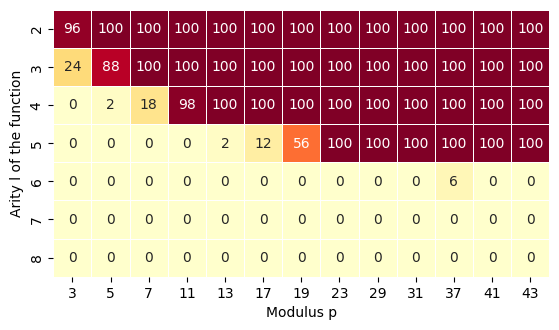
\includegraphics[]{img/p_encodings/heatmap_success.png}
    \caption{Rate of success of the algorithm for 100 random Boolean functions for different values of $\ell$ and $p$.}
    \label{fig:heatmap_success}
\end{figure}


Figure \ref{fig:lineplot_timings} shows the evolution of the time of execution of the algorithm for random Boolean functions \emph{for which no solution exists}.  It shows the explosion of the complexity for high values of
$p$, and justifies the need of a more efficient algorithm for those function (we introduce one in Section \ref{sec:graphs}).  


\TODO{Harmoniser l'algorithme suivant (commenté)}
\begin{figure}
    \centering
    \begin{minipage}{0.55\textwidth}
        \centering
        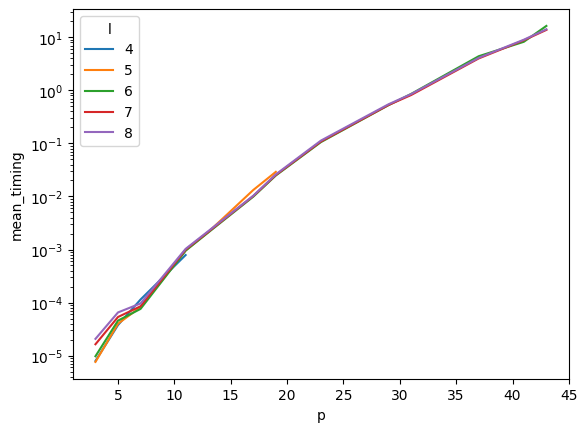
\includegraphics[width=\linewidth]{img/p_encodings/lineplot_timings.png}
        \caption{Running time of the algorithm for different values of $\ell$ and $p$ for random functions. Note that the scale is logarithmic.}        
        \label{fig:lineplot_timings}
        \end{minipage}\hspace{0.04\textwidth}
    \begin{minipage}{0.35\textwidth}
        \centering
        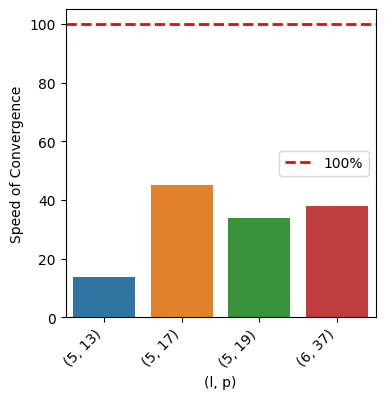
\includegraphics[width=\linewidth]{img/p_encodings/barplot.png}
        \caption{Ratio between the time to find a solution when it exists with the time to run the full algorithm when no solution exists.}
        \label{fig:barplot_ratio}
    \end{minipage}
    \caption{Some metrics about running time.}
    \label{fig:overall}
\end{figure}
Lastly, Figure \ref{fig:barplot_ratio} shows how long it takes to find a solution when one exists, relatively to the running time when no solution exist at all. It illustrates a form of "speed of convergence" and shows that it is located around $\frac{1}{3}$.



    
\subsection{An Efficient Sieving Heuristic to Find Suitable Encodings}
\label{sec:heuristic_matthieu}


Let us consider a function $f: \B^\ell \mapsto \B$ of matrix of constraints $C=(C_j^{(i)})_{\substack{1 \le i \le n_j\\1 \le j \le \ell}}$ and its associated system of linear inequalities:

$$
\left \{
\begin{array}{c}
     c_1^{(1)} \times d_1 + c_2^{(1)} \times d_2 + \dots + c_\ell^{(1)} \times d_\ell   \neq 0 \mod p\\
     c_1^{(2)} \times d_1 + c_2^{(2)} \times d_2 + \dots + c_\ell^{(2)} \times d_\ell \neq 0 \mod p\\
    \dots
\end{array}
\right .
$$


The principle is to sample random values in $\Z$ (with some large bound) and affect them to the $d_j$'s. If all the corresponding values for all the $C_i = \sum_{j=1}^{\ell} c_j^{(i)} \times d_j$ are not divisible by a value $p$, then the vector $(d_j \mod p \mid j \in \{1, \dots, \ell\})$ is a solution of the system of inequalities generated by $C$. 


To reduce the amount of samples required to find a solution, we want to avoid sampling trivially wrong sets of $d_j$'s. For example, if all the $d_j$'s are themselves divisible by $p$, then the $C_i$'s will all be divisible as well. To tackle this problem, we perform the sampling across \emph{prime numbers in $\Z$}.



%\begin{algorithm}
%    \caption{Sample a solution $\vec d$ in $\Z$ for a function $f$ and returns a possible value for $p$.}
%    \label{alg:heuristic_matthieu}
%    \begin{algorithmic}
%    \Require \\
%    $\{C_i\}_{1 \le i \le n}$ \Comment{The lines of the matrix of constraints $C$ of the function $f$ } \newline
%    $P$ \Comment{The sets of possible values for $p$ to be tested} \newline
%    $D$ \Comment{The sets of possible values in $\Z$ to assign to the $d_i$'s. All these elements are big primes}
%    \Ensure $f$ is possible to evaluate using a modulus smaller or equal than $p$.
%    \State{$\vec{d} \drawfrom D$} \Comment{Sample random prime values in $\Z$ and assign it to $\Vec{d} = (d_1, \dots, d_l)$}
%    \State{$\vec r = C \times \vec{d}$}  \Comment{$\vec r$ is the right member of the system}
%    \For {$p \in P$}
%        \If{$0 \in [\Vec{r}]_p$}          \Comment{If $p$ divides one of the coordinates of $\vec r$}
%            \State{$P \gets P \setminus \{p\}$} \Comment{This value of $p$ is incorrect}
%        \EndIf
%    \EndFor
%    \If{$\mid P \mid > 0$}
%        \State{\Return{$\min(P)$}} \Comment{Returns the smallest possible value for $p$, if any.}
%    \EndIf   
%    \end{algorithmic}
%\end{algorithm}


Running this algorithm several times and keeping the smallest returned value for $p$, one gets an upper bound on the minimum $p$ required to evaluate a function with our framework. Note that, on the contrary of the deterministic search algorithm, this heuristic does not require a prime $p$.


\paragraph{Example:} Let us consider the s-box of the block cipher ASCON. We study this s-box in more details and provide an exact optimized solution for its homomorphic evaluation in Section \ref{sec:ascon}. Here, we apply Algorithm \ref{alg:heuristic_matthieu} on the five functions generating the five output bits and monitor the results until we gather $N=10000$ non-zero possible values for $p$.


The figure \ref{fig:ascon_0_p_frequencies} shows the repartition of the returned values of $p$ by the algorithm during these $N$ runs on the first subfunction. The optimal value of $p$ found by the deterministic approach of Section \ref{sec:search_algorithm} is $17$ so the upper bound $19$ is pretty close, despite being rarely found by the algorithm. Also, the figure \ref{fig:ascon_0_count_iter} shows $21$ (the second best solution found by the sieving) is almost instantly found by the algorithm.


\begin{figure}
  \begin{minipage}{0.48\linewidth}
    \    \centering
    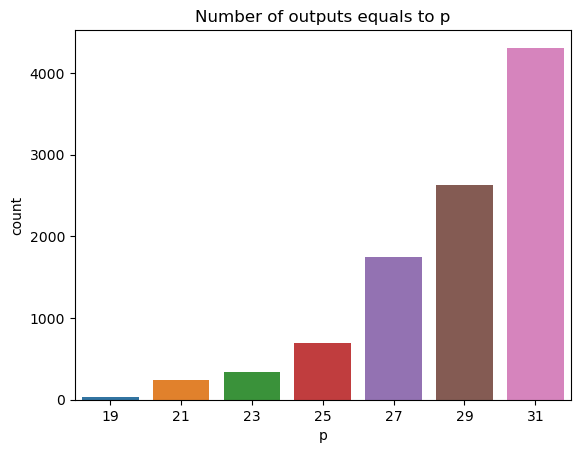
\includegraphics[width=\linewidth]{img/p_encodings/heuristic_ascon_0_p_frequencies.png}
    \caption{The outputs of $10000$ runs of the Algorithm \ref{alg:heuristic_matthieu} for the first subfunction of the Ascon s-box}
    \label{fig:ascon_0_p_frequencies}
  \end{minipage} \hfill
  \begin{minipage}{0.48\linewidth}
    \centering
    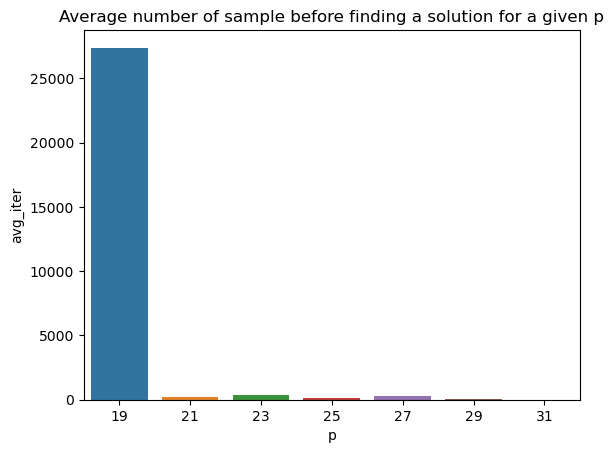
\includegraphics[width=\linewidth]{img/p_encodings/heuristric_ascon_0_count_iter.png}
    \caption{Number of iterations required to get a solution for a given value of $p$}
    \label{fig:ascon_0_count_iter}
  \end{minipage}
\end{figure}


In the process of finding the smallest $p$ possible and a correct vector of $p$-encoding to evaluate a function $f$, this heuristic is really efficient to get a tight upper bound on the value of $p$.


%\section{Scaling our Approach to any Boolean Circuit}
\label{sec:p_encodings_graphs}

Our framework optimizes the homomorphic evaluation of single Boolean functions but suffers the following limitations:

\begin{enumerate}
    \item For a Boolean function with a high number of inputs, the search algorithm may be very time-consuming.
    \item Some functions simply do not have any solution for acceptable values for $p$ ($p < 32$ for example) and thus are not efficiently evaluable in a single PBS.\footnote{The PBS can be evaluated for larger values of $p$ but it quickly becomes inefficient as $p$ grows.}
\end{enumerate}


As a consequence, we need a solution to extend our framework to these cases. In this section, we propose a strategy to leverage the circuit representation of a ``tough'' function $f$ to find a strategy of homomorphic evaluation with as few bootstrappings as possible.


\subsection{Graph of Subcircuits}
\label{sec:graph_definition}

Let $f: \B^\ell \longrightarrow \B$ be a Boolean function, and let $\mathcal{F}$ be a Boolean circuit representing $f$ (some preliminaries about Boolean circuits can be found in Section \ref{sec:p_encodings_preliminaries_boolean}). Let us describe the layout of the circuit $\mathcal{F}$. It has $\ell$ input wires, denoted by $\{y_j\}_{1 \le j \le \ell}$, and the output wire is denoted by $z$. The intermediary wires are denoted by $\{t_j\}_{1 \le j \le \theta}$. The Boolean operation gates are of fan-out 1. 


Our goal is to split the circuit into a directed acyclic graph $\mathcal{G}$, whose vertexes are subcircuits $\{\mathcal{F}_1, \dots, \mathcal{F}_k\}$ and whose edges connect the outputs of a subcircuit with the input of another. Each subcircuit $\mathcal{F}_i$ represents a subfunction $f_i: \B^{l_i} \mapsto \B$ that is evaluable with a gadget with our framework. 

We use the same notations to refer to the elements of a subcircuit $\mathcal{F}_i$ and we index them with $i$. The output of $\mathcal{F}_i$ is denoted by $z^{(i)}$ and its inputs by $\{y_j^{(i)}\}_{1 \le j \le \ell}$ and so on. 


The graph is valid for $f$ with respect to modulus $p$ if the following properties are satisfied:
\begin{itemize}
    \item Each subcircuit $\mathcal{F}_i$ has only one output $z^{(i)}$.
    \item For a subcircuit $\mathcal{F}_i$, all its inputs are either inputs of the whole circuit or outputs of other subcircuits of the graph. We can write this property as:
    $$
    \{y_j^{(i)}\}_{1 \le j \le l_i} \subset \left ( \{y_j\}_{1 \le j \le \ell} \cup \{z^{(j)}\}_{1 \le j < i} \right )
    $$
    Thus, the indexing of the $\mathcal{F}_i$'s respects the topological order of the graph, i.e. no gates of $\mathcal{F}_i$ has a child in any of the $\mathcal{F}_j$, with $j < i$.
    \item All the Boolean functions $f_i$ represented by the subcircuits $\mathcal{F}_i$ are evaluable in a single bootstrapping with modulus $p$ with our proposed method. 
    \item The last subcircuit $\mathcal{F}_c$ of the graph has $z$ (the output of the main circuit) for output: $z^{(c)} = z$.
\end{itemize}

\begin{figure}
    \centering
    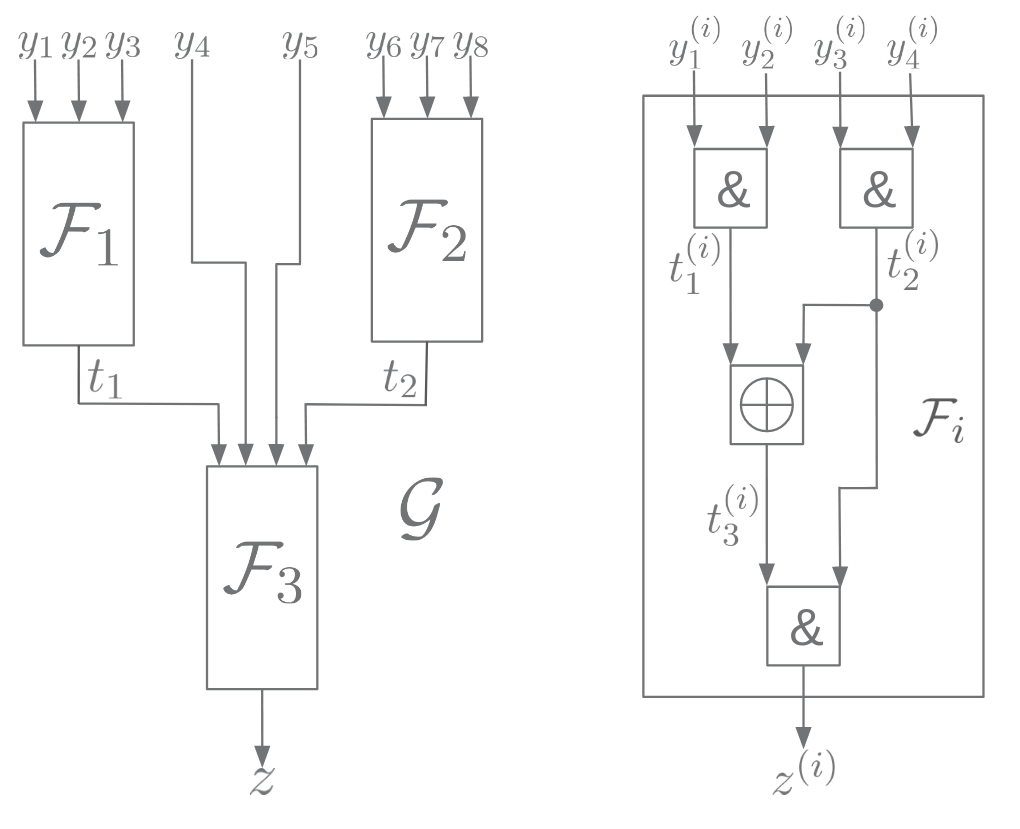
\includegraphics[width=0.75\textwidth]{img/to_harmonize/graphs.png}
    \caption{Example of graph of subcircuits (on left) and of a valid subcircuit (on right). Each subcircuit $\mathcal{F}_i$ is evaluated homomorphically with a gadget $\Gamma_i$.}
    \label{fig:enter-label}
\end{figure}




To homomorphically evaluate the function $f$, we evaluate each subcircuits with one bootstrapping for each of them and get the final result. In order to reduce the cost of evaluation for a given $p$, the goal is hence to find the \emph{smallest} valid graph possible in terms of number of subcircuits. Taking a greater value of $p$ produces a different graph that may be smaller (as subcircuits might be larger), but the timings of bootstrapping in this graph might on the other hand be greater. One can therefore run the search for different values of $p$ and keep the most efficient setup among the possible graphs. %Additionally, for some values of $p$, such a graph may not exist.

\subsection{Heuristics to Find a Small Graph}
\label{sec:heuristics_graph}

Finding such a graph can be done by exhaustively evaluating all the possible subcircuits with our method introduced in Section \ref{sec:p_encodings_search}, and then find the more efficient one. However it is not really practical to evaluate \emph{all} the possible subcircuits, so we develop some heuristics to reduce the search space. Let us start by defining a few bounds on the considered subcircuits, we will leave the other ones apart in our algorithm:

\begin{itemize}
    \item The subcircuits have at most $B$ inputs ($\forall i, l^{(i)} < B$). The purpose of this bound is to limit the running time of Algorithm \ref{alg:add_element}. In practice, for our experiments, we took $B = 10$.
    \item The subcircuits are evaluable with one single bootstrapping with a maximum value $p_{max}$. This value ensures a bootstrapping with a reasonable timing. If the search algorithm fails for $p_{max}$, the subcircuit is dropped without trying to extend $p$. In our experiment, we took $p_{max}=31$.
\end{itemize}


In order to decompose our Boolean circuit into a graph satisfying the above property for a modulus $p$, we would want to exhaustively search all the subcircuits of $\mathcal{F}$ compliant with the bounds we introduced earlier. However, all subcircuits are not equally worth to evaluate. In particular a wire incoming a copy gate is particularly worth evaluating because is costs one bootstrapping but produce several inputs for the next subcircuits. 

We gather wires that precede a copy gate in the set $\mathcal{Z}$. We add to this set the global output $z$. We also gather the input wires of the global circuit $\mathcal{F}$ in the set $\mathcal{Y}$. We define the notion of \textit{atomic subcircuit} that is a valid subcircuit whose all inputs belong to $\mathcal{Y} \cup \mathcal{Z}$ and whose output belongs to $\mathcal{Z}$. Note that the merge of two atomic subcircuits that respect the global circuit wiring is also an atomic subcircuit.

\medskip

Our heuristic works as follows:

\begin{enumerate}
    \item For each of these outputs $z_i \in \mathcal{Z}$, we exhaustively construct a set $\widehat{\mathcal{F}_{z_{i}}}$ that gathers all the atomic subcircuits whose output is $z_i$.
    We then filter out the subcircuits of $\widehat{\mathcal{F}_{z_{i}}}$ that do not comply with the bounds introduced at the beginning of the section or that are not evaluable with a gadget with the input modulus $p$ (we use Algorithm \ref{alg:add_element} to decide that).
    \medskip
    \item Now we want to construct the smallest valid graph evaluating $\mathcal{F}$ using subcircuits from the $\widehat{\mathcal{F}_{z_{i}}}$'s. While finding the smallest graph is hard, constructing any valid graph is easy. As a consequence, our strategy to find a small graph is to randomly create a lot of valid graphs and to take the smallest one. The procedure to create a valid graph is the following: we start from the output $z$ and we randomly draw a subcircuit $\mathcal{F}_z$ from $\widehat{\mathcal{F}_z}$. The inputs of $\mathcal{F}_z$ can be sorted into two categories: the ones belonging to $\mathcal{Y}$ and the ones belonging to $\mathcal{Z}$. For each one of these latter wires $w \in \mathcal{Z}$, we repeat the procedure, i.e. we draw a subcircuit $\mathcal{F}_w$ from $\widehat{\mathcal{F}_w}$, and so on. When we have reached all the input wires of $\mathcal{F}$, we get a valid graph $\mathcal{G}$ . This second step is run a large amount of times (the number of trials is a parameter of the method), and the smallest graph, i.e. the one with the fewest subcircuits, is returned.
\end{enumerate}

We carried on this method on the s-box of AES in Section \ref{sec:p_encodings_aes}.

\subsection{Parallelization of the Execution of the Graph}
\label{sec:parallelization}

Once we have our graph $\mathcal{G}$, we can identify its $n_\mathcal{L}$ \emph{layers}. Formally, they are defined as:

\begin{definition}
    A layer $\mathcal{L}$ of a graph $\mathcal{G}$ is a set of subcircuit $\{\mathcal {F}_\alpha, \dots, \mathcal{F}_\omega\}$ of $\mathcal{G}$ that verifies: $\forall \mathcal{F}_i, \mathcal{F}_j \in \mathcal{L}, \mathcal{F}_i \text{ is not an ancestor node of } \mathcal{F}_j.$    
\end{definition}

By construction, all the subcircuits belonging to the same layer can be evaluated in parallel. This reduces the number of bootstrapping steps from $k$ (the number of subcircuits in the graph $\mathcal{G}$) to $n_\mathcal{L}$ (the number of layers). Our graph-finding heuristic can be tweaked to select the graph with minimum number of layers instead of minimum number of subcircuits to optimize parallelization.

%\section{Adaptation of TFHE and the \texttt{tfhe-rs} Library}
\label{sec:TFHE_adaptation}

From a high level point of view, our technique can be seen as adding an additional layer of abstraction on top of TFHE. However things are not that simple: picking odd values for $p$ leads to some changes in the inner working of the programmable bootstrapping (PBS), and the choice of parameters is also affected by this change. Moreover, we implemented our framework by forking the \texttt{tfhe-rs} library~\cite{tfhe-rs} written in Rust. The following section covers the adaptation of the PBS and the choice of new parameters. The adaptation of the library is treated in Section \ref{sec:library}.

\subsection{Dealing with the Negacyclicity Problem for an Odd $p$}
\label{sec:solving_negacyclicity}

In the following, we explain the negacyclicity problem and how we propose to solve it. To do so, we need to dig into the details of the \texttt{BlindRotate} step of the PBS, that we have introduced in Section \ref{sec:bootstrapping}.

Let $v(X)$ be a polynomial of the ring $\Z_{q, N}[X]/(X^N+1)$, denoted by $v(X) = \sum_{k=0}^{N-1} v_k X^k$. Observe that a multiplication by $X$  in this ring ``rotates'' the coefficients of the polynomial: \[X \cdot v(X) = - v_{N - 1} + v_0 \cdot X \dots + v_{N - 2} X^{N - 1}~.\]

In TFHE, the polynomial multiplication in the blind rotation is actually done by $X^{-\Tilde{\mu}}$, with $\Tilde{\mu} = \rounding{\frac{\mu \cdot 2N}{q}}$, which lives in $\{0, \dots, 2N - 1\}$. This leads to two problems:

\begin{itemize}
    \item A coefficient $v_j$ can be brought in first place by two differents rotations: the one induced by the polynomial multiplication by $X^{\modulo{-j}{2N}}$ and the one by $X^{[-j + N]_{2N}}$.
    \item Each time a coefficient goes last to first, it gets negated (because $X^N = -1$ in the ring). So actually, the multiplication by $X^{[-j]_{2N}}$ yields correctly $v_j$, but the one by $X^{[-j + N]_{2N}}$ yields $-v_j$.
\end{itemize}


However, these problems can be circumvented for even and odd values of $p$. Recall that $\mu = m + e \in \Z_q$, with $e$ sampled from a small centered Gaussian. The use of a small error makes that $\mu$ does not take all the values of $\Z_q$ with the same probability: in particular, the densest parts in terms of probability over $\Z_q$ are the one close to the ``unscrambled'' values of $m$, namely $\left \{ \rounding{\frac {k q}{p}} \mid k \in \Z_p \right \}$. We illustrate this distribution on Figure \ref{fig:density_of_phase}. We call these sections of the torus the \emph{dense spots}.


\begin{figure}
    \begin{subfigure}{0.49\linewidth}
        \centering
        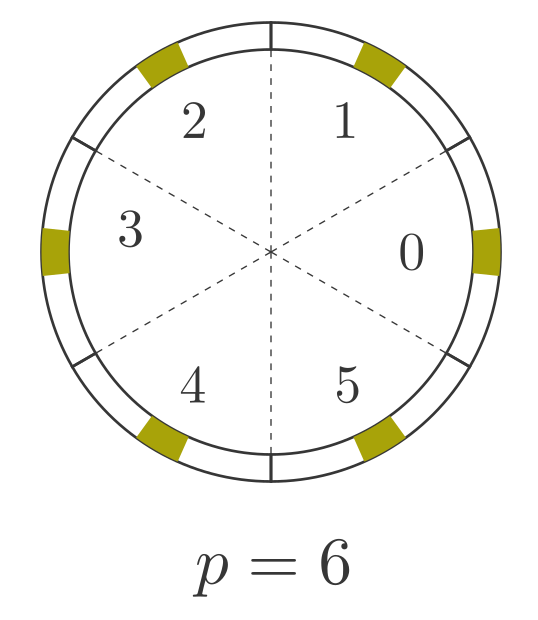
\includegraphics[width=0.5\linewidth]{img/to_harmonize/busy_sectors_2.png}
    \end{subfigure}\hspace{1em}% Adjust the margin width as needed
    \begin{subfigure}{0.49\linewidth}% Specify the width here
        \centering
        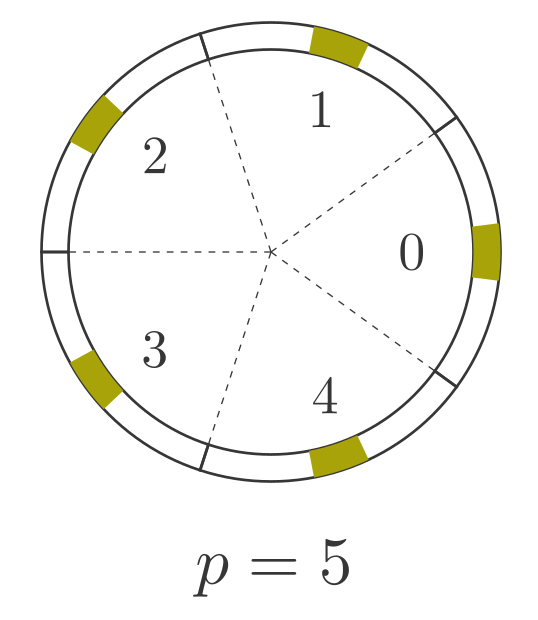
\includegraphics[width=0.5\linewidth]{img/to_harmonize/busy_sectors.png}
    \end{subfigure}
    \caption{Distribution of the values of $\mu$ across $\Z_{q}$ for $p = 6$ and $p = 5$: the colored parts show the dense spots where the value has a high probability to lie in. The width of these sectors depends on $\sigma$ (the standard deviation of the error distribution $\chi$ of TFHE). Note that this repartition looks the same for $\Tilde{\mu}$ in $\Z_{2N}$.}    
    \label{fig:density_of_phase}
\end{figure}


When we transpose these dense spots into $\Z_{2N}$, they become the sectors close to $\left \{ \rounding{\frac{k \cdot 2N}{p}} \mid k \in \Z_p \right \}$. Let us note that the noises in $\Z_q$ and $\Z_{2N}$ are fundamentally different: the former is the one added at encryption that may have grew during the homomorphic computations, and the latter is called ``drift'' and is caused by the accumulation of the rounding errors on each coefficient of the ciphertext during the modulus switching (but this difference in nature does not impact our purpose). 
Let $k \in \Z_p$, the multiplication $X^{- \frac{k \cdot 2N}{p}} \cdot v(X)$ yields the same degree-zero coefficient as the multiplication  $X^{\modulo{- \frac{k \cdot 2N}{p} + N}{2N}} \cdot v(X)$, up to the minus sign. For the sake of clarity, we write the exponent of the latter in a slightly different manner: 
\[\modulo{
    \frac{
        -k \cdot 2N
        }
    {
        p
    }
    + N
}{2N} = 
\modulo{
    \frac{
    (-k + \frac p 2 ) \cdot 2N
    }
    {p}
}
{2N}\]


This is where the parity of $p$ plays a part: if $p$ is even, then $\modulo{
    \frac{
    (-k + \frac p 2 ) \cdot 2N
    }
    {p}
}
{2N}$ is a dense spot as well. So, the rotations by these two values will happen with high probability and they will both yield the same coefficient $v_{\frac{k \cdot 2N}{p}}$ (up to the minus sign for one of them). Thus, when evaluating a function $f$ with a PBS, the calls $f(k)$ and $f(k + \frac p 2)$ will produce the same output (one again, up to the minus sign), which is a collision constraining the definition of $f$. On the other hand, let us consider an odd value for $p$. Then, $\modulo{
    \frac{
    (-k + \frac p 2 ) \cdot 2N
    }
    {p}
}{2N}$ is no longer a dense spot, as it lies exactly halfway between the two dense spots $\modulo{
    \frac{
    (-k + \frac {p-1} {2} ) \cdot 2N
    }
    {p}
}{2N}$ and $\modulo{
    \frac{
    (-k + \frac {p+1} {2} ) \cdot 2N
    }
    {p}
}{2N}$. As a consequence, collision never occurs. Figure \ref{fig:torus_p_even_vs_odd} illustrates this phenomenon.


\begin{figure}
  \begin{subfigure}{0.49\linewidth}
    \    \centering
    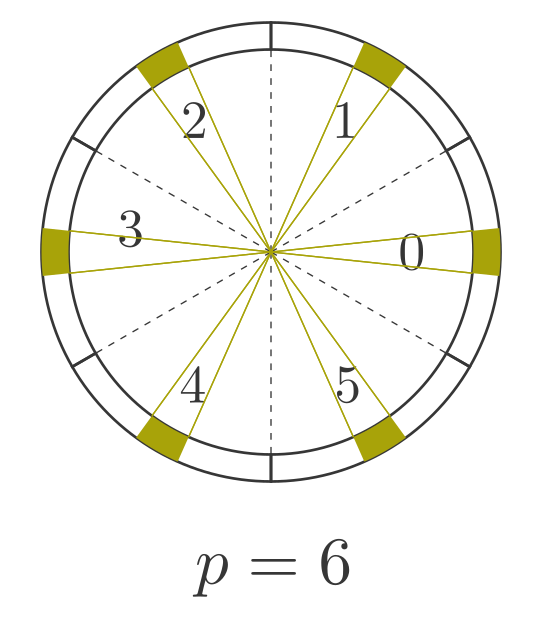
\includegraphics[width=0.5\linewidth]{img/to_harmonize/torus_p_even.png}
    \caption{With $p$ even, the dense spots of each half of the torus are aligned.}
    \label{fig:torus_p_even}
  \end{subfigure}\hspace{1em}% Adjust the margin width as needed
  \begin{subfigure}{0.49\linewidth}
    \centering
    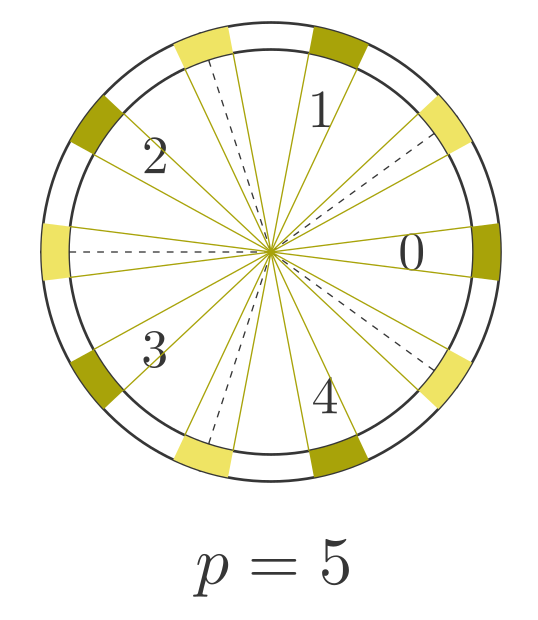
\includegraphics[width=0.5\linewidth]{img/to_harmonize/torus_p_odd.png}
    \caption{With $p$ odd, the dense spots face empty spots, close to the bounds of the $p$-sectors.}
  \end{subfigure}
  \caption{}
  \label{fig:torus_p_even_vs_odd}
\end{figure}



That is why we select only odd values for $p$ in our framework. 


We will see in Section \ref{sec:parametrization} how this change impacts the parametrization of the scheme.

\TODO{Ecrire que ça ne chanre rien au paramétrage, avec une référence sur la bonne section}






\paragraph{Exception for $p=2$:} We just said that only odd values can be selected for $p$ in our framework, however $p$-encodings with even values of $p$ exist as well: nonetheless they need to achieve the relaxed negacyclicity property introduced in Definition \ref{def:encoding}. This restriction makes them basically useless, as using only odd $p$-encodings is sufficient to evaluate all possible Boolean functions without having to bother with the negacyclicity property. However, the case $p=2$ is an exception: the valid $2$-encodings are automatically negacyclic and allow to evaluate the \texttt{XOR} operation by simply performing an homomorphic sum (so without bootstrapping). So it might be efficient to switch between $2$-encodings for \texttt{XOR} operations and $p$-encodings (with odd $p$) for non-linear Boolean functions. We make use of this strategy in our implementation of the Keccak permutation in Section \ref{sec:keccak} and for the AES in Section \ref{sec:aes}.



\subsection{Construction of the Accumulator for an Odd $p$}
\label{sec:accumulator}


The accumulator is the polynomial $v(X)$ used in the \texttt{BlindRotate} step of the PBS. In the Section \ref{sec:solving_negacyclicity}, we showed how the values are spread over the torus after bootstrapping. To actually make that works, we need to explicitly characterize this polynomial. In the following presentation, we neglect roundings to keep notations light (as if $p$ would divide $N$), or, equivalently, the division operator is assumed to include rounding.

\begin{definition}
    If $p$ is an odd modulus, and $f: \Z_p \mapsto \Z_{p'}$ a function, then the accumulator $v(X) \in \Z_{N, q}[X]/(X^N+1)$ has the form:\[v(X) = X^{- \frac {N} {2p}} \cdot \sum_{j=0}^{N/p - 1} X^j  \cdot \left ( \sum_{i=0}^{\frac{p-1}{2}} f(i) X^{i \frac{2N}{p}} + \sum_{i=0}^{\frac{p-1}{2} - 1} -f \left (i + \frac{p+1}{2} \right ) X^{i \frac{2N}{p} + \frac N p} \right )\]
\end{definition}


Let us explain the structure of this accumulator. The polynomial has degree $N$ and is made of $p$ distinct windows of width $\frac{N}{p}$. Each of these windows has constant coefficient value $f(k)$, for $k \in \{0, \dots, p-1\}$.
For $0 \le \alpha \le \frac{p-1}{2}$, the range of degrees whose coefficients are $f(\alpha)$ is $\left [ \alpha \frac{2N}{p} - \frac{N}{2p}~;~ \alpha \frac{2N}{p} + \frac{N}{2p} \right ]$. Now, for $\frac{p+1}{2} \le \beta \le p-1$, we can write $\beta = \alpha + \frac{p+1}{2}$, with $0 \le \alpha < \frac{p-1}{2}$. This time, the range of spanned degrees is $\left [ \alpha \frac{2N}{p} + \frac{N}{2p} ~;~ (\alpha + 1) \frac{2N}{p} - \frac{N}{2p} \right ]$. Thus, the values $k \in \{0, \dots, p-1\}$ spans the entire space $[0; N)$ without overlap. The values over $\frac{p+1}{2}$ gets negated by the negacyclicity, so the underlying coefficient is also negated to compensate this effect. We illustrate this construction on Figure \ref{fig:accumulator}.

\begin{figure}
    \centering
    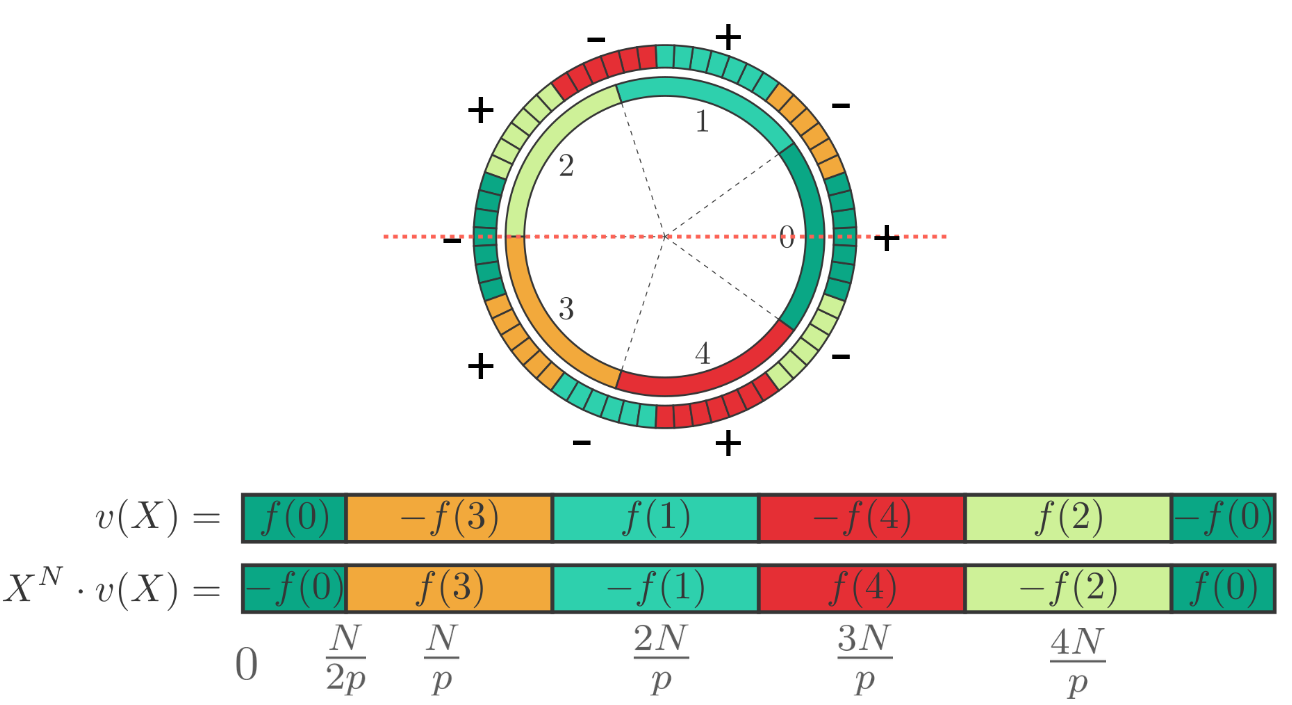
\includegraphics[width=\textwidth]{images/accumulator.png}
    \caption{Illustration of the construction of the accumulator. On top is the ring $\Z_{2N}$ splitted in windows. Below is a representation of the polynomial $v$, with its version once rotated by a multiplication by $X^N$. On the figure, $p$ = 5.}
    \label{fig:accumulator}
\end{figure}



\subsection{Crafting of Parameters}
\label{sec:parametrization}
The instances of the TFHE scheme are defined by a set of parameters. These parameters should simultaneously ensure the security of the scheme and the correctness of the homomorphic computations. They also determine the time of execution of one PBS. Here we define a framework to dimension the parameters required to optimally execute a given gadget.

Finding an optimal set of parameters for a given application is a hard problem and has been studied in particular in \cite{zama_parameters_optimization}. The parameters need to ensure three properties: security, correctness and efficiency. 

Let us start by an overview of the different parameters at play in an instance of the TFHE bootstrapping:

\begin{itemize}
    \item $n$: the dimension of the \LWE samples. Namely, the TLWE ciphertexts are vectors of length $n + 1$.
    \item $q$: the modulus of the ring the encrypted values live on. In \texttt{tfhe-rs} those values are stored on \texttt{u32} values, making $q = 2^{32}$. We treat this as an immutable platform-dependent value.
    \item $\sigma$: the standard deviation of the Gaussian distribution of error in \LWE samples.
    \item $k$: the dimension of the \GLWE samples. If $k=1$, we talk about \RLWE samples.
    \item $\sigma'$: the standard deviation of the Gaussian distribution of error in \GLWE samples.
    \item A few more parameters dimensioning some inner algorithms of the bootstrapping. A detailed description and an analysis of their impact on performances and noise level can be found in \cite{zama_parameters_optimization}. In this work, they are denoted as \emph{micro-parameters}.
\end{itemize}

In \cite{zama_parameters_optimization}, authors elaborate a strategy where they define an \textit{atomic pattern} of FHE operators, that is to say a subgraph of FHE operators in which the noise of the output is independent from the one in the inputs. Then, they develop an optimization framework to derive the best set of parameters for a given atomic pattern.

In particular, the first atomic pattern they study, that they denote by $\mathcal{A}^{(CJP21)}$, is a subgraph composed of a linear combination of ciphertexts with clear constants, then a \texttt{Keyswitch} and then a \texttt{BlindRotate} followed by a \texttt{SampleExtract} (\texttt{ModulusSwitch} is seen as a part of \texttt{BlindRotate}). Note that in Section \ref{sec:bootstrapping} we introduced the bootstrapping of TFHE by putting the \texttt{BlindRotate} before the \texttt{Keyswitch}, but the other way around is also doable. To dimension the parameters of TFHE to evaluate such an atomic pattern, their framework takes as input the 2-norm of the vector of constants of the linear combination (denoted by $\nu$) and a noise bound $t$ on the standard deviation of the distribution of error in a ciphertext that ensures a correct decryption with a good probability $(1-\epsilon$). We elaborate further on how this bound is constructed below in this section.

If we look closely, the evaluation of a gadget we introduced in Definition \ref{def:gadget} can be seen as a $\mathcal{A}^{(CJP21)}$ with a few differences. Thus, we slightly modified the tool \texttt{concrete-optimizer} \cite{concrete-optimizer}, that allows to generate parameters for different types of atomic patterns, to support our gadget as a new atomic pattern. Let us dive into the differences between a gadget and a $\mathcal{A}^{(CJP21)}$:

\paragraph{Support of odd values for $p$:} Using an odd value for $p$ changes the bootstrapping procedure, and in particular the definition of the accumulator for the \texttt{BlindRotate} (as explained in Section \ref{sec:accumulator}). With our construction, the windows in the polynomial are half the size of the ones for an even $p$, which impacts the noise bound $t$. 
As this bound depends of the failure probability $\alpha$ that the user is ready to tolerate, we shall denote it $t_\alpha$ hereafter, which satisfies: $t_\alpha = \frac{\Delta}{2z^*(1-\sqrt[N]{1-\alpha})}$
where $z^*$ is the \emph{standard score} and $\Delta$ is the scaling factor (see~\cite{zama_parameters_optimization} for more explanations). The impact of our adaptation on this formula is solely with respect to the scaling factor. In the context of an $\mathcal{A}^{(CJP21)}$, we have $\Delta = \frac{q}{2^\pi p}$ with $\pi$ the number of MSB for padding. As explained in Section \ref{sec:solving_negacyclicity}, we do not need any padding mechanism anymore, so the $2^\pi$ vanishes. However, the length of a window is divided by $2$, and $p$ does not divide $q$ anymore so we need to add a rounding. We finally get $\Delta = \rounding{\frac{q}{2p}}$.


\paragraph{Link between input encodings and $\nu$:} In a scenario where only one gadget has to be evaluated, its inputs are freshly encrypted ciphertexts. Then, there is no need to perform any encoding switching before evaluating the gadget, and so we are in the context of a $\mathcal{A}^{(CJP21)}$ with $\nu = 1$. However, if we are in a context of a \textit{graph} of gadgets like in Section \ref{sec:graphs}, the output of a gadget can be used as input of subsequent gadgets under different encodings. In this case, some encoding switchings are necessary. If these encoding switching are made using a mutiplication by a constant (Property \ref{prop:mult_constant}), we are still in the context of a $\mathcal{A}^{CJP21}$ but with $\nu \ne 1$. 
To formalize that, we first recall that Algorithm \ref{alg:add_element} produces gadgets of the form $\Gamma = \left (\vec{\Encoding_{in}}, \Encoding_{out}, p_{in}, p_{out}, f \right )$, with $\Encoding_{in}^{(i)} = \EncDefOne{d_i}$. Thus, if we fix that all gadget output ciphertexts are encoded under $\Encoding_{out} = \EncDefOne{1}$, then the encoding switchings needed before an evaluation of $\Gamma$ corresponds to a linear combination of the inputs with the vector $\vec d = (d_i \mid i \in [1, \ell])$, so we fall back on a $\mathcal{A}^{(CJP21)}$ with $\nu = \customnorm{\vec d}$.


We implemented these changes in \texttt{concrete-optimizer} and uses it to generate sets of parameters for our implementations detailed in Section \ref{sec:implementations}.

\subsection{Concrete Implementations of $p$-Encodings and Homomorphic Functions in \texttt{tfhe-rs}}
\label{sec:library}


To implement our framework, we relied on the $\texttt{tfhe-rs}$ library~\cite{tfhe-rs}. Here is a list of the major changes we applied to the code:

\paragraph{Addition of the notion of $p$-encoding: } An encoding $\Encoding$ is simply implemented with a structure \texttt{Encoding} storing two \texttt{HashSets} and the modulus $p$. The \texttt{HashSets} represent both sets $\Encoding(0)$ and $\Encoding(1)$. When creating an \texttt{Encoding}, the code checks whether the two underlying sets are disjoint or not. Moreover, the operation of encryption and decryption are modified as well. The signatures change from:\[\texttt{encrypt(Boolean, ClientKey) -> Ciphertext}\] to: \[\texttt{encrypt(Boolean, ClientKey, Encoding) -> Ciphertext}\] (same for \texttt{decrypt}). The functions also perform the mapping $\B \mapsto \Z_p$ before encryption and the other way around after decryption.


\paragraph{Support of odd moduli: } The native \texttt{tfhe-rs} only support power-of-two-moduli $p$. We extended the library to handle odd values for $p$. This required modifying the encryption and decryption algorithm, and to compute the sets of parameters with the method of Section \ref{sec:parametrization}.


\paragraph{Definition of the new structure $\texttt{Gadget}$: } According to the evaluation strategy we introduced in Section \ref{sec:new_strategy}, we wrote a new structure $\texttt{Gadget}$, associated to a Boolean function $f: \B^\ell \mapsto \B$, carrying:
\begin{itemize}
    \item A list of the \texttt{Encoding} objects for the inputs: $\Encoding_{in} = (\Encoding_1, \dots, \Encoding_l)$, with the input modulus $p_{in}$ they encoded on.
    \item The output \texttt{Encoding} object $\Encoding_{out}$, with the output modulus $p_{out}$ it is encoded on.
    \item The clear function $f$.
\end{itemize}
When such a structure is constructed, it self-checks whether $f(\Encoding_{in})$ is valid. Then, when provided $\ell$ $\texttt{Ciphertexts}$ objects encoded under their respective $p$-encoding, it executes the homomorphic sum and the PBS and outputs the results encoded under $\Encoding_{out}$. Some utilitary functions performing encoding-switching are also available, allowing the chaining of several $\texttt{Gadget}$.


\paragraph{Implementation of the accumulator: } The procedure of bootstrapping of \texttt{tfhe-rs} is slightly modified to support the new version of the accumulator we introduced in Section \ref{sec:accumulator}.

\paragraph{Parsing of graphs: } We implemented a Python script that produces graphs to represent more complex functions that requires several PBS, as described in Section \ref{sec:graphs}. These graphs are stored with a comprehensive file format and our Rust implementation has a module of parsing allowing to load these graphs and automatically generate the corresponding graph of \texttt{Gadget}.




%
\section{Application to Cryptographic Primitives}
\label{sec:p_encodings_implementations}


In this section, we apply our approach on some cryptographic primitives. For each primitive, we first explain the construction of the gadgets required and report the concrete performances of our implementation. We detailed all the timings of our experimentations along with the sets of parameters we used in Section \ref{sec:tables_perfs}.

For performance measurement, we implemented our framework in our fork of the library \texttt{tfhe-rs} \cite{tfhe-rs} adapted as discussed in Section \ref{sec:TFHE_adaptation} and we generated the sets of parameters thank to our version of \texttt{concrete-optimizer} \cite{concrete-optimizer}. By default, we tailored the sets of parameters to limit the probability of failure $\epsilon$ of a bootstrapping to $2^{-40}$, and a security level of $\lambda = 128$ bits. All experiments have been carried out on a laptop with a 12th Gen Intel(R) Core(TM) i5-1245U CPU with 10 cores and a frequency of 4.4 GHz, and 16 GB of RAM.


\subsection{SIMON Block Cipher}
\label{sec:simon}

SIMON is a hardware-oriented block cipher developed in \cite{simon}, which relies only on the following operations: \texttt{AND}, rotation, \texttt{XOR}. It is a classical Feistel network for which the Feistel function consists in applying basic operations on the branch, xoring the subkey and then xoring the result with the other branch as depicted in the Figure~\ref{fig:simon_cipher} (on this figure, $S^i$ denotes the left circular shift by $i$ bits.). We use one ciphertext per bit so the rotation operation is essentially free. Note that the key is considered as a plaintext, which does not change anything in the framework. In our implementation, we considered a (128-128) instance of SIMON (i.e. the whole state and the key are of size 128). 


% \begin{wrapfigure}{r}{5.5cm}
% 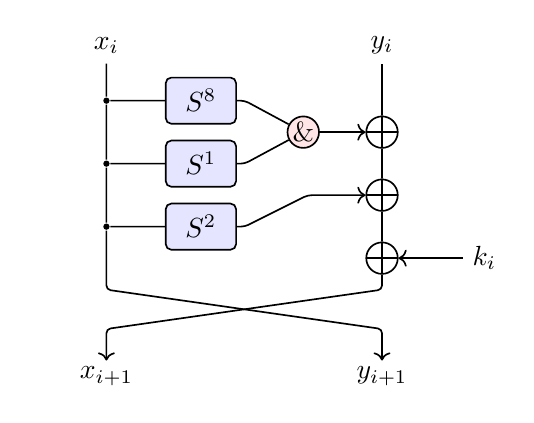
\begin{tikzpicture}
  [line width=0.6,trim left,
   shiftbox/.style = {
     draw, fill=blue!10, rounded corners=2pt,
     inner xsep=0.25cm, inner ysep=0.15cm,
   },
   wire/.style = {
     rounded corners=1.5pt
   },
   xor/.style = {
     draw, circle, inner sep=0cm, minimum size=0.4cm,
     append after command = {
       [shorten >=\pgflinewidth, shorten <=\pgflinewidth,]
       (\tikzlastnode.north) edge (\tikzlastnode.south)
       (\tikzlastnode.east) edge (\tikzlastnode.west)
     }
   },
   odot/.style = {
     draw, circle, inner sep=0cm, minimum size=0.4cm,fill=red!10
   },
   dot/.style = {
     fill, circle, inner sep=0cm, minimum size=0.08cm
   }]

  %Draw nodes
  \node at (1,6.7) (xin) {$x_i$};
  \node at (4.5,6.7) (yin) {$y_i$};
  \node[dot] at (1,6) (d1) {};
  \node[dot] at (1,5.2) (d2) {};
  \node[dot] at (1,4.4) (d3) {};
  \node[shiftbox] at (2.2,6) (S1) {$S^8$};
  \node[shiftbox] at (2.2,5.2) (S2) {$S^1$};
  \node[shiftbox] at (2.2,4.4) (S3) {$S^2$};
  \node[xor] at (4.5,5.6) (x1) {};
  \node[xor] at (4.5,4.8) (x2) {};
  \node[xor] at (4.5,4.0) (x3) {};
  \node[odot] at (3.5,5.6) (AND) {\&};
  \node at (5.8,4.0) (k) {$k_i$};
  \node at (1, 2.5) () {$x_{i+1}$};
  \node at (4.5, 2.5) () {$y_{i+1}$};

  %Draw wires
  \draw[wire] (d1) -- (S1)  (S1.east) -- +(0.1,0) -- (AND);
  \draw[wire] (d2) -- (S2)  (S2.east) -- +(0.1,0) -- (AND);
  \draw[wire,->] (AND) -- (x1);
  \draw[wire,->] (d3) -- (S3) (S3.east) -- +(0.1,0) -- ++(0.9,0.4) -- (x2);
  \draw[wire,->] (xin) -- (d1) -- (d2) -- (d3)
                  -- ++(0,-0.8) -- ++(3.5,-0.5) -- ++(0,-0.4);
  \draw[wire,->] (yin) -- (x1) -- (x2) -- (x3)
                 -- ++(0,-0.4) -- ++(-3.5,-0.5) -- ++(0,-0.4);
  \draw[wire,->] (k.west) -- (x3);
\end{tikzpicture} 
%    \caption{One Feistel round of SIMON. }   
%    \label{fig:simon_cipher}
% \end{wrapfigure}

\begin{figure}
    \centering
    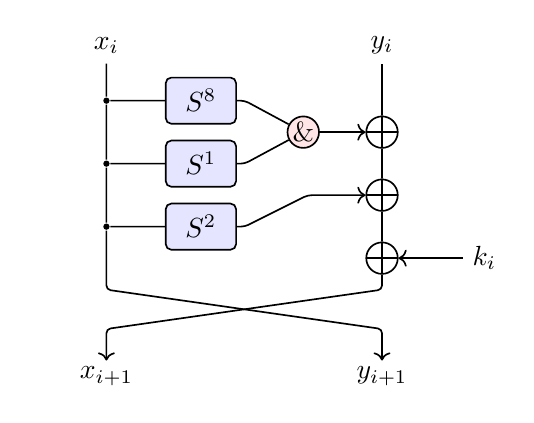
\begin{tikzpicture}
  [line width=0.6,trim left,
   shiftbox/.style = {
     draw, fill=blue!10, rounded corners=2pt,
     inner xsep=0.25cm, inner ysep=0.15cm,
   },
   wire/.style = {
     rounded corners=1.5pt
   },
   xor/.style = {
     draw, circle, inner sep=0cm, minimum size=0.4cm,
     append after command = {
       [shorten >=\pgflinewidth, shorten <=\pgflinewidth,]
       (\tikzlastnode.north) edge (\tikzlastnode.south)
       (\tikzlastnode.east) edge (\tikzlastnode.west)
     }
   },
   odot/.style = {
     draw, circle, inner sep=0cm, minimum size=0.4cm,fill=red!10
   },
   dot/.style = {
     fill, circle, inner sep=0cm, minimum size=0.08cm
   }]

  %Draw nodes
  \node at (1,6.7) (xin) {$x_i$};
  \node at (4.5,6.7) (yin) {$y_i$};
  \node[dot] at (1,6) (d1) {};
  \node[dot] at (1,5.2) (d2) {};
  \node[dot] at (1,4.4) (d3) {};
  \node[shiftbox] at (2.2,6) (S1) {$S^8$};
  \node[shiftbox] at (2.2,5.2) (S2) {$S^1$};
  \node[shiftbox] at (2.2,4.4) (S3) {$S^2$};
  \node[xor] at (4.5,5.6) (x1) {};
  \node[xor] at (4.5,4.8) (x2) {};
  \node[xor] at (4.5,4.0) (x3) {};
  \node[odot] at (3.5,5.6) (AND) {\&};
  \node at (5.8,4.0) (k) {$k_i$};
  \node at (1, 2.5) () {$x_{i+1}$};
  \node at (4.5, 2.5) () {$y_{i+1}$};

  %Draw wires
  \draw[wire] (d1) -- (S1)  (S1.east) -- +(0.1,0) -- (AND);
  \draw[wire] (d2) -- (S2)  (S2.east) -- +(0.1,0) -- (AND);
  \draw[wire,->] (AND) -- (x1);
  \draw[wire,->] (d3) -- (S3) (S3.east) -- +(0.1,0) -- ++(0.9,0.4) -- (x2);
  \draw[wire,->] (xin) -- (d1) -- (d2) -- (d3)
                  -- ++(0,-0.8) -- ++(3.5,-0.5) -- ++(0,-0.4);
  \draw[wire,->] (yin) -- (x1) -- (x2) -- (x3)
                 -- ++(0,-0.4) -- ++(-3.5,-0.5) -- ++(0,-0.4);
  \draw[wire,->] (k.west) -- (x3);
\end{tikzpicture} 
    \caption{One Feistel round of SIMON. }     
    \label{fig:simon_cipher}
\end{figure}


The Boolean function to evaluate can be defined as $$f(b_0, b_1, b_2, b_3, b_4) = b_0 \cdot b_1 \oplus b_2 \oplus b_3 \oplus b_4~.$$


Using Algorithm \ref{alg:add_element}, we found the smallest possible $p$ ($p = 9$) and the following $9$-encodings to evaluate each bit of the Feistel function with one single bootstrapping (i.e. totalling 64 PBS per round). 


\[\Encoding_0 = \Encoding_1 = \EncDefOne{1} \text{ and } \Encoding_2 = \Encoding_3 = \Encoding_4 = \EncDefOne{2} \text{ with } p = 9.\] The sum of these $p$-encodings yields the output encoding: \[\Encoding_{out} = \EncDef{\{0, 1, 4, 5, 8\}}{\{2, 3, 6, 7\}} \text{ with } p=9\] which is valid for $f$. After the PBS, all the bits of the state are encrypted under the encoding $\Encoding_0$. We formalize that with the gadget $\Gamma = \left ((\Encoding_0, \Encoding_1, \Encoding_2, \Encoding_3, \Encoding_4), \Encoding_0, 9, 9\right )$


To perform a Feistel round on a state of size $k$, the gadget $\Gamma$ is applied in parallel $k / 2$ times. Note that one bit may be used in several evaluation as $b_0$, $b_1$ and $b_2$. So we sometimes have to switch from $\Encoding_0$ to $\Encoding_1$ by a simple external multiplication by $2$, which is negligible in terms of performances.


Using our version of \texttt{concrete-optimizer} \cite{concrete-optimizer}, we crafted a set of parameters suitable for this modulus and these encodings. 
On our machine, one PBS with such parameters takes about $9.5$ ms. The theoretical timings achieved on one full block without any parallelization is $41$ seconds ($68$ rounds $\times$ $64$ bits $\times$ $9.5$ ms)  which we confirmed experimentally.


Nonetheless, this setting is intrinsically parallelizable: the 64 gadgets of each round can be performed in parallel. We implemented parallelization using the module \texttt{Rayon} of Rust, which made the total timings drop to $13$ seconds on our machine. 

Compared to \cite{DBLP:conf/fps/BendoukhaSSQS22} that implemented the same block cipher on an equivalent hardware with parallelism, our implementation is about 10 times faster. Table \ref{tab:concrete_perfs} shows the comparison. Note that in this paper, the probability of failure is not specified. As ours is pretty conservative, this is a good argument in favor of our framework.


\subsection{The Trivium Stream Cipher}
\label{sec:trivium}

Trivium \cite{ISC:DeCanniere06} is a stream cipher that uses a circular state. At each round, the bits are rotated within the state, except for three of them that are refreshed using the Boolean function of Section \ref{sec:simon}. The outer stream is generated by xoring three bits of the state each round once a ``warming-up'' phase is achieved. 


For each generated key bit, it requires performing this function three times and aggregating five \texttt{XOR} operations in the center. Our strategy is to evaluate the refreshing function three times per round with one PBS for each of them, then get the result in $\Z_2$ and chain the five \texttt{XOR} operations to get the output.
Figure \ref{fig:triviuml} illustrates the layout of the cipher.
\begin{figure}
    \centering
    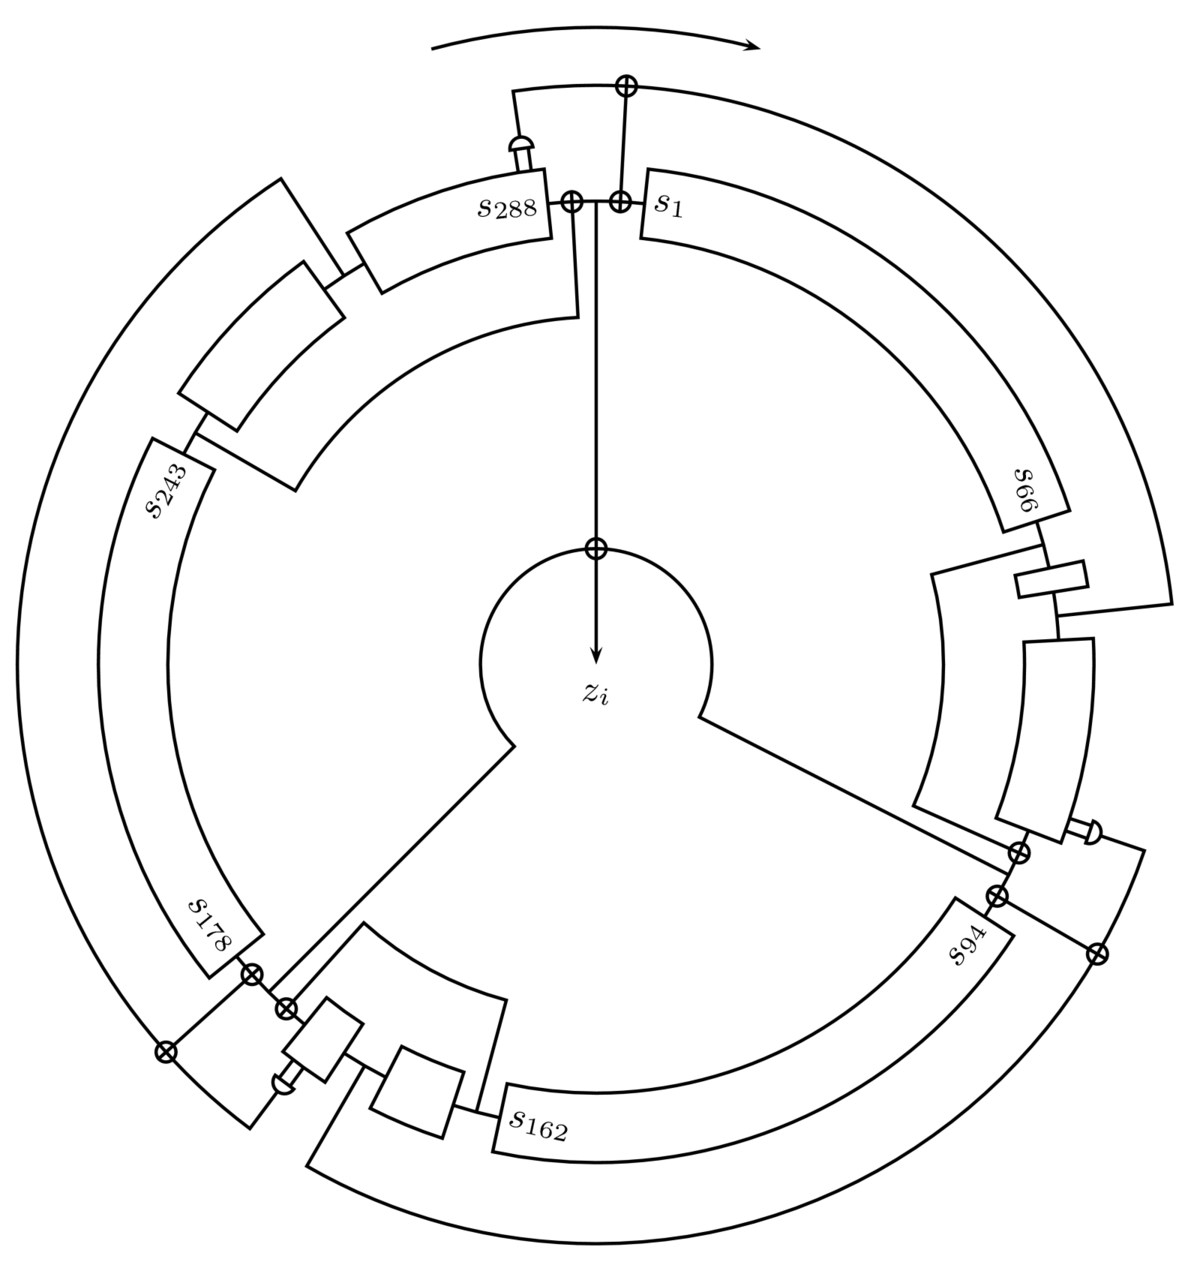
\includegraphics[width=0.5\linewidth]{img/to_harmonize/trivium.png}
    \caption{The trivium stream cipher. Figure extracted from \cite{ISC:DeCanniere06}}.
    \label{fig:triviuml}
\end{figure}


In \cite{DBLP:conf/wahc/BalenboisOS23}, the authors implement Trivium using the original \texttt{tfhe-rs} library, with 2 bits of message and 2 bits of carry for a total of 4 significative bits out of the 32 of a ciphertext component. They call this mode the \texttt{shortint} mode. The use-case they target is transciphering.

To compare our implementation with the one of \cite{DBLP:conf/wahc/BalenboisOS23}, timings are not a good metric as in their work they are provided on a massive AWS instance with a significant amount of parallelism. A better metric is to count the number of PBS and compare the parameter sets.

We reproduced the PBS operation with their parameter set on our machine and then simply estimated the timings of one round of Trivium with their approach with no parallelism. The results are summed up in Table \ref{tab:perfs_trivium}. Note that in our implementation we do not refresh the output bits with a PBS after the chain of \texttt{XOR}, because in the use-case of transciphering one more \texttt{XOR} has to be performed with the message. We take advantage of this and move the last PBS into the transciphering phase.

\begin{table}[htbp]
\centering
\caption{Comparison of timings of one round of Trivium between our work and \cite{DBLP:conf/wahc/BalenboisOS23}, with $\epsilon=2^{-40}$.}
\label{tab:perfs_trivium}
\begin{tabular}{|c|c|c|c|}
\hline
Instance & Timing PBS & Number of PBS per round & Estimated timings \\
\hline
\cite{DBLP:conf/wahc/BalenboisOS23} & 6.6 & 7 & 46.2 ms \\
\hline
Our work & 9.5 & 3 & 28.5 ms \\
\hline
\end{tabular}
\end{table}

\subsection{Keccak Permutation}
\label{sec:keccak}

Keccak is a hash function standardized by NIST under the name \emph{SHA-3} \cite{sha-3}. It is a sponge function, whose transformation is called the \emph{Keccak permutation}. It consists of five sub-functions: $\theta$, $\rho$, $\pi$, $\chi$, and $\iota$.

Let us recall that our approach encrypts each bit in one TFHE ciphertext. Let us explain the stategies of homomorphization of these sub-functions:
\begin{itemize}
    \item $\rho$ and $\pi$ simply reorder the bits within the state, so they are not impacted by the homomorphization.
    \item $\theta$ is just a serie of \texttt{XOR} operations, so it can be performed with a serie of homomorphic additions and without any PBS provided that the input ciphertexts are defined over $\Z_p$ with $p=2$.
    \item $\chi$ is the only non-linear function of the permutation, and has to be performed with a PBS. It is the transformation that applies the function defined by $$f_\chi(a, b, c) = a \oplus c \oplus b \& c$$ to get each bit of the output state.
    \item Finally, $\iota$ performs a simple \texttt{xor} with a constant, so it can be handled in a similar manner that $\theta$. The difference is that the constant is in clear this time.
\end{itemize}
The $p$-encodings we use are:
\begin{itemize}
    \item $\Encoding_{\&} = \EncDef{\{1\}}{\{2\}}$ with $p_\& = 3$  to evaluate the $\&$ operator in the alternative formula of $\chi$.
    \item $\Encoding_\oplus = \EncDefOne{1}$ with $p_\oplus = 2$ for the other operations of $\oplus$.
\end{itemize}
Our strategy of homomorphic evaluation of the Keccak permutation is as follows:
\begin{enumerate}
    \item Encrypt the input state under the encoding $\Encoding_\oplus$.
    \item Evaluate the subfuctions $\theta$, $\rho$, and $\pi$. Theses functions being purely linear, they can be performed only with sums under $\Encoding_\oplus$.
    \item Change the encoding from $\Encoding_\oplus$ to $\Encoding_\&$ with one PBS per bit of the state (Property \ref{prop:enc_switch_pbs}).
    \item Evaluate the \texttt{AND} operator of the subfunction $\chi$ with the gadget \[\Gamma_\& = \left ( (\Encoding_\&, \Encoding_\&), \Encoding_\oplus, 3, 2\right )\] associated to function $f_\& : (x, y) \mapsto x \& y$. This gadget is applied once per bit of the state.
    \item Evaluate the remaining $\oplus$ operators of $\chi$ and the $\iota$ subfunctions, then jump back Step 2. for the next loop iteration.
\end{enumerate}


Casting a ciphertext from $\Encoding_\oplus$ to $\Encoding_\&$ (Step 3) is a bit tricky because $p_\oplus = 2$ is even. Because of the negacyclicity problem, one needs $\Encoding_\&(0) = \modulo{-\Encoding_\&(1)}{p_\&}$. With $p_\& = 3$, the only candidate is the encoding $\Encoding_\&$ defined above.


As a result, each round takes two programmable bootstrappings per bit. An implementation with our tweaked version of \texttt{tfhe-rs} takes 16.5 seconds (without any parallelism) on our hardware to perform one Keccak round on a state of 1600 bits in spite of the two PBS required per round and per bit. Those timings are possible because of the small values of $p$ allowing the use of a set of  small parameters, which speeds up the computation. A full run of Keccak counting 24 rounds, we can then estimate the timings without parallelism to $6.6$ minutes. For the sake of simplicity, we use the same set of parameters for both types of PBS, avoiding the hassle of using two different server keys.


This strategy of implementation complies with the more generic one that we introduce in Section \ref{sec:ascon} and that is illustrated on Figure \ref{fig:layout_spn}. It suits very well the use-cases where linear and non-linear operations are alternating.


\subsection{Ascon}
\label{sec:ascon}


Ascon \cite{JC:DEMS21} is a lightweight block cipher algorithm that was designed to provide efficient and secure encryption and authentication for a wide range of applications, particularly in resource-constrained environments such as embedded systems and IoT devices. The name ``Ascon'' stands for ``Authenticated encryption for Small Constrained Devices''. We implemented its s-box, whose circuit is represented on Figure \ref{fig:ascon}.

\begin{figure}[h]
    \centering
    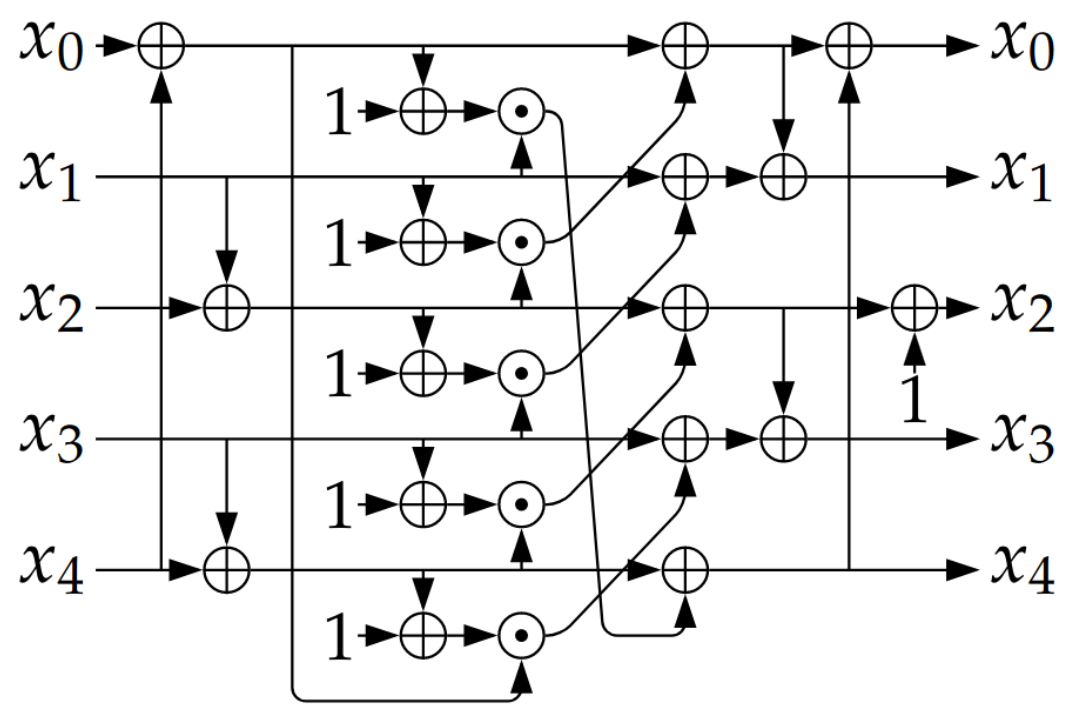
\includegraphics[width=0.5\linewidth]{img/to_harmonize/ascon.png}
    \caption{The 5-bits look-up table of ASCON. Figure extracted from \cite{JC:DEMS21}}
    \label{fig:ascon}
\end{figure}



This layout is a bit different from the others: the s-box takes five bits as input and outputs five bits. We denote $f_0, \dots, f_4$ the five functions of $\B^5 \mapsto \B$ that generate the 5 output bits $x_0, \dots, x_4$. Thus, we need to define five gadgets (one per function).

These functions, once analyzed by the algorithm, can be computed in one single bootstrapping each, but for different values of $p$ (respectively $p=17, 7, 7, 15, 11$ that are the smallest possible values). We could implement the gadgets $\Gamma_0, \dots, \Gamma_4$ (associated to $f_0, \dots, f_4$) with different values for $p_{in}$, but this would imply to introduce some encoding switchings before each round of hashing. To keep things simpler we generated only encodings with $p = 17$, making the implementation more straightforward as no encoding switching is required. For each subfunction $f_i$, five canonical $17$-encodings $(\Encoding_{i, 0}, \dots, \Encoding_{i, 4})$ of form $$\Encoding_{i, j} = \EncDefOne{d_{i,j}}$$ are computed. The results are displayed in the Table \ref{tab:encodings_ascon}. Note the zero values in some cases, they show that the variable is not used in the subfunction. 

The s-box layer is followed by a linear layer, where the bits of the states are shifted and combined with \texttt{XOR} operations. This can be trivially done with $p=2$. Finally, to prepare the next round, an encoding switching is performed to send back the ciphertexts on $17$-encodings. This is summed up in Figure \ref{fig:layout_spn}. Note that there is no encoding switching from non-linear layer to linear layer because the gadgets can directly outputs ciphertexts under $\Encoding_\oplus = \EncDefOne{1}$ with $p=2$.

\begin{figure}
    \centering
    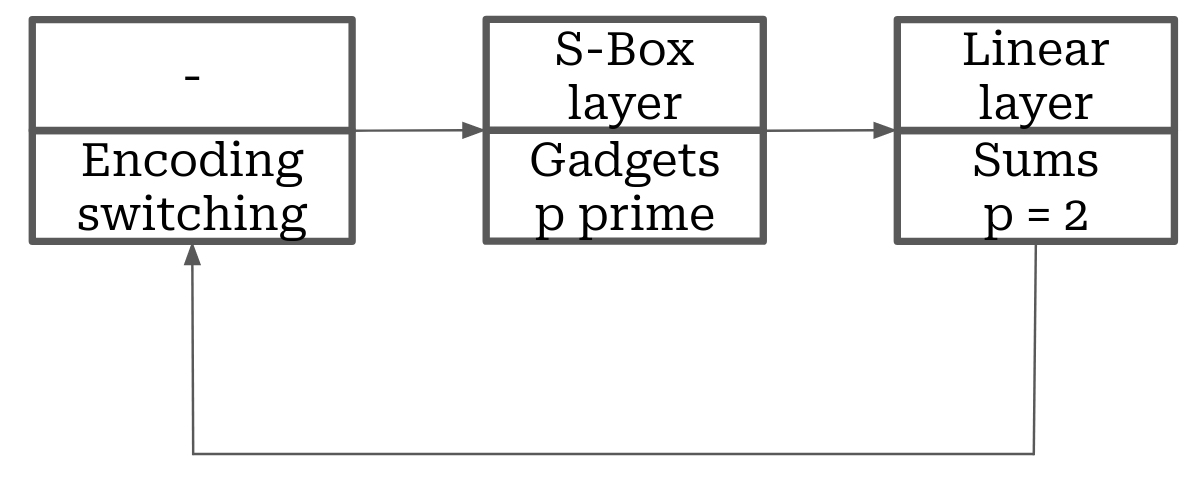
\includegraphics[width=0.5\linewidth]{img/to_harmonize/layout_spn.png}
    \caption{A common layout to evaluate cryptographic primitives. The upper part of the boxes represents what happens in the clear, while the lower part shows the encrypted operations. }
    \label{fig:layout_spn}
\end{figure}


To wrap up, we construct the five gadgets $\Gamma_i = \left ( (\Encoding_{i,0}, \dots,  \Encoding_{i, 4}), \Encoding_\oplus, 17, 2, f_i \right )$. They will carry the evaluation of the s-boxes and output ciphertexts encrypted under $\Encoding_\oplus$. Then, the linear layer is trivially evaluated with homomorphic sums. An encoding switching from $\Encoding_\oplus$ to $\Encoding_{i, j}$ allows to come back to non-linear operations.




\begin{table}[]
    \centering
    \begin{tabular}{|c|c|c|c|c|c|}
        \hline
       subfunction & $d_{i, 0}$ & $d_{i, 1}$ & $d_{i, 2}$ & $d_{i, 3}$ & $d_{i, 4}$\\
        \hline
        $f_0$  & $1$ & $2$ & $3$ & $7$ & $14$\\
        \hline
        $f_1$ & $1$ & $2$ & $2$ & $2$ & $4$\\
        \hline
        $f_2$ & $1$ & $2$ & $2$ & $4$ & $0$\\
        \hline
        $f_3$ & $1$ & $1$ & $5$ & $5$ & $3$\\
        \hline
        $f_4$ & $1$ & $2$ & $0$ & $4$ & $3$\\
        \hline
     \end{tabular}
    \caption{Parameters $d_{i, j}$ for Ascon, with $p=17$ for every subfunction.}
    \label{tab:encodings_ascon}
\end{table}


Using this solution, the s-box is evaluated in $92$ ms. Note that the 5 different PBS described in Table \ref{tab:encodings_ascon} have different norms of vector $\vec d$ so they may have a different set of parameters for each. We use the more restrictive one (i.e. the one with greater $\norm{\nu}$) for the 5. Estimating the timings of a full run of Ascon is not trivial because it depends a lot of the parameters. To give a rough idea, in hashing mode, 64 s-boxes are required per round, with 12 rounds recommended. The outputs of the s-boxes are in $\Z_2$ to allow the evaluation of the linear layer of Ascon. At the end of this linear layer, the encoding of each of the 320 bits of the state must be switched back to $\Z_{17}$ with a PBS. To do so, we use the same set of parameters as for the encoding switching in Step 3 of the Keccak evaluation in Section \ref{sec:keccak}.

This gives an estimation of $89$ seconds for one Ascon hash.


%\subsection{AES}
\label{sec:aes}

%\subsubsection{Reminders on AES and Choice of an Alternative Representation}

AES \cite{aes-original}, or Advanced Encryption Standard, stands as one of the most widely used and trusted encryption algorithms in the world of computer security. Its standardization occured in 2001 when it was adopted by NIST to replace the obsolete DES (Data Encryption Standard). Implementing this primitive in FHE is known as particularly tricky and only few attempts have been made \cite{C:GenHalSma12}, \cite{PKC:CorLepTib14}, \cite{trama-aes}.

A round of AES can be decomposed into 4 steps:
\begin{enumerate}
    \item \texttt{SubBytes}: a non-linear substitution step where each byte is replaced by another according to a lookup table. This step concentrates all the challenge for homomorphization, the other one being trivial with our framework.
    \item \texttt{ShiftRows}: a transposition step where the last three rows of the state are shifted cyclically a certain number of times. As our framework encrypts each bit in a distinct ciphertext, this step is for free.
    \item \texttt{MixColumns}: a linear mixing operation which operates on the columns of the state, combining the four bytes in each column. This step can be implemented using only \texttt{XOR} operations and bit-shiftings. The former are trivial with our framework using $p=2$ and the latter are for free as the ones in the previous step.
    \item \texttt{AddRoundKey}: each byte of the state is combined with a byte of the key from the key schedule using a \texttt{XOR}. Still using $p=2$, this can be carried out easily. 
\end{enumerate}


 The s-box of \texttt{SubBytes} takes 8 bits in input and yields 8 bits of output. It is defined by two substeps: an inversion in $GF(2^8)$ followed by an affine transformation. While the latter is trivial to compute with TFHE, the former is much trickier and thus we did not take advantage of this representation. Using our framework, the obvious-looking solution is to split the full s-box $\B^8 \mapsto \B^8$ into 8 subfunctions $f_0, \dots, f_7: \B^8 \mapsto \B$. We could then give them to the search algorithm of Section \ref{sec:search}. If this would work, we could evaluate the Rjindael s-box in 8 PBS. Unfortunately, the algorithm does not converge for values of $p$ ``reasonable'', that is to say less than 7 bits. 


We thus need to leverage an alternative representation of the s-box. A well known efficient Boolean representation of the AES s-box is given in \cite{boyar}. In this work, authors applied logic minimization techniques to produce an optimized Boolean circuit (in terms of number of gates) of the s-box splitted in 3 phases:

\begin{enumerate}
    \item A purely linear layer mapping the 8 input bits onto 22 bits.
    \item A middle non-linear layer, represented by a circuit with exclusively \texttt{AND} and \texttt{XOR} logic gates, mapping the previous 22 bits onto 18 bits.
    \item A final purely linear layer mapping the 18 bits on the 8 output bits of the s-box.
\end{enumerate}


To design our implementation of AES, we will use the strategy we introduced for Keccak (Section \ref{sec:keccak}) and ASCON (Section \ref{sec:ascon}) and that is illustrated on Figure \ref{fig:layout_spn}. The steps \texttt{ShiftRows}, \texttt{MixColumns}, \texttt{AddRoundKeys} only involves \texttt{XOR} operators, so we will carry them out with $p=2$. Same things with the steps 1. and 3. of the circuit of \texttt{SubBytes} of \cite{boyar}. The only part remaining is the Step 2. of the \texttt{SubBytes}, that is a non-linear circuit. We evaluate this circuit using gadgets and the approach introduced in Section \ref{sec:graphs}. A layer of encoding switching allows to link both parts.

 In particular, \texttt{MixColumns} can be reduced to a serie of \texttt{XOR} (in our implementation, we use the circuit designed in \cite{mixcol}). 

In the following, we focus on the implementation of the non-linear layer using the approach by graphs of Section \ref{sec:graphs}.


\subsubsection{Homomorphization of the S-box}


We start from the circuit representation given in the work of \cite{boyar}. This set of instructions is compiled into a circuit $\mathcal{A}$, compliant with the definitions introduced in Section \ref{sec:graph_definition}.


Each of the $18$ outputs $(z_0, \dots, z_{17})$ are isolated from each other and the circuits $(\mathcal{A}_0, \dots, \mathcal{A}_{17})$ generating them are separated. Of course, some intermediary values are used in several circuits, but for now we ignore this and we considerate the $18$ problems as independent from each other. 

Then, for each circuit $\mathcal{A}_i$, we run the algorithm explained in Section \ref{sec:graphs} to produce an efficient graph. We merge all those graphs and run everything for a total of 36 PBS to evaluate the full circuit $\mathcal{A}$, with a global $p = 11$. This allows a relatively quick bootstrapping.

Recall that the \texttt{SubBytes} step is made of 16 s-boxes. So, we can derive that one execution of the \texttt{SubBytes} step takes $16 \times 36 = 576$ PBS. 

The outputs of this step would be encoded with $p=2$, allowing the \texttt{XOR} operations of the following steps to be performed efficiently. We also need to take into account the encoding switching to come back to $p=11$ before each \texttt{SubBytes}. It costs one PBS per bit, so $128$ PBS. Finally, this gives a total of $704$ PBS per round. For \texttt{AES-128}, which takes 10 rounds, we estimate a full run to $7040$ PBS.

\subsubsection{Performances}

In terms of performances, with a set of parameters ensuring a security level of $\lambda=128$ bits and an error probability $\epsilon=2^{-40}$, a PBS takes $17$ ms on our hardware. The total runtime of the whole implementation on one thread is $135$ s. We note that the $16$ evaluations of s-boxes in \texttt{SubBytes} can be parallelized, as well as each of the $128$ encoding switchings before \texttt{SubBytes}. Moreover, within each s-box, we can locally apply our strategy of parallelization introduced in Section \ref{sec:parallelization}.


We compare favorably to previous works of \cite{C:GenHalSma12} and \cite{PKC:CorLepTib14}, who report timings of respectively 18~minutes and 5~minutes for a full AES, Once again, authors do not mention the value of $\epsilon$. The more recent work of \cite{trama-aes}, also proposes an implementation of \texttt{AES-128} using a completely different technique called the \emph{tree-bootstrapping}. On a similar experimental setup, but with a failure probability $\epsilon=2^{-23}$, they claim an execution in $270$~s on one thread. We ran again our code with an other set of parameters tailored for the same $\epsilon$ and obtained a full run in $103$~s.  Note that in our implementation, we used the mode restrictive set of parameters $\texttt{PBS}_{(11, 4)}$ for every bootstrapping (even the ones that should be performed with $\texttt{PBS}_{(2, 1}$. We also derived the theoretical timing that could have been achieved if we had implemented this with two server keys (one for each set of parameters). This theoretical timing should be of $105$ s with $\epsilon=2^{-40}$, we added it in Table \ref{tab:concrete_perfs}.


\subsection{Summary of Applications}
\label{sec:tables_perfs}


We summarize hereafter the parameters and performances of our implementations of cryptographic primitives. Table~\ref{tab:parameters} gives an overview of the TFHE parameters used for each value of $p$ in these examples. They all meet the required level of security of $2^{128}$ and the error probability $\epsilon=2^{-40}$. It also shows the associated $p$ and the norm of $\vec d$, denoted by $\mathcal{N}_{\vec d}$ (that corresponds to $\mathcal{N}_{\vec d} = \lceil \log_2(\customnorm{\vec d}) \rceil$) that are the input of the parameter selection algorithm. To allow the comparison with the strategy of gate bootstrapping, we also included the set of parameters hardcoded in \texttt{tfhe-rs} to evaluate boolean operators. Table \ref{tab:complexity_primitives} shows the complexity of the cryptographic primitives expressed in PBS with our framework. It can be compared with Table \ref{tab:gates}, that illustrates the number of PBS required with the naive strategy of gate bootstrapping. Finally, Table \ref{tab:concrete_perfs} shows the concrete performance achieved by our implementations on our machine, as well as the comparison with other works and with the gate bootstrapping. For more information about an implementation or a comparison, the reader is referred to the related section.

\newcommand{\PBS}{\mathsf{PBS}}

\begin{table}
    \centering
    \small % Adjust font size if necessary
    \begin{tabular}{|l|c||c|c|c|c|c|c|c|c|c||c|}
            \hline
        \multicolumn{2}{|c||}{\textbf{Identification}} & \multicolumn{9}{c||}{\textbf{TFHE parameters}} & \textbf{Timings} \\
        \hline
        Ref. & Sections & $n$ & $k$ & $N$ & $\sigma_{\texttt{\LWE}}$ & $\sigma_{\texttt{\GLWE}}$ & $B_g$ & $\ell_g$ & $B_{KS}$ & $\ell_{KS}$ & PBS\\
        \hline
        \hline
            \texttt{$\PBS_{gate}$} & Table \ref{tab:gates} & 722 & 2 & 512 & $2^{16.2}$ & $2^{7.8}$ & $2^6$ & 3 & $2^3$ & 4 & 10 ms\\
           \hline
          \hline
        \texttt{$\PBS_{(9, 2)}$} & \ref{sec:simon}, \ref{sec:trivium} & 684 & 3 & 512 & $2^{16}$ & $2^{2}$& $2^{10}$ & 2 & $2^3$ & 4 & 9.5 ms\\
           \hline
       
        \texttt{$\PBS_{(3, 2)}$} & \ref{sec:keccak} & 676 & 5 & 256 & $2^{22}$ & $2^{7}$& $2^{18}$ & 1 & $2^4$ & 3 & 5.25 ms \\
          \hline
    
        \texttt{$\PBS_{(2, 1)}$} & \ref{sec:keccak}, \ref{sec:ascon} & 676 & 5 & 256 & $2^{22}$ & $2^{7}$& $2^{18}$ & 1 & $2^4$ & 3 & 5.25 ms \\
         \hline
        
        \texttt{$\PBS_{(17, 5)}$} & \ref{sec:ascon} & 740 & 2 & 1024 & $2^{13}$ & $2^{2}$& $2^7$ & 3 & $2^5$ & 3 & 18 ms\\
         \hline
        
        \texttt{$\PBS_{(11, 4)}$} & \ref{sec:aes} & 708 & 3 & 512 & $2^{15}$ & $2^{2}$& $2^6$ & 4 & $2^2$ & 7 & 17 ms  \\
            \hline
       \end{tabular}

    \medskip 
    
    \caption{Sets of TFHE parameters for each PBS used in our implementations, with the constraints used to generate the sets, and the performances. Each setting is referenced as \texttt{$\PBS_{(p, \mathcal{N}_d)}$} with $\mathcal{N}_d = \lceil \log_2(\customnorm{d})\rceil$. All this parameters ensure a level of security $\lambda=128$ bits and a failure probability of bootstrapping of $\epsilon=2^{-40}$. $q$ is always fixed to $2^{32}$. \texttt{$\PBS_{gate}$} refers to the naive case of the gate bootstrapping implemented in \cite{tfhe-rs} and is used to estimate the timings of the naive strategy in Table \ref{tab:concrete_perfs}.}
    \label{tab:parameters}
\end{table}



\begin{table}
    \centering
    \begin{tabular}{|c|c|c|}
        \hline
        \textbf{Section} & \textbf{Primitive} & \textbf{Complexity in PBS}  \\
        \hline
        \multirow{2}{*}{\ref{sec:simon}} & One round of SIMON-128 & 64 \texttt{$\PBS_{(9, 2)}$}\\
        \cline{2-3}
        & One full run of SIMON-128 & 4352 \texttt{$\PBS_{(9, 2)}$}\\
        \hline
        \multirow{2}{*}{\ref{sec:trivium}} & One round of Trivium & 3 \texttt{$\PBS_{(9, 2)}$}\\
        \cline{2-3}
        & ~One warm-up phase of Trivium $(*)$~ & 3456 \texttt{$\PBS_{(9, 2)}$}\\
        \hline
        \multirow{2}{*}{\ref{sec:keccak}} & One round of Keccak & 1600 \texttt{$\PBS_{(3, 2)}$} $+$ 1600 \texttt{$\PBS_{(2, 1)}$}\\
        \cline{2-3}
        & A full Keccak permutation $(*)$ & ~38400 \texttt{$\PBS_{(3, 2)}$} $+$ 38400 \texttt{$\PBS_{(2, 1)}$} ~\\
        \hline
      \multirow{2}{*}{ \ref{sec:ascon}} & One evaluation of Ascon's s-box & 5 \texttt{$\PBS_{(17, 5)}$}\\
      \cline{2-3}
      & One full Ascon hashing run $(*)$ & 3840 \texttt{$\PBS_{(17, 5)} + 3840 \PBS_{(2, 1)}$}\\
        \hline
        \multirow{2}{*}{\ref{sec:aes}} & One evaluation of the AES s-box & 36 \texttt{$\PBS_{(11, 4)}$}\\
        \cline{2-3}
        & A full run of \texttt{AES-128}  & 5760 \texttt{$\PBS_{(11, 4)}$} + 1280 \texttt{$\PBS_{(2, 1)}$}\\
        \hline
    \end{tabular}
    \medskip
    \caption{Complexity of the different primitives we implemented with respect to the PBS of Table~\ref{tab:parameters}. The primitives indicated by a $(*)$ are estimations while the others have been fully implemented.}
    \label{tab:complexity_primitives}
\end{table}



\begin{table}
    \centering
    \begin{tabular}{|c|c|c|}
        \hline
        \textbf{Section} & \textbf{Primitive} & \textbf{Number of logic gates}  \\
        \hline
        \multirow{2}{*}{\ref{sec:simon}} & One round of SIMON-128 & 256\\
        \cline{2-3}
        & One full run of SIMON-128 & 17408\\
        \hline
        \multirow{2}{*}{\ref{sec:trivium}} & One round of Trivium & 13\\
        \cline{2-3}
        & ~One warm-up phase of Trivium $(*)$~ & 14976\\
        \hline
        \multirow{2}{*}{\ref{sec:keccak}} & One round of Keccak & 7687\\
        \cline{2-3}
        & A full Keccak permutation $(*)$ & 184488\\
        \hline
      \multirow{2}{*}{ \ref{sec:ascon}} & One evaluation of Ascon's s-box & 16\\
      \cline{2-3}
      & One full Ascon hashing run $(*)$ & 19968\\
        \hline
        \multirow{2}{*}{\ref{sec:aes}} & One evaluation of the AES s-box & 115 (\cite{boyar})\\
        \cline{2-3}
        & A full run of \texttt{AES-128}  & 23360 (\cite{boyar}, \cite{mixcol})\\
        \hline
    \end{tabular}
    \medskip
    \caption{Number of logic gates in the circuit of each primitive. This shows the heavy cost of the naive method of performing one bootstrapping per gate (except the \texttt{NOT} ones).}
    \label{tab:gates}
\end{table}


\begin{table}
    \centering
    \scalebox{0.9}{
    \begin{tabular}{|c|c|c|}
    \hline
       \textbf{Primitive} & \textbf{Section or Other work} & \textbf{Performances} \\
    \hline
    \hline
        \multirow{3}{*}{One full run of SIMON} & Gate Bootstrapping & 174 s\\
        \cline{2-3}
        & \cite{cryptoeprint:2023/480} $\dagger$ & 128 s\\
        \cline{2-3}
         & Our work (Section \ref{sec:simon}) & 10 s \\
         \hline
         \hline
         \multirow{3}{*}{One warm-up phase of Trivium (*)} & Gate Bootstrapping & 1498 s\\
         \cline{2-3}
         & ~\cite{DBLP:conf/wahc/BalenboisOS23} (estimation on our machine)~ & 53 s\\
        \cline{2-3}
         & Our work (Section \ref{sec:trivium}) & 32.8 s\\
         \hline
         \hline
        \multirow{2}{*}{One Full Keccak permutation $(*)$} & Gate Bootstrapping & 30.7 min\\
        \cline{2-3}
        & Our work (Section \ref{sec:keccak}) & 8.8 min\\
        \hline
        \hline
        \multirow{2}{*}{One Ascon hashing $(*)$} & Gate Bootstrapping & 200s \\
        \cline{2-3}
        & Our work (Section \ref{sec:ascon}) & 92 s \\
        \hline
        \hline
        \multirow{4}{*}{\begin{tabular}{c}
            One full evaluation of AES-128   \\
            ($\epsilon=2^{-23}$) on one thread \\
        \end{tabular}} & \cite{C:GenHalSma12} $\dagger$ & 18 min\\
        \cline{2-3}
        & \cite{PKC:CorLepTib14} $\dagger$ & 5 min\\
        \cline{2-3}
        & \cite{trama-aes} & 270 s\\
        \cline{2-3}
        & Our work (Section \ref{sec:aes}) & 103 s\\
    \hline
        \multirow{3}{*}{\begin{tabular}{c}
            One full evaluation of AES-128   \\
            ($\epsilon=2^{-40}$) on one thread \\
        \end{tabular}} & Gate Bootstrapping & 234 s \\
        \cline{2-3}
        & Our work (Real implementation) & 135 s\\
        \cline{2-3}
        & Our work (Theoretical timing with two keys) & 105 s\\
    \hline
    \end{tabular}}
    
    \medskip 
    
    \caption{Timings of evaluation of full primitives, and comparison with previous works when they exist. Like on Table \ref{tab:complexity_primitives}, a star $(*)$ is added in the cells if our timing is not obtained from a full implementation but estimated from an implemented building block. Also, the security level of each implementation is $\lambda=128$ and the default error probability is $\epsilon=2^{-40}$. The concurrent works that do not indicates their $\epsilon$ are marked with $\dagger$. }
    \label{tab:concrete_perfs}
\end{table}

%\section{Conclusion}

In this chapter, we presented a first application of our technique of using an odd plaintext modulus: by embedding $\ell$ bits into a prime field, it becomes possible to unlock the full potential of homomorphic addition and ``pack'' several bits into a ciphertext. We can then retrieve the result of any Boolean function $f:\B^\ell \mapsto \B$ by a unique bootstrapping. This approach scales much better than the conventional technique of using a \gls{LUT} of size $2^\ell$.

We ended this chapter by presenting an homomorphic implementation of the \gls{AES} scheme. Implementing the circuit of the S-box using our technique was by far the most challenging part of this design. This is not very surprising: this component has been designed to prevent cryptanalysis,  which indirectly makes the circuit representation of this function unsuitable for this kind of Boolean-oriented approaches.

An interesting axis of improvement would be to use an \textit{arithmetic} representation of the values, so the S-box would simply be evaluated as a \gls{LUT}. But by fully committing to arithmetic representation, the linear part of the scheme (so the \ShiftRows, \MixColumns and \AddRoundKey steps) becomes the new bottleneck, as we could not leverage the additive homomorphism of \gls{TFHE} to evaluate XOR operations anymore. In the next chapter, we elaborate further on these ideas and construct a more efficient version of homomorphic \gls{AES} by combining both Boolean and arithmetic representations. 





\chapter[Acceleration of Homomorphic Boolean Functions]{A first application: Accelerating Boolean circuits evaluation with $p$-encodings}
\label{chap:p_encodings}


% !TeX_ROOT=../../thesis.tex


\gls{TFHE} being the most efficient scheme to handle data of small precision, it is a natural choice when it comes to evaluate homomorphically Boolean circuits. However, performances of the existing frameworks are still limited. 

The most straightforward method, already introduced in the original \gls{TFHE} paper \cite{JC:CGGI20} under the name \emph{gate bootstrapping}, consists in running one bootstrapping for each bivariate Boolean gate of the circuit. As a consequence, the conversion of the original Boolean circuit in a homomorphic circuit handling encrypted bits is straightforward, moreover the noise growth is contained thanks to the systematic use of bootstrapping. However, this approach is very expensive due to the high numbers of bootstrappings and makes it quite suboptimal for large circuits.


In this chapter, we introduce a new framework to homomorphically evaluate Boolean functions on encrypted data efficiently, i.e. by reducing the amount of necessary bootstrappings. Our approach introduces an \emph{intermediate homomorphic layer} which encodes the bits (elements of $\Z_2$) on a small ring $\Z_p$ before encrypting them. This allows us to evaluate Boolean functions with one cheap homomorphic sum followed by one bootstrapping. After formalizing the underlying concept of $p$-\emph{encoding} and explaining our evaluation strategy, we investigate the issue of finding valid sets of encodings for a Boolean function. We characterize this problem and provide an exact constructive algorithm to solve it. We further provide a sieving heuristic finding solutions more efficiently but at the cost of loosing optimally. Since our method is only efficient for Boolean functions with limited number of inputs, we also propose a heuristic to decompose any Boolean circuit into Boolean functions which are efficiently evaluable using our approach. Finally, we apply our technique to various cryptographic primitives, namely the SIMON block cipher, the Trivium stream cipher, the Keccak permutation, the Ascon S-box and the \gls{AES} S-box. Compared to previous works implementing the same primitives (for SIMON, Trivium and \gls{AES}) our implementations achieve significant speedups.

After some technical preliminaries on Boolean circuits (Section \ref{sec:p_encodings_preliminaries_boolean}), we introduce a new concept of \emph{intermediate homomorphic layer} and explain how bits are encoded  in Section \ref{sec:p_encodings_homorphic_layer} and the algorithms to construct it in Sections \ref{sec:p_encodings_search} and \ref{sec:p_encodings_graphs}. Finally, we describe some implementation works in Section \ref{sec:p_encodings_TFHE_adaptation} and our experimental results in Section \ref{sec:p_encodings_implementations}.











\section{Preliminaries on Boolean Functions and Boolean Circuits}
\label{sec:p_encodings_preliminaries_boolean}


A Boolean function has the form $f: \B^\ell \longrightarrow \B$, with $\ell$ being called the \emph{arity} of the function. 

\begin{definition}
    
The Algebraic Normal Form (ANF) of a Boolean function $f: \{0,1\}^\ell \mapsto \{0,1\}$ is a polynomial expression in which each term corresponds to a specific input combination of $n$ variables. The ANF is defined as follows: \[f(x_1, x_2, \ldots, x_l) = a_0 \oplus a_1x_1 \oplus a_2x_2 \oplus \ldots \oplus a_{2^n-1}x_1x_2\ldots x_l\] \begin{align*}
\text{where: }a_0, a_1, a_2, \ldots, a_{2^\ell-1} & \in \{0,1\} \quad \text{are the Boolean coefficients and} \\
x_1, x_2, \ldots, x_\ell & \quad \text{are called the Boolean variables}
\end{align*}
\end{definition}

This result means that any Boolean function can be evaluated by the means of \texttt{AND} and \texttt{XOR} operations. In the following, we will focus on the implementation of Boolean circuits composed of these operations exclusively.


A Boolean function can be represented by its \emph{truth table}, which is simply a table gathering all the possible inputs and the corresponding result of the application by the function. It can also be represented with a Boolean formula. A third representation is the \emph{Boolean circuit}:

\begin{definition}
    A Boolean circuit associated to the Boolean function $f$ is a finite Directed Acyclic Graph whose edges are \emph{wires} and vertices are \emph{Boolean gates} representing Boolean operations. We consider \texttt{AND} gates and \texttt{XOR} gates, of fan-in 2 and fan-out 1. We also consider copy gates, of fan-in 1 and fan-out $>1$, that outputs several copies of its input. A circuit is further formally composed of input gates of fan-in 0 and fan-out 1, and output gates of fan-in 1 and fan-out 0.
    
    Evaluating a $\ell$-input $m$-output circuit consists in writing an input $\vec{x} \in \B^\ell$ in the input gates, processing the gates from input gates to output gates, then reading the outputs from the output gates.

\end{definition}


This notion of Boolean circuit will be particularly useful in Section \ref{sec:p_encodings_graphs}.


\section{State of the Art on Homomorphic Boolean Computations}


Let $f : \B^\ell \mapsto \B^{\ell'}$ be a Boolean function. There are two ways of handling its computations, and thus designing its homomorphic version

\begin{itemize}
	\item \textbf{As a multivariate table: } The programmable bootstrapping of TFHE can be seen as a homomorphic lookup table evaluation. So we can imagine evaluating the function all at once with a unique (and potentially large) bootstrapping..
	\item \textbf{As a Boolean circuit: } If we look at $f$ as a Boolean circuit (see Definition \ref{def:boolean_circuit}), then it is sufficient to design a homomorphic version of each Boolean gate. Then, it is quite easy to concatenate the blocks to evaluate any function we want, not only $f$
\end{itemize}


While both techniques seems straightforward, there are not a viable solution in practice. This section attemps to explain why, and presents the state of the art for the two strategy: evaluating $f$ as a LUT or as a Boolean circuit:


\paragraph{As a LUT:}


The algorithm of TFHE's programmable bootstrapping takes only one ciphertext in input, so one may think that it can be programmed only with univariate functions. However, there is an easy workaround allowing to evaluate multivariate functions.
To evaluate a $\ell$-bits LUT, you pick $p = 2^\ell$ for the plaintext modulus. Each input bit is encoded in the LSB of one value in $\Z_{2^\ell}$, and encrypted in a separate ciphertext. Now, to evaluate the function $f$, the $i$-th input is shifted into the $i$-th least significant bit by a multiplication by $2^i$. They are then all summed together to encode the value $b_{\ell-1}b_{\ell-2}\dots b_1b_0$ and the LUT can be processed by a bootstrapping on $\ell$ bits.

\TODO{Faire une figure illustrative (si j'ai le temps)}

This approach does not scale well when the number of inputs $\ell$ increases. Indeed, working in a larger plaintext space slows terribly the PBS algorithm. On the other hand, using a circuit representation ensures a constant time for the bootstrapping algorithm no matter the number of inputs. 


\paragraph{As a circuit:}

As we introduced in Section \ref{sec:p_encodings_preliminaries_boolean}, any Boolean function can be easily compiled into a Boolean circuit made of XOR and AND gates. 

If we naturally pick the plaintext modulus $p=2$, XOR operations are evaluable with the homomorphic sum of TFHE, which are computationally free (at the cost of a slight noise growth). However, evaluating the non-linear gate AND requires bootstrapping. As we explained in the previous paragraph, bootstrapping is a univariate operation but it is possible to turn it into a bivariate one by using two bits of plaintext instead of one (so $p=4$). But this is not the end of it ! Because 4 is even, the negacyclicity problem applies and we need a third bit to work as a padding bit, so working with $p=8$.

The problem now is that XOR can no longer be evaluated with a simple sum, because carries would propagate into the MSB and ruin the correctness. So one would need \textit{one bootstrapping per Boolean gate} to evaluate the circuit while keeping the MSB clean. This is the solution implemented in \texttt{tfhe-rs} library \cite{tfhe-rs}\footnote{more precisely, in the \texttt{boolean} crate.}. 


\cite{AC:CLOT21} proposes a different approach: by leveraging a newer version of the TFHE scheme supporting multiplications of $\LWE$ ciphertexts, Boolean circuits are evaluated with homomorphic sums for \texttt{XOR} gates and this new multiplication operation for \texttt{AND} gates. While this approach is clearly a progress from the vanilla framework, we note that a few bootstrappings are still required to control the noise growth and that this new operation of $\LWE$ multiplications remains costly both in terms of performances and in terms of noise. Thus, we choose to stick to the first version of the TFHE scheme to keep the framework lighter and we tackle the performance issues of \cite{JC:CGGI20} with a different approach than the one of \cite{AC:CLOT21}.

\bigskip

We have just seen that both approaches do not scale well for different reasons: LUT because of bootstrapping complexity and circuit because of the number of bootstrapping occurences. Our approach attempts to gain the best of both worlds: we construct a constant-time bootstrapping for any number of inputs (solving the LUT problem), while using only one bootstrapping to evaluate the entire function (solving the circuit problem).


\section{Boolean Encoding over $\Z_p$ and Homomorphic Evaluation Strategy Between $\B$ and $\Z_p$}
\label{sec:p_encodings_homorphic_layer}



We propose a construction in which we embed Boolean values in $\Z_p$ for well-chosen values of $p$, forming an ``intermediate homomorphic layer'' between $\B$ (the plaintext space of bits) and $\Z_q$ (the ciphertext space). In the following, we explain how we define such a layer, and we describe our new strategy to evaluate Boolean functions in a more efficient way without considering the circuit representation of the function. Note that we generalize this construction to arithmetic spaces in Chapter \ref{chap:hyppogriph}.


\subsection{Encoding of $\B$ over $\Z_p$}

To represent Boolean values over $\Z_p$, we use a mapping function that we call a \emph{$p$-encoding}:

\begin{definition}[$p$-encoding]
    A \emph{$p$-encoding} is a function $\Encoding: \B \mapsto 2^{\Z_p}$ that maps the Boolean space to a subset of the discretized torus. A $p$-encoding is \emph{valid} if and only if:
    \begin{equation}
        \begin{cases}
            \Encoding(0) \cap \Encoding(1) = \emptyset~\text{ and}\\
            \text{if $p$ is even:} ~\forall \:x \in \mathbb Z_p, \forall \:b \in \B: x \in \Encoding(b) \iff \left [ x + \frac p 2 \right ]_p \notin \Encoding(b)
        \end{cases}
    \label{def:validity}
    \end{equation}
    We call this last property \emph{relaxed negacyclicity}.
    \label{def:encoding}
\end{definition}



\begin{figure}[ht]
	\centering
	\begin{minipage}{0.45\textwidth}
		\centering
		\begin{tikzpicture}[scale=0.8]
			\drawSingleRingGreenRed{15}{small}{true}{true}{9, 10}{0, 8, 11, 12, 14}
		\end{tikzpicture}
		\caption*{Example with $p=15$}
	\end{minipage}
	\hfill
	\begin{minipage}{0.45\textwidth}
		\centering
		\begin{tikzpicture}[scale=0.8]
			\drawSingleRingGreenRed{16}{small}{true}{true}{8, 12, 13}{0, 4, 9, 11}
		\end{tikzpicture}
		\caption*{Example with $p=16$}
	\end{minipage}
	
	\caption{Representation of two valid $p$-encodings. The green part represents $\Encoding(1)$,  and the red part $\Encoding(0)$. Note that even if $p$ is even on the right-hand figure, the relaxed negacyclity is still respected.}
\end{figure}


In our approach when we need to encrypt a bit, we apply a $p$-encoding to embed it in $\Z_p$, then we encrypt the result using the classical setup of TFHE.  When new values are freshly encrypted or produced by a PBS, only one element of $ \Z_p$ is chosen for each bit. We call such an encoding a canonical $p$-encoding:

\begin{definition}[Canonical Encoding]
    A $p$-encoding $\Encoding$ is said \emph{canonical} if and only if it is valid and $\left| \Encoding(0) \right| = \left| \Encoding(1) \right| = 1$
    \label{def:canonical}
\end{definition}


Let $c$ be a ciphertext encoding a bit $b$ under a $p$-encoding $\Encoding$, where $\Encoding$ is an arbitrary valid encoding: its associated subsets can be any subset of $\Z_p$ as long as the validity requirements of (\ref{def:validity}) are fulfilled. One can transform the ciphertext $c$ into another ciphertext $c'$ encoded under any \emph{canonical} $p$-encoding, possibly under a different $p$, by simply performing a PBS.


\begin{property} [Reduction to a canonical encoding]
    \label{prop:cast_valid_to_canonical}
    Let $\Encoding$ be a valid $p$-encoding and $\Encoding'$ a canonical $p'$-encoding. We denote $\alpha' = \Encoding'(0)$ and $\beta' = \Encoding'(1)$. Let $c$ be a ciphertext encrypting a bit $b$ under $\Encoding$. Then, one can produce a ciphertext $c'$ encrypting the same bit $b$ under $\Encoding'$ by applying a PBS on $c$. This PBS performs the function :
    \[
        \begin{aligned}
            \texttt{Cast}_{\Encoding \mapsto \Encoding'}~:~& \Z_p \mapsto \Z_{p'}\\
            & x \mapsto \begin{cases}
                            \alpha' & \text{ if } x \in \Encoding(0)\\
                            \beta' & \text{ if } x \in \Encoding(1)\\
                            \bot & \text{ otherwise.}
                        \end{cases}
        \end{aligned}
    \]
    Here, $\bot$ simply denotes a placeholder value for a state that cannot be reached.
\end{property}



Our goal is to represent the Boolean function we want to evaluate with a sum of $p$-encodings (we define what we mean by ``sum of $p$-encoding'' in Section \ref{sec:p_encodings_new_strategy}).  When sums are carried out on ciphertexts (and so homomorphically on the underlying $p$-encodings), the sets $\Encoding(0)$ and $\Encoding(1)$ of the $p$-encodings may move, grow, shrink, but they should never overlap as it would result in a loss of information. As we removed the need for a bit of padding, we do not need to track a potential overflow of data (informally we say that ciphertexts are free to ``loop around the torus''). After the sum, the encoding of the result can be reset to a canonical one with a PBS to allow further computation. Or, if the homomorphic computation is over, the result can be recovered by decrypting the ciphertext and checking in which partition the decrypted value lies.


The next subsection explains in further details the process of evaluating Boolean functions on with $p$-encodings.



\subsection{A New Strategy for Homomorphic Boolean Evaluation}
\label{sec:p_encodings_new_strategy}



In the following, we consider two Boolean variables $x$ and $y$ and their two respective encodings over $\Z_p$: 
\begin{equation}
\Encoding_x = 
\EncDef{\{\alpha_i\}_{0 \le i \le l_0}}{\{\beta_i\}_{0 \le i \le l_1}} \text{ and } \Encoding_y = \EncDef{\{\alpha'_i\}_{0 \le i \le l'_0}}{\{\beta'_i\}_{0 \le i \le l'_1}}
\label{eq:encoding_definition}
\end{equation}


Let $f$ be a bivariate Boolean function and let us construct two sets $\mathcal{P}_0$ and $\mathcal{P}_1$ such that:
\begin{equation}
    \mathcal{P}_b = \{[\gamma + \delta]_p \mid (\gamma, \delta) \in \Encoding_x(b_x) \times \Encoding_y(b_y) \text{ and } f(b_x, b_y) = b \text{ with } (b_x, b_y) \in \B^2\}~\forall~b \in \B.
    \label{def:sets_p}
\end{equation}

We say that the sum of $p$-encodings $\Encoding_x + \Encoding_y$ is \emph{suitable for the evaluation of $f$} if and only if $\mathcal{P}_0 \cap \mathcal{P}_1 = \emptyset$. The definition can be generalized to any number of arguments $\ell$ for $f$. For a given $f$, finding such correct encodings is not trivial. We elaborate further on this point in Section \ref{sec:search}. 

If $\Encoding_x$ and $\Encoding_y$ are suitable for $f$, then one can use the computed sets $\mathcal{P}_0$ and $\mathcal{P}_1$ to construct a new $p$-encoding \[\Encoding_z = \EncDef{\mathcal{P}_0}{\mathcal{P}_1}\] that encodes the bit $f(x, y)$. As $\Encoding_z$ is valid, then the clear value of the bit can be recovered by decryption, or further computations can be performed without the need of a bootstrapping. 


\begin{definition}[Application of a function to a vector of encodings]
    Let $f:\B^\ell \mapsto \B$ be a Boolean function and let $\vec \Encoding = (\Encoding_1, \dots, \Encoding_l)$ be a vector of $p$-encodings. We define $f(\vec \Encoding)$ by:
    \[f(\vec \Encoding) = \EncDef{\mathcal{P}_0}{\mathcal{P}_1}\]
    with: 
    \[\mathcal{P}_b = \left \{ \left [ \sum_{i=1}^{l} \gamma_i \right ]_p \mid (\gamma_1, \dots, \gamma_l) \in \prod_{i=1}^\ell \Encoding_i(b_i) \text{ and } f(b_1, \dots, b_l) = b \right \} \forall b \in \B\]

$f(\vec \Encoding)$ always exists, but is valid only if it respects the constraints of Definition \ref{def:validity}.
\end{definition}


Let us illustrate the latter definition on two toy example. We consider the two Boolean operators $\&$ and $\oplus$. The $p$-encoding resulting of the function $f: (x, y) \mapsto x ~\&~ y$ is: 

\begin{equation}
\Encoding_\& = \begin{cases}
0 \mapsto \{\alpha_i + \alpha'_j\}_{\substack{0\le i \le l_0 \\ 0 \le j \le l_0'}} \cup \{\alpha_i + \beta'_j\}_{\substack{0 \le i \le l_0 \\ 0 \le j \le l'_1}} \cup \{\alpha'_i + \beta_j\}_{\substack{0 \le i \le l'_0 \\ 0 \le j \le l_1}}\\
1 \mapsto \{\beta_i + \beta'_j\}_{\substack{0\le i \le l_1 \\ 0 \le j \le l_1'}}
\end{cases}
\label{eq:encoding_and}
\end{equation}
and the $p$-encoding resulting of the operation $f: (x, y) \mapsto x \oplus y$ is:

\begin{equation}
\Encoding_\oplus = \begin{cases}
0 \mapsto \{\alpha_i + \alpha'_j\}_{\substack{0\le i \le l_0 \\ 0 \le j \le l_0'}} \cup \{\beta_i + \beta'_j\}_{\substack{0 \le i \le l'_0 \\ 0 \le j \le l'_1}}\\
1 \mapsto \{\alpha_i + \beta'_j\}_{\substack{0\le i \le l_0 \\ 0 \le j \le l_1'}} \cup \{\alpha'_i + \beta_j\}_{\substack{0\le i \le l_0' \\ 0 \le j \le l_1}} \\
\end{cases}
\label{eq:encoding_xor}
\end{equation}
%
Figure \ref{fig:operations} further illustrates this construction for these two operations.

\begin{figure}
	\centering
	\begin{tikzpicture}
		\drawSingleRingGreenRedBox{15}{small}{true}{6}{9}{0}{0}{0.5}{}
		\node at (2.5, 0) {\Huge $\&$};
		\drawSingleRingGreenRedBox{15}{small}{true}{4}{5}{10}{0}{0.5}{}
		\node at (7.5, 0) {\Huge $=$};
		\drawSingleRingGreenRedBox{15}{small}{true}{10}{11, 13, 14}{20}{0}{0.5}{}
		
		\drawSingleRingGreenRedBox{15}{small}{true}{6}{9}{0}{-10}{0.5}{}
		\node at (2.5, -5) {\Huge $\oplus$};
		\drawSingleRingGreenRedBox{15}{small}{true}{4}{5}{10}{-10}{0.5}{}
		\node at (7.5, -5) {\Huge $=$};
		\drawSingleRingGreenRedBox{15}{small}{true}{10}{11, 13, 14}{20}{-10}{0.5}{}
	\end{tikzpicture}
	\caption{Starting from two canonical encodings, we produce two new $p$-encodings corresponding to the results of the $\&$ and the $\oplus$ operations.}
	\label{fig:operations}
\end{figure}


To wrap up, here is our proposed framework to evaluate a Boolean function $f: \B^\ell \mapsto \B$ given a vector of suitable $p$-encodings $\Encoding = (\Encoding_1, \dots, \Encoding_l)$:

\begin{enumerate}
\item Encrypt each input $b_i$ with some canonical $p$-encoding $\Encoding_i$ into a ciphertext $c_i$ such that $\Encoding_{sum} = f(\Encoding_1, \dots, \Encoding_\ell)$ is a valid encoding.
\item For a Boolean function $f$ to be evaluated on $b_1, \dots, b_\ell$, compute homomorphically the sum of the ciphertexts $c = c_1 + \dots + c_\ell$. This yields an encryption of $b = f(b_1, \dots, b_\ell)$, encoded with a valid $p$-encoding $\Encoding_{sum} = f(\Encoding_1, \dots, \Encoding_\ell)$.
\item \begin{enumerate}
    \item If the result is directly required by the client, $c$ is returned as ciphertext which can be decrypted to get the result in $\Z_p$ and associated to the right Boolean value.
    \item If the result is reused in further homomorphic computations, a PBS calculating $\texttt{Cast}_{\Encoding_{sum} \mapsto \Encoding_{new}}$ on the result is computed (like introduced in Property \ref{prop:cast_valid_to_canonical}), with $\Encoding_{new}$ a new canonical $p$-encoding. The resulting value can then be used as an input for a next Boolean function.
    \end{enumerate}
\end{enumerate}

Let us formalize this process by defining the notion of \textit{gadget associated to a Boolean function $f$} :
\begin{definition}[Gadget]
    Let $f$ be a Boolean function of arity $\ell$.
    A gadget associated to $f$ is an homomorphic operator defined by a tuple $\Gamma = \left ( \vec{\Encoding_{in}} = (\Encoding_{in}^{(1)}, \dots, \Encoding_{in}^{(\ell)}), \Encoding_{out}, p_{in}, p_{out} \right )$ such that:
    \begin{itemize}
        \item All the elements of $\vec{\Encoding_{in}}$ are $p_{in}$-encodings, and $\Encoding_{out}$ is a canonical $p_{out}$-encoding.
        \item The encoding $\Encoding_{sum} = f(\Encoding_{in}^{(1)}, \dots, \Encoding_{in}^{(\ell)})$ is a valid encoding.
    \end{itemize}
Applying a gadget to ciphertexts  $c1, \dots, c_\ell$, that encrypt the bits $b_1, \dots, b_\ell$, produces a new ciphertext $c'$ encrypting the bit $f(b_1, \dots, b_\ell)$ under the $p_{out}$-encoding $\Encoding_{out}$. To do so, we perform the following algorithm:
\begin{itemize}
    \item Constructing an intermediate ciphertext $c_{inter} = \sum_{i=1}^{\ell} c_i$ using the homomorphic sum of TFHE. This ciphertext encrypts $f(b_1, \dots, b_\ell)$ under the $p_{in}$-encoding $f(\Encoding_1, \dots, \Encoding_\ell)$.
    \item Reducing the encoding of $c_{inter}$ from $\Encoding_{inter}$ to $\Encoding_{out}$ by applying a PBS on $c_{inter}$ performing the function $\texttt{Cast}_{\Encoding_{inter} \mapsto \Encoding_{out}}$. This produces the expected result $c'$.
    \end{itemize}
\label{def:gadget}
\end{definition}


The advantage of this construction is that only one PBS is performed to apply the function. Moreover, depending on the function, the input size of the PBS lookup table might be much smaller than the arity of the function. Gadgets can be seen as a way to compress several Boolean operators into a single evaluation of univariate look-up table.
Of course, for a given $p_{in}$ and a given $f$, such a gadget may not exist. In such a case, two solutions can be considered:
\begin{itemize}
    \item Increasing the value of $p_{in}$ (e.g.  taking $p_{in} \ge 2^\ell$ always works, but is very inefficient).
    \item Splitting the function into a graph of subfunctions, and evaluating each one with a gadget.
\end{itemize}

The question of constructing valid gadgets for a given $f$ is treated in Section \ref{sec:p_encodings_search}. The question of efficiently splitting a function is treated in Section \ref{sec:p_encodings_graphs}.


\paragraph{Example:} We illustrate our approach with a simple working example: let $f$ be a basic multiplexing function, such that  $$
f(a, b, c) = \begin{cases}
    a \text{ if } c = 1\\
    b \text{ if } c = 0
\end{cases}
$$
Instead of leveraging its Boolean representation $f(a, b, c) = a \& c \oplus b \& \Bar{c}$, which would cost 3 PBS with the approach of \cite{JC:CGGI20}, our strategy consists in constructing a gadget and apply it to the inputs $a$, $b$ and $c$, which takes only one PBS. Here is the step-by-step procedure:

\begin{enumerate}
    \item Encrypting the bits with the $7$-encodings:\[\Encoding_a = \Encoding_b = \EncDefOne{1} \text{ and } \Encoding_c = \EncDefOne{2}\].
    \item Applying the function $f$ on the $7$-encodings by summing the ciphertexts, producing a valid $7$-encoding:\[\Encoding_{sum} = \EncDef{\{0, 1, 2, 5\}}{\{3, 4, 6\}}\]
    \smallskip
    \item With one PBS, resetting the result to a target canonical $p$-encoding (with any $p$), for example \[\Encoding_{new} = \EncDefOne{1} \text{ with } p=7\]
\end{enumerate}

A visualization of this procedure can be found in Figure \ref{fig:illustration}. We just defined the gadget $\Gamma = \left ( (\Encoding_a, \Encoding_b, \Encoding_c), \Encoding_{new}, 7, 7\right )$.


\begin{figure}
	\centering
	\begin{tikzpicture}
		\def\scaleTorus{0.4}
		\def\vertspace{3}
		\def\horizspace{3}
		
		\drawSingleRingGreenRedBox{7}{small}{true}{1}{0}{0}{0}{\scaleTorus}{tore1}
		\drawSingleRingGreenRedBox{7}{small}{true}{1}{0}{0}{-\vertspace / \scaleTorus}{\scaleTorus}{tore2}
		\drawSingleRingGreenRedBox{7}{small}{true}{2}{0}{0}{-2 * \vertspace / \scaleTorus}{\scaleTorus}{tore3}
		
		\node[draw, align=center, thick] (plusnode) at (\horizspace, -\vertspace) {\Huge$+$};
		
		\draw[->, thick] (\scaleTorus * 3.5, 0) -- (plusnode.north west);
		\draw[->, thick] (\scaleTorus * 3.5, -\vertspace) -- (plusnode.west);
		\draw[->, thick] (\scaleTorus * 3.5, -2 * \vertspace) -- (plusnode.south west);
		
		\drawSingleRingGreenRedBox{7}{small}{true}{3, 4, 6}{0, 1, 2, 5}{2 * \horizspace / \scaleTorus}{-\vertspace / \scaleTorus}{\scaleTorus}{tore4}
		
		\draw[->, thick] (plusnode.east) -- (2 * \horizspace - \scaleTorus * 3.5, -\vertspace);
		
		\node[draw, align=center, thick] (pbsnode) at (3 * \horizspace, -\vertspace) {\Huge PBS};
		
		\draw[->, thick] (2 * \horizspace + \scaleTorus * 3.5, -\vertspace) -- (pbsnode.west);
		
		\drawSingleRingGreenRedBox{7}{small}{true}{1}{0}{4 * \horizspace / \scaleTorus}{-\vertspace / \scaleTorus}{\scaleTorus}{tore4}
		
		\draw[->, thick] (pbsnode.east) -- (4 * \horizspace - \scaleTorus * 3.5, -\vertspace);
		
	\end{tikzpicture}
	\caption{Illustration of an execution of the framework for the multiplexing function.}
	\label{fig:illustration}
\end{figure}

\subsection{Encoding Switching}


To apply a gadget to a given ciphertext, it has to be encrypted under the right encoding. Thus, we need a method to homomorphically switch the encoding of a ciphertext. This allows as well to plug the output of any gadget on the input of any other one, and so to evaluate a chain of gadgets as long as we want. In the following, we explore different possibilities of encoding switching. Let us begin with some trivial cases:

\begin{property}[Encoding switching with a sum by a constant]
    \label{prop:sum_constant}
    Let $x$ be a ciphertext encoded under $\Encoding_x = \EncDef{\{\alpha_i\}_{0 \le i \le l_0}}{\{\beta_i\}_{0 \le i \le l_1}} $ and $a \in \Z_p$ a constant. The encoding of $x$ can be switched to:
    \[\Encoding_x' = \EncDef{\{\modulo{\alpha_i + a}{p}\}_{0 \le i \le l_0}}{\{\modulo{\beta_i + a}{p}\}_{0 \le i \le l_1}}\] by an homomorphic addition of the ciphertext $x$ and the clear value $a$. 
\end{property}

\begin{proof}
    All the elements of $\Encoding_x'(0)$ (resp. $\Encoding_x'(1)$) are offset by exactly $a$ from their counterparts in $\Encoding_x(0)$ (resp. $\Encoding(1)$). Thus, if the original encoding $\Encoding_x$ was valid, then $\Encoding_x(0) \cap \Encoding_x(1) = \emptyset$. So we trivially get  $\Encoding_x'(0) \cap \Encoding_x'(1) = \emptyset$ and thus the validity of $\Encoding_x'$.
\end{proof}


\begin{property}[Encoding switching with multiplication by a constant]
    \label{prop:mult_constant}
    Let $x$ be a ciphertext encoded under $\Encoding_x = \EncDef{\{\alpha_i\}_{0 \le i \le l_0}}{\{\beta_i\}_{0 \le i \le l_1}} $ and $a \in \Z_p$ a constant value coprime with $p$. The encoding of $x$ can be switched to:
    \[\Encoding'_x = \EncDef{\{[a \cdot \alpha_i]_p\}_{0 \le i \le l_0}}{\{[a \cdot \beta_i]_p\}_{0 \le i \le l_1}}\]
    by an homomorphic multiplication of the ciphertext $x$ by the clear value $a$.
\end{property}
\begin{proof}
As $a$ is coprime with $p$, the multiplication by $a$ is a bijection from $\Z_p$ to $\Z_p$. By definition, all the $\alpha_i$'s are different of the $\beta_i$'s. If we apply a bijection on them, the inequalities are conserved.
\end{proof}

Note that the condition of coprimality between $a$ and $p$ is a sufficient condition for the multiplication to be a valid encoding switching, but is not necessary. In particular, one other case is particularly useful in practice:

\begin{property}[Encoding switching for a canonical encoding containing a zero]
\label{prop:mult_from_1}
    Let $x$ be a ciphertext encoded under the $p$-encoding: $\Encoding_x = \EncDefOne{1}$ and let $a \in \Z_p \setminus \{0\}$. Then, it can be switched to: $\Encoding'_x = \EncDefOne{a}$ by a simple homomorphic multiplication between the ciphertext $x$ and the clear value $a$.
    This holds as well if $\Encoding(0)$ and $\Encoding(1)$ swapped.
\end{property}

\begin{proof}
    The property is trivial by the linear homomorphism of the TFHE scheme.
\end{proof} 

These techniques are powerful because they do not require any bootstrapping, so they can be considered as free in terms of performances. However, any valid $p$-encoding can be turned into any other one with a programmable bootstrapping, even with a different modulus $p$. A reduced version of this is given by Property \ref{prop:cast_valid_to_canonical}, but it can be extended to any valid output $p$-encoding.

\begin{property} [Arbitrary encoding switching with a PBS]
    Let $c$ be a ciphertext encoded under $\Encoding$. Its encoding can be switched to $\Encoding'$ (even with a different modulus $p'$) by applying a PBS on $c$ evaluating the function     \begin{align}
        \texttt{Cast}_{\Encoding \mapsto \Encoding'}~:~& \Z_p \mapsto \Z_{p'}\\
        & x \mapsto \begin{cases}
                        \alpha' \in \Encoding'(0) & \text{ if } x \in \Encoding(0)\\
                        \beta' \in \Encoding'(1) & \text{ if } x \in \Encoding(1)\\
                        \bot & \text{ otherwise.}
                    \end{cases}
    \end{align}
    $\bot$ simply denotes an arbitrary placeholder value, as it will never be reached.
    \label{prop:enc_switch_pbs}
\end{property} 


\paragraph{Note for $p = 2$}: The case $p = 2$ is particular: we can observe that valid 2-encodings are automatically negacyclic. Moreover, they allow to evaluate the XOR operation by simply performing an homomorphic sum (so without bootstrapping). So it might be efficient to switch between $2$-encodings for XOR
operations and $p$-encodings (with odd $p$) for non-linear Boolean functions. We make use
of this strategy in our implementation of the Keccak permutation in Section \ref{sec:keccak} and for
the AES in Seciton \ref{sec:p_encodings_aes}.




\section{Algorithms of construction of gadgets}
\label{sec:search}

Let $f: \B^\ell \mapsto \B$ a Boolean function with $\ell$ entries. This section addresses the problem of constructing a gadget for $f$. To do so, we pick a value for $p$ and we search a vector of $\ell$ $p$-encodings $\Vec{\Encoding_{in}}$ suitable for $f$. 

\subsection{Reduction of the Search Space}
\label{sec:restriction}

While exhaustive search is a first option, it quickly becomes impractical due to the explosion of the number of possibilities as $p$ grows. As a consequence, a reduction of the search space is needed without leaving out a potential solution.

We introduce two lemmas that will be used to reduce the search space:

\begin{lemma} [Reducibility to singletons]
    Let $f: \B^\ell \longrightarrow \B$ and let $(\Encoding_1, \dots, \Encoding_l)$ be a vector of $p$-encodings suitable for $f$ and having the form:
    $\forall~i \in \{1, \dots, \ell\}, \Encoding_i = \EncDef{\{x_j^{(i)}\}_{1 \le j \le l_0^{(i)}}}{\{y_j^{(i)}\}_{1 \le j \le l_1^{(i)}}}$.
    Then any vector of canonical $p$-encodings $(\Encoding'_1, \dots, \Encoding'_l)$ of the form: $ \forall~i \in \{1, \dots, \ell\}, \Encoding'_i = \EncDef{\{x^{(i)}\}}{\{y^{(i)}\}}$ with $x^{(i)} \in \Encoding_i(0)$ and $ y^{(i)} \in \Encoding_i(1)$ is suitable for the function $f$ as well.
    \label{lemma:reduction}
\end{lemma}


\begin{proof}
Let us assume that the vector $\Encoding = (\Encoding_1, \dots, \Encoding_l)$ of Lemma \ref{lemma:reduction} is suitable for the function $f$. Then the sets $\mathcal{P}_0$ and $\mathcal{P}_1$ constructed like in Equation \ref{def:sets_p} are disjoint.
Now, let us consider the vector of canonical $p$-encodings $\Encoding' = (\Encoding'_1, \dots, \Encoding'_l)$ respecting the property:
$$
\forall~b \ \in \B, \forall 
~i \in \{0, \dots, \ell\}, \Encoding'_i(b) \subset \Encoding_i(b).
$$
As a consequence, if we build the sets $\mathcal{P'}_0$ and $\mathcal{P'}_1$ relative to the encodings $\Encoding'$, then we naturally get $\mathcal{P'}_0 \subset \mathcal{P}_0$ and $\mathcal{P'}_1 \subset \mathcal{P}_1$. So we get $\mathcal{P'}_0 \cap \mathcal{P'}_1 = \emptyset$, proving Lemma \ref{lemma:reduction}.
\end{proof}


\begin{lemma}[Reducibility to the singleton zero]
    Let $f: \B^\ell \longrightarrow \B$ and let $(\Encoding_1, \dots, \Encoding_l)$ be a vector of $p$-encodings suitable for $f$ and of the form: $\forall i \in \{1, \dots, \ell\}, \Encoding_i = \EncDef{\{x^{(i)}\}}{\{y^{(i)}\}}$
    Then any vector of canonical $p$-encodings $(\Encoding'_1, \dots, \Encoding'_l)$ of the form: $\forall~i \in \{1, \dots, \ell\}, \Encoding'_i = \EncDefOne{y^{(i)} - x^{(i)}}$
    is suitable for the function $f$ as well.
    \label{lemma:enczero}
\end{lemma}


\begin{proof}
Let $f: \B^\ell \longrightarrow \B$ be a function and $\Encoding$ be a vector of canonical $p$-encodings $(\Encoding_1, \dots, \Encoding_l)$ suitable for $f$ with:
$$
\forall~i \in \{1, \dots, \ell\}, \Encoding_i = \EncDef{\{x^{(i)}\}}{\{y^{(i)}\}}.
$$
Let us build the sets $\mathcal{P}_0$ and $\mathcal{P}_1$ according to Equation \ref{def:sets_p}. Each element of these sets is the sum of exactly one element of each $p$-encoding, that is to say an element $\Encoding_i(0) \cup \Encoding_i(1)$.

Let us pick an indice $k \in \{1, \dots, \ell\}$, a value $a \in \Z_p$ and replace $\Encoding_k$ in the vector $\Encoding$ by: 
$$
\Encoding'_k = \EncDef{\{x^{(i)} - a\}}{\{y^{(i)} - a\}}
$$

By using the Property \ref{prop:sum_constant}, we directly have $\mathcal{P}'_0 \cap \mathcal{P}'_1 = \emptyset$ from $\mathcal{P}_0 \cap \mathcal{P}_1 = \emptyset$ (by suitability of the encodings for $f$).

By iterating this procedure on each of the $\ell$ elements of $\Encoding$, and by picking each time $a = -x^{(i)}$, we prove Lemma \ref{lemma:enczero}.
\end{proof}



Using both Lemmas \ref{lemma:reduction} and \ref{lemma:enczero}, we can restrict the search to the encodings of the form $$\Encoding_i = \EncDefOne{d_i}$$ with $d_i \ne 0$ without any loss of generality. 


Moreover, we restrict the solution further: we only consider $p$-encodings with $p$ \emph{odd} and \emph{prime}. The choice of an odd $p$ allows to free ourselves from the negacyclicity constraint (more about that in Section \ref{sec:solving_negacyclicity}). To explain the constraint of primality, we introduce the following lemma, that allows to drastically improve the performances of the search:

\begin{lemma}
    Let $p$ be a prime and $f:\B \longrightarrow \B$ be a Boolean function and let $\Encoding = (\Encoding_1, \dots, \Encoding_l)$ be $p$-encodings suitable for $f$ with: $\forall~i \in \{1, \dots, \ell\}, \Encoding_i = \EncDef{\{x^{(i)}\}}{\{y^{(i)}\}}$. For every $a \in \Z_p \setminus \{0\}$, the vector of $p$-encodings $\Encoding '= (\Encoding'_1, \dots, \Encoding'_l)$ with: $\Encoding'_i = \EncDef{\{[a \cdot x^{(i)}]_p\}}{\{[a \cdot y^{(i)}]_p\}}$
    is suitable for $f$ as well.
    \label{lemma:multiplication_in_prime_group}
\end{lemma}

\begin{proof}
This is an immediate consequence of Property \ref{prop:mult_constant}.
\end{proof}

As a consequence, if $p$ is prime (which we shall always choose in practice), any solution can be turned into a solution with $d_1 = 1$ by simply multiplying all the $p$-encodings of the solution by $[d_1^{-1}]_p$. So we can fix $d_1 = 1$ without any loss of generality, reducing drastically the size of the search space. 





\subsection{Formalization of the Search Problem}

According to the lemmas from Section \ref{sec:restriction}, we can reduce the problem of finding a vector of $p$-encodings $(\Encoding_1, \dots, \Encoding_l)$ such that $f(\Encoding_1, \dots, \Encoding_l)$ is valid to the problem of finding a vector $\vec{d} = (d_1, \dots, d_l)$ such that $\Encoding_i = \EncDefOne{d_i}$ and $f(\Encoding_1, \dots, \Encoding_l)$ is valid. In the following, we describe an algorithm to find such a vector $\vec d$.


We denote $V$ the matrix of elements of $\B$ of shape $2^\ell \times \ell$ gathering all the possible sequences of entries for the function $f$:

$$V = \left ( \begin{matrix}
0 & \dots & 0 & 0\\
0 & \dots & 0 & 1\\
\vdots & \ddots & \vdots & \vdots\\
1 & \dots & 1 & 1
\end{matrix}
\right ) $$

Also, we denote by $\Vec{b}$ the vector of all the outputs of the function $f$, sorted in same order as the rows of $V$. Thus, we have: $\forall~i \in \{1, \dots, 2^\ell\}, b_i = f(V_i)$
for $V_i$ the $i$th row of $V$. Let us define the vector $\vec r$ as: $\Vec{r} = V \vec{d}$. To make $\vec d$ a solution of the problem, $\vec r$ has to verify the following property:
\[
\forall~i, j \in \{1, \dots, 2^\ell\}^2, f(V_i) \neq f(V_j) \implies r_i \neq r_j   
\]
An alternative formulation is: we look for two disjoint subsets $\mathcal{P}_0$ and $\mathcal{P}_1$ of $\Z_p$, such that: $f(V_i) = b \Longleftrightarrow r_i \in \mathcal P_b$.

The following section describes an algorithm finding a solution to this problem.

\subsection{Algorithm}
\label{sec:search_algorithm}

We start by constructing two sets $\mathcal F$ and $\mathcal T$ such that: \[\mathcal F = \{V_i \vert b_i = 0\} \text{ and } \mathcal T = \{V_i \vert b_i = 1\}.\]
Each line $V_i$ represents a linear combination of the $d_j$'s, that verifies:
\[r_i = \sum_{j=0}^{\ell} V_{ij} \cdot d_j \mod p.\]
The values $r_i$ produced by the elements of $\mathcal{F}$ must be different from the ones produced by $\mathcal{T}$. As a consequence, we can write:
\[\forall~(V_i, V_j) \in \mathcal F \times \mathcal T, \sum_{k=0}^\ell V_{ik} \cdot d_k \neq \sum_{k=0}^\ell V_{jk} \cdot d_k,\] which is equivalent to writing:
\[\forall~(V_i, V_j) \in \mathcal F \times \mathcal T, \sum_{k=0}^\ell (V_{ik} - V_{jk}) \cdot d_k \neq 0.\]
So we can rewrite our constraints in the set $\mathcal C =  \{V_i - V_j \vert (V_i, V_j) \in \mathcal F \times \mathcal T\}.$ $\mathcal{C}$ contains vectors with coordinates in $\{0, 1, -1\}$ representing linear combinations that have to be non-zero. Note that if an element of the set $\mathcal{C}$ is the opposite of an other, it does not bring further constraint and can thus be safely discarded from the set.

The use of a set in the implementation at this point of the algorithm allows to remove a lot of duplicate constraints and to simplify the next step. Then, the problem reduces to solving a ``linear system of inequalities'' in the ring $\Z_p$: 

$$
\begin{cases}
    c_1^{(1)} \cdot d_1 + \dots + c_l^{(1)} \cdot d_l \ne 0 \mod p \\
    c_1^{(2)} \cdot d_1 + \dots + c_l^{(2)} \cdot d_l \ne 0 \mod p\\
    \vdots
\end{cases} \text{ with }
c_i^{(j)} \in \{0, \pm 1\}
$$


After filtering, we pack all the elements of $\mathcal{C}$ in $\ell$ matrices $\{C_i\}_{1 \le i \le \ell}$ (each row being a linear combination), where the matrix $C_i$ packs all the constraints involving only the $i$ first inputs (i.e. all the coefficients of column index greater than $i$ are zeros).


We then perform a recursive search (Algorithm \ref{alg:add_element}), affecting at each step of depth $i$ a possible value $d_i$ for the $i$-th input. To do so, we call Algorithm \ref{alg:get_possible_values} to construct the set of all possible values complying with the constraints of the matrix $C_i$ and the previously set values for the preceding inputs. If we reach a dead-end, we backtrack by deleting the preceding input and assigning it the next possible value. Algorithms \ref{alg:add_element} and \ref{alg:get_possible_values} formalize this idea: Algorithm \ref{alg:add_element} is a  basic recursive backtracking algorithm using calls to the set construction function (Algorithm \ref{alg:get_possible_values}) to get the possibilities for the next value of $\vec{d}$. The latter, when called at depth $j+1$, takes as input the 
$j$ values already computed at higher depth for $\vec{d}$ and the matrix of constraints $C_{j+1}$. Each line of $C_{j+1}$ creates a (potentially duplicate) forbidden value for $d_{j+1}$, these values are all computed and the complement of this set in $\Z_p$ is returned by the algorithm (i.e. the set for possible values for $d_{j+1}$ at this point of the search).

\begin{theorem}
     Running Algorithm \ref{alg:add_element} with increasing values of $p$ ensures that the first solution $\vec d$ found is optimal for the function $f$, i.e. the solution works and its associated $p$ is the smallest as possible.   
\end{theorem}



\TODO{Harmoniser l'algorithme suivant (commenté)}
%\begin{algorithm}
%    \caption{Recursive function \texttt{search} that adds an element to the vector $\vec{d}$}
%    \label{alg:add_element}
%    \begin{algorithmic}
%    \Require \\
%    $\vec{d}:= (d_i)_{1 \le i \le j}$  \Comment{The vector of values for the inputs already computed}  \newline
%    $\{C_i \vert i \in \{0, \dots, \ell-1\}\}$   \Comment{The matrices of constraints, pre-computed}  \newline
%    $p \in \N^*$ \Comment{the modulus of the input encodings}    \newline
%    $\ell \in \N^*$ \Comment{The target number of encodings required}
%    \Ensure $f$ is evaluable using the encodings $\vec{d}$.
%    \If{$j = \ell$}
%        \State{\Return $\Vec{d}$}    \Comment{Base case of recursion when a complete solution has been found}
%    \Else
%        \State{$\mathcal P \gets \texttt{get\_possible\_values}(\vec{d}, C_{j + 1}, p)$}      \Comment{Retrieving the set of }
%        \State{} \hfill {possible values for $d_k$.}
%        \For{$x \in \mathcal{P}$}
%            \State{$\vec{d} \gets (\vec{d} \vert \vert x)$}     \Comment{Affecting one of the possible value to $d_k$}
%            \State{$\vec d_{sol} \gets \texttt{search}(\vec{d}, C, p, \ell)$}  \Comment{Recursively calling the algorithm} %with one more input}
%            \If {$\vec d_{sol} \ne \bot$}
%                \State{\Return $\vec d_{sol}$}  \Comment{If a final solution has been found, }
%        \State{} \hfill {propagating it to the higher level}
%            \Else
%                \State{$\vec{d} \gets \vec{d}[:j+1]$}   \Comment{If the previous call failed, we remove }
%        \State{} \hfill { the last value and try an other one.}
%            \EndIf
%        \EndFor
%        \State{\Return{$\bot$}}         \Comment{If all of the possibilities have been tested }
%        \State{} \hfill { and none of them work, we need to backtrack}
%    \EndIf
%    \end{algorithmic}
%\end{algorithm}



%\begin{algorithm}
%    \caption{Function \texttt{get\_possible\_values} that builds the set of possible values for the next slot of $\vec{d}$ given the slots already filled in.}
%    \label{alg:get_possible_values}
%    \begin{algorithmic}
%        \Require \\
%        $\vec{d}:= (d_i)_{\{1 \le i \le j\}}$  \Comment{The set of values for the inputs already computed. Note that $d_1$ is fixed to $1$}  \newline
%        $C_{j + 1}$   \Comment{The matrix of constraints of this step, pre-computed}  \newline
%        $p \in \N^*$ \Comment{the modulus of input encoding}    \newline
%        \Ensure The set $S$ contains only values suitable for the $j+1$-th slot of $\vec{d}$.
%        \State{$\bar S \gets \{\}$} \Comment{$\bar S$ is the set of forbidden values for $d_{j+1}$}
%        \For {$c \in C_{j+1}$}
%            % \State{$\bar c \gets (- c[-1] \cdot c[0], -c[-1] \cdot c[1], \dots)$}
%            % \State{$\bar C \gets \bar C \cup \{\bar c\}$}
%            \State{$\bar c \gets c[j+1]$} \Comment{We retrieve the $(j+1)$th coefficient of the inequation $c$}
%            \State{$\bar S \gets \bar S \cup \{\modulo{- \bar c \cdot \sum_{k=1}^{j} c_k \cdot d_k}{p}$\}} \Comment{We compute the value forbidden by $c$}
%        \EndFor
%    \State{$S \gets \Z_p \setminus \bar S$}
%    \State{\Return $S$}
%    \end{algorithmic}
%\end{algorithm}

\paragraph{Optimizations:} Several optimizations are possible to improve the performances of the search. First, in Algorithm \ref{alg:get_possible_values}, one can check the size of the set $\bar S$ at each iteration and stop as soon as the size of the set is $p$. Such a set means that a dead-end has been reached and that no value will be returned by the function. Then, one can leverage symmetries existing in the table but also in the function. For example, if we consider the function $f: (x, y) \longrightarrow x \oplus y$, the two variables $x$ and $y$ have symmetric roles. Thus, if the pair of encodings $(\Encoding_x, \Encoding_y)$ is valid, then the pair $(\Encoding_y, \Encoding_x)$ is valid as well. As a consequence, one can arbitrarily set $d_x \le d_y$ and removing half the possibilities for $(x, y)$.




\paragraph{Development of an heuristic:} This algorithm of the previous section is deterministic and finds any existing set of encodings compliant with the function $f$ \emph{for a given value of $p$}. However, the right value for $p$ is not known \emph{a priori}, so we have to run the full algorithm for each possible value of $p$ until we find one that works. For these reasons, we might prefer an efficient heuristic over the previous algorithm in some contexts. In Section \ref{sec:heuristic_matthieu}, we define such a heuristic which allows to drastically improve the performance by executing directly the algorithm with realistic values for $p$. 




\subsection{Performances measurements}

In this section, we present some experimental results to demonstrate the performances of the algorithm. We ran Algorithm \ref{alg:add_element} for a lot of random Boolean functions of arity $\ell$. Two metrics are particularly interesting for us:
\begin{itemize}
    \item The running time of the algorithm, especially in the cases where there is no solution.
    \item The probability of success, for a random function
\end{itemize}


Figure \ref{fig:heatmap_success} shows the rate of success for random Boolean functions of arity $\ell \in \{2, 9\}$ and for prime values of $p \in [3, 39]$. It illustrates the intuitive idea that one has to increase $p$ to evaluate functions of bigger arity $\ell$. It also give a rough idea of the value of $p$ required for a given function of arity $\ell$.

\begin{figure}
    \centering
    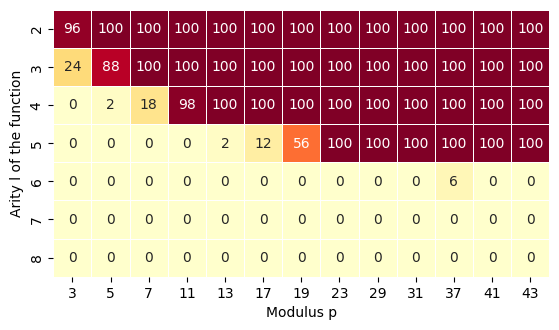
\includegraphics[]{img/p_encodings/heatmap_success.png}
    \caption{Rate of success of the algorithm for 100 random Boolean functions for different values of $\ell$ and $p$.}
    \label{fig:heatmap_success}
\end{figure}


Figure \ref{fig:lineplot_timings} shows the evolution of the time of execution of the algorithm for random Boolean functions \emph{for which no solution exists}.  It shows the explosion of the complexity for high values of
$p$, and justifies the need of a more efficient algorithm for those function (we introduce one in Section \ref{sec:graphs}).  


\TODO{Harmoniser l'algorithme suivant (commenté)}
\begin{figure}
    \centering
    \begin{minipage}{0.55\textwidth}
        \centering
        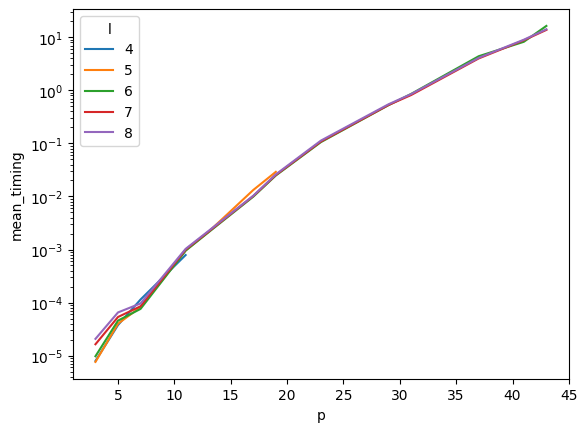
\includegraphics[width=\linewidth]{img/p_encodings/lineplot_timings.png}
        \caption{Running time of the algorithm for different values of $\ell$ and $p$ for random functions. Note that the scale is logarithmic.}        
        \label{fig:lineplot_timings}
        \end{minipage}\hspace{0.04\textwidth}
    \begin{minipage}{0.35\textwidth}
        \centering
        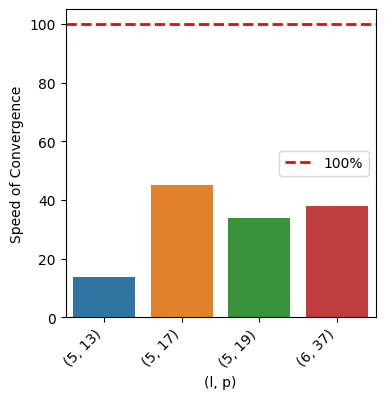
\includegraphics[width=\linewidth]{img/p_encodings/barplot.png}
        \caption{Ratio between the time to find a solution when it exists with the time to run the full algorithm when no solution exists.}
        \label{fig:barplot_ratio}
    \end{minipage}
    \caption{Some metrics about running time.}
    \label{fig:overall}
\end{figure}
Lastly, Figure \ref{fig:barplot_ratio} shows how long it takes to find a solution when one exists, relatively to the running time when no solution exist at all. It illustrates a form of "speed of convergence" and shows that it is located around $\frac{1}{3}$.



    
\subsection{An Efficient Sieving Heuristic to Find Suitable Encodings}
\label{sec:heuristic_matthieu}


Let us consider a function $f: \B^\ell \mapsto \B$ of matrix of constraints $C=(C_j^{(i)})_{\substack{1 \le i \le n_j\\1 \le j \le \ell}}$ and its associated system of linear inequalities:

$$
\left \{
\begin{array}{c}
     c_1^{(1)} \times d_1 + c_2^{(1)} \times d_2 + \dots + c_\ell^{(1)} \times d_\ell   \neq 0 \mod p\\
     c_1^{(2)} \times d_1 + c_2^{(2)} \times d_2 + \dots + c_\ell^{(2)} \times d_\ell \neq 0 \mod p\\
    \dots
\end{array}
\right .
$$


The principle is to sample random values in $\Z$ (with some large bound) and affect them to the $d_j$'s. If all the corresponding values for all the $C_i = \sum_{j=1}^{\ell} c_j^{(i)} \times d_j$ are not divisible by a value $p$, then the vector $(d_j \mod p \mid j \in \{1, \dots, \ell\})$ is a solution of the system of inequalities generated by $C$. 


To reduce the amount of samples required to find a solution, we want to avoid sampling trivially wrong sets of $d_j$'s. For example, if all the $d_j$'s are themselves divisible by $p$, then the $C_i$'s will all be divisible as well. To tackle this problem, we perform the sampling across \emph{prime numbers in $\Z$}.



%\begin{algorithm}
%    \caption{Sample a solution $\vec d$ in $\Z$ for a function $f$ and returns a possible value for $p$.}
%    \label{alg:heuristic_matthieu}
%    \begin{algorithmic}
%    \Require \\
%    $\{C_i\}_{1 \le i \le n}$ \Comment{The lines of the matrix of constraints $C$ of the function $f$ } \newline
%    $P$ \Comment{The sets of possible values for $p$ to be tested} \newline
%    $D$ \Comment{The sets of possible values in $\Z$ to assign to the $d_i$'s. All these elements are big primes}
%    \Ensure $f$ is possible to evaluate using a modulus smaller or equal than $p$.
%    \State{$\vec{d} \drawfrom D$} \Comment{Sample random prime values in $\Z$ and assign it to $\Vec{d} = (d_1, \dots, d_l)$}
%    \State{$\vec r = C \times \vec{d}$}  \Comment{$\vec r$ is the right member of the system}
%    \For {$p \in P$}
%        \If{$0 \in [\Vec{r}]_p$}          \Comment{If $p$ divides one of the coordinates of $\vec r$}
%            \State{$P \gets P \setminus \{p\}$} \Comment{This value of $p$ is incorrect}
%        \EndIf
%    \EndFor
%    \If{$\mid P \mid > 0$}
%        \State{\Return{$\min(P)$}} \Comment{Returns the smallest possible value for $p$, if any.}
%    \EndIf   
%    \end{algorithmic}
%\end{algorithm}


Running this algorithm several times and keeping the smallest returned value for $p$, one gets an upper bound on the minimum $p$ required to evaluate a function with our framework. Note that, on the contrary of the deterministic search algorithm, this heuristic does not require a prime $p$.


\paragraph{Example:} Let us consider the s-box of the block cipher ASCON. We study this s-box in more details and provide an exact optimized solution for its homomorphic evaluation in Section \ref{sec:ascon}. Here, we apply Algorithm \ref{alg:heuristic_matthieu} on the five functions generating the five output bits and monitor the results until we gather $N=10000$ non-zero possible values for $p$.


The figure \ref{fig:ascon_0_p_frequencies} shows the repartition of the returned values of $p$ by the algorithm during these $N$ runs on the first subfunction. The optimal value of $p$ found by the deterministic approach of Section \ref{sec:search_algorithm} is $17$ so the upper bound $19$ is pretty close, despite being rarely found by the algorithm. Also, the figure \ref{fig:ascon_0_count_iter} shows $21$ (the second best solution found by the sieving) is almost instantly found by the algorithm.


\begin{figure}
  \begin{minipage}{0.48\linewidth}
    \    \centering
    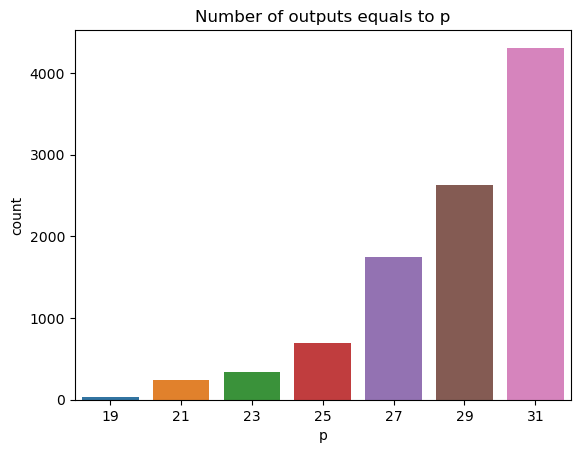
\includegraphics[width=\linewidth]{img/p_encodings/heuristic_ascon_0_p_frequencies.png}
    \caption{The outputs of $10000$ runs of the Algorithm \ref{alg:heuristic_matthieu} for the first subfunction of the Ascon s-box}
    \label{fig:ascon_0_p_frequencies}
  \end{minipage} \hfill
  \begin{minipage}{0.48\linewidth}
    \centering
    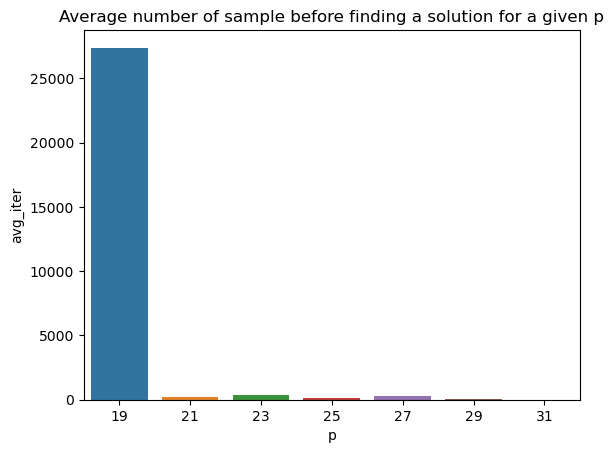
\includegraphics[width=\linewidth]{img/p_encodings/heuristric_ascon_0_count_iter.png}
    \caption{Number of iterations required to get a solution for a given value of $p$}
    \label{fig:ascon_0_count_iter}
  \end{minipage}
\end{figure}


In the process of finding the smallest $p$ possible and a correct vector of $p$-encoding to evaluate a function $f$, this heuristic is really efficient to get a tight upper bound on the value of $p$.


\section{Scaling our Approach to any Boolean Circuit}
\label{sec:p_encodings_graphs}

Our framework optimizes the homomorphic evaluation of single Boolean functions but suffers the following limitations:

\begin{enumerate}
    \item For a Boolean function with a high number of inputs, the search algorithm may be very time-consuming.
    \item Some functions simply do not have any solution for acceptable values for $p$ ($p < 32$ for example) and thus are not efficiently evaluable in a single PBS.\footnote{The PBS can be evaluated for larger values of $p$ but it quickly becomes inefficient as $p$ grows.}
\end{enumerate}


As a consequence, we need a solution to extend our framework to these cases. In this section, we propose a strategy to leverage the circuit representation of a ``tough'' function $f$ to find a strategy of homomorphic evaluation with as few bootstrappings as possible.


\subsection{Graph of Subcircuits}
\label{sec:graph_definition}

Let $f: \B^\ell \longrightarrow \B$ be a Boolean function, and let $\mathcal{F}$ be a Boolean circuit representing $f$ (some preliminaries about Boolean circuits can be found in Section \ref{sec:p_encodings_preliminaries_boolean}). Let us describe the layout of the circuit $\mathcal{F}$. It has $\ell$ input wires, denoted by $\{y_j\}_{1 \le j \le \ell}$, and the output wire is denoted by $z$. The intermediary wires are denoted by $\{t_j\}_{1 \le j \le \theta}$. The Boolean operation gates are of fan-out 1. 


Our goal is to split the circuit into a directed acyclic graph $\mathcal{G}$, whose vertexes are subcircuits $\{\mathcal{F}_1, \dots, \mathcal{F}_k\}$ and whose edges connect the outputs of a subcircuit with the input of another. Each subcircuit $\mathcal{F}_i$ represents a subfunction $f_i: \B^{l_i} \mapsto \B$ that is evaluable with a gadget with our framework. 

We use the same notations to refer to the elements of a subcircuit $\mathcal{F}_i$ and we index them with $i$. The output of $\mathcal{F}_i$ is denoted by $z^{(i)}$ and its inputs by $\{y_j^{(i)}\}_{1 \le j \le \ell}$ and so on. 


The graph is valid for $f$ with respect to modulus $p$ if the following properties are satisfied:
\begin{itemize}
    \item Each subcircuit $\mathcal{F}_i$ has only one output $z^{(i)}$.
    \item For a subcircuit $\mathcal{F}_i$, all its inputs are either inputs of the whole circuit or outputs of other subcircuits of the graph. We can write this property as:
    $$
    \{y_j^{(i)}\}_{1 \le j \le l_i} \subset \left ( \{y_j\}_{1 \le j \le \ell} \cup \{z^{(j)}\}_{1 \le j < i} \right )
    $$
    Thus, the indexing of the $\mathcal{F}_i$'s respects the topological order of the graph, i.e. no gates of $\mathcal{F}_i$ has a child in any of the $\mathcal{F}_j$, with $j < i$.
    \item All the Boolean functions $f_i$ represented by the subcircuits $\mathcal{F}_i$ are evaluable in a single bootstrapping with modulus $p$ with our proposed method. 
    \item The last subcircuit $\mathcal{F}_c$ of the graph has $z$ (the output of the main circuit) for output: $z^{(c)} = z$.
\end{itemize}

\begin{figure}
    \centering
    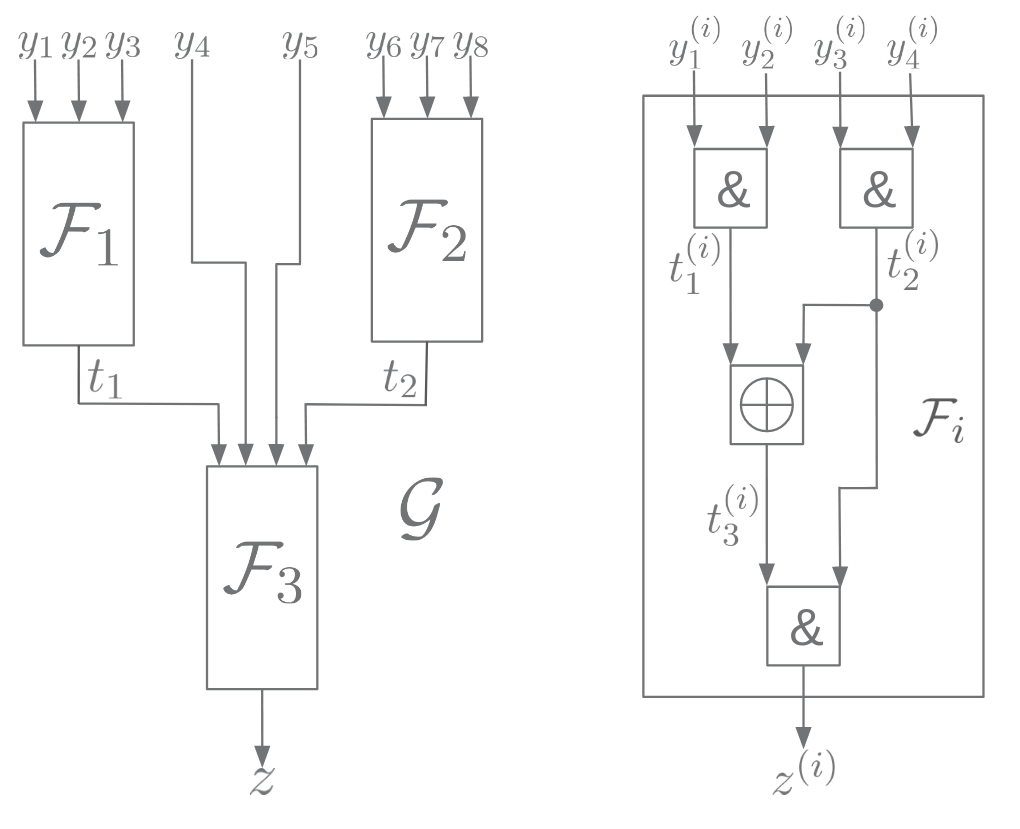
\includegraphics[width=0.75\textwidth]{img/to_harmonize/graphs.png}
    \caption{Example of graph of subcircuits (on left) and of a valid subcircuit (on right). Each subcircuit $\mathcal{F}_i$ is evaluated homomorphically with a gadget $\Gamma_i$.}
    \label{fig:enter-label}
\end{figure}




To homomorphically evaluate the function $f$, we evaluate each subcircuits with one bootstrapping for each of them and get the final result. In order to reduce the cost of evaluation for a given $p$, the goal is hence to find the \emph{smallest} valid graph possible in terms of number of subcircuits. Taking a greater value of $p$ produces a different graph that may be smaller (as subcircuits might be larger), but the timings of bootstrapping in this graph might on the other hand be greater. One can therefore run the search for different values of $p$ and keep the most efficient setup among the possible graphs. %Additionally, for some values of $p$, such a graph may not exist.

\subsection{Heuristics to Find a Small Graph}
\label{sec:heuristics_graph}

Finding such a graph can be done by exhaustively evaluating all the possible subcircuits with our method introduced in Section \ref{sec:p_encodings_search}, and then find the more efficient one. However it is not really practical to evaluate \emph{all} the possible subcircuits, so we develop some heuristics to reduce the search space. Let us start by defining a few bounds on the considered subcircuits, we will leave the other ones apart in our algorithm:

\begin{itemize}
    \item The subcircuits have at most $B$ inputs ($\forall i, l^{(i)} < B$). The purpose of this bound is to limit the running time of Algorithm \ref{alg:add_element}. In practice, for our experiments, we took $B = 10$.
    \item The subcircuits are evaluable with one single bootstrapping with a maximum value $p_{max}$. This value ensures a bootstrapping with a reasonable timing. If the search algorithm fails for $p_{max}$, the subcircuit is dropped without trying to extend $p$. In our experiment, we took $p_{max}=31$.
\end{itemize}


In order to decompose our Boolean circuit into a graph satisfying the above property for a modulus $p$, we would want to exhaustively search all the subcircuits of $\mathcal{F}$ compliant with the bounds we introduced earlier. However, all subcircuits are not equally worth to evaluate. In particular a wire incoming a copy gate is particularly worth evaluating because is costs one bootstrapping but produce several inputs for the next subcircuits. 

We gather wires that precede a copy gate in the set $\mathcal{Z}$. We add to this set the global output $z$. We also gather the input wires of the global circuit $\mathcal{F}$ in the set $\mathcal{Y}$. We define the notion of \textit{atomic subcircuit} that is a valid subcircuit whose all inputs belong to $\mathcal{Y} \cup \mathcal{Z}$ and whose output belongs to $\mathcal{Z}$. Note that the merge of two atomic subcircuits that respect the global circuit wiring is also an atomic subcircuit.

\medskip

Our heuristic works as follows:

\begin{enumerate}
    \item For each of these outputs $z_i \in \mathcal{Z}$, we exhaustively construct a set $\widehat{\mathcal{F}_{z_{i}}}$ that gathers all the atomic subcircuits whose output is $z_i$.
    We then filter out the subcircuits of $\widehat{\mathcal{F}_{z_{i}}}$ that do not comply with the bounds introduced at the beginning of the section or that are not evaluable with a gadget with the input modulus $p$ (we use Algorithm \ref{alg:add_element} to decide that).
    \medskip
    \item Now we want to construct the smallest valid graph evaluating $\mathcal{F}$ using subcircuits from the $\widehat{\mathcal{F}_{z_{i}}}$'s. While finding the smallest graph is hard, constructing any valid graph is easy. As a consequence, our strategy to find a small graph is to randomly create a lot of valid graphs and to take the smallest one. The procedure to create a valid graph is the following: we start from the output $z$ and we randomly draw a subcircuit $\mathcal{F}_z$ from $\widehat{\mathcal{F}_z}$. The inputs of $\mathcal{F}_z$ can be sorted into two categories: the ones belonging to $\mathcal{Y}$ and the ones belonging to $\mathcal{Z}$. For each one of these latter wires $w \in \mathcal{Z}$, we repeat the procedure, i.e. we draw a subcircuit $\mathcal{F}_w$ from $\widehat{\mathcal{F}_w}$, and so on. When we have reached all the input wires of $\mathcal{F}$, we get a valid graph $\mathcal{G}$ . This second step is run a large amount of times (the number of trials is a parameter of the method), and the smallest graph, i.e. the one with the fewest subcircuits, is returned.
\end{enumerate}

We carried on this method on the s-box of AES in Section \ref{sec:p_encodings_aes}.

\subsection{Parallelization of the Execution of the Graph}
\label{sec:parallelization}

Once we have our graph $\mathcal{G}$, we can identify its $n_\mathcal{L}$ \emph{layers}. Formally, they are defined as:

\begin{definition}
    A layer $\mathcal{L}$ of a graph $\mathcal{G}$ is a set of subcircuit $\{\mathcal {F}_\alpha, \dots, \mathcal{F}_\omega\}$ of $\mathcal{G}$ that verifies: $\forall \mathcal{F}_i, \mathcal{F}_j \in \mathcal{L}, \mathcal{F}_i \text{ is not an ancestor node of } \mathcal{F}_j.$    
\end{definition}

By construction, all the subcircuits belonging to the same layer can be evaluated in parallel. This reduces the number of bootstrapping steps from $k$ (the number of subcircuits in the graph $\mathcal{G}$) to $n_\mathcal{L}$ (the number of layers). Our graph-finding heuristic can be tweaked to select the graph with minimum number of layers instead of minimum number of subcircuits to optimize parallelization.

\section{Adaptation of TFHE and the \texttt{tfhe-rs} Library}
\label{sec:TFHE_adaptation}

From a high level point of view, our technique can be seen as adding an additional layer of abstraction on top of TFHE. However things are not that simple: picking odd values for $p$ leads to some changes in the inner working of the programmable bootstrapping (PBS), and the choice of parameters is also affected by this change. Moreover, we implemented our framework by forking the \texttt{tfhe-rs} library~\cite{tfhe-rs} written in Rust. The following section covers the adaptation of the PBS and the choice of new parameters. The adaptation of the library is treated in Section \ref{sec:library}.

\subsection{Dealing with the Negacyclicity Problem for an Odd $p$}
\label{sec:solving_negacyclicity}

In the following, we explain the negacyclicity problem and how we propose to solve it. To do so, we need to dig into the details of the \texttt{BlindRotate} step of the PBS, that we have introduced in Section \ref{sec:bootstrapping}.

Let $v(X)$ be a polynomial of the ring $\Z_{q, N}[X]/(X^N+1)$, denoted by $v(X) = \sum_{k=0}^{N-1} v_k X^k$. Observe that a multiplication by $X$  in this ring ``rotates'' the coefficients of the polynomial: \[X \cdot v(X) = - v_{N - 1} + v_0 \cdot X \dots + v_{N - 2} X^{N - 1}~.\]

In TFHE, the polynomial multiplication in the blind rotation is actually done by $X^{-\Tilde{\mu}}$, with $\Tilde{\mu} = \rounding{\frac{\mu \cdot 2N}{q}}$, which lives in $\{0, \dots, 2N - 1\}$. This leads to two problems:

\begin{itemize}
    \item A coefficient $v_j$ can be brought in first place by two differents rotations: the one induced by the polynomial multiplication by $X^{\modulo{-j}{2N}}$ and the one by $X^{[-j + N]_{2N}}$.
    \item Each time a coefficient goes last to first, it gets negated (because $X^N = -1$ in the ring). So actually, the multiplication by $X^{[-j]_{2N}}$ yields correctly $v_j$, but the one by $X^{[-j + N]_{2N}}$ yields $-v_j$.
\end{itemize}


However, these problems can be circumvented for even and odd values of $p$. Recall that $\mu = m + e \in \Z_q$, with $e$ sampled from a small centered Gaussian. The use of a small error makes that $\mu$ does not take all the values of $\Z_q$ with the same probability: in particular, the densest parts in terms of probability over $\Z_q$ are the one close to the ``unscrambled'' values of $m$, namely $\left \{ \rounding{\frac {k q}{p}} \mid k \in \Z_p \right \}$. We illustrate this distribution on Figure \ref{fig:density_of_phase}. We call these sections of the torus the \emph{dense spots}.


\begin{figure}
    \begin{subfigure}{0.49\linewidth}
        \centering
        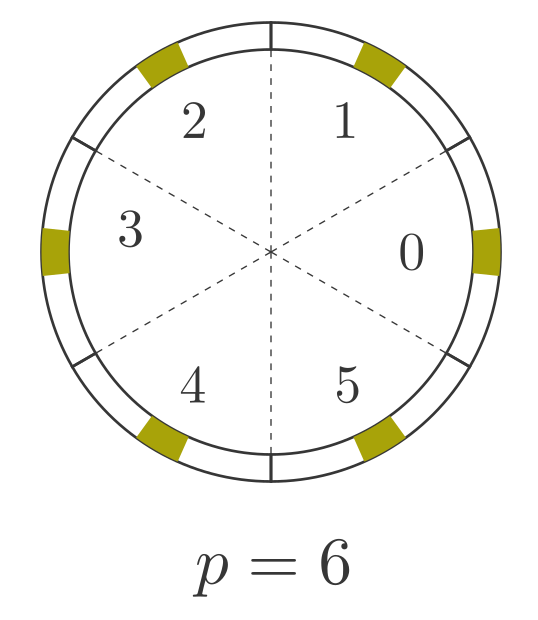
\includegraphics[width=0.5\linewidth]{img/to_harmonize/busy_sectors_2.png}
    \end{subfigure}\hspace{1em}% Adjust the margin width as needed
    \begin{subfigure}{0.49\linewidth}% Specify the width here
        \centering
        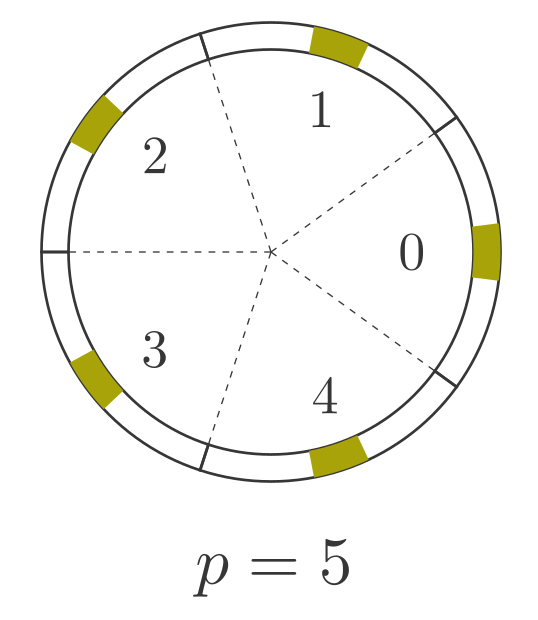
\includegraphics[width=0.5\linewidth]{img/to_harmonize/busy_sectors.png}
    \end{subfigure}
    \caption{Distribution of the values of $\mu$ across $\Z_{q}$ for $p = 6$ and $p = 5$: the colored parts show the dense spots where the value has a high probability to lie in. The width of these sectors depends on $\sigma$ (the standard deviation of the error distribution $\chi$ of TFHE). Note that this repartition looks the same for $\Tilde{\mu}$ in $\Z_{2N}$.}    
    \label{fig:density_of_phase}
\end{figure}


When we transpose these dense spots into $\Z_{2N}$, they become the sectors close to $\left \{ \rounding{\frac{k \cdot 2N}{p}} \mid k \in \Z_p \right \}$. Let us note that the noises in $\Z_q$ and $\Z_{2N}$ are fundamentally different: the former is the one added at encryption that may have grew during the homomorphic computations, and the latter is called ``drift'' and is caused by the accumulation of the rounding errors on each coefficient of the ciphertext during the modulus switching (but this difference in nature does not impact our purpose). 
Let $k \in \Z_p$, the multiplication $X^{- \frac{k \cdot 2N}{p}} \cdot v(X)$ yields the same degree-zero coefficient as the multiplication  $X^{\modulo{- \frac{k \cdot 2N}{p} + N}{2N}} \cdot v(X)$, up to the minus sign. For the sake of clarity, we write the exponent of the latter in a slightly different manner: 
\[\modulo{
    \frac{
        -k \cdot 2N
        }
    {
        p
    }
    + N
}{2N} = 
\modulo{
    \frac{
    (-k + \frac p 2 ) \cdot 2N
    }
    {p}
}
{2N}\]


This is where the parity of $p$ plays a part: if $p$ is even, then $\modulo{
    \frac{
    (-k + \frac p 2 ) \cdot 2N
    }
    {p}
}
{2N}$ is a dense spot as well. So, the rotations by these two values will happen with high probability and they will both yield the same coefficient $v_{\frac{k \cdot 2N}{p}}$ (up to the minus sign for one of them). Thus, when evaluating a function $f$ with a PBS, the calls $f(k)$ and $f(k + \frac p 2)$ will produce the same output (one again, up to the minus sign), which is a collision constraining the definition of $f$. On the other hand, let us consider an odd value for $p$. Then, $\modulo{
    \frac{
    (-k + \frac p 2 ) \cdot 2N
    }
    {p}
}{2N}$ is no longer a dense spot, as it lies exactly halfway between the two dense spots $\modulo{
    \frac{
    (-k + \frac {p-1} {2} ) \cdot 2N
    }
    {p}
}{2N}$ and $\modulo{
    \frac{
    (-k + \frac {p+1} {2} ) \cdot 2N
    }
    {p}
}{2N}$. As a consequence, collision never occurs. Figure \ref{fig:torus_p_even_vs_odd} illustrates this phenomenon.


\begin{figure}
  \begin{subfigure}{0.49\linewidth}
    \    \centering
    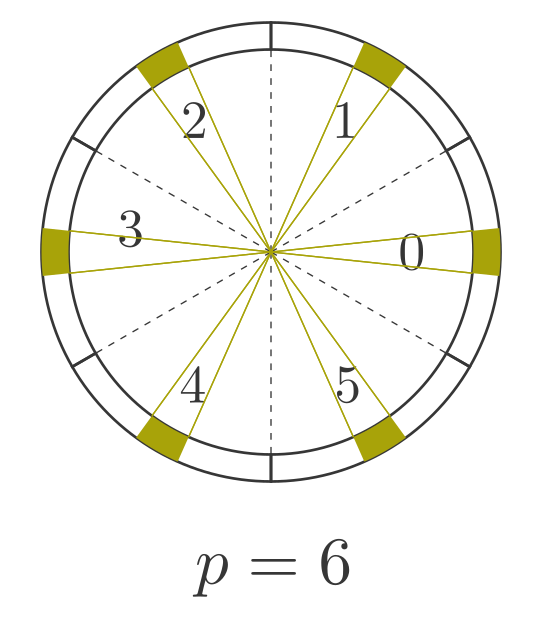
\includegraphics[width=0.5\linewidth]{img/to_harmonize/torus_p_even.png}
    \caption{With $p$ even, the dense spots of each half of the torus are aligned.}
    \label{fig:torus_p_even}
  \end{subfigure}\hspace{1em}% Adjust the margin width as needed
  \begin{subfigure}{0.49\linewidth}
    \centering
    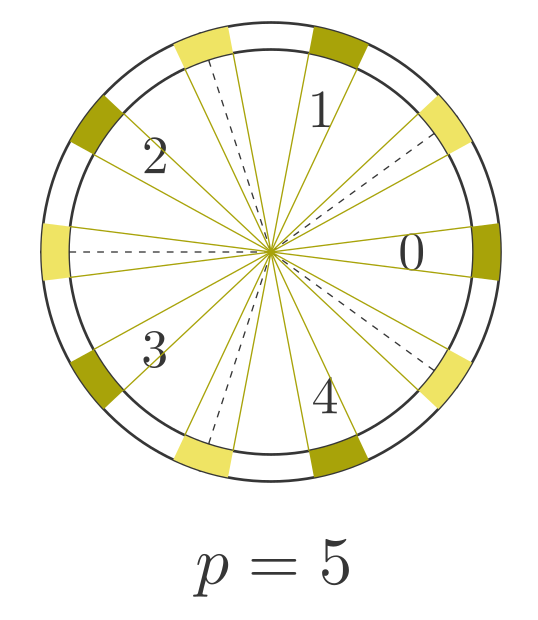
\includegraphics[width=0.5\linewidth]{img/to_harmonize/torus_p_odd.png}
    \caption{With $p$ odd, the dense spots face empty spots, close to the bounds of the $p$-sectors.}
  \end{subfigure}
  \caption{}
  \label{fig:torus_p_even_vs_odd}
\end{figure}



That is why we select only odd values for $p$ in our framework. 


We will see in Section \ref{sec:parametrization} how this change impacts the parametrization of the scheme.

\TODO{Ecrire que ça ne chanre rien au paramétrage, avec une référence sur la bonne section}






\paragraph{Exception for $p=2$:} We just said that only odd values can be selected for $p$ in our framework, however $p$-encodings with even values of $p$ exist as well: nonetheless they need to achieve the relaxed negacyclicity property introduced in Definition \ref{def:encoding}. This restriction makes them basically useless, as using only odd $p$-encodings is sufficient to evaluate all possible Boolean functions without having to bother with the negacyclicity property. However, the case $p=2$ is an exception: the valid $2$-encodings are automatically negacyclic and allow to evaluate the \texttt{XOR} operation by simply performing an homomorphic sum (so without bootstrapping). So it might be efficient to switch between $2$-encodings for \texttt{XOR} operations and $p$-encodings (with odd $p$) for non-linear Boolean functions. We make use of this strategy in our implementation of the Keccak permutation in Section \ref{sec:keccak} and for the AES in Section \ref{sec:aes}.



\subsection{Construction of the Accumulator for an Odd $p$}
\label{sec:accumulator}


The accumulator is the polynomial $v(X)$ used in the \texttt{BlindRotate} step of the PBS. In the Section \ref{sec:solving_negacyclicity}, we showed how the values are spread over the torus after bootstrapping. To actually make that works, we need to explicitly characterize this polynomial. In the following presentation, we neglect roundings to keep notations light (as if $p$ would divide $N$), or, equivalently, the division operator is assumed to include rounding.

\begin{definition}
    If $p$ is an odd modulus, and $f: \Z_p \mapsto \Z_{p'}$ a function, then the accumulator $v(X) \in \Z_{N, q}[X]/(X^N+1)$ has the form:\[v(X) = X^{- \frac {N} {2p}} \cdot \sum_{j=0}^{N/p - 1} X^j  \cdot \left ( \sum_{i=0}^{\frac{p-1}{2}} f(i) X^{i \frac{2N}{p}} + \sum_{i=0}^{\frac{p-1}{2} - 1} -f \left (i + \frac{p+1}{2} \right ) X^{i \frac{2N}{p} + \frac N p} \right )\]
\end{definition}


Let us explain the structure of this accumulator. The polynomial has degree $N$ and is made of $p$ distinct windows of width $\frac{N}{p}$. Each of these windows has constant coefficient value $f(k)$, for $k \in \{0, \dots, p-1\}$.
For $0 \le \alpha \le \frac{p-1}{2}$, the range of degrees whose coefficients are $f(\alpha)$ is $\left [ \alpha \frac{2N}{p} - \frac{N}{2p}~;~ \alpha \frac{2N}{p} + \frac{N}{2p} \right ]$. Now, for $\frac{p+1}{2} \le \beta \le p-1$, we can write $\beta = \alpha + \frac{p+1}{2}$, with $0 \le \alpha < \frac{p-1}{2}$. This time, the range of spanned degrees is $\left [ \alpha \frac{2N}{p} + \frac{N}{2p} ~;~ (\alpha + 1) \frac{2N}{p} - \frac{N}{2p} \right ]$. Thus, the values $k \in \{0, \dots, p-1\}$ spans the entire space $[0; N)$ without overlap. The values over $\frac{p+1}{2}$ gets negated by the negacyclicity, so the underlying coefficient is also negated to compensate this effect. We illustrate this construction on Figure \ref{fig:accumulator}.

\begin{figure}
    \centering
    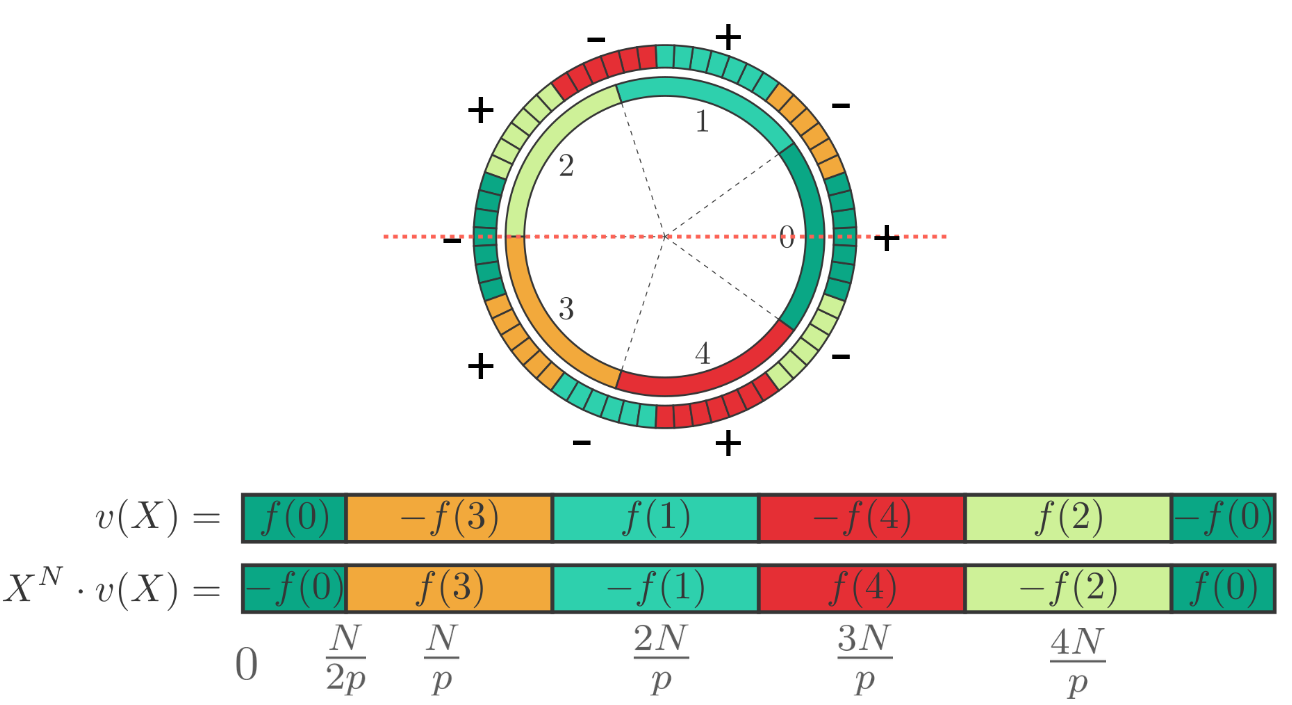
\includegraphics[width=\textwidth]{images/accumulator.png}
    \caption{Illustration of the construction of the accumulator. On top is the ring $\Z_{2N}$ splitted in windows. Below is a representation of the polynomial $v$, with its version once rotated by a multiplication by $X^N$. On the figure, $p$ = 5.}
    \label{fig:accumulator}
\end{figure}



\subsection{Crafting of Parameters}
\label{sec:parametrization}
The instances of the TFHE scheme are defined by a set of parameters. These parameters should simultaneously ensure the security of the scheme and the correctness of the homomorphic computations. They also determine the time of execution of one PBS. Here we define a framework to dimension the parameters required to optimally execute a given gadget.

Finding an optimal set of parameters for a given application is a hard problem and has been studied in particular in \cite{zama_parameters_optimization}. The parameters need to ensure three properties: security, correctness and efficiency. 

Let us start by an overview of the different parameters at play in an instance of the TFHE bootstrapping:

\begin{itemize}
    \item $n$: the dimension of the \LWE samples. Namely, the TLWE ciphertexts are vectors of length $n + 1$.
    \item $q$: the modulus of the ring the encrypted values live on. In \texttt{tfhe-rs} those values are stored on \texttt{u32} values, making $q = 2^{32}$. We treat this as an immutable platform-dependent value.
    \item $\sigma$: the standard deviation of the Gaussian distribution of error in \LWE samples.
    \item $k$: the dimension of the \GLWE samples. If $k=1$, we talk about \RLWE samples.
    \item $\sigma'$: the standard deviation of the Gaussian distribution of error in \GLWE samples.
    \item A few more parameters dimensioning some inner algorithms of the bootstrapping. A detailed description and an analysis of their impact on performances and noise level can be found in \cite{zama_parameters_optimization}. In this work, they are denoted as \emph{micro-parameters}.
\end{itemize}

In \cite{zama_parameters_optimization}, authors elaborate a strategy where they define an \textit{atomic pattern} of FHE operators, that is to say a subgraph of FHE operators in which the noise of the output is independent from the one in the inputs. Then, they develop an optimization framework to derive the best set of parameters for a given atomic pattern.

In particular, the first atomic pattern they study, that they denote by $\mathcal{A}^{(CJP21)}$, is a subgraph composed of a linear combination of ciphertexts with clear constants, then a \texttt{Keyswitch} and then a \texttt{BlindRotate} followed by a \texttt{SampleExtract} (\texttt{ModulusSwitch} is seen as a part of \texttt{BlindRotate}). Note that in Section \ref{sec:bootstrapping} we introduced the bootstrapping of TFHE by putting the \texttt{BlindRotate} before the \texttt{Keyswitch}, but the other way around is also doable. To dimension the parameters of TFHE to evaluate such an atomic pattern, their framework takes as input the 2-norm of the vector of constants of the linear combination (denoted by $\nu$) and a noise bound $t$ on the standard deviation of the distribution of error in a ciphertext that ensures a correct decryption with a good probability $(1-\epsilon$). We elaborate further on how this bound is constructed below in this section.

If we look closely, the evaluation of a gadget we introduced in Definition \ref{def:gadget} can be seen as a $\mathcal{A}^{(CJP21)}$ with a few differences. Thus, we slightly modified the tool \texttt{concrete-optimizer} \cite{concrete-optimizer}, that allows to generate parameters for different types of atomic patterns, to support our gadget as a new atomic pattern. Let us dive into the differences between a gadget and a $\mathcal{A}^{(CJP21)}$:

\paragraph{Support of odd values for $p$:} Using an odd value for $p$ changes the bootstrapping procedure, and in particular the definition of the accumulator for the \texttt{BlindRotate} (as explained in Section \ref{sec:accumulator}). With our construction, the windows in the polynomial are half the size of the ones for an even $p$, which impacts the noise bound $t$. 
As this bound depends of the failure probability $\alpha$ that the user is ready to tolerate, we shall denote it $t_\alpha$ hereafter, which satisfies: $t_\alpha = \frac{\Delta}{2z^*(1-\sqrt[N]{1-\alpha})}$
where $z^*$ is the \emph{standard score} and $\Delta$ is the scaling factor (see~\cite{zama_parameters_optimization} for more explanations). The impact of our adaptation on this formula is solely with respect to the scaling factor. In the context of an $\mathcal{A}^{(CJP21)}$, we have $\Delta = \frac{q}{2^\pi p}$ with $\pi$ the number of MSB for padding. As explained in Section \ref{sec:solving_negacyclicity}, we do not need any padding mechanism anymore, so the $2^\pi$ vanishes. However, the length of a window is divided by $2$, and $p$ does not divide $q$ anymore so we need to add a rounding. We finally get $\Delta = \rounding{\frac{q}{2p}}$.


\paragraph{Link between input encodings and $\nu$:} In a scenario where only one gadget has to be evaluated, its inputs are freshly encrypted ciphertexts. Then, there is no need to perform any encoding switching before evaluating the gadget, and so we are in the context of a $\mathcal{A}^{(CJP21)}$ with $\nu = 1$. However, if we are in a context of a \textit{graph} of gadgets like in Section \ref{sec:graphs}, the output of a gadget can be used as input of subsequent gadgets under different encodings. In this case, some encoding switchings are necessary. If these encoding switching are made using a mutiplication by a constant (Property \ref{prop:mult_constant}), we are still in the context of a $\mathcal{A}^{CJP21}$ but with $\nu \ne 1$. 
To formalize that, we first recall that Algorithm \ref{alg:add_element} produces gadgets of the form $\Gamma = \left (\vec{\Encoding_{in}}, \Encoding_{out}, p_{in}, p_{out}, f \right )$, with $\Encoding_{in}^{(i)} = \EncDefOne{d_i}$. Thus, if we fix that all gadget output ciphertexts are encoded under $\Encoding_{out} = \EncDefOne{1}$, then the encoding switchings needed before an evaluation of $\Gamma$ corresponds to a linear combination of the inputs with the vector $\vec d = (d_i \mid i \in [1, \ell])$, so we fall back on a $\mathcal{A}^{(CJP21)}$ with $\nu = \customnorm{\vec d}$.


We implemented these changes in \texttt{concrete-optimizer} and uses it to generate sets of parameters for our implementations detailed in Section \ref{sec:implementations}.

\subsection{Concrete Implementations of $p$-Encodings and Homomorphic Functions in \texttt{tfhe-rs}}
\label{sec:library}


To implement our framework, we relied on the $\texttt{tfhe-rs}$ library~\cite{tfhe-rs}. Here is a list of the major changes we applied to the code:

\paragraph{Addition of the notion of $p$-encoding: } An encoding $\Encoding$ is simply implemented with a structure \texttt{Encoding} storing two \texttt{HashSets} and the modulus $p$. The \texttt{HashSets} represent both sets $\Encoding(0)$ and $\Encoding(1)$. When creating an \texttt{Encoding}, the code checks whether the two underlying sets are disjoint or not. Moreover, the operation of encryption and decryption are modified as well. The signatures change from:\[\texttt{encrypt(Boolean, ClientKey) -> Ciphertext}\] to: \[\texttt{encrypt(Boolean, ClientKey, Encoding) -> Ciphertext}\] (same for \texttt{decrypt}). The functions also perform the mapping $\B \mapsto \Z_p$ before encryption and the other way around after decryption.


\paragraph{Support of odd moduli: } The native \texttt{tfhe-rs} only support power-of-two-moduli $p$. We extended the library to handle odd values for $p$. This required modifying the encryption and decryption algorithm, and to compute the sets of parameters with the method of Section \ref{sec:parametrization}.


\paragraph{Definition of the new structure $\texttt{Gadget}$: } According to the evaluation strategy we introduced in Section \ref{sec:new_strategy}, we wrote a new structure $\texttt{Gadget}$, associated to a Boolean function $f: \B^\ell \mapsto \B$, carrying:
\begin{itemize}
    \item A list of the \texttt{Encoding} objects for the inputs: $\Encoding_{in} = (\Encoding_1, \dots, \Encoding_l)$, with the input modulus $p_{in}$ they encoded on.
    \item The output \texttt{Encoding} object $\Encoding_{out}$, with the output modulus $p_{out}$ it is encoded on.
    \item The clear function $f$.
\end{itemize}
When such a structure is constructed, it self-checks whether $f(\Encoding_{in})$ is valid. Then, when provided $\ell$ $\texttt{Ciphertexts}$ objects encoded under their respective $p$-encoding, it executes the homomorphic sum and the PBS and outputs the results encoded under $\Encoding_{out}$. Some utilitary functions performing encoding-switching are also available, allowing the chaining of several $\texttt{Gadget}$.


\paragraph{Implementation of the accumulator: } The procedure of bootstrapping of \texttt{tfhe-rs} is slightly modified to support the new version of the accumulator we introduced in Section \ref{sec:accumulator}.

\paragraph{Parsing of graphs: } We implemented a Python script that produces graphs to represent more complex functions that requires several PBS, as described in Section \ref{sec:graphs}. These graphs are stored with a comprehensive file format and our Rust implementation has a module of parsing allowing to load these graphs and automatically generate the corresponding graph of \texttt{Gadget}.





\section{Application to Cryptographic Primitives}
\label{sec:p_encodings_implementations}


In this section, we apply our approach on some cryptographic primitives. For each primitive, we first explain the construction of the gadgets required and report the concrete performances of our implementation. We detailed all the timings of our experimentations along with the sets of parameters we used in Section \ref{sec:tables_perfs}.

For performance measurement, we implemented our framework in our fork of the library \texttt{tfhe-rs} \cite{tfhe-rs} adapted as discussed in Section \ref{sec:TFHE_adaptation} and we generated the sets of parameters thank to our version of \texttt{concrete-optimizer} \cite{concrete-optimizer}. By default, we tailored the sets of parameters to limit the probability of failure $\epsilon$ of a bootstrapping to $2^{-40}$, and a security level of $\lambda = 128$ bits. All experiments have been carried out on a laptop with a 12th Gen Intel(R) Core(TM) i5-1245U CPU with 10 cores and a frequency of 4.4 GHz, and 16 GB of RAM.


\subsection{SIMON Block Cipher}
\label{sec:simon}

SIMON is a hardware-oriented block cipher developed in \cite{simon}, which relies only on the following operations: \texttt{AND}, rotation, \texttt{XOR}. It is a classical Feistel network for which the Feistel function consists in applying basic operations on the branch, xoring the subkey and then xoring the result with the other branch as depicted in the Figure~\ref{fig:simon_cipher} (on this figure, $S^i$ denotes the left circular shift by $i$ bits.). We use one ciphertext per bit so the rotation operation is essentially free. Note that the key is considered as a plaintext, which does not change anything in the framework. In our implementation, we considered a (128-128) instance of SIMON (i.e. the whole state and the key are of size 128). 


% \begin{wrapfigure}{r}{5.5cm}
% 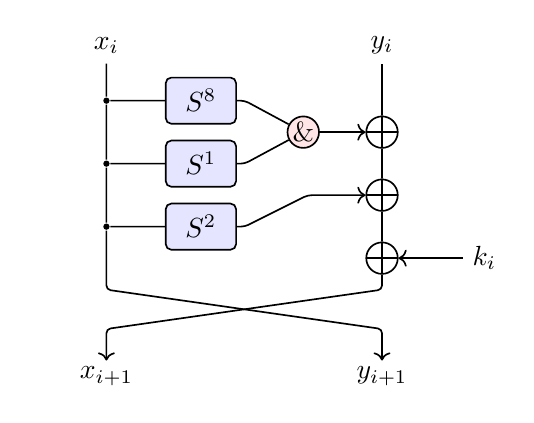
\begin{tikzpicture}
  [line width=0.6,trim left,
   shiftbox/.style = {
     draw, fill=blue!10, rounded corners=2pt,
     inner xsep=0.25cm, inner ysep=0.15cm,
   },
   wire/.style = {
     rounded corners=1.5pt
   },
   xor/.style = {
     draw, circle, inner sep=0cm, minimum size=0.4cm,
     append after command = {
       [shorten >=\pgflinewidth, shorten <=\pgflinewidth,]
       (\tikzlastnode.north) edge (\tikzlastnode.south)
       (\tikzlastnode.east) edge (\tikzlastnode.west)
     }
   },
   odot/.style = {
     draw, circle, inner sep=0cm, minimum size=0.4cm,fill=red!10
   },
   dot/.style = {
     fill, circle, inner sep=0cm, minimum size=0.08cm
   }]

  %Draw nodes
  \node at (1,6.7) (xin) {$x_i$};
  \node at (4.5,6.7) (yin) {$y_i$};
  \node[dot] at (1,6) (d1) {};
  \node[dot] at (1,5.2) (d2) {};
  \node[dot] at (1,4.4) (d3) {};
  \node[shiftbox] at (2.2,6) (S1) {$S^8$};
  \node[shiftbox] at (2.2,5.2) (S2) {$S^1$};
  \node[shiftbox] at (2.2,4.4) (S3) {$S^2$};
  \node[xor] at (4.5,5.6) (x1) {};
  \node[xor] at (4.5,4.8) (x2) {};
  \node[xor] at (4.5,4.0) (x3) {};
  \node[odot] at (3.5,5.6) (AND) {\&};
  \node at (5.8,4.0) (k) {$k_i$};
  \node at (1, 2.5) () {$x_{i+1}$};
  \node at (4.5, 2.5) () {$y_{i+1}$};

  %Draw wires
  \draw[wire] (d1) -- (S1)  (S1.east) -- +(0.1,0) -- (AND);
  \draw[wire] (d2) -- (S2)  (S2.east) -- +(0.1,0) -- (AND);
  \draw[wire,->] (AND) -- (x1);
  \draw[wire,->] (d3) -- (S3) (S3.east) -- +(0.1,0) -- ++(0.9,0.4) -- (x2);
  \draw[wire,->] (xin) -- (d1) -- (d2) -- (d3)
                  -- ++(0,-0.8) -- ++(3.5,-0.5) -- ++(0,-0.4);
  \draw[wire,->] (yin) -- (x1) -- (x2) -- (x3)
                 -- ++(0,-0.4) -- ++(-3.5,-0.5) -- ++(0,-0.4);
  \draw[wire,->] (k.west) -- (x3);
\end{tikzpicture} 
%    \caption{One Feistel round of SIMON. }   
%    \label{fig:simon_cipher}
% \end{wrapfigure}

\begin{figure}
    \centering
    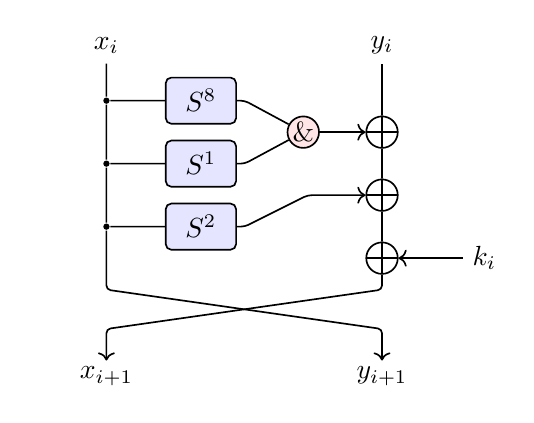
\begin{tikzpicture}
  [line width=0.6,trim left,
   shiftbox/.style = {
     draw, fill=blue!10, rounded corners=2pt,
     inner xsep=0.25cm, inner ysep=0.15cm,
   },
   wire/.style = {
     rounded corners=1.5pt
   },
   xor/.style = {
     draw, circle, inner sep=0cm, minimum size=0.4cm,
     append after command = {
       [shorten >=\pgflinewidth, shorten <=\pgflinewidth,]
       (\tikzlastnode.north) edge (\tikzlastnode.south)
       (\tikzlastnode.east) edge (\tikzlastnode.west)
     }
   },
   odot/.style = {
     draw, circle, inner sep=0cm, minimum size=0.4cm,fill=red!10
   },
   dot/.style = {
     fill, circle, inner sep=0cm, minimum size=0.08cm
   }]

  %Draw nodes
  \node at (1,6.7) (xin) {$x_i$};
  \node at (4.5,6.7) (yin) {$y_i$};
  \node[dot] at (1,6) (d1) {};
  \node[dot] at (1,5.2) (d2) {};
  \node[dot] at (1,4.4) (d3) {};
  \node[shiftbox] at (2.2,6) (S1) {$S^8$};
  \node[shiftbox] at (2.2,5.2) (S2) {$S^1$};
  \node[shiftbox] at (2.2,4.4) (S3) {$S^2$};
  \node[xor] at (4.5,5.6) (x1) {};
  \node[xor] at (4.5,4.8) (x2) {};
  \node[xor] at (4.5,4.0) (x3) {};
  \node[odot] at (3.5,5.6) (AND) {\&};
  \node at (5.8,4.0) (k) {$k_i$};
  \node at (1, 2.5) () {$x_{i+1}$};
  \node at (4.5, 2.5) () {$y_{i+1}$};

  %Draw wires
  \draw[wire] (d1) -- (S1)  (S1.east) -- +(0.1,0) -- (AND);
  \draw[wire] (d2) -- (S2)  (S2.east) -- +(0.1,0) -- (AND);
  \draw[wire,->] (AND) -- (x1);
  \draw[wire,->] (d3) -- (S3) (S3.east) -- +(0.1,0) -- ++(0.9,0.4) -- (x2);
  \draw[wire,->] (xin) -- (d1) -- (d2) -- (d3)
                  -- ++(0,-0.8) -- ++(3.5,-0.5) -- ++(0,-0.4);
  \draw[wire,->] (yin) -- (x1) -- (x2) -- (x3)
                 -- ++(0,-0.4) -- ++(-3.5,-0.5) -- ++(0,-0.4);
  \draw[wire,->] (k.west) -- (x3);
\end{tikzpicture} 
    \caption{One Feistel round of SIMON. }     
    \label{fig:simon_cipher}
\end{figure}


The Boolean function to evaluate can be defined as $$f(b_0, b_1, b_2, b_3, b_4) = b_0 \cdot b_1 \oplus b_2 \oplus b_3 \oplus b_4~.$$


Using Algorithm \ref{alg:add_element}, we found the smallest possible $p$ ($p = 9$) and the following $9$-encodings to evaluate each bit of the Feistel function with one single bootstrapping (i.e. totalling 64 PBS per round). 


\[\Encoding_0 = \Encoding_1 = \EncDefOne{1} \text{ and } \Encoding_2 = \Encoding_3 = \Encoding_4 = \EncDefOne{2} \text{ with } p = 9.\] The sum of these $p$-encodings yields the output encoding: \[\Encoding_{out} = \EncDef{\{0, 1, 4, 5, 8\}}{\{2, 3, 6, 7\}} \text{ with } p=9\] which is valid for $f$. After the PBS, all the bits of the state are encrypted under the encoding $\Encoding_0$. We formalize that with the gadget $\Gamma = \left ((\Encoding_0, \Encoding_1, \Encoding_2, \Encoding_3, \Encoding_4), \Encoding_0, 9, 9\right )$


To perform a Feistel round on a state of size $k$, the gadget $\Gamma$ is applied in parallel $k / 2$ times. Note that one bit may be used in several evaluation as $b_0$, $b_1$ and $b_2$. So we sometimes have to switch from $\Encoding_0$ to $\Encoding_1$ by a simple external multiplication by $2$, which is negligible in terms of performances.


Using our version of \texttt{concrete-optimizer} \cite{concrete-optimizer}, we crafted a set of parameters suitable for this modulus and these encodings. 
On our machine, one PBS with such parameters takes about $9.5$ ms. The theoretical timings achieved on one full block without any parallelization is $41$ seconds ($68$ rounds $\times$ $64$ bits $\times$ $9.5$ ms)  which we confirmed experimentally.


Nonetheless, this setting is intrinsically parallelizable: the 64 gadgets of each round can be performed in parallel. We implemented parallelization using the module \texttt{Rayon} of Rust, which made the total timings drop to $13$ seconds on our machine. 

Compared to \cite{DBLP:conf/fps/BendoukhaSSQS22} that implemented the same block cipher on an equivalent hardware with parallelism, our implementation is about 10 times faster. Table \ref{tab:concrete_perfs} shows the comparison. Note that in this paper, the probability of failure is not specified. As ours is pretty conservative, this is a good argument in favor of our framework.


\subsection{The Trivium Stream Cipher}
\label{sec:trivium}

Trivium \cite{ISC:DeCanniere06} is a stream cipher that uses a circular state. At each round, the bits are rotated within the state, except for three of them that are refreshed using the Boolean function of Section \ref{sec:simon}. The outer stream is generated by xoring three bits of the state each round once a ``warming-up'' phase is achieved. 


For each generated key bit, it requires performing this function three times and aggregating five \texttt{XOR} operations in the center. Our strategy is to evaluate the refreshing function three times per round with one PBS for each of them, then get the result in $\Z_2$ and chain the five \texttt{XOR} operations to get the output.
Figure \ref{fig:triviuml} illustrates the layout of the cipher.
\begin{figure}
    \centering
    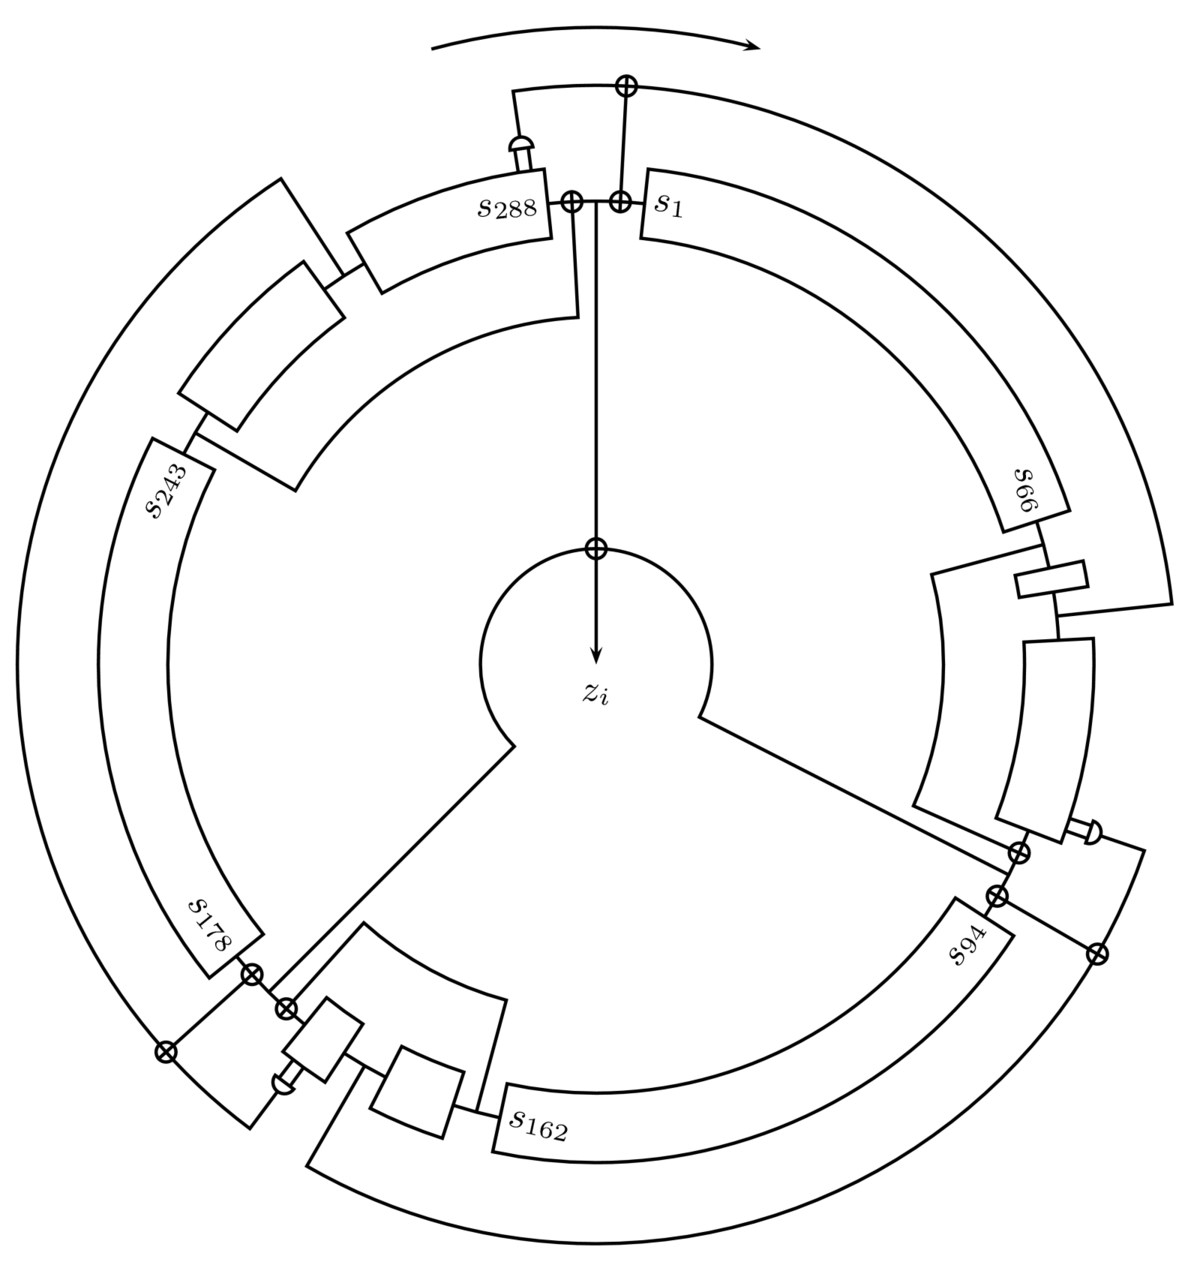
\includegraphics[width=0.5\linewidth]{img/to_harmonize/trivium.png}
    \caption{The trivium stream cipher. Figure extracted from \cite{ISC:DeCanniere06}}.
    \label{fig:triviuml}
\end{figure}


In \cite{DBLP:conf/wahc/BalenboisOS23}, the authors implement Trivium using the original \texttt{tfhe-rs} library, with 2 bits of message and 2 bits of carry for a total of 4 significative bits out of the 32 of a ciphertext component. They call this mode the \texttt{shortint} mode. The use-case they target is transciphering.

To compare our implementation with the one of \cite{DBLP:conf/wahc/BalenboisOS23}, timings are not a good metric as in their work they are provided on a massive AWS instance with a significant amount of parallelism. A better metric is to count the number of PBS and compare the parameter sets.

We reproduced the PBS operation with their parameter set on our machine and then simply estimated the timings of one round of Trivium with their approach with no parallelism. The results are summed up in Table \ref{tab:perfs_trivium}. Note that in our implementation we do not refresh the output bits with a PBS after the chain of \texttt{XOR}, because in the use-case of transciphering one more \texttt{XOR} has to be performed with the message. We take advantage of this and move the last PBS into the transciphering phase.

\begin{table}[htbp]
\centering
\caption{Comparison of timings of one round of Trivium between our work and \cite{DBLP:conf/wahc/BalenboisOS23}, with $\epsilon=2^{-40}$.}
\label{tab:perfs_trivium}
\begin{tabular}{|c|c|c|c|}
\hline
Instance & Timing PBS & Number of PBS per round & Estimated timings \\
\hline
\cite{DBLP:conf/wahc/BalenboisOS23} & 6.6 & 7 & 46.2 ms \\
\hline
Our work & 9.5 & 3 & 28.5 ms \\
\hline
\end{tabular}
\end{table}

\subsection{Keccak Permutation}
\label{sec:keccak}

Keccak is a hash function standardized by NIST under the name \emph{SHA-3} \cite{sha-3}. It is a sponge function, whose transformation is called the \emph{Keccak permutation}. It consists of five sub-functions: $\theta$, $\rho$, $\pi$, $\chi$, and $\iota$.

Let us recall that our approach encrypts each bit in one TFHE ciphertext. Let us explain the stategies of homomorphization of these sub-functions:
\begin{itemize}
    \item $\rho$ and $\pi$ simply reorder the bits within the state, so they are not impacted by the homomorphization.
    \item $\theta$ is just a serie of \texttt{XOR} operations, so it can be performed with a serie of homomorphic additions and without any PBS provided that the input ciphertexts are defined over $\Z_p$ with $p=2$.
    \item $\chi$ is the only non-linear function of the permutation, and has to be performed with a PBS. It is the transformation that applies the function defined by $$f_\chi(a, b, c) = a \oplus c \oplus b \& c$$ to get each bit of the output state.
    \item Finally, $\iota$ performs a simple \texttt{xor} with a constant, so it can be handled in a similar manner that $\theta$. The difference is that the constant is in clear this time.
\end{itemize}
The $p$-encodings we use are:
\begin{itemize}
    \item $\Encoding_{\&} = \EncDef{\{1\}}{\{2\}}$ with $p_\& = 3$  to evaluate the $\&$ operator in the alternative formula of $\chi$.
    \item $\Encoding_\oplus = \EncDefOne{1}$ with $p_\oplus = 2$ for the other operations of $\oplus$.
\end{itemize}
Our strategy of homomorphic evaluation of the Keccak permutation is as follows:
\begin{enumerate}
    \item Encrypt the input state under the encoding $\Encoding_\oplus$.
    \item Evaluate the subfuctions $\theta$, $\rho$, and $\pi$. Theses functions being purely linear, they can be performed only with sums under $\Encoding_\oplus$.
    \item Change the encoding from $\Encoding_\oplus$ to $\Encoding_\&$ with one PBS per bit of the state (Property \ref{prop:enc_switch_pbs}).
    \item Evaluate the \texttt{AND} operator of the subfunction $\chi$ with the gadget \[\Gamma_\& = \left ( (\Encoding_\&, \Encoding_\&), \Encoding_\oplus, 3, 2\right )\] associated to function $f_\& : (x, y) \mapsto x \& y$. This gadget is applied once per bit of the state.
    \item Evaluate the remaining $\oplus$ operators of $\chi$ and the $\iota$ subfunctions, then jump back Step 2. for the next loop iteration.
\end{enumerate}


Casting a ciphertext from $\Encoding_\oplus$ to $\Encoding_\&$ (Step 3) is a bit tricky because $p_\oplus = 2$ is even. Because of the negacyclicity problem, one needs $\Encoding_\&(0) = \modulo{-\Encoding_\&(1)}{p_\&}$. With $p_\& = 3$, the only candidate is the encoding $\Encoding_\&$ defined above.


As a result, each round takes two programmable bootstrappings per bit. An implementation with our tweaked version of \texttt{tfhe-rs} takes 16.5 seconds (without any parallelism) on our hardware to perform one Keccak round on a state of 1600 bits in spite of the two PBS required per round and per bit. Those timings are possible because of the small values of $p$ allowing the use of a set of  small parameters, which speeds up the computation. A full run of Keccak counting 24 rounds, we can then estimate the timings without parallelism to $6.6$ minutes. For the sake of simplicity, we use the same set of parameters for both types of PBS, avoiding the hassle of using two different server keys.


This strategy of implementation complies with the more generic one that we introduce in Section \ref{sec:ascon} and that is illustrated on Figure \ref{fig:layout_spn}. It suits very well the use-cases where linear and non-linear operations are alternating.


\subsection{Ascon}
\label{sec:ascon}


Ascon \cite{JC:DEMS21} is a lightweight block cipher algorithm that was designed to provide efficient and secure encryption and authentication for a wide range of applications, particularly in resource-constrained environments such as embedded systems and IoT devices. The name ``Ascon'' stands for ``Authenticated encryption for Small Constrained Devices''. We implemented its s-box, whose circuit is represented on Figure \ref{fig:ascon}.

\begin{figure}[h]
    \centering
    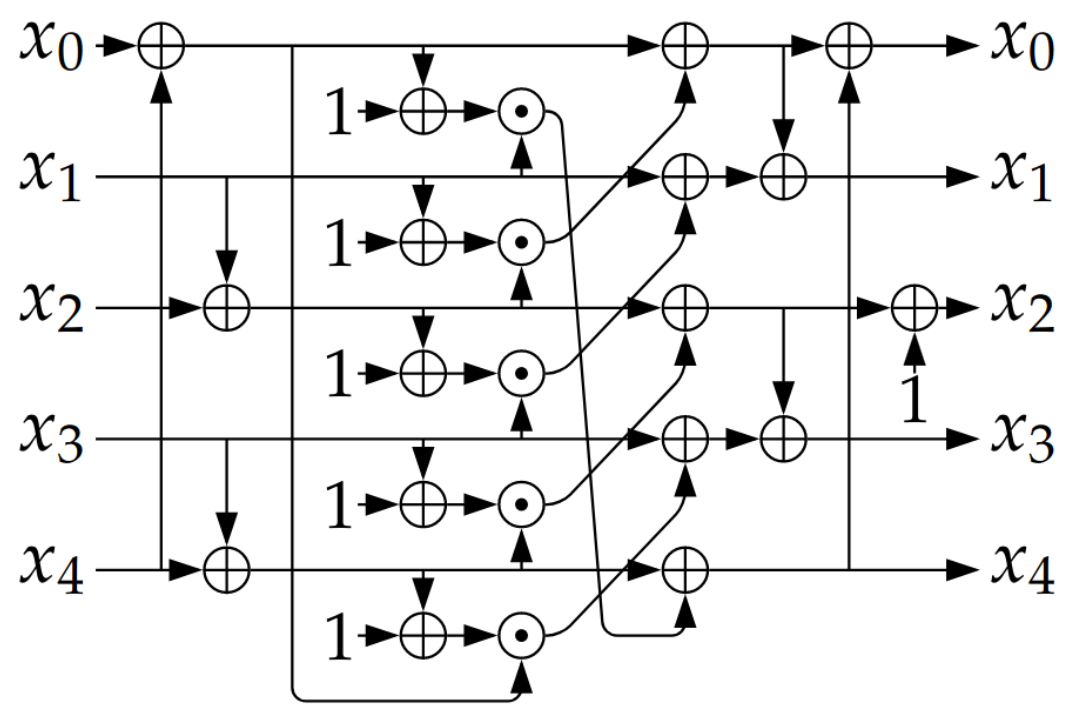
\includegraphics[width=0.5\linewidth]{img/to_harmonize/ascon.png}
    \caption{The 5-bits look-up table of ASCON. Figure extracted from \cite{JC:DEMS21}}
    \label{fig:ascon}
\end{figure}



This layout is a bit different from the others: the s-box takes five bits as input and outputs five bits. We denote $f_0, \dots, f_4$ the five functions of $\B^5 \mapsto \B$ that generate the 5 output bits $x_0, \dots, x_4$. Thus, we need to define five gadgets (one per function).

These functions, once analyzed by the algorithm, can be computed in one single bootstrapping each, but for different values of $p$ (respectively $p=17, 7, 7, 15, 11$ that are the smallest possible values). We could implement the gadgets $\Gamma_0, \dots, \Gamma_4$ (associated to $f_0, \dots, f_4$) with different values for $p_{in}$, but this would imply to introduce some encoding switchings before each round of hashing. To keep things simpler we generated only encodings with $p = 17$, making the implementation more straightforward as no encoding switching is required. For each subfunction $f_i$, five canonical $17$-encodings $(\Encoding_{i, 0}, \dots, \Encoding_{i, 4})$ of form $$\Encoding_{i, j} = \EncDefOne{d_{i,j}}$$ are computed. The results are displayed in the Table \ref{tab:encodings_ascon}. Note the zero values in some cases, they show that the variable is not used in the subfunction. 

The s-box layer is followed by a linear layer, where the bits of the states are shifted and combined with \texttt{XOR} operations. This can be trivially done with $p=2$. Finally, to prepare the next round, an encoding switching is performed to send back the ciphertexts on $17$-encodings. This is summed up in Figure \ref{fig:layout_spn}. Note that there is no encoding switching from non-linear layer to linear layer because the gadgets can directly outputs ciphertexts under $\Encoding_\oplus = \EncDefOne{1}$ with $p=2$.

\begin{figure}
    \centering
    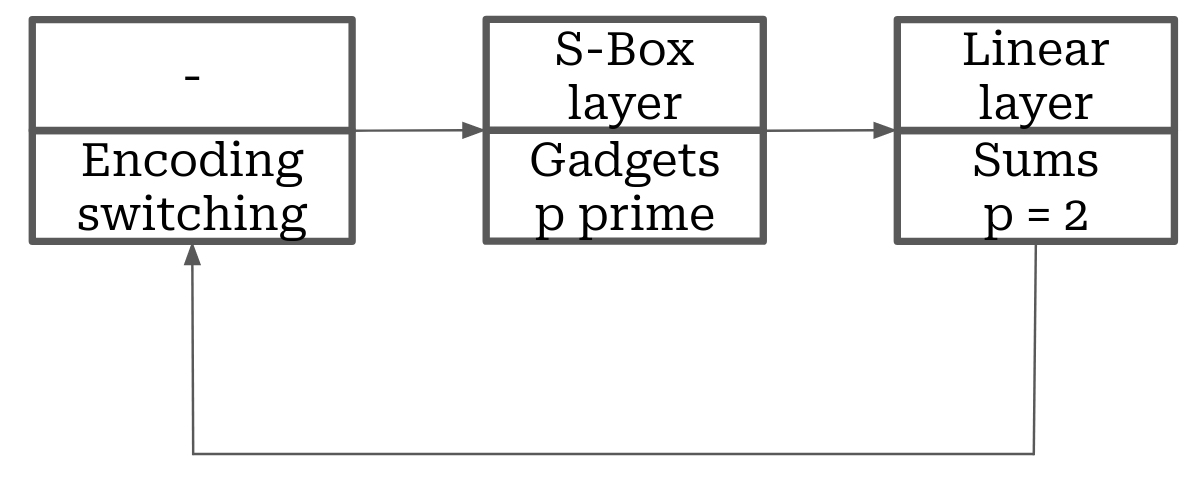
\includegraphics[width=0.5\linewidth]{img/to_harmonize/layout_spn.png}
    \caption{A common layout to evaluate cryptographic primitives. The upper part of the boxes represents what happens in the clear, while the lower part shows the encrypted operations. }
    \label{fig:layout_spn}
\end{figure}


To wrap up, we construct the five gadgets $\Gamma_i = \left ( (\Encoding_{i,0}, \dots,  \Encoding_{i, 4}), \Encoding_\oplus, 17, 2, f_i \right )$. They will carry the evaluation of the s-boxes and output ciphertexts encrypted under $\Encoding_\oplus$. Then, the linear layer is trivially evaluated with homomorphic sums. An encoding switching from $\Encoding_\oplus$ to $\Encoding_{i, j}$ allows to come back to non-linear operations.




\begin{table}[]
    \centering
    \begin{tabular}{|c|c|c|c|c|c|}
        \hline
       subfunction & $d_{i, 0}$ & $d_{i, 1}$ & $d_{i, 2}$ & $d_{i, 3}$ & $d_{i, 4}$\\
        \hline
        $f_0$  & $1$ & $2$ & $3$ & $7$ & $14$\\
        \hline
        $f_1$ & $1$ & $2$ & $2$ & $2$ & $4$\\
        \hline
        $f_2$ & $1$ & $2$ & $2$ & $4$ & $0$\\
        \hline
        $f_3$ & $1$ & $1$ & $5$ & $5$ & $3$\\
        \hline
        $f_4$ & $1$ & $2$ & $0$ & $4$ & $3$\\
        \hline
     \end{tabular}
    \caption{Parameters $d_{i, j}$ for Ascon, with $p=17$ for every subfunction.}
    \label{tab:encodings_ascon}
\end{table}


Using this solution, the s-box is evaluated in $92$ ms. Note that the 5 different PBS described in Table \ref{tab:encodings_ascon} have different norms of vector $\vec d$ so they may have a different set of parameters for each. We use the more restrictive one (i.e. the one with greater $\norm{\nu}$) for the 5. Estimating the timings of a full run of Ascon is not trivial because it depends a lot of the parameters. To give a rough idea, in hashing mode, 64 s-boxes are required per round, with 12 rounds recommended. The outputs of the s-boxes are in $\Z_2$ to allow the evaluation of the linear layer of Ascon. At the end of this linear layer, the encoding of each of the 320 bits of the state must be switched back to $\Z_{17}$ with a PBS. To do so, we use the same set of parameters as for the encoding switching in Step 3 of the Keccak evaluation in Section \ref{sec:keccak}.

This gives an estimation of $89$ seconds for one Ascon hash.


\subsection{AES}
\label{sec:aes}

%\subsubsection{Reminders on AES and Choice of an Alternative Representation}

AES \cite{aes-original}, or Advanced Encryption Standard, stands as one of the most widely used and trusted encryption algorithms in the world of computer security. Its standardization occured in 2001 when it was adopted by NIST to replace the obsolete DES (Data Encryption Standard). Implementing this primitive in FHE is known as particularly tricky and only few attempts have been made \cite{C:GenHalSma12}, \cite{PKC:CorLepTib14}, \cite{trama-aes}.

A round of AES can be decomposed into 4 steps:
\begin{enumerate}
    \item \texttt{SubBytes}: a non-linear substitution step where each byte is replaced by another according to a lookup table. This step concentrates all the challenge for homomorphization, the other one being trivial with our framework.
    \item \texttt{ShiftRows}: a transposition step where the last three rows of the state are shifted cyclically a certain number of times. As our framework encrypts each bit in a distinct ciphertext, this step is for free.
    \item \texttt{MixColumns}: a linear mixing operation which operates on the columns of the state, combining the four bytes in each column. This step can be implemented using only \texttt{XOR} operations and bit-shiftings. The former are trivial with our framework using $p=2$ and the latter are for free as the ones in the previous step.
    \item \texttt{AddRoundKey}: each byte of the state is combined with a byte of the key from the key schedule using a \texttt{XOR}. Still using $p=2$, this can be carried out easily. 
\end{enumerate}


 The s-box of \texttt{SubBytes} takes 8 bits in input and yields 8 bits of output. It is defined by two substeps: an inversion in $GF(2^8)$ followed by an affine transformation. While the latter is trivial to compute with TFHE, the former is much trickier and thus we did not take advantage of this representation. Using our framework, the obvious-looking solution is to split the full s-box $\B^8 \mapsto \B^8$ into 8 subfunctions $f_0, \dots, f_7: \B^8 \mapsto \B$. We could then give them to the search algorithm of Section \ref{sec:search}. If this would work, we could evaluate the Rjindael s-box in 8 PBS. Unfortunately, the algorithm does not converge for values of $p$ ``reasonable'', that is to say less than 7 bits. 


We thus need to leverage an alternative representation of the s-box. A well known efficient Boolean representation of the AES s-box is given in \cite{boyar}. In this work, authors applied logic minimization techniques to produce an optimized Boolean circuit (in terms of number of gates) of the s-box splitted in 3 phases:

\begin{enumerate}
    \item A purely linear layer mapping the 8 input bits onto 22 bits.
    \item A middle non-linear layer, represented by a circuit with exclusively \texttt{AND} and \texttt{XOR} logic gates, mapping the previous 22 bits onto 18 bits.
    \item A final purely linear layer mapping the 18 bits on the 8 output bits of the s-box.
\end{enumerate}


To design our implementation of AES, we will use the strategy we introduced for Keccak (Section \ref{sec:keccak}) and ASCON (Section \ref{sec:ascon}) and that is illustrated on Figure \ref{fig:layout_spn}. The steps \texttt{ShiftRows}, \texttt{MixColumns}, \texttt{AddRoundKeys} only involves \texttt{XOR} operators, so we will carry them out with $p=2$. Same things with the steps 1. and 3. of the circuit of \texttt{SubBytes} of \cite{boyar}. The only part remaining is the Step 2. of the \texttt{SubBytes}, that is a non-linear circuit. We evaluate this circuit using gadgets and the approach introduced in Section \ref{sec:graphs}. A layer of encoding switching allows to link both parts.

 In particular, \texttt{MixColumns} can be reduced to a serie of \texttt{XOR} (in our implementation, we use the circuit designed in \cite{mixcol}). 

In the following, we focus on the implementation of the non-linear layer using the approach by graphs of Section \ref{sec:graphs}.


\subsubsection{Homomorphization of the S-box}


We start from the circuit representation given in the work of \cite{boyar}. This set of instructions is compiled into a circuit $\mathcal{A}$, compliant with the definitions introduced in Section \ref{sec:graph_definition}.


Each of the $18$ outputs $(z_0, \dots, z_{17})$ are isolated from each other and the circuits $(\mathcal{A}_0, \dots, \mathcal{A}_{17})$ generating them are separated. Of course, some intermediary values are used in several circuits, but for now we ignore this and we considerate the $18$ problems as independent from each other. 

Then, for each circuit $\mathcal{A}_i$, we run the algorithm explained in Section \ref{sec:graphs} to produce an efficient graph. We merge all those graphs and run everything for a total of 36 PBS to evaluate the full circuit $\mathcal{A}$, with a global $p = 11$. This allows a relatively quick bootstrapping.

Recall that the \texttt{SubBytes} step is made of 16 s-boxes. So, we can derive that one execution of the \texttt{SubBytes} step takes $16 \times 36 = 576$ PBS. 

The outputs of this step would be encoded with $p=2$, allowing the \texttt{XOR} operations of the following steps to be performed efficiently. We also need to take into account the encoding switching to come back to $p=11$ before each \texttt{SubBytes}. It costs one PBS per bit, so $128$ PBS. Finally, this gives a total of $704$ PBS per round. For \texttt{AES-128}, which takes 10 rounds, we estimate a full run to $7040$ PBS.

\subsubsection{Performances}

In terms of performances, with a set of parameters ensuring a security level of $\lambda=128$ bits and an error probability $\epsilon=2^{-40}$, a PBS takes $17$ ms on our hardware. The total runtime of the whole implementation on one thread is $135$ s. We note that the $16$ evaluations of s-boxes in \texttt{SubBytes} can be parallelized, as well as each of the $128$ encoding switchings before \texttt{SubBytes}. Moreover, within each s-box, we can locally apply our strategy of parallelization introduced in Section \ref{sec:parallelization}.


We compare favorably to previous works of \cite{C:GenHalSma12} and \cite{PKC:CorLepTib14}, who report timings of respectively 18~minutes and 5~minutes for a full AES, Once again, authors do not mention the value of $\epsilon$. The more recent work of \cite{trama-aes}, also proposes an implementation of \texttt{AES-128} using a completely different technique called the \emph{tree-bootstrapping}. On a similar experimental setup, but with a failure probability $\epsilon=2^{-23}$, they claim an execution in $270$~s on one thread. We ran again our code with an other set of parameters tailored for the same $\epsilon$ and obtained a full run in $103$~s.  Note that in our implementation, we used the mode restrictive set of parameters $\texttt{PBS}_{(11, 4)}$ for every bootstrapping (even the ones that should be performed with $\texttt{PBS}_{(2, 1}$. We also derived the theoretical timing that could have been achieved if we had implemented this with two server keys (one for each set of parameters). This theoretical timing should be of $105$ s with $\epsilon=2^{-40}$, we added it in Table \ref{tab:concrete_perfs}.


\subsection{Summary of Applications}
\label{sec:tables_perfs}


We summarize hereafter the parameters and performances of our implementations of cryptographic primitives. Table~\ref{tab:parameters} gives an overview of the TFHE parameters used for each value of $p$ in these examples. They all meet the required level of security of $2^{128}$ and the error probability $\epsilon=2^{-40}$. It also shows the associated $p$ and the norm of $\vec d$, denoted by $\mathcal{N}_{\vec d}$ (that corresponds to $\mathcal{N}_{\vec d} = \lceil \log_2(\customnorm{\vec d}) \rceil$) that are the input of the parameter selection algorithm. To allow the comparison with the strategy of gate bootstrapping, we also included the set of parameters hardcoded in \texttt{tfhe-rs} to evaluate boolean operators. Table \ref{tab:complexity_primitives} shows the complexity of the cryptographic primitives expressed in PBS with our framework. It can be compared with Table \ref{tab:gates}, that illustrates the number of PBS required with the naive strategy of gate bootstrapping. Finally, Table \ref{tab:concrete_perfs} shows the concrete performance achieved by our implementations on our machine, as well as the comparison with other works and with the gate bootstrapping. For more information about an implementation or a comparison, the reader is referred to the related section.

\newcommand{\PBS}{\mathsf{PBS}}

\begin{table}
    \centering
    \small % Adjust font size if necessary
    \begin{tabular}{|l|c||c|c|c|c|c|c|c|c|c||c|}
            \hline
        \multicolumn{2}{|c||}{\textbf{Identification}} & \multicolumn{9}{c||}{\textbf{TFHE parameters}} & \textbf{Timings} \\
        \hline
        Ref. & Sections & $n$ & $k$ & $N$ & $\sigma_{\texttt{\LWE}}$ & $\sigma_{\texttt{\GLWE}}$ & $B_g$ & $\ell_g$ & $B_{KS}$ & $\ell_{KS}$ & PBS\\
        \hline
        \hline
            \texttt{$\PBS_{gate}$} & Table \ref{tab:gates} & 722 & 2 & 512 & $2^{16.2}$ & $2^{7.8}$ & $2^6$ & 3 & $2^3$ & 4 & 10 ms\\
           \hline
          \hline
        \texttt{$\PBS_{(9, 2)}$} & \ref{sec:simon}, \ref{sec:trivium} & 684 & 3 & 512 & $2^{16}$ & $2^{2}$& $2^{10}$ & 2 & $2^3$ & 4 & 9.5 ms\\
           \hline
       
        \texttt{$\PBS_{(3, 2)}$} & \ref{sec:keccak} & 676 & 5 & 256 & $2^{22}$ & $2^{7}$& $2^{18}$ & 1 & $2^4$ & 3 & 5.25 ms \\
          \hline
    
        \texttt{$\PBS_{(2, 1)}$} & \ref{sec:keccak}, \ref{sec:ascon} & 676 & 5 & 256 & $2^{22}$ & $2^{7}$& $2^{18}$ & 1 & $2^4$ & 3 & 5.25 ms \\
         \hline
        
        \texttt{$\PBS_{(17, 5)}$} & \ref{sec:ascon} & 740 & 2 & 1024 & $2^{13}$ & $2^{2}$& $2^7$ & 3 & $2^5$ & 3 & 18 ms\\
         \hline
        
        \texttt{$\PBS_{(11, 4)}$} & \ref{sec:aes} & 708 & 3 & 512 & $2^{15}$ & $2^{2}$& $2^6$ & 4 & $2^2$ & 7 & 17 ms  \\
            \hline
       \end{tabular}

    \medskip 
    
    \caption{Sets of TFHE parameters for each PBS used in our implementations, with the constraints used to generate the sets, and the performances. Each setting is referenced as \texttt{$\PBS_{(p, \mathcal{N}_d)}$} with $\mathcal{N}_d = \lceil \log_2(\customnorm{d})\rceil$. All this parameters ensure a level of security $\lambda=128$ bits and a failure probability of bootstrapping of $\epsilon=2^{-40}$. $q$ is always fixed to $2^{32}$. \texttt{$\PBS_{gate}$} refers to the naive case of the gate bootstrapping implemented in \cite{tfhe-rs} and is used to estimate the timings of the naive strategy in Table \ref{tab:concrete_perfs}.}
    \label{tab:parameters}
\end{table}



\begin{table}
    \centering
    \begin{tabular}{|c|c|c|}
        \hline
        \textbf{Section} & \textbf{Primitive} & \textbf{Complexity in PBS}  \\
        \hline
        \multirow{2}{*}{\ref{sec:simon}} & One round of SIMON-128 & 64 \texttt{$\PBS_{(9, 2)}$}\\
        \cline{2-3}
        & One full run of SIMON-128 & 4352 \texttt{$\PBS_{(9, 2)}$}\\
        \hline
        \multirow{2}{*}{\ref{sec:trivium}} & One round of Trivium & 3 \texttt{$\PBS_{(9, 2)}$}\\
        \cline{2-3}
        & ~One warm-up phase of Trivium $(*)$~ & 3456 \texttt{$\PBS_{(9, 2)}$}\\
        \hline
        \multirow{2}{*}{\ref{sec:keccak}} & One round of Keccak & 1600 \texttt{$\PBS_{(3, 2)}$} $+$ 1600 \texttt{$\PBS_{(2, 1)}$}\\
        \cline{2-3}
        & A full Keccak permutation $(*)$ & ~38400 \texttt{$\PBS_{(3, 2)}$} $+$ 38400 \texttt{$\PBS_{(2, 1)}$} ~\\
        \hline
      \multirow{2}{*}{ \ref{sec:ascon}} & One evaluation of Ascon's s-box & 5 \texttt{$\PBS_{(17, 5)}$}\\
      \cline{2-3}
      & One full Ascon hashing run $(*)$ & 3840 \texttt{$\PBS_{(17, 5)} + 3840 \PBS_{(2, 1)}$}\\
        \hline
        \multirow{2}{*}{\ref{sec:aes}} & One evaluation of the AES s-box & 36 \texttt{$\PBS_{(11, 4)}$}\\
        \cline{2-3}
        & A full run of \texttt{AES-128}  & 5760 \texttt{$\PBS_{(11, 4)}$} + 1280 \texttt{$\PBS_{(2, 1)}$}\\
        \hline
    \end{tabular}
    \medskip
    \caption{Complexity of the different primitives we implemented with respect to the PBS of Table~\ref{tab:parameters}. The primitives indicated by a $(*)$ are estimations while the others have been fully implemented.}
    \label{tab:complexity_primitives}
\end{table}



\begin{table}
    \centering
    \begin{tabular}{|c|c|c|}
        \hline
        \textbf{Section} & \textbf{Primitive} & \textbf{Number of logic gates}  \\
        \hline
        \multirow{2}{*}{\ref{sec:simon}} & One round of SIMON-128 & 256\\
        \cline{2-3}
        & One full run of SIMON-128 & 17408\\
        \hline
        \multirow{2}{*}{\ref{sec:trivium}} & One round of Trivium & 13\\
        \cline{2-3}
        & ~One warm-up phase of Trivium $(*)$~ & 14976\\
        \hline
        \multirow{2}{*}{\ref{sec:keccak}} & One round of Keccak & 7687\\
        \cline{2-3}
        & A full Keccak permutation $(*)$ & 184488\\
        \hline
      \multirow{2}{*}{ \ref{sec:ascon}} & One evaluation of Ascon's s-box & 16\\
      \cline{2-3}
      & One full Ascon hashing run $(*)$ & 19968\\
        \hline
        \multirow{2}{*}{\ref{sec:aes}} & One evaluation of the AES s-box & 115 (\cite{boyar})\\
        \cline{2-3}
        & A full run of \texttt{AES-128}  & 23360 (\cite{boyar}, \cite{mixcol})\\
        \hline
    \end{tabular}
    \medskip
    \caption{Number of logic gates in the circuit of each primitive. This shows the heavy cost of the naive method of performing one bootstrapping per gate (except the \texttt{NOT} ones).}
    \label{tab:gates}
\end{table}


\begin{table}
    \centering
    \scalebox{0.9}{
    \begin{tabular}{|c|c|c|}
    \hline
       \textbf{Primitive} & \textbf{Section or Other work} & \textbf{Performances} \\
    \hline
    \hline
        \multirow{3}{*}{One full run of SIMON} & Gate Bootstrapping & 174 s\\
        \cline{2-3}
        & \cite{cryptoeprint:2023/480} $\dagger$ & 128 s\\
        \cline{2-3}
         & Our work (Section \ref{sec:simon}) & 10 s \\
         \hline
         \hline
         \multirow{3}{*}{One warm-up phase of Trivium (*)} & Gate Bootstrapping & 1498 s\\
         \cline{2-3}
         & ~\cite{DBLP:conf/wahc/BalenboisOS23} (estimation on our machine)~ & 53 s\\
        \cline{2-3}
         & Our work (Section \ref{sec:trivium}) & 32.8 s\\
         \hline
         \hline
        \multirow{2}{*}{One Full Keccak permutation $(*)$} & Gate Bootstrapping & 30.7 min\\
        \cline{2-3}
        & Our work (Section \ref{sec:keccak}) & 8.8 min\\
        \hline
        \hline
        \multirow{2}{*}{One Ascon hashing $(*)$} & Gate Bootstrapping & 200s \\
        \cline{2-3}
        & Our work (Section \ref{sec:ascon}) & 92 s \\
        \hline
        \hline
        \multirow{4}{*}{\begin{tabular}{c}
            One full evaluation of AES-128   \\
            ($\epsilon=2^{-23}$) on one thread \\
        \end{tabular}} & \cite{C:GenHalSma12} $\dagger$ & 18 min\\
        \cline{2-3}
        & \cite{PKC:CorLepTib14} $\dagger$ & 5 min\\
        \cline{2-3}
        & \cite{trama-aes} & 270 s\\
        \cline{2-3}
        & Our work (Section \ref{sec:aes}) & 103 s\\
    \hline
        \multirow{3}{*}{\begin{tabular}{c}
            One full evaluation of AES-128   \\
            ($\epsilon=2^{-40}$) on one thread \\
        \end{tabular}} & Gate Bootstrapping & 234 s \\
        \cline{2-3}
        & Our work (Real implementation) & 135 s\\
        \cline{2-3}
        & Our work (Theoretical timing with two keys) & 105 s\\
    \hline
    \end{tabular}}
    
    \medskip 
    
    \caption{Timings of evaluation of full primitives, and comparison with previous works when they exist. Like on Table \ref{tab:complexity_primitives}, a star $(*)$ is added in the cells if our timing is not obtained from a full implementation but estimated from an implemented building block. Also, the security level of each implementation is $\lambda=128$ and the default error probability is $\epsilon=2^{-40}$. The concurrent works that do not indicates their $\epsilon$ are marked with $\dagger$. }
    \label{tab:concrete_perfs}
\end{table}

\section{Conclusion}

In this chapter, we presented a first application of our technique of using an odd plaintext modulus: by embedding $\ell$ bits into a prime field, it becomes possible to unlock the full potential of homomorphic addition and ``pack'' several bits into a ciphertext. We can then retrieve the result of any Boolean function $f:\B^\ell \mapsto \B$ by a unique bootstrapping. This approach scales much better than the conventional technique of using a \gls{LUT} of size $2^\ell$.

We ended this chapter by presenting an homomorphic implementation of the \gls{AES} scheme. Implementing the circuit of the S-box using our technique was by far the most challenging part of this design. This is not very surprising: this component has been designed to prevent cryptanalysis,  which indirectly makes the circuit representation of this function unsuitable for this kind of Boolean-oriented approaches.

An interesting axis of improvement would be to use an \textit{arithmetic} representation of the values, so the S-box would simply be evaluated as a \gls{LUT}. But by fully committing to arithmetic representation, the linear part of the scheme (so the \ShiftRows, \MixColumns and \AddRoundKey steps) becomes the new bottleneck, as we could not leverage the additive homomorphism of \gls{TFHE} to evaluate XOR operations anymore. In the next chapter, we elaborate further on these ideas and construct a more efficient version of homomorphic \gls{AES} by combining both Boolean and arithmetic representations. 





\chapter{Accelerating Homomorphic AES Evaluation}
\label{chap:hyppogriph}
% !TeX_ROOT=../../thesis.tex

%\documentclass[version=final]{iacrcc}
%\usepackage[T1]{fontenc}
%\usepackage{graphicx}
%\usepackage{amssymb}
%\usepackage{amsmath}
%\usepackage{amsthm}
%\usepackage{stmaryrd}
%\usepackage{algorithm, float}
%\usepackage[noend]{algpseudocode}
%\usepackage{array}
%\usepackage{tabularx}
%\usepackage{xcolor}
%\usepackage{bbold}
%\usepackage{subcaption}
%\usepackage{xfrac}
%\usepackage{listings}
%\usepackage{fancyvrb}
%\usepackage{comment}
%\usepackage{algpseudocode}
%\usepackage{algorithm}
%\usepackage{longtable}
%\usepackage{adjustbox}
%\usepackage{lmodern}
%\usepackage{MnSymbol,wasysym}
%\usepackage{enumitem}
%\usepackage{listings}
%\usepackage{tcolorbox}
%%%\usepackage[font=small,skip=0pt]{caption}
%\usepackage{amsthm} % For the environment "primitive"
%\usepackage{pgf,tikz}
%\usepackage{xcolor}
%\usepackage{multirow}
%\usepackage[normalem]{ulem}
%


%
%\begin{abstract}
% Making the most of TFHE advanced capabilities such as programmable or circuit bootstrapping and their generalizations for manipulating data larger than the native plaintext domain of the scheme is a very active line of research. In this context, AES is a particularly interesting benchmark, as an example of a nontrivial algorithm which has eluded ``practical'' FHE execution performances for years, as well as the fact that it will most likely be selected by NIST as a flagship reference in its upcoming call on threshold (homomorphic) cryptography. Since 2023, the algorithm has thus been the subject of a renewed attention from the FHE community and has served as a playground to test advanced operators following the LUT-based, $p$-encodings or several variants of circuit bootstrapping, each time leading to further timing improvements. Still, AES is also interesting as a benchmark because of the tension between boolean- and byte-oriented operations within the algorithm. In this paper, we resolve this tension by proposing a new approach, coined ``\hippo'', which consistently combines the (byte-oriented) LUT-based approach with a generalization of the (boolean-oriented) $p$-encodings one to get the best of both worlds. In doing so, we obtain the best timings so far, getting a \emph{single-core} execution of the algorithm over TFHE from $46$ down to $32$ seconds and approaching the $1$ second barrier with only a mild amount of parallelism. We should also stress that all the timings reported in this paper are consistently obtained on the same machine which is often not the case in previous studies. Lastly, we emphasize that the techniques we develop are applicable beyond just AES since the boolean-byte tension is a recurrent issue when running algorithms over TFHE.
%\end{abstract}
%



The last example of application of the previous chapter was to evaluate homomorphically the AES cipher.  But why would one want to perform such a computation in the first place?

There are two answers to this question. First,  AES is a particularly interesting benchmark, as an example of a nontrivial algorithm which has eluded ``practical'' FHE execution performances for years. This is part of the reason why it will most likely be selected by NIST as a flagship reference in its upcoming call on threshold (homomorphic) cryptography \cite{call_nist}. Since 2023, the algorithm has thus been the subject of a renewed attention from the FHE community and has served as a playground to test advanced operators\cite{DBLP:conf/wahc/TramaCBS23, ISC:WWLLL23, TCHES:BonPoiRiv24, TCHES:WLWLLW24}. AES is particularly interesting as a benchmark notably because of the tension between boolean- and byte-oriented operations within the algorithm.


There is also a more down-to-earth reason: evaluating symmetric ciphers using FHE is the core of a cryptographic technique called \textit{transciphering}, which is a promising solution for solving the \textit{ciphertext expansion} problem of FHE. In this protocol, the client first encrypts its data using a symmetric encryption scheme and sends both the encrypted data and (once and for all) the FHE-encrypted symmetric key to the server. Leveraging its encrypted-domain computing capabilities, the server can then decrypt the encrypted data \emph{within the homomorphic domain}, ultimately producing homomorphic ciphertexts on which it can perform the requested calculations. With this trick, the amount of data uploaded by the client is drastically reduces, as symmetric ciphertexts are much lighter than homomorphic ones.


In this chapter, we introduce \hippo, the fastest homomorphic implementation of AES using TFHE at the time of writing. To construct it, we leveraged three main ideas:

\begin{itemize}
	\item[-] We generalized the $p$-encoding construction introduced in Chapter \ref{chap:p_encodings} to the arithmetic case.
	\item[-] The LUT-oriented implementation of \cite{DBLP:conf/wahc/TramaCBS23} is very efficient to evaluate the large Sbox of AES, so we borrowed this idea as it was.
	\item[-] We associated both previous techniques by developing a framework of conversion between Boolean and arithmetic representations.
\end{itemize}


The result of this work is doubly interesting: first, we manage to outperform the rest of the literature on homomorphic AES evaluation. Second, we develop a generic framework useful to resolve the recurring tension between Boolean and arithmetic representations within homomorphic circuits, which we believe is of independent interest.


We start this chapter by introducing the notion of transciphering in Section \ref{sec:transciphering}, which will be a recurring theme in the rest of this manuscript. Then, after some preliminaries on the AES cipher (Section \ref{sec:preliminaries_aes}), we introduce in Section \ref{sec:previous-blocks} some advanced homomorphic operators from \cite{DBLP:conf/wahc/TramaCBS23} that will be useful in this work. We then generalize the $p$-encoding construction of Chapter \ref{chap:p_encodings} to the arithmetic case (Section \ref{sec:generalization_p_encodings}). Finally, Section~\ref{sec:hippogryph_our_work} introduces our new design and Section~\ref{sec:comparison} presents a detailed comparison with existing approaches, supported by relevant benchmarks.


\TODO{Mettre la table récapitulative du papier ici ?}



\section{Introduction to Transciphering}
\label{sec:transciphering}


One common challenge with all FHE schemes is that the ciphertexts are much larger than the corresponding plaintexts. 
For example, a plaintext message of a few kilobytes can require tens or even hundreds of megabytes of data, making the processing of large data sets impractical. While compression techniques can help reduce the expansion factor in TFHE ciphertexts, the encrypted data still remains an order or two of magnitude larger than the original plaintext. 

It is possible to mitigate this issue using \emph{transciphering}~\cite{transciphering}. The idea is to off-load the task of actually encrypting the data to a symmetric cipher, and to simply encrypt homomorphically the key that is used. The user then sends both the homomorphically encrypted key and the ciphertext to the server, which can then homomorphically decrypt the received ciphertexts. This is done by running a fully homomorphic evaluation of the decryption function of the symmetric cipher, producing valid homomorphic ciphertexts representing the data. The server can then proceed to the homomorphic operations, like in the traditional FHE setting. This principle is illustrated on Figure \ref{fig:transciphering}

\begin{figure}
	\centering
	
	\begin{tikzpicture}

		%%%% Client Side (with its keys)%%%%%%%%%
		
		%%%Header%%%%%%%%%%%%%
		\node (client) at (0,0) {
			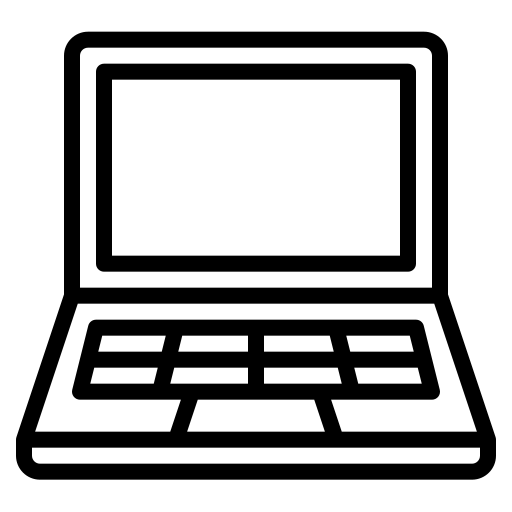
\includegraphics[width=\sizenode cm]{img/blocks_from_slides/assets/laptop.png} % Replace with your image file
		};
		\node at ($(client) + (0, 1)$) {Client};
		
		\node (fhe_key_client) at ($(client.east) + (0.1, -0.5)$) {
			
\includegraphics[width=\sizeindice cm]{img/blocks_from_slides/assets/green_key.png}
		};
		
		\node (sym_key_client) at ($(fhe_key_client.east) + (0.2, 0)$) {
			
\includegraphics[width=\sizeindice cm]{img/blocks_from_slides/assets/red_key.png}
		};
		%%%%%%%%%%%%%%%%%%%%%%%
	
	
	
		%%%%%%%%%%%%%%%Chiffrement symétrique%%%%%%%%%%%%%
		
		% node enc_sym
		\encsym{$(client.south) + (0, -1)$}
	
		\node (clear data) at ($(enc_sym.west) +  (-1, 0)$) { 
			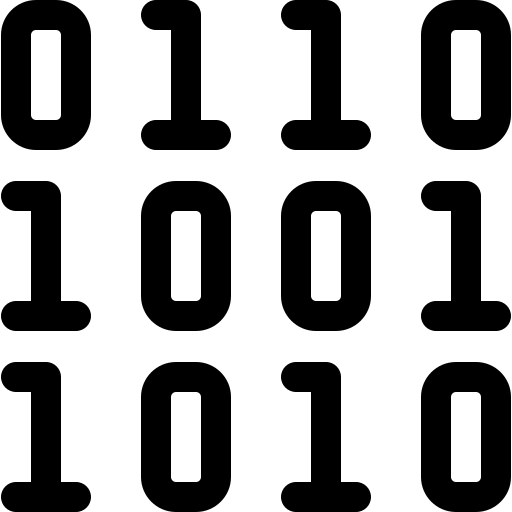
\includegraphics[width=\sizenode cm]{img/blocks_from_slides/assets/data.png} % Replace with your image file
		};
	
		\encrypteddata{$(enc_sym.east) + (1, 0)$}
		\draw[-latex] (clear data) -- (enc_sym);
		\draw[-latex] (enc_sym) -- (data_sym);
		
		\node (one) at ($(clear data) - (1, 0)$) {1.};
		
		%%%%%%%%%%%%%%%%%%%
		
		
		%%%%%%%%% Chiffrement homomorphe de la clé%%%%%%%%%%%%
	
		\encfhe{$(enc_sym) + (0, -2)$}
		\node (fhe_key) at ($(enc_fhe.west) + (-1, 0)$) { 
				
\includegraphics[width=\sizenode cm]{img/blocks_from_slides/assets/red_key.png} % Replace with your image file
			};
		
		\encryptedkey{$(enc_fhe.east) + (1, 0)$}
	
		\draw[-latex] (fhe_key) -- (enc_fhe); 
		\draw[-latex] (enc_fhe) -- (encrypted_key);
			
		\node (two) at ($(fhe_key) - (1, 0)$) {2.};
		%%%%%Server Side %%%%%%%

		\node (server) at (8,0) {
			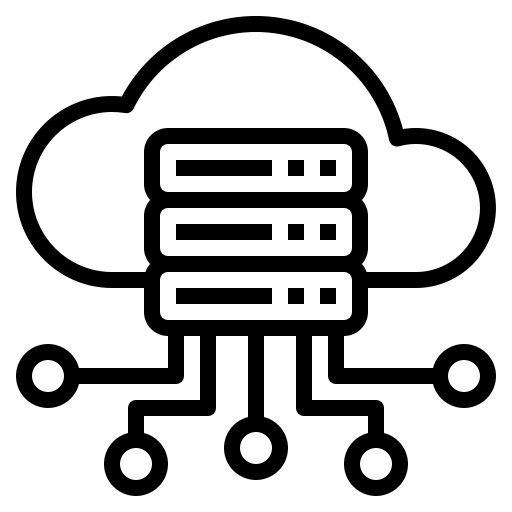
\includegraphics[width=\sizenode cm]{img/blocks_from_slides/assets/server.png} % 
		};
		
		\node at ($(server) + (0, 1)$) {Server};
		
		%%%%%Evaluation Key%%%%%
		
		\node (evaluation_key_server) at ($(server.east) + (0.1, -0.5)$) {
			
\includegraphics[width=\sizeindice cm]{img/blocks_from_slides/assets/evaluation_key.png}
		}; 
		
		%%%%%%%%%%Transfert de la donnée chiffrée et de la clé
		
		
		\encrypteddata{$ (enc_fhe.south) +(3, -2)$}
		\encryptedkey{$ (enc_fhe.south) +(5, -2)$}
		
		\draw[color=gray, thick, opacity=0.6, dash pattern=on 6pt off 3pt] ($(data_sym) - (1, 1)$) rectangle ++(4,2);
		
		\draw[->, gray, >=stealth, line width=1mm, opacity=0.6] ($(data_sym) - (1.5, 1.5)$) -- ++(5,0);
		
		\node (three) at ($(data_sym) - (1.5, 0)$) {3.};
		
		
		%%%%%Déchiffrement homomorphe de la donnée%%%%%%
			
		\transciphering{$(server.south) + (0, -9)$}
		
		\encrypteddata{$(transciphering.west) + (-1, 0)$}
		
		\encryptedkey{$(transciphering.south) + (0, -1)$}
		
		\fhedata{$(transciphering.east) + (1, 0)$}
		
		\draw[-latex] (data_sym) -- (transciphering);
		\draw[-latex] (encrypted_key) -- (transciphering);
		\draw[-latex] (transciphering) -- (data_fhe)    ; 
			
		\node (four) at ($(data_sym) - (1, 0)$) {4.};        
        %%%%%%%%%% Etape 5: evaluation du réseau de neurone homomorphe
        
        \fheneuralnetwork{$(encrypted_key) + (0, -2)$}
        
        \fhedata{$(fhe_neural_network.west) - (1, 0)$}
	
        \fheresult{$(fhe_neural_network.east) + (1, 0)$}
% 
        \draw[-latex] (data_fhe) -- (fhe_neural_network); 
        \draw[-latex] (fhe_neural_network) -- (result_fhe);
%        
        \node (five) at ($(data_fhe) - (1, 0)$) {5.};
        
        %%%%%%%%%Sep%%%%%%%
        \draw (4, 0) -- (4, -14);
                
	\end{tikzpicture}
	

	\captionsetup{singlelinecheck=off}
	\caption[]{An illustration of the transciphering process: \\
		\begin{enumerate}
			\item Data is encrypted with the symmetric cipher.
			\item The symmetric key is homomorphically encrypted.
			\item The client uploads both the encrypted data, as well as the encrypted key.
			\item The server homomorphically evaluates the decryption algorithm of the symmetric cipher, using the symmetric key homomorphically encrypted. It retrieves the data, as valid homomorphic ciphertexts.
			\item The server can then evaluate the homomorphic application!
		\end{enumerate}
		The red color is for symmetric algorithms, green for FHE, and hatched algorithms means that they are evaluated homoomorphically.
	}
	\label{fig:transciphering}
\end{figure}



Implementing FHE encryption through transciphering solves the bandwidth issue: the data sent by the client to the server is encrypted using a symmetric cipher, thus avoiding the significant ciphertext 
expansion implied by direct FHE encryption. The only exception is the symmetric key, which does experience expansion, but this overhead is amortized across the entire data set.

But still, a question remains: which symmetric cipher should we use ? The straightforward solution is to simply pick something very standard, such as AES, and turn it into a homomorphic version. This is what the first works on transciphering tried to do: the first attempt to transcipher AES ciphertexts into FHE data was made in 2012 by Gentry, Halevi, and Smart \cite{C:GenHalSma12}. They used the BGV scheme~\cite{ITCS:BraGenVai12}, a fully homomorphic encryption method based on the Ring-LWE problem, as implemented in HElib~\cite{EPRINT:HalSho20}, an open-source library for FHE. However, their implementation resulted in an execution latency of 17.5 minutes, with now obsolete parameters (despite an amortized cost of 5.8 seconds per block).

Since then, some progress have been made. We give a tour of the current litterature on the topic in Section \ref{sec:comparison}. But still, it seems that fast data transmission with AES will remain impractical, because its design is not adapted at all to homomorphic evaluation.


That is why many researchers have since developed new ``FHE-friendly'' symmetric cryptosystems to improve efficiency. Several proposal exists, including block ciphers such as LowMC \cite{EC:ARSTZ15}, PRINCE \cite{AC:BCGKKK12}, and CHAGHRI \cite{CCS:AshMahTop22}, as well as stream ciphers like Elisabeth \cite{AC:CHMS22}, PASTA \cite{TCHES:DGHRSW23}, Kreyvium \cite{FSE:CCFLNP16} and Transistor \cite{EPRINT:BBBBCL25}. These new schemes, sometimes referred to as hybrid encryption schemes, offer faster and more efficient homomorphic execution, though none have yet been standardized.


Still, homomorphic AES remains an active line of research in the FHE community. In 2022, the National Institute of Standards and Technology (NIST) announced a future call for threshold encryption with a specific focus on FHE, indicating that AES would serve as the benchmark for evaluating proposals \cite{call_nist}. It particularly exemplifies the challenge of switching between boolean- and byte-oriented operations, a recurrent issue in TFHE-based implementations.




 % !TeX_ROOT=../../thesis.tex
 
\section{Preliminaries on AES}
\label{sec:preliminaries_aes}

The Advanced Encryption Standard (AES), based on the Rijndael algorithm winner of the NIST competition in 2000 \cite{aes-original}, is a symmetric block cipher supporting key sizes of 128, 192, and 256 bits. Depending on the key size, AES uses 10, 12, or 14 rounds of processing, each applying a fixed sequence of substitution, permutation, and mixing steps to transform plaintext into ciphertext (or ciphertext into plaintext for decryption). A key schedule generates round keys for each encryption round, plus an initial key.

\hippo focuses on AES with 128-bit keys, which uses 10 rounds. The encryption begins with an \AddRoundKey step, followed by 10 rounds. Each round includes four steps: \SubBytes, \ShiftRows, \MixColumns, and \AddRoundKey, except the final round, which omits \MixColumns. Below, we recall the key expansion and the subroutines:
\begin{itemize}
\item \texttt{Key Expansion}: The \texttt{Key Expansion} operation is performed once for a given secret key. Starting from the 128-bit key (in our context), it generates eleven 128-bit round keys, which are then used in the \AddRoundKey operation throughout the AES encryption or decryption process, without needing access to the original key. The key expansion involves XORs and $\F_{256}$ multiplications.

    \item \SubBytes: The \SubBytes operation is the only non-linear transformation in the cipher. It involves a substitution step, where each byte in the state matrix is replaced according to a fixed S-box. Since it operates independently on each byte of the state, \SubBytes can be easily parallelized, allowing for more efficient execution.
    \item \AddRoundKey: 
    %Before encryption begins, the secret key undergoes an "expansion" process to generate several round keys. The encryption procedure relies solely on these round keys, rather than the initial secret key. 
    During this transformation, the state is updated by combining it with the current round key using a bitwise XOR operation. Specifically, the 128-bit round key is organized into a matrix format to align with the structure of the state matrix, and the two matrices are XORed element-wise to produce the new state.
   
    \item \ShiftRows: The \ShiftRows step is a byte transposition that cyclically shifts the rows of the state by different offsets. For AES with 128-bit keys, the first row remains unchanged, the second row is shifted by one byte, the third by two bytes, and the fourth row by three bytes. 

    \item \MixColumns: The \MixColumns step processes the state column by column through matrix multiplication. To compute each byte of the state matrix, they combine scalar multiplication in $\mathtt{GF}(256)$ with XOR operations. This approach facilitates parallelization of the operation.  
    
    
\end{itemize}




\section{Some Building Blocks for LUT-based Evaluation}
\label{sec:previous-blocks}


In this section, we present the approach from \cite{DBLP:conf/wahc/TramaCBS23}, some components of which we use for our own work. We formally present some advanced homomorphic primitives used in this work that we reuse as well.


\cite{DBLP:conf/wahc/TramaCBS23} is a ``Full-LUT'' approach, that is to say AES is evaluated entirely with TFHE's programmable bootstrapping, encoding exclusively all operations within LUTs. To meet the performance constraints of the bootstrapping algorithm, this method operates on elements in $\Z_{16}$, ensuring efficient computation.

\subsection{AES Subroutines as LUTs}

The \SubBytes step, which involves the evaluation of an S-box, is inherently a LUT operation and is therefore naturally implemented in FHE using a PBS. However, PBS is too slow in $\F_{256}$ (as we have seen in Section \ref{sec:pbs_performances}). So, they rely on a construction evaluating PBS over $\Z_{16}$ rather than $\F_{256}$. Moreover, converting the other AES steps into LUT evaluations also requires additional effort.

In particular, in the original AES design \cite{aes-original}, the \MixColumns step is computed using a series of XOR operations and multiplications in $\F_{256}$. Unfortunately, TFHE’s native multiplication \texttt{ClearMultTFHE} cannot directly handle these $\F_{256}$ multiplications because of the polynomial nature of the elements of this field. As a result, \MixColumns must be reformulated as a LUT evaluation.

Additionally, the \AddRoundKey step, which uses XOR as its key operation, presents its own challenges because XOR is a bivariate operation that requires two inputs. Classical bootstrapping, which operates on single inputs, is insufficient for this purpose. To address this, the authors utilize a specialized bootstrapping method that supports operations on multiple encrypted inputs.

\subsection{LUTs Evaluation} 
Since the AES evaluation involves computing an 8-bit S-box, a straightforward solution would be to work with 8-bit messages. With such messages, the homomorphic S-box evaluation would require only one bootstrapping per byte. However, processing messages with more bits significantly slow down the bootstrapping process. To address this issue, \cite{DBLP:conf/wahc/TramaCBS23} proposes a decomposition approach and demonstrates that the optimal representation of 8-bit inputs for their purpose is in $\Z_{16}$. Specifically, a message $m \in \{0, \cdots, 255\}$ is split into two 4-bit chunks (or \emph{nibbles}) $h$ and $l$ such that $m = 16h+l$. The encryption of $m$ is then represented as two ciphertexts encrypting $h$ and $l$ with the same key $\lweSecretKey$.

However, bootstrapping these decomposed inputs requires a method capable of handling multiple encrypted inputs. The authors explore several approaches for this, namely the chain-based method and the tree-based method \cite{TCHES:GuiBorAra21}. Their analysis concludes that the Tree-Based Method (TBM) is the most suitable for their needs. They also relies on the Multi-Value Bootstrapping (MVB) to produce several outputs for the cost of one PBS. We provide details about TBM and MVB in the following:

\paragraph{Multi-Value Bootstrapping from \cite{RSA:CarIzaMol19}.}
\label{primitive:mvb}
%
Multi-Value Bootstrapping (MVB) is a technique that enables the evaluation of $k$ distinct Look-Up Tables $(f_i)_{1 \le i \le k}$ on a single encrypted input, using only one $\BlindRotate$. This method is based on the factorization of the accumulator polynomials $\textsf{acc}_i(X)$ associated with each function $f_i$. Specifically, each accumulator polynomial is expressed as: 
$$
    \textsf{acc}_i(X) = \sum_{j=0}^{N-1} \alpha_{i,j} X^j, \quad \alpha_{i,j} \in \mathbb{Z}_q.
$$
The factorization then splits it into two parts: 
$$
    \textsf{acc}_i(X) = v_0(X) \cdot v_i(X) \mod (X^N + 1),
$$
where $v_0(X)$ is a common factor shared across all accumulators set as:
$$
    v_0(X) = \frac{1}{2} \cdot (1 + X + \dots + X^{N-1}),
$$
and $v_i(X)$ is a distinct factor specific to each function $f_i$:
$$
    v_i(X) = \alpha_{i, 0} + \alpha_{i, N-1} + (\alpha_{i, 1} - \alpha_{i, 0}) \cdot X + \dots + (\alpha_{i, N-1} - \alpha_{i, N-2}) \cdot X^{N-1}.
$$
This factorization is made possible thanks to the identity:
$$
(1 + X + \dots + X^{N-1}) \cdot (1-X) \equiv 2 \mod (X^N + 1).
$$
By leveraging this factorization and as illustrated on Figure~\ref{fig:mvb}, multiple LUTs can be evaluated on a single encrypted input by performing the following steps:
\begin{enumerate}
\item Computing a $\BlindRotate$ operation on an accumulator polynomial initialized with the value of $v_0$.
\item Then multiplying with \texttt{ClearMultTFHE} the obtained rotated polynomial by each $v_i(X)$ corresponding to the LUT of $f_i$ to obtain the respective $\textsf{acc}_i(X)$.
\end{enumerate}
Finally, at the cost of a single $\BlindRotate$ and $k$ \texttt{clearMultTFHE} operations (on $\GLWE$), one can obtain the evaluation of $k$ different LUTs on one single encrypted input. Moreover, this specific choice of factorization allows for a very-low norm for the vectors $v_i$'s (which in practice are very sparse), and so a very-low noise expansion.

\begin{figure}
	\centering
	\begin{subfigure}[t]{\linewidth}
		\centering
		\mvbFigureA % <-- Replace with your TikZ or figure content
		\caption{Classic bootstrapping method to evaluate several LUTs on a single input}
		\label{fig:mvbA}
	\end{subfigure}
	
	\vspace{1.5em} % vertical space between figures
	
	\begin{subfigure}[t]{\textwidth}
		\centering
		\mvbFigureB % <-- Replace with your TikZ or figure content
		\caption{MVB method}
		\label{fig:mvbB}
	\end{subfigure}
	
	\caption{Difference between the classical approach and the MVB. Pink arrows represent \texttt{clearMultTFHE} operations (on $\GLWE$).}
	\label{fig:mvb}
\end{figure}

This MVB primitive thus allows significant speed-ups in the implementation of \cite{DBLP:conf/wahc/TramaCBS23}, in particular in the evaluation of the S-box or in the multiplications in $\F_{256}$ that occur during the \MixColumns step. Indeed, since each byte is decomposed into two nibbles $h$ and $l$, the LUT corresponding, for instance, to the S-box must also be decomposed into two tables: one providing the most significant nibble and one providing the least significant nibble. That is to say: 
$$
\texttt{tab}_{\textsc{msn}}[i] = \left\lfloor \frac{\texttt{S-box}[i]}{16} \right\rfloor \quad \text{and} \quad \texttt{tab}_{\textsc{lsn}}[i] = \texttt{S-box}[i] \mod 16.
$$
Each of these tables must be evaluated on an 8-bit payload ciphertext. 


\paragraph{Tree-Based Method from \cite{DBLP:conf/wahc/TramaCBS23}.}
\label{prim:tbb}

Let $B, B', d \in \mathbb N^*$. The Tree-Based Method (TBM) allows to evaluate a LUT $f: \Z_{B^d} \mapsto \Z_ {B'}$ with a large input size $B^d$, by processing $d$ limbs of data in $\Z_B$. We consider input messages that are written as:
$$
    m = \sum_{i=0}^{d-1} m_i B^i, \quad \text{with } m_i \in \mathbb{Z}_B,
$$
and that are represented by $d$ ciphertexts $(\vec c_0, \vec c_1, \dots, \vec c_{d-1})$ corresponding to the $d$ message components $(m_0, m_1, \dots, m_{d-1})$. 
%
To evaluate $f$, we encode a LUT for $f$ using $B^{d-1}$ accumulators, each represented by a polynomial $\textsf{acc}_i(X)$. These accumulators encode the functions:
%
    \begin{align*}
        f_i: \Z_B &\rightarrow \Z_{B'}\\
             x &\mapsto f(i + x \cdot B^{d-1})
    \end{align*}
%
Next, we apply a $\sf{BlindRotate}$ and a $\sf{SampleExtract}$ to each accumulator $\textsf{acc}_i(X)$, using $\vec c_{d-1}$ as the selector. This operation produces $B^{d-1}$ LWE ciphertexts, each encrypting $f (i + m_{d-1} \cdot B^{d-1})$ for $i \in \Z_{B^{d-1}}$.
%    
Finally, a $\sf{Keyswitch}$ operation from LWE to GLWE aggregates these ciphertexts into $B^{d-2}$ GLWE encryptions, representing the LUT of $h$, defined as:
    \begin{align*}
        h &: (\Z_{B})^{d-1} \mapsto \Z_B' \\
          & (u_0, \dots, u_{d-1}) \mapsto f \circ g(u_0, \dots, u_{d-2}, m_{d-1})
    \end{align*}
using the bijection $g$, which reverses the decomposition:
    \begin{align*}
        g: (\Z_B)^d &\rightarrow \Z_{B^d} \\
           (u_0, \dots, u_{d-1}) &\mapsto \sum_{i=0}^{d-1} u_i \cdot B^i
    \end{align*} 

This process is repeated iteratively, using the next ciphertext at each step, until a single LWE ciphertext encrypting $f(m_0, \dots, m_{d-1})$ is obtained.  


\begin{figure}
    \centering
    \treePBSFigure
    \caption{Illustration of the tree-based method on messages  $m_1 = 1, m_2=2$ in the space  $\mathbb{Z}_4$. The corresponding ciphertexts are $\vec c_1 \in \LWE(m_1)$ and $\vec c_2 \in \LWE(m_2)$. We apply the addition in $\mathbb{Z}_4$ via programmable bootstrapping. Red arrows indicate bootstrappings. (Figure inspired by \cite{DBLP:conf/wahc/TramaCBS23}.)}
    \label{fig:my_label}
\end{figure}

In the implementation described in \cite{DBLP:conf/wahc/TramaCBS23}, this primitive is employed to evaluate an 8-bit LUT by dividing it into two limbs of 4 bits each, which they determined to be optimal for their specific setting. 
%
To further enhance the performance of the TBM, the blind rotations for the accumulators $acc_i(X)$ of \emph{the first layer of the tree} can be performed simultaneously using the MVB technique (as discussed in~\cite{TCHES:GuiBorAra21}). 

Finally, the ``full-LUT'' approach facilitates efficient computation of the S-box through the Tree-Based Method, as opposed to directly evaluating the corresponding Boolean circuit. However, this approach also requires LUT-based computation of XOR operations and other intermediary steps, which is notably slower when operating in $\Z_{16}$ compared to binary messages. Consequently, our new method \hippo{} proposed in this chapter strategically applies LUT evaluation exclusively where it is most effective and yields the best performance, namely for the evaluation of the S-box.




\section{Generalization of $p$-encodings to Arithmetic Case}
\label{sec:generalization_p_encodings}

In Chapter \ref{chap:p_encodings} of this thesis, we introduced the notion of $p$-encodings and used it in Section \ref{sec:p_encodings_aes} to evaluate AES homomorphically. In this method, data was encrypted bit per bit and only Boolean operations were performed. It leveraged the fact that, in the plaintext space $\Z_2$, the \texttt{SumTFHE} operation actually performs a XOR. Thus, the linear operations \MixColumns and \AddRoundKey could be efficiently performed with minimal cost, using only the homomorphic sum of TFHE. To be able to evaluate $\SubBytes$ under Boolean representation, we used $p$-encodings to evaluate the circuits of \SubBytes with a minimal number of bootstrappings. While this has brought some improvements, evaluating the LUT of AES as a Boolean circuit is still suboptimal, and in this chapter we attempt at doing it using arithmetic representation.

To achieve that, we generalize $p$-encodings beyond the Boolean case by defining the $(o, p)$- encoding construction. Informally, instead of embedding the Boolean space in $\Z_p$, we embed any space $\Z_o$ in $\Z_p$ (with $o < p$). So, what was called $p$-encoding in Chapter \ref{chap:p_encodings} corresponds to a $(2, p)$-encoding in this one.
%
Definition \ref{def:encoding} formalizes this generalization.

\begin{definition}[$(o, p)$-encoding]
	Let $\Z_o$ be the message space. A \emph{$(o, p)$-encoding} is a function $\Encoding: \Z_o \mapsto 2^{\Z_p}$ that maps each element of $\Z_o$ to a subset of the discretized torus $\Z_p$. A $(o, p)$-encoding is \emph{valid} if and only if:
	\begin{equation}
		\begin{cases}
			\forall (i, j) \in \Z_o^2, i \ne j, \Encoding(i) \cap \Encoding(j) = \emptyset~\text{ and}\\
			\text{if $p$ is even:} ~\forall \:x \in \mathbb Z_p, \forall i \in \Z_o: x \in \Encoding(i) \iff \left [ x + \frac p 2 \right ]_p \in \Encoding([-i]_o)
		\end{cases}
		\label{def:validity}
	\end{equation}
	The latter property is a direct consequence of the negacyclicity problem, which we discussed extensively in Chapter \ref{chap:negacyclicity}.
	\label{def:encoding}
\end{definition}

In this work, we focus exclusively on cases where $p=2$ or $p$ is an odd prime. As a result, a lot of the subleties of negacyclicity can be overlooked. Furthermore, among the various types of $(o, p)$-encodings, one particular class proves especially useful for our purposes: the \textit{canonical} $(o, p)$-encoding.

\begin{definition}[canonical $(o, p)$-encoding]
	\label{def:canonical-encoding}
	A $(o, p)$-encoding $\Encoding$ is said \textit{canonical} if and only if it verifies: 
	\begin{align*}
		\Encoding: \Z_o &\rightarrow \Z_p\\
		x &\mapsto x
	\end{align*}
	(with $o < p$). Informally, we simply embed a smaller space into a larger one, without altering the order of the elements.
\end{definition}


In Chapter \ref{chap:p_encodings} the Boolean space is used (so $o=2$). The \SubBytes circuit is evaluated using $(2,11)$-encoding, while the rest is evaluated with a $(2, 2)$-encoding (\ie~the trivial encoding of TFHE with plaintext space $\Z_2$). Consequently, an \textit{Encoding Switching} operation is required. This operation can be straightforwardly performed using a PBS.

\begin{definition}[Encoding Switching]
	\label{def:encoding-switching}
	Let $\vec c$ be a ciphertext encrypting a message $m \in \Z_o$ under the $(o, p)$-encoding $\Encoding$. Its encoding can be switched to the $(o, p')$-encoding $\Encoding'$ by applying a PBS on $\vec c$ evaluating the function:
	
	\begin{align*}
		\texttt{Cast}_{\Encoding \mapsto \Encoding'}: \Z_p &\rightarrow \Z_{p'}\\
		x &\mapsto x'
	\end{align*}
	where $x'$ is defined as $\forall i \in \Z_o, x \in \Encoding(i) \implies x' \in \Encoding'(i)$.
\end{definition}



\section{Design of \hippo}
\label{sec:hippogryph_our_work}

Building on the foundation of the two previous works, we develop a hybrid approach, \hippo, that not only combines their respective strengths but also introduces new contributions to enable their effective integration. The guiding principles of this design are outlined below:

\begin{itemize}
    \item The \SubBytes step, which was the weak point of \cite{TCHES:BonPoiRiv24}, is evaluated using the strategy of \cite{DBLP:conf/wahc/TramaCBS23}.
    \item Conversely, the linear steps (namely \ShiftRows, \MixColumns and \AddRoundKey) are computed using a trivial $(2, 2)$-encoding, which makes them extremely fast.
    \item Since the two aforementioned points rely on different data representations (arithmetic for \SubBytes and Boolean for the other steps), a decomposition layer and a recomposition layer are necessary to transition from one to another. The decomposition and recomposition steps are denoted by \texttt{Decomposer} and \texttt{Recomposer}, respectively. %To make them work, we make use of a $(o, p)$-encoding for the \SubBytes step. This will be explained in further details in this section.
\end{itemize}

Our design for one round of AES is summed up on \ref{fig:our_design}. In the following we explain each of its components.

\usetikzlibrary{arrows}
\begin{figure}
	\centering
      \definecolor{qqttff}{rgb}{0,0.2,1}
\definecolor{fffftt}{rgb}{0.9,0.9,0.2}
\definecolor{ffffqq}{rgb}{0.9,0.9,0}
\definecolor{ttttff}{rgb}{0.2,0.2,1}
\definecolor{zzttqq}{rgb}{0.6,0.2,0}
\begin{tikzpicture}[line cap=round,line join=round,>=triangle 45,x=0.5cm,y=0.5cm]
\clip(-10.77,-27) rectangle (22,3);
\fill[color=ttttff,fill=ttttff,fill opacity=0.1] (0.5,-0.5) -- (1,-0.5) -- (1,-2.5) -- (0.5,-2.5) -- cycle;
\fill[color=ttttff,fill=ttttff,fill opacity=0.1] (0.5,-3) -- (1,-3) -- (1,-5) -- (0.5,-5) -- cycle;
\fill[color=zzttqq,fill=zzttqq,fill opacity=0.1] (4,-0.5) -- (6,-0.5) -- (6,-2.5) -- (4,-2.5) -- cycle;
\fill[color=zzttqq,fill=zzttqq,fill opacity=0.1] (4,-3) -- (6,-3) -- (6,-5) -- (4,-5) -- cycle;
\fill[color=ttttff,fill=ttttff,fill opacity=0.1] (9,-0.5) -- (9.5,-0.5) -- (9.5,-2.5) -- (9,-2.5) -- cycle;
\fill[color=ttttff,fill=ttttff,fill opacity=0.1] (9,-3) -- (9.5,-3) -- (9.5,-5) -- (9,-5) -- cycle;
\fill[color=ttttff,fill=ttttff,fill opacity=0.1] (10.8,-8.5) -- (12.8,-8.5) -- (12.8,-9) -- (10.8,-9) -- cycle;
\fill[color=ttttff,fill=ttttff,fill opacity=0.1] (13.3,-8.5) -- (15.3,-8.5) -- (15.3,-9) -- (13.3,-9) -- cycle;
\fill[color=ffffqq,fill=ffffqq,fill opacity=0.1] (10.5,-17) -- (11,-17) -- (11,-17.5) -- (10.5,-17.5) -- cycle;
\fill[color=ffffqq,fill=ffffqq,fill opacity=0.1] (11.1,-17) -- (11.6,-17) -- (11.6,-17.5) -- (11.1,-17.5) -- cycle;
\fill[color=ffffqq,fill=ffffqq,fill opacity=0.1] (11.7,-17) -- (12.2,-17) -- (12.2,-17.5) -- (11.7,-17.5) -- cycle;
\fill[color=ffffqq,fill=ffffqq,fill opacity=0.1] (12.3,-17) -- (12.8,-17) -- (12.8,-17.5) -- (12.3,-17.5) -- cycle;
\fill[color=ffffqq,fill=ffffqq,fill opacity=0.1] (13.3,-17) -- (13.8,-17) -- (13.8,-17.5) -- (13.3,-17.5) -- cycle;
\fill[color=ffffqq,fill=ffffqq,fill opacity=0.1] (13.9,-17) -- (14.4,-17) -- (14.4,-17.5) -- (13.9,-17.5) -- cycle;
\fill[color=ffffqq,fill=ffffqq,fill opacity=0.1] (14.5,-17) -- (15,-17) -- (15,-17.5) -- (14.5,-17.5) -- cycle;
\fill[color=fffftt,fill=fffftt,fill opacity=0.1] (15.1,-17) -- (15.6,-17) -- (15.6,-17.5) -- (15.1,-17.5) -- cycle;
\fill[color=zzttqq,fill=zzttqq,fill opacity=0.1] (10.65,-12) -- (12.65,-12) -- (12.65,-14) -- (10.65,-14) -- cycle;
\fill[color=zzttqq,fill=zzttqq,fill opacity=0.1] (13.5,-12) -- (15.5,-12) -- (15.5,-14) -- (13.5,-14) -- cycle;
\fill[color=ffffqq,fill=ffffqq,fill opacity=0.1] (-5.6,-17) -- (-5.1,-17) -- (-5.1,-17.5) -- (-5.6,-17.5) -- cycle;
\fill[color=ffffqq,fill=ffffqq,fill opacity=0.1] (-5,-17) -- (-4.5,-17) -- (-4.5,-17.5) -- (-5,-17.5) -- cycle;
\fill[color=ffffqq,fill=ffffqq,fill opacity=0.1] (-4.4,-17) -- (-3.9,-17) -- (-3.9,-17.5) -- (-4.4,-17.5) -- cycle;
\fill[color=ffffqq,fill=ffffqq,fill opacity=0.1] (-3.8,-17) -- (-3.3,-17) -- (-3.3,-17.5) -- (-3.8,-17.5) -- cycle;
\fill[color=ffffqq,fill=ffffqq,fill opacity=0.1] (-2.8,-17) -- (-2.3,-17) -- (-2.3,-17.5) -- (-2.8,-17.5) -- cycle;
\fill[color=ffffqq,fill=ffffqq,fill opacity=0.1] (-2.2,-17) -- (-1.7,-17) -- (-1.7,-17.5) -- (-2.2,-17.5) -- cycle;
\fill[color=ffffqq,fill=ffffqq,fill opacity=0.1] (-1.6,-17) -- (-1.1,-17) -- (-1.1,-17.5) -- (-1.6,-17.5) -- cycle;
\fill[color=ffffqq,fill=ffffqq,fill opacity=0.1] (-1,-17) -- (-0.5,-17) -- (-0.5,-17.5) -- (-1,-17.5) -- cycle;
\fill[color=zzttqq,fill=zzttqq,fill opacity=0.1] (-5.6,-14.5) -- (-5.1,-14.5) -- (-5.1,-15.5) -- (-5.6,-15.5) -- cycle;
\fill[color=zzttqq,fill=zzttqq,fill opacity=0.1] (-5,-14.5) -- (-4.5,-14.5) -- (-4.5,-15.5) -- (-5,-15.5) -- cycle;
\fill[color=zzttqq,fill=zzttqq,fill opacity=0.1] (-4.4,-14.5) -- (-3.9,-14.5) -- (-3.9,-15.5) -- (-4.4,-15.5) -- cycle;
\fill[color=zzttqq,fill=zzttqq,fill opacity=0.1] (-3.8,-14.5) -- (-3.3,-14.5) -- (-3.3,-15.5) -- (-3.8,-15.5) -- cycle;
\fill[color=zzttqq,fill=zzttqq,fill opacity=0.1] (-2.8,-14.5) -- (-2.3,-14.5) -- (-2.3,-15.5) -- (-2.8,-15.5) -- cycle;
\fill[color=zzttqq,fill=zzttqq,fill opacity=0.1] (-2.2,-14.5) -- (-1.7,-14.5) -- (-1.7,-15.5) -- (-2.2,-15.5) -- cycle;
\fill[color=zzttqq,fill=zzttqq,fill opacity=0.1] (-1.6,-14.5) -- (-1.1,-14.5) -- (-1.1,-15.5) -- (-1.6,-15.5) -- cycle;
\fill[color=zzttqq,fill=zzttqq,fill opacity=0.1] (-1,-14.5) -- (-0.5,-14.5) -- (-0.5,-15.5) -- (-1,-15.5) -- cycle;
\fill[color=qqttff,fill=qqttff,fill opacity=0.5] (-5.6,-12.5) -- (-5.1,-12.5) -- (-5.1,-13) -- (-5.6,-13) -- cycle;
\fill[color=ttttff,fill=ttttff,fill opacity=0.3] (-4.4,-12.5) -- (-3.9,-12.5) -- (-3.9,-13) -- (-4.4,-13) -- cycle;
\fill[color=ttttff,fill=ttttff,fill opacity=0.4] (-5,-12.5) -- (-4.5,-12.5) -- (-4.5,-13) -- (-5,-13) -- cycle;
\fill[color=ttttff,fill=ttttff,fill opacity=0.1] (-3.8,-12.5) -- (-3.3,-12.5) -- (-3.3,-13) -- (-3.8,-13) -- cycle;
\fill[color=ttttff,fill=ttttff,fill opacity=0.5] (-2.8,-12.5) -- (-2.3,-12.5) -- (-2.3,-13) -- (-2.8,-13) -- cycle;
\fill[color=ttttff,fill=ttttff,fill opacity=0.4] (-2.2,-12.5) -- (-1.7,-12.5) -- (-1.7,-13) -- (-2.2,-13) -- cycle;
\fill[color=ttttff,fill=ttttff,fill opacity=0.25] (-1.6,-12.5) -- (-1.1,-12.5) -- (-1.1,-13) -- (-1.6,-13) -- cycle;
\fill[color=ttttff,fill=ttttff,fill opacity=0.1] (-1,-12.5) -- (-0.5,-12.5) -- (-0.5,-13) -- (-1,-13) -- cycle;
\fill[color=zzttqq,fill=zzttqq,fill opacity=0.1] (-5.25,-10) -- (-3.25,-10) -- (-3.25,-11) -- (-5.25,-11) -- cycle;
\fill[color=zzttqq,fill=zzttqq,fill opacity=0.1] (-2.75,-10) -- (-0.75,-10) -- (-0.75,-11) -- (-2.75,-11) -- cycle;
\fill[color=ttttff,fill=ttttff,fill opacity=0.1] (-5.25,-8.5) -- (-3.25,-8.5) -- (-3.25,-9) -- (-5.25,-9) -- cycle;
\fill[color=ttttff,fill=ttttff,fill opacity=0.1] (-2.75,-8.5) -- (-0.75,-8.5) -- (-0.75,-9) -- (-2.75,-9) -- cycle;
\fill[color=ffffqq,fill=ffffqq,fill opacity=0.1] (0.5,-21) -- (1,-21) -- (1,-21.5) -- (0.5,-21.5) -- cycle;
\fill[color=ffffqq,fill=ffffqq,fill opacity=0.1] (0.5,-21.6) -- (1,-21.6) -- (1,-22.1) -- (0.5,-22.1) -- cycle;
\fill[color=ffffqq,fill=ffffqq,fill opacity=0.1] (0.5,-22.2) -- (1,-22.2) -- (1,-22.7) -- (0.5,-22.7) -- cycle;
\fill[color=ffffqq,fill=ffffqq,fill opacity=0.1] (0.5,-22.8) -- (1,-22.8) -- (1,-23.3) -- (0.5,-23.3) -- cycle;
\fill[color=ffffqq,fill=ffffqq,fill opacity=0.1] (0.5,-23.8) -- (1,-23.8) -- (1,-24.3) -- (0.5,-24.3) -- cycle;
\fill[color=ffffqq,fill=ffffqq,fill opacity=0.1] (0.5,-24.4) -- (1,-24.4) -- (1,-24.9) -- (0.5,-24.9) -- cycle;
\fill[color=ffffqq,fill=ffffqq,fill opacity=0.1] (0.5,-25) -- (1,-25) -- (1,-25.5) -- (0.5,-25.5) -- cycle;
\fill[color=ffffqq,fill=ffffqq,fill opacity=0.1] (0.5,-25.6) -- (1,-25.6) -- (1,-26.1) -- (0.5,-26.1) -- cycle;
\fill[color=ffffqq,fill=ffffqq,fill opacity=0.1] (9,-23.8) -- (9.5,-23.8) -- (9.5,-24.3) -- (9,-24.3) -- cycle;
\fill[color=ffffqq,fill=ffffqq,fill opacity=0.1] (9,-24.4) -- (9.5,-24.4) -- (9.5,-24.9) -- (9,-24.9) -- cycle;
\fill[color=ffffqq,fill=ffffqq,fill opacity=0.1] (9,-25) -- (9.5,-25) -- (9.5,-25.5) -- (9,-25.5) -- cycle;
\fill[color=ffffqq,fill=ffffqq,fill opacity=0.1] (9,-25.6) -- (9.5,-25.6) -- (9.5,-26.1) -- (9,-26.1) -- cycle;
\fill[color=ffffqq,fill=ffffqq,fill opacity=0.1] (9,-23.3) -- (9.5,-23.3) -- (9.5,-22.8) -- (9,-22.8) -- cycle;
\fill[color=ffffqq,fill=ffffqq,fill opacity=0.1] (9,-22.7) -- (9.5,-22.7) -- (9.5,-22.2) -- (9,-22.2) -- cycle;
\fill[color=ffffqq,fill=ffffqq,fill opacity=0.1] (9,-22.1) -- (9.5,-22.1) -- (9.5,-21.6) -- (9,-21.6) -- cycle;
\fill[color=ffffqq,fill=ffffqq,fill opacity=0.1] (9,-21.5) -- (9.5,-21.5) -- (9.5,-21) -- (9,-21) -- cycle;
\fill[color=ffffqq,fill=ffffqq,fill opacity=0.1] (2.74,-19.71) -- (3.24,-19.71) -- (3.24,-20.21) -- (2.74,-20.21) -- cycle;
\fill[color=ffffqq,fill=ffffqq,fill opacity=0.1] (3.33,-19.71) -- (3.83,-19.71) -- (3.83,-20.21) -- (3.33,-20.21) -- cycle;
\fill[color=ffffqq,fill=ffffqq,fill opacity=0.1] (3.95,-19.71) -- (4.45,-19.71) -- (4.45,-20.21) -- (3.95,-20.21) -- cycle;
\fill[color=ffffqq,fill=ffffqq,fill opacity=0.1] (4.58,-19.72) -- (5.08,-19.72) -- (5.08,-20.22) -- (4.58,-20.22) -- cycle;
\fill[color=ffffqq,fill=ffffqq,fill opacity=0.1] (5.21,-19.72) -- (5.71,-19.72) -- (5.71,-20.22) -- (5.21,-20.22) -- cycle;
\fill[color=ffffqq,fill=ffffqq,fill opacity=0.1] (5.82,-19.73) -- (6.32,-19.73) -- (6.32,-20.23) -- (5.82,-20.23) -- cycle;
\fill[color=ffffqq,fill=ffffqq,fill opacity=0.1] (6.43,-19.73) -- (6.93,-19.73) -- (6.93,-20.23) -- (6.43,-20.23) -- cycle;
\fill[color=ffffqq,fill=ffffqq,fill opacity=0.1] (7.02,-19.74) -- (7.55,-19.73) -- (7.55,-20.23) -- (7.02,-20.24) -- cycle;
\draw [color=zzttqq] (0,0)-- (10,0);
\draw [color=zzttqq] (10,0)-- (10,-5.5);
\draw [color=zzttqq] (10,-5.5)-- (0,-5.5);
\draw [color=zzttqq] (0,-5.5)-- (0,0);
\draw [color=ttttff] (0.5,-0.5)-- (1,-0.5);
\draw [color=ttttff] (1,-0.5)-- (1,-2.5);
\draw [color=ttttff] (1,-2.5)-- (0.5,-2.5);
\draw [color=ttttff] (0.5,-2.5)-- (0.5,-0.5);
\draw [color=ttttff] (0.5,-3)-- (1,-3);
\draw [color=ttttff] (1,-3)-- (1,-5);
\draw [color=ttttff] (1,-5)-- (0.5,-5);
\draw [color=ttttff] (0.5,-5)-- (0.5,-3);
\draw [color=zzttqq] (4,-0.5)-- (6,-0.5);
\draw [color=zzttqq] (6,-0.5)-- (6,-2.5);
\draw [color=zzttqq] (6,-2.5)-- (4,-2.5);
\draw [color=zzttqq] (4,-2.5)-- (4,-0.5);
\draw [color=zzttqq] (4,-3)-- (6,-3);
\draw [color=zzttqq] (6,-3)-- (6,-5);
\draw [color=zzttqq] (6,-5)-- (4,-5);
\draw [color=zzttqq] (4,-5)-- (4,-3);
\draw [color=ttttff] (9,-0.5)-- (9.5,-0.5);
\draw [color=ttttff] (9.5,-0.5)-- (9.5,-2.5);
\draw [color=ttttff] (9.5,-2.5)-- (9,-2.5);
\draw [color=ttttff] (9,-2.5)-- (9,-0.5);
\draw [color=ttttff] (9,-3)-- (9.5,-3);
\draw [color=ttttff] (9.5,-3)-- (9.5,-5);
\draw [color=ttttff] (9.5,-5)-- (9,-5);
\draw [color=ttttff] (9,-5)-- (9,-3);
\draw [->] (1,-1.5) -- (4,-1.5);
\draw [->] (1,-4) -- (4,-4);
\draw [->] (1,-4) -- (4,-1.5);
\draw [->] (1,-1.5) -- (4,-4);
\draw [->] (6,-1.5) -- (9,-1.5);
\draw [->] (6,-1.5) -- (9,-4);
\draw [->] (6,-4) -- (9,-4);
\draw [->] (6,-4) -- (9,-1.5);
\draw [color=zzttqq] (10,-8)-- (16,-8);
\draw [color=zzttqq] (16,-8)-- (16,-18);
\draw [color=zzttqq] (16,-18)-- (10,-18);
\draw [color=zzttqq] (10,-18)-- (10,-8);
\draw [color=ttttff] (10.8,-8.5)-- (12.8,-8.5);
\draw [color=ttttff] (12.8,-8.5)-- (12.8,-9);
\draw [color=ttttff] (12.8,-9)-- (10.8,-9);
\draw [color=ttttff] (10.8,-9)-- (10.8,-8.5);
\draw [color=ttttff] (13.3,-8.5)-- (15.3,-8.5);
\draw [color=ttttff] (15.3,-8.5)-- (15.3,-9);
\draw [color=ttttff] (15.3,-9)-- (13.3,-9);
\draw [color=ttttff] (13.3,-9)-- (13.3,-8.5);
\draw [color=ffffqq] (10.5,-17)-- (11,-17);
\draw [color=ffffqq] (11,-17)-- (11,-17.5);
\draw [color=ffffqq] (11,-17.5)-- (10.5,-17.5);
\draw [color=ffffqq] (10.5,-17.5)-- (10.5,-17);
\draw [color=ffffqq] (11.1,-17)-- (11.6,-17);
\draw [color=ffffqq] (11.6,-17)-- (11.6,-17.5);
\draw [color=ffffqq] (11.6,-17.5)-- (11.1,-17.5);
\draw [color=ffffqq] (11.1,-17.5)-- (11.1,-17);
\draw [color=ffffqq] (11.7,-17)-- (12.2,-17);
\draw [color=ffffqq] (12.2,-17)-- (12.2,-17.5);
\draw [color=ffffqq] (12.2,-17.5)-- (11.7,-17.5);
\draw [color=ffffqq] (11.7,-17.5)-- (11.7,-17);
\draw [color=ffffqq] (12.3,-17)-- (12.8,-17);
\draw [color=ffffqq] (12.8,-17)-- (12.8,-17.5);
\draw [color=ffffqq] (12.8,-17.5)-- (12.3,-17.5);
\draw [color=ffffqq] (12.3,-17.5)-- (12.3,-17);
\draw [color=ffffqq] (13.3,-17)-- (13.8,-17);
\draw [color=ffffqq] (13.8,-17)-- (13.8,-17.5);
\draw [color=ffffqq] (13.8,-17.5)-- (13.3,-17.5);
\draw [color=ffffqq] (13.3,-17.5)-- (13.3,-17);
\draw [color=ffffqq] (13.9,-17)-- (14.4,-17);
\draw [color=ffffqq] (14.4,-17)-- (14.4,-17.5);
\draw [color=ffffqq] (14.4,-17.5)-- (13.9,-17.5);
\draw [color=ffffqq] (13.9,-17.5)-- (13.9,-17);
\draw [color=ffffqq] (14.5,-17)-- (15,-17);
\draw [color=ffffqq] (15,-17)-- (15,-17.5);
\draw [color=ffffqq] (15,-17.5)-- (14.5,-17.5);
\draw [color=ffffqq] (14.5,-17.5)-- (14.5,-17);
\draw [color=fffftt] (15.1,-17)-- (15.6,-17);
\draw [color=fffftt] (15.6,-17)-- (15.6,-17.5);
\draw [color=fffftt] (15.6,-17.5)-- (15.1,-17.5);
\draw [color=fffftt] (15.1,-17.5)-- (15.1,-17);
\draw [color=zzttqq] (10.65,-12)-- (12.65,-12);
\draw [color=zzttqq] (12.65,-12)-- (12.65,-14);
\draw [color=zzttqq] (12.65,-14)-- (10.65,-14);
\draw [color=zzttqq] (10.65,-14)-- (10.65,-12);
\draw [color=zzttqq] (13.5,-12)-- (15.5,-12);
\draw [color=zzttqq] (15.5,-12)-- (15.5,-14);
\draw [color=zzttqq] (15.5,-14)-- (13.5,-14);
\draw [color=zzttqq] (13.5,-14)-- (13.5,-12);
\draw [->] (11.8,-9) -- (11.65,-12);
\draw [->] (14.3,-9) -- (14.5,-12);
\draw [->] (11.65,-14) -- (10.75,-17);
\draw [->] (11.65,-14) -- (11.35,-17);
\draw [->] (11.65,-14) -- (11.95,-17);
\draw [->] (11.65,-14) -- (12.55,-17);
\draw [->] (14.55,-14) -- (13.55,-17);
\draw [->] (14.55,-14) -- (14.15,-17);
\draw [->] (14.55,-14) -- (14.75,-17);
\draw [->] (14.55,-14) -- (15.35,-17);
\draw [color=zzttqq] (-6.1,-8)-- (0,-8);
\draw [color=zzttqq] (0,-8)-- (0,-18);
\draw [color=zzttqq] (0,-18)-- (-6.1,-18);
\draw [color=zzttqq] (-6.1,-18)-- (-6.1,-8);
\draw [color=ffffqq] (-5.6,-17)-- (-5.1,-17);
\draw [color=ffffqq] (-5.1,-17)-- (-5.1,-17.5);
\draw [color=ffffqq] (-5.1,-17.5)-- (-5.6,-17.5);
\draw [color=ffffqq] (-5.6,-17.5)-- (-5.6,-17);
\draw [color=ffffqq] (-5,-17)-- (-4.5,-17);
\draw [color=ffffqq] (-4.5,-17)-- (-4.5,-17.5);
\draw [color=ffffqq] (-4.5,-17.5)-- (-5,-17.5);
\draw [color=ffffqq] (-5,-17.5)-- (-5,-17);
\draw [color=ffffqq] (-4.4,-17)-- (-3.9,-17);
\draw [color=ffffqq] (-3.9,-17)-- (-3.9,-17.5);
\draw [color=ffffqq] (-3.9,-17.5)-- (-4.4,-17.5);
\draw [color=ffffqq] (-4.4,-17.5)-- (-4.4,-17);
\draw [color=ffffqq] (-3.8,-17)-- (-3.3,-17);
\draw [color=ffffqq] (-3.3,-17)-- (-3.3,-17.5);
\draw [color=ffffqq] (-3.3,-17.5)-- (-3.8,-17.5);
\draw [color=ffffqq] (-3.8,-17.5)-- (-3.8,-17);
\draw [color=ffffqq] (-2.8,-17)-- (-2.3,-17);
\draw [color=ffffqq] (-2.3,-17)-- (-2.3,-17.5);
\draw [color=ffffqq] (-2.3,-17.5)-- (-2.8,-17.5);
\draw [color=ffffqq] (-2.8,-17.5)-- (-2.8,-17);
\draw [color=ffffqq] (-2.2,-17)-- (-1.7,-17);
\draw [color=ffffqq] (-1.7,-17)-- (-1.7,-17.5);
\draw [color=ffffqq] (-1.7,-17.5)-- (-2.2,-17.5);
\draw [color=ffffqq] (-2.2,-17.5)-- (-2.2,-17);
\draw [color=ffffqq] (-1.6,-17)-- (-1.1,-17);
\draw [color=ffffqq] (-1.1,-17)-- (-1.1,-17.5);
\draw [color=ffffqq] (-1.1,-17.5)-- (-1.6,-17.5);
\draw [color=ffffqq] (-1.6,-17.5)-- (-1.6,-17);
\draw [color=ffffqq] (-1,-17)-- (-0.5,-17);
\draw [color=ffffqq] (-0.5,-17)-- (-0.5,-17.5);
\draw [color=ffffqq] (-0.5,-17.5)-- (-1,-17.5);
\draw [color=ffffqq] (-1,-17.5)-- (-1,-17);
\draw [color=zzttqq] (-5.6,-14.5)-- (-5.1,-14.5);
\draw [color=zzttqq] (-5.1,-14.5)-- (-5.1,-15.5);
\draw [color=zzttqq] (-5.1,-15.5)-- (-5.6,-15.5);
\draw [color=zzttqq] (-5.6,-15.5)-- (-5.6,-14.5);
\draw [color=zzttqq] (-5,-14.5)-- (-4.5,-14.5);
\draw [color=zzttqq] (-4.5,-14.5)-- (-4.5,-15.5);
\draw [color=zzttqq] (-4.5,-15.5)-- (-5,-15.5);
\draw [color=zzttqq] (-5,-15.5)-- (-5,-14.5);
\draw [color=zzttqq] (-4.4,-14.5)-- (-3.9,-14.5);
\draw [color=zzttqq] (-3.9,-14.5)-- (-3.9,-15.5);
\draw [color=zzttqq] (-3.9,-15.5)-- (-4.4,-15.5);
\draw [color=zzttqq] (-4.4,-15.5)-- (-4.4,-14.5);
\draw [color=zzttqq] (-3.8,-14.5)-- (-3.3,-14.5);
\draw [color=zzttqq] (-3.3,-14.5)-- (-3.3,-15.5);
\draw [color=zzttqq] (-3.3,-15.5)-- (-3.8,-15.5);
\draw [color=zzttqq] (-3.8,-15.5)-- (-3.8,-14.5);
\draw [color=zzttqq] (-2.8,-14.5)-- (-2.3,-14.5);
\draw [color=zzttqq] (-2.3,-14.5)-- (-2.3,-15.5);
\draw [color=zzttqq] (-2.3,-15.5)-- (-2.8,-15.5);
\draw [color=zzttqq] (-2.8,-15.5)-- (-2.8,-14.5);
\draw [color=zzttqq] (-2.2,-14.5)-- (-1.7,-14.5);
\draw [color=zzttqq] (-1.7,-14.5)-- (-1.7,-15.5);
\draw [color=zzttqq] (-1.7,-15.5)-- (-2.2,-15.5);
\draw [color=zzttqq] (-2.2,-15.5)-- (-2.2,-14.5);
\draw [color=zzttqq] (-1.6,-14.5)-- (-1.1,-14.5);
\draw [color=zzttqq] (-1.1,-14.5)-- (-1.1,-15.5);
\draw [color=zzttqq] (-1.1,-15.5)-- (-1.6,-15.5);
\draw [color=zzttqq] (-1.6,-15.5)-- (-1.6,-14.5);
\draw [->] (-5.35,-17) -- (-5.35,-15.5);
\draw [->] (-4.75,-17) -- (-4.75,-15.5);
\draw [->] (-4.15,-17) -- (-4.15,-15.5);
\draw [->] (-3.55,-17) -- (-3.55,-15.5);
\draw [color=zzttqq] (-1,-14.5)-- (-0.5,-14.5);
\draw [color=zzttqq] (-0.5,-14.5)-- (-0.5,-15.5);
\draw [color=zzttqq] (-0.5,-15.5)-- (-1,-15.5);
\draw [color=zzttqq] (-1,-15.5)-- (-1,-14.5);
\draw [->] (-2.55,-17) -- (-2.55,-15.5);
\draw [->] (-1.95,-17) -- (-1.95,-15.5);
\draw [->] (-1.35,-17) -- (-1.35,-15.5);
\draw [->] (-0.75,-17) -- (-0.75,-15.5);
\draw [color=qqttff] (-5.6,-12.5)-- (-5.1,-12.5);
\draw [color=qqttff] (-5.1,-12.5)-- (-5.1,-13);
\draw [color=qqttff] (-5.1,-13)-- (-5.6,-13);
\draw [color=qqttff] (-5.6,-13)-- (-5.6,-12.5);
\draw [color=ttttff] (-4.4,-12.5)-- (-3.9,-12.5);
\draw [color=ttttff] (-3.9,-12.5)-- (-3.9,-13);
\draw [color=ttttff] (-3.9,-13)-- (-4.4,-13);
\draw [color=ttttff] (-4.4,-13)-- (-4.4,-12.5);
\draw [color=ttttff] (-5,-12.5)-- (-4.5,-12.5);
\draw [color=ttttff] (-4.5,-12.5)-- (-4.5,-13);
\draw [color=ttttff] (-4.5,-13)-- (-5,-13);
\draw [color=ttttff] (-5,-13)-- (-5,-12.5);
\draw [color=ttttff] (-3.8,-12.5)-- (-3.3,-12.5);
\draw [color=ttttff] (-3.3,-12.5)-- (-3.3,-13);
\draw [color=ttttff] (-3.3,-13)-- (-3.8,-13);
\draw [color=ttttff] (-3.8,-13)-- (-3.8,-12.5);
\draw [color=ttttff] (-2.8,-12.5)-- (-2.3,-12.5);
\draw [color=ttttff] (-2.3,-12.5)-- (-2.3,-13);
\draw [color=ttttff] (-2.3,-13)-- (-2.8,-13);
\draw [color=ttttff] (-2.8,-13)-- (-2.8,-12.5);
\draw [color=ttttff] (-2.2,-12.5)-- (-1.7,-12.5);
\draw [color=ttttff] (-1.7,-12.5)-- (-1.7,-13);
\draw [color=ttttff] (-1.7,-13)-- (-2.2,-13);
\draw [color=ttttff] (-2.2,-13)-- (-2.2,-12.5);
\draw [color=ttttff] (-1.6,-12.5)-- (-1.1,-12.5);
\draw [color=ttttff] (-1.1,-12.5)-- (-1.1,-13);
\draw [color=ttttff] (-1.1,-13)-- (-1.6,-13);
\draw [color=ttttff] (-1.6,-13)-- (-1.6,-12.5);
\draw [color=ttttff] (-1,-12.5)-- (-0.5,-12.5);
\draw [color=ttttff] (-0.5,-12.5)-- (-0.5,-13);
\draw [color=ttttff] (-0.5,-13)-- (-1,-13);
\draw [color=ttttff] (-1,-13)-- (-1,-12.5);
\draw [->] (-5.35,-14.5) -- (-5.35,-13);
\draw [->] (-4.75,-14.5) -- (-4.75,-13);
\draw [->] (-4.15,-14.5) -- (-4.15,-13);
\draw [->] (-3.55,-14.5) -- (-3.55,-13);
\draw [->] (-2.55,-14.5) -- (-2.55,-13);
\draw [->] (-1.95,-14.5) -- (-1.95,-13);
\draw [->] (-1.35,-14.5) -- (-1.35,-13);
\draw [->] (-0.75,-14.5) -- (-0.75,-13);
\draw [color=zzttqq] (-5.25,-10)-- (-3.25,-10);
\draw [color=zzttqq] (-3.25,-10)-- (-3.25,-11);
\draw [color=zzttqq] (-3.25,-11)-- (-5.25,-11);
\draw [color=zzttqq] (-5.25,-11)-- (-5.25,-10);
\draw [color=zzttqq] (-2.75,-10)-- (-0.75,-10);
\draw [color=zzttqq] (-0.75,-10)-- (-0.75,-11);
\draw [color=zzttqq] (-0.75,-11)-- (-2.75,-11);
\draw [color=zzttqq] (-2.75,-11)-- (-2.75,-10);
\draw [->] (-5.35,-12.5) -- (-4.25,-11);
\draw [->] (-4.75,-12.5) -- (-4.25,-11);
\draw [->] (-4.15,-12.5) -- (-4.25,-11);
\draw [->] (-3.55,-12.5) -- (-4.25,-11);
\draw [->] (-2.55,-12.5) -- (-1.75,-11);
\draw [->] (-1.95,-12.5) -- (-1.75,-11);
\draw [->] (-1.35,-12.5) -- (-1.75,-11);
\draw [->] (-0.75,-12.5) -- (-1.75,-11);
\draw [color=ttttff] (-5.25,-8.5)-- (-3.25,-8.5);
\draw [color=ttttff] (-3.25,-8.5)-- (-3.25,-9);
\draw [color=ttttff] (-3.25,-9)-- (-5.25,-9);
\draw [color=ttttff] (-5.25,-9)-- (-5.25,-8.5);
\draw [color=ttttff] (-2.75,-8.5)-- (-0.75,-8.5);
\draw [color=ttttff] (-0.75,-8.5)-- (-0.75,-9);
\draw [color=ttttff] (-0.75,-9)-- (-2.75,-9);
\draw [color=ttttff] (-2.75,-9)-- (-2.75,-8.5);
\draw [->] (-4.25,-10) -- (-4.25,-9);
\draw [->] (-1.75,-10) -- (-1.75,-9);
\draw [color=ffffqq] (0.5,-21)-- (1,-21);
\draw [color=ffffqq] (1,-21)-- (1,-21.5);
\draw [color=ffffqq] (1,-21.5)-- (0.5,-21.5);
\draw [color=ffffqq] (0.5,-21.5)-- (0.5,-21);
\draw [color=ffffqq] (0.5,-21.6)-- (1,-21.6);
\draw [color=ffffqq] (1,-21.6)-- (1,-22.1);
\draw [color=ffffqq] (1,-22.1)-- (0.5,-22.1);
\draw [color=ffffqq] (0.5,-22.1)-- (0.5,-21.6);
\draw [color=ffffqq] (0.5,-22.2)-- (1,-22.2);
\draw [color=ffffqq] (1,-22.2)-- (1,-22.7);
\draw [color=ffffqq] (1,-22.7)-- (0.5,-22.7);
\draw [color=ffffqq] (0.5,-22.7)-- (0.5,-22.2);
\draw [color=ffffqq] (0.5,-22.8)-- (1,-22.8);
\draw [color=ffffqq] (1,-22.8)-- (1,-23.3);
\draw [color=ffffqq] (1,-23.3)-- (0.5,-23.3);
\draw [color=ffffqq] (0.5,-23.3)-- (0.5,-22.8);
\draw [color=ffffqq] (0.5,-23.8)-- (1,-23.8);
\draw [color=ffffqq] (1,-23.8)-- (1,-24.3);
\draw [color=ffffqq] (1,-24.3)-- (0.5,-24.3);
\draw [color=ffffqq] (0.5,-24.3)-- (0.5,-23.8);
\draw [color=ffffqq] (0.5,-24.4)-- (1,-24.4);
\draw [color=ffffqq] (1,-24.4)-- (1,-24.9);
\draw [color=ffffqq] (1,-24.9)-- (0.5,-24.9);
\draw [color=ffffqq] (0.5,-24.9)-- (0.5,-24.4);
\draw [color=ffffqq] (0.5,-25)-- (1,-25);
\draw [color=ffffqq] (1,-25)-- (1,-25.5);
\draw [color=ffffqq] (1,-25.5)-- (0.5,-25.5);
\draw [color=ffffqq] (0.5,-25.5)-- (0.5,-25);
\draw [color=ffffqq] (0.5,-25.6)-- (1,-25.6);
\draw [color=ffffqq] (1,-25.6)-- (1,-26.1);
\draw [color=ffffqq] (1,-26.1)-- (0.5,-26.1);
\draw [color=ffffqq] (0.5,-26.1)-- (0.5,-25.6);
\draw [color=zzttqq] (0,-20.5)-- (10,-20.5);
\draw [color=zzttqq] (10,-20.5)-- (10,-26.6);
\draw [color=zzttqq] (10,-26.6)-- (0,-26.6);
\draw [color=zzttqq] (0,-26.6)-- (0,-20.5);
\draw [color=ffffqq] (9,-23.8)-- (9.5,-23.8);
\draw [color=ffffqq] (9.5,-23.8)-- (9.5,-24.3);
\draw [color=ffffqq] (9.5,-24.3)-- (9,-24.3);
\draw [color=ffffqq] (9,-24.3)-- (9,-23.8);
\draw [color=ffffqq] (9,-24.4)-- (9.5,-24.4);
\draw [color=ffffqq] (9.5,-24.4)-- (9.5,-24.9);
\draw [color=ffffqq] (9.5,-24.9)-- (9,-24.9);
\draw [color=ffffqq] (9,-24.9)-- (9,-24.4);
\draw [color=ffffqq] (9,-25)-- (9.5,-25);
\draw [color=ffffqq] (9.5,-25)-- (9.5,-25.5);
\draw [color=ffffqq] (9.5,-25.5)-- (9,-25.5);
\draw [color=ffffqq] (9,-25.5)-- (9,-25);
\draw [color=ffffqq] (9,-25.6)-- (9.5,-25.6);
\draw [color=ffffqq] (9.5,-25.6)-- (9.5,-26.1);
\draw [color=ffffqq] (9.5,-26.1)-- (9,-26.1);
\draw [color=ffffqq] (9,-26.1)-- (9,-25.6);
\draw [color=ffffqq] (9,-23.3)-- (9.5,-23.3);
\draw [color=ffffqq] (9.5,-23.3)-- (9.5,-22.8);
\draw [color=ffffqq] (9.5,-22.8)-- (9,-22.8);
\draw [color=ffffqq] (9,-22.8)-- (9,-23.3);
\draw [color=ffffqq] (9,-22.7)-- (9.5,-22.7);
\draw [color=ffffqq] (9.5,-22.7)-- (9.5,-22.2);
\draw [color=ffffqq] (9.5,-22.2)-- (9,-22.2);
\draw [color=ffffqq] (9,-22.2)-- (9,-22.7);
\draw [color=ffffqq] (9,-22.1)-- (9.5,-22.1);
\draw [color=ffffqq] (9.5,-22.1)-- (9.5,-21.6);
\draw [color=ffffqq] (9.5,-21.6)-- (9,-21.6);
\draw [color=ffffqq] (9,-21.6)-- (9,-22.1);
\draw [color=ffffqq] (9,-21.5)-- (9.5,-21.5);
\draw [color=ffffqq] (9.5,-21.5)-- (9.5,-21);
\draw [color=ffffqq] (9.5,-21)-- (9,-21);
\draw [color=ffffqq] (9,-21)-- (9,-21.5);
\draw [->] (2.7,-21.25) -- (1,-21.25);
\draw [->] (2.7,-21.85) -- (1,-21.85);
\draw [->] (2.7,-22.45) -- (1,-22.45);
\draw [->] (2.7,-23.05) -- (1,-23.05);
\draw [->] (2.7,-24.05) -- (1,-24.05);
\draw [->] (2.7,-24.65) -- (1,-24.65);
\draw [->] (2.7,-25.25) -- (1,-25.25);
\draw [->] (2.7,-25.85) -- (1,-25.85);
\draw (2.5,-20.75)-- (2.5,-26.35);
\draw (2.5,-20.75)-- (3.5,-20.75);
\draw (2.5,-26.35)-- (3.5,-26.35);
\draw [->] (9,-21.25) -- (7.3,-21.25);
\draw [->] (9,-21.85) -- (7.3,-21.85);
\draw [->] (9,-22.45) -- (7.3,-22.45);
\draw [->] (9,-23.05) -- (7.3,-23.05);
\draw [->] (9,-24.05) -- (7.3,-24.05);
\draw [->] (9,-24.65) -- (7.3,-24.65);
\draw [->] (9,-25.25) -- (7.3,-25.25);
\draw [->] (9,-25.85) -- (7.3,-25.85);
\draw (6.5,-20.75)-- (7.5,-20.75);
\draw (7.5,-20.75)-- (7.5,-26.35);
\draw (7.5,-26.35)-- (6.5,-26.35);
\draw [->] (13,-23.55) -- (10,-23.55);
\draw [->] (-3.05,-23.55) -- (-3.05,-18);
\draw [->] (-3.05,-2.75) -- (0,-2.75);
\draw [->] (13,-2.75) -- (13,-8);
\draw (-3.05,-8)-- (-3.05,-2.75);
\draw (0,-23.55)-- (-3.05,-23.55);
\draw (13,-18)-- (13,-23.55);
\draw (10,-2.75)-- (13,-2.75);
\draw [color=ffffqq] (2.74,-19.71)-- (3.24,-19.71);
\draw [color=ffffqq] (3.24,-19.71)-- (3.24,-20.21);
\draw [color=ffffqq] (3.24,-20.21)-- (2.74,-20.21);
\draw [color=ffffqq] (2.74,-20.21)-- (2.74,-19.71);
\draw [color=ffffqq] (3.33,-19.71)-- (3.83,-19.71);
\draw [color=ffffqq] (3.83,-19.71)-- (3.83,-20.21);
\draw [color=ffffqq] (3.83,-20.21)-- (3.33,-20.21);
\draw [color=ffffqq] (3.33,-20.21)-- (3.33,-19.71);
\draw [color=ffffqq] (3.95,-19.71)-- (4.45,-19.71);
\draw [color=ffffqq] (4.45,-19.71)-- (4.45,-20.21);
\draw [color=ffffqq] (4.45,-20.21)-- (3.95,-20.21);
\draw [color=ffffqq] (3.95,-20.21)-- (3.95,-19.71);
\draw [color=ffffqq] (4.58,-19.72)-- (5.08,-19.72);
\draw [color=ffffqq] (5.08,-19.72)-- (5.08,-20.22);
\draw [color=ffffqq] (5.08,-20.22)-- (4.58,-20.22);
\draw [color=ffffqq] (4.58,-20.22)-- (4.58,-19.72);
\draw [color=ffffqq] (5.21,-19.72)-- (5.71,-19.72);
\draw [color=ffffqq] (5.71,-19.72)-- (5.71,-20.22);
\draw [color=ffffqq] (5.71,-20.22)-- (5.21,-20.22);
\draw [color=ffffqq] (5.21,-20.22)-- (5.21,-19.72);
\draw [color=ffffqq] (5.82,-19.73)-- (6.32,-19.73);
\draw [color=ffffqq] (6.32,-19.73)-- (6.32,-20.23);
\draw [color=ffffqq] (6.32,-20.23)-- (5.82,-20.23);
\draw [color=ffffqq] (5.82,-20.23)-- (5.82,-19.73);
\draw [color=ffffqq] (6.43,-19.73)-- (6.93,-19.73);
\draw [color=ffffqq] (6.93,-19.73)-- (6.93,-20.23);
\draw [color=ffffqq] (6.93,-20.23)-- (6.43,-20.23);
\draw [color=ffffqq] (6.43,-20.23)-- (6.43,-19.73);
\draw [color=ffffqq] (7.02,-19.74)-- (7.55,-19.73);
\draw [color=ffffqq] (7.55,-19.73)-- (7.55,-20.23);
\draw [color=ffffqq] (7.55,-20.23)-- (7.02,-20.24);
\draw [color=ffffqq] (7.02,-20.24)-- (7.02,-19.74);
\draw [->] (2.99,-20.21) -- (2.99,-21.07);
\draw [->] (3.58,-20.21) -- (3.59,-21.07);
\draw [->] (4.2,-20.21) -- (4.2,-21.07);
\draw [->] (4.83,-20.22) -- (4.83,-21.08);
\draw [->] (5.46,-20.22) -- (5.46,-21.08);
\draw [->] (6.07,-20.23) -- (6.07,-21.09);
\draw [->] (6.68,-20.23) -- (6.68,-21.09);
\draw [->] (7.29,-20.23) -- (7.29,-21.1);
		%texts
	    \node[rectangle, minimum width=3cm, minimum height=1.5cm, align=center] 
		at (5, -6) {\texttt{SubBytes}};
	    \node[rectangle, minimum width=3cm, minimum height=1.5cm, align=center] 
		at (5, -1) {Tree};
	    \node[rectangle, minimum width=3cm, minimum height=1.5cm, align=center] 
		at (5, -2) {\gls{PBS}};
		\node[rectangle, minimum width=3cm, minimum height=1.5cm, align=center] 
		at (5, -3.5) {Tree};
		\node[rectangle, minimum width=3cm, minimum height=1.5cm, align=center] 
		at (5, -4.5) {\gls{PBS}};
		\node[rectangle, minimum width=3cm, minimum height=1.5cm, align=center] 
		at (11.7, -13) {MVB};
		\node[rectangle, minimum width=3cm, minimum height=1.5cm, align=center] 
		at (14.5, -13) {MVB};
		\node[rectangle, minimum width=3cm, minimum height=1.5cm, align=center] 
		at (-4.3, -10.5) {$\Sigma$};
		\node[rectangle, minimum width=3cm, minimum height=1.5cm, align=center] 
		at (-1.8, -10.5) {$\Sigma$};
		\node[rotate=90, scale=0.6, align=center] at (-5.35,-15) {\gls{PBS}};
		\node[rotate=90, scale=0.6, align=center] at (-4.75,-15) {\gls{PBS}};
		\node[rotate=90, scale=0.6, align=center] at (-4.15,-15) {\gls{PBS}};
		\node[rotate=90, scale=0.6, align=center] at (-3.6,-15) {\gls{PBS}};

		\node[rotate=90, scale=0.6, align=center] at (-2.55,-15) {\gls{PBS}};
		\node[rotate=90, scale=0.6, align=center] at (-1.95,-15) {\gls{PBS}};
		\node[rotate=90, scale=0.6, align=center] at (-1.35,-15) {\gls{PBS}};
		\node[rotate=90, scale=0.6, align=center] at (-0.75,-15) {\gls{PBS}};

		\node[rectangle, minimum width=3cm, minimum height=1.5cm, align=center] 
		at (5, -19.3) {Round Key};
		\node[rectangle, minimum width=3cm, minimum height=1.5cm, align=center] 
		at (5, -22.5) {Linear};
		\node[rectangle, minimum width=3cm, minimum height=1.5cm, align=center] 
		at (5, -23.5) {Circuit};
		\node[rectangle, minimum width=3cm, minimum height=1.5cm, align=center] 
		at (5, -24.5) {$\mathcal{C}$};
		\node[rectangle, minimum width=3cm, minimum height=1.5cm, align=center] 
		at (18.3, -13) {Decomposer};
		\node[rectangle, minimum width=3cm, minimum height=1.5cm, align=center] 
		at (-8.5, -13) {Recomposer};		
	\end{tikzpicture}
	\caption{Structure of one round of \gls{AES} with our method. Ciphertexts in blue live in $\Z_{17}$ while the ones in yellow are in $\Z_2$. Squares represent encryptions of one single bit while rectangles represent nibbles.} 
	\label{fig:our_design}
	\end{figure}


\paragraph{\SubBytes.} The \SubBytes step is implemented following the design of \cite{DBLP:conf/wahc/TramaCBS23}. Each 8-bit input is represented by two ciphertexts, each encrypting a 4-bit limb. Two instances of the TBM are then used to compute the limbs of the output. The only modification from the design of \cite{DBLP:conf/wahc/TramaCBS23} is the adoption of the canonical $(16, 17)$-encoding, as specified in Definition~\ref{def:canonical-encoding}:
\begin{align*}
    \Encoding_{17}: \Z_{16} &\rightarrow \Z_{17}\\
     i &\mapsto i.
\end{align*}
This modification is introduced to ensure compatibility with the \texttt{Recomposer} operation, a point which will be explained in the dedicated paragraph. In \ref{fig:our_design}, ciphertexts encrypted under this $(16, 17)$-encoding are represented by blue rectangles. This process is repeated 16 times, once for each byte of the AES state.
An additional improvement comes from the fact that the two TBM are using a MVB to evaluate the first step. So, the same common factor can be used for both evaluations, requiring only one \texttt{BlindRotate} per byte for this first step. 


\paragraph{Linear Circuit.} For this part, we follow the design of \cite{TCHES:BonPoiRiv24}. The ciphertexts manipulated in this block are encoded under the trivial $(2, 2)$-encoding $\Encoding_2$, and encrypt a single bit each. They are represented by yellow squares on \ref{fig:our_design}. Consequently, this circuit takes 256 inputs (one for each of the 128 bits in an AES block, and one for each of the 128 bits in the current round key), and outputs a new state of 128 bits, by combining the three following steps:
\begin{itemize}
    \item \ShiftRows: This step is trivially implemented in FHE by permuting the input ciphertexts according to the AES specifications.
    \item \MixColumns: Here, we use the XOR-only circuit representation of \cite{EPRINT:Maximov19}. Evaluating a XOR on ciphertexts under $\Encoding_2$ is simply done using the native addition of TFHE \texttt{SumTFHE}.
    \item \AddRoundKey: This step is a simple XOR between the state and the round key.
\end{itemize}

Evaluating the sums within this circuit increases the noise in the ciphertexts. However, this problem can actually be overlooked: using $p=2$, there is plenty of room for the noise to grow, so the bottleneck of the construction in terms of noise is actually the TBM in $\Z_{17}$. In our experimentations, we made sure to select parameters ensuring correctness up to the target probability of success.


\paragraph{Decomposer.} From the \SubBytes step to the linear circuit steps, a switch of representation is needed at two levels. First, we need to decompose each ciphertext of a 4-bit limb into 4 ciphertexts each encrypting a single bit. Secondly, we need to switch the encoding from $\Encoding_{17}$ to $\Encoding_2$. Fortunately, by combining the MVB primitive and the encoding switching primitive (from Definition~\ref{def:encoding-switching}), it is possible to do both changes at once for each nibble with a single PBS. Formally, the MVB will evaluate the four functions:
\begin{align*}
    \forall i \in \{0, \dots, 3\}, f_i: \Z_{17} &\rightarrow \Z_2\\
                                       x &\mapsto \Encoding_2((\Encoding_{17}^{-1}(x))_i)
\end{align*}
where $(y)_i$ refers to the extraction of the $i$-th bit of $y$.


\paragraph{Recomposer.} Conversely, a transformation from the Boolean domain to the arithmetic domain is required. As in the \texttt{Decomposer} operation, this involves two key steps:
\begin{itemize}
    \item Casting the ciphertexts from a plaintext modulus of 2 to 17.
    \item Recombining each group of 4 bits into a single ciphertext encrypting the whole nibble.
\end{itemize}
To achieve this efficiently, we introduce four intermediary $(2, 17)$-encodings, namely:
\begin{align*}
    \forall i \in \{0, \dots, 3\}, \Encoding_{17}^{(i)}: \Z_2 &\rightarrow \Z_{17}\\
    x &\mapsto \begin{cases}
    0 \text{ if } x=0\\
    2^{i+1} \text{ if } x=1.
    \end{cases}.
\end{align*}
%
Using little-endian representation, we perform an encoding switching (\ref{def:encoding-switching}) on the $i$-th bit of each nibble, transitioning from $\Encoding_2$ to $\Encoding_{17}^{(i)}$. In \ref{fig:our_design}, the resulting ciphertexts are representing by squares filled with different shades of blue. Once the bits are expressed in this intermediary representation, we simply sum them to reconstruct the result in $\Encoding_{17}$.

\paragraph{Necessity of an odd modulo in \SubBytes:} 
The inputs to the \texttt{Recomposer} are encrypted modulo 2. Since no padding bits are used, the negacyclicity problem necessitates that the PBS in the \texttt{Recomposer} evaluates a negacyclic function. As stated in Property~\ref{prop:oddness_in_recomposition}, the existence of a Boolean recomposition algorithm relying solely on PBS and linear operations depends on the parity of the output plaintext modulus.

\begin{property}
    A \texttt{Recomposer} using only linear operations and one PBS per bit exists only if the output modulo is \textbf{odd}.
    \label{prop:oddness_in_recomposition}
\end{property}


\begin{proof}
Let $p$ be an integer. Let $(b_0, \dots, b_{d-1})$ be the bits to encrypt, and let $(c_0, \dots, c_{d - 1})$ denote their corresponding ciphertexts, encoded with the trivial $(2, 2)$-encoding $\Encoding_2$. We aim to construct a \texttt{Recomposer} that uses only one programmable bootstrapping (PBS) per bit and linear operations to homomorphically compute an encryption of the message $m = \sum_{i=0}^{d-1} b_i 2^i$ under the canonical $(2^d, p)$-encoding $\Encoding_p$. The purpose of this proof is to demonstrate how the parity of $p$ influences the existence of such an algorithm.

To do so, following the blueprint introduced earlier in the section, we want to bootstrap the ciphertext $c_i$ into $\Z_p$ with the $p$-encoding $\Encoding_p^{(i)} = \EncDefCanonicalBinary{p}{0}{2^{i+1}}$. Once we have those, a simple sum will reconstruct the message under the canonical $(2^d, p)$-encoding. Let us analyze if this bootstrapping is possible.

As the ciphertexts are encrypted modulo $2$, there is no bit of padding. So, if we send them modulo $p$ with a PBS, the result will necessarily be encoded under a negacyclic $(2, p)$-encoding, that is to say of the form: $\Encoding^{\text{(neg)}} = \EncDefCanonicalBinary{p}{\gamma}{[-\gamma]_p}$ with $\gamma \in \Z_p$.

Now, we need a linear transformation that casts a ciphertext from $\Encoding^{\text{(neg)}}$ to $\Encoding_p^{(i)}$. Let us denote this hypothetical linear transformation by $\mathcal{L}$, and define it as: \begin{align*}
    \mathcal{L} &: \Z_p \mapsto \Z_p\\
    & x \mapsto a \cdot x + b
\end{align*} 
By simply considering the encoding switching from $\Encoding^{\text{(neg)}}$ to $\Encoding_p^{(0)}$, it is clear that the constants $a$ and $b$ need to verify the property:

\[
    \begin{cases}
        a \cdot \gamma + b = 0 \mod p\\
        a \cdot (- \gamma) + b = 1 \mod p 
    \end{cases}
\]

which can be rewritten as:

\[
    \begin{cases}
        b = 2^{-1} \mod p\\
        \gamma = (b - 1) \cdot a^{-1} \mod p
    \end{cases}
\]


It is clear that such a $b$ only exists if and only if 2 has an inverse modulo $p$. This latter argument forces $p$ to be odd. In that case, fixing $a$ to 1, the $(2, p)$-encoding 
$$
\Encoding^{(neg)} = \EncDefCanonicalBinary{p}{[2^{-1} - 1]_p}{[1 - 2^{-1}]_p}
$$ 
is supposed to be what we are looking for.

Let us check if that is the case. As it is negacyclic, the PBS is evaluable. Then, the linear transformation $x \mapsto x + 2^{-1} \mod p $ produces a ciphertext under the right $p$-encoding. Trivially, adding a constant to a TFHE ciphertext do not increase its noise. The same reasoning can be followed for the others bits.

Finally, summing the produced ciphertexts gives an encryption of $m$ under $\Encoding_p$. The whole procedure is only possible if $p$ is odd.
\end{proof}


In \cite{DBLP:conf/wahc/TramaCBS23}, the authors determined that the most time-efficient way to slice the 8-bit inputs of the S-box for the tree-based method is into two 4-bit chunks. Given that our Recomposer block requires an odd plaintext modulus, as established in Property \ref{prop:oddness_in_recomposition}, we selected the smallest odd modulus capable of representing 4-bit values: $p=17$. 

\paragraph{Key Expansion.} 
To the best of our knowledge, no previous work on AES transciphering has performed the key expansion phase in the homomorphic domain. Similarly, we work under the assumption that FHE encryptions of the eleven AES round keys are directly available. Since the round keys need to be computed only once for a given secret key, this makes sense in a client-server setting as the client is then expected to compute the key expansion and to send encryptions of the resulting round keys (rather than sending an encryption of the secret key under the homomorphic scheme).
%\SB{est-ce qu'on ne mettrait pas cette explication en partie 4 dans le design d'hippogryph?}

%\texttt{Key expansion} is an operation that may be performed once and for all, from the secret key. Indeed, from the 128-bit key are derived eleven 128-bit round keys, which are used in the \texttt{AddRoundKey} operation. As a result, to evaluate the AES encryption or decryption algorithm, a server only needs to know the round keys. 
%This operation, consisting of XOR and $GF(256)$ multiplication, is expensive in the homomorphic domain. It is therefore more efficient for a client to generate its own key, derive the round keys, and then homomorphically encrypt them. Sending these eleven homomorphically encrypted round keys is faster than creating the initial key, encrypting it in homomorphic, and sending it to a server to perform the \texttt{Key Schedule} in the homomorphic domain. For these reasons, we remove the key schedule from the encrypted-domain computations.
%\RS{Renaud add little paragraph on the key schedule.}



\section{Experimental Results}
\label{sec:comparison}

In this section, we compare our new framework to several state-of-the-art homomorphic \gls{AES} executions, including the ones performed with the two building blocks of our new design.
We particularly emphasize that \textit{all implementations have been tested on the same machine}, a 12th Gen Intel(R) Core(TM) i7-12700H CPU laptop with 64 Gib total system memory with an Ubuntu 22.04.2 LTS operating system. All execution timings can be found in Table~\ref{tab:comp}.
Parameter sets used to obtain these results are presented in Table~\ref{tab:params}.
Depending on the framework, we had to use different implementations of \gls{TFHE} as available in the \texttt{TFHElib}\footnote{\url{https://tfhe.github.io/tfhe/}}, \texttt{tfhe-rs}\footnote{\url{https://github.com/zama-ai/tfhe-rs}} or \texttt{TFHEpp}\footnote{\url{https://github.com/virtualsecureplatform/TFHEpp}} libraries.


\begin{table}[htbp]
\caption{Parameters sets used for our homomorphic \gls{AES} evaluation, with $\lambda\approx128$ bits as the security parameter. $\perr$ denotes the probability of bootstrapping failure. $\baseDecompKS$ and $\levelDecompKS$ denote the basis and levels associated with the gadget decomposition in \KeySwitch, $\baseDecompPBS$ and $\levelDecompPBS$ denote the decomposition basis and the precision of the decomposition of \BlindRotate. $\lweSigma$ and $\glweSigma$ are the standard deviations of noises used in $\LWE$ and $\GLWE$ ciphertexts, respectively.}
\label{tab:params}
\begin{adjustbox}{center}
\begin{tabular}{|c||c|c|c|c|c|c|c|c|c|}
\hline
 $\perr$ &  $n$   & $N$ & $k$   & $\levelDecompPBS$ & $\baseDecompPBS$ & $\baseDecompKS$ & $\levelDecompKS$ & $\lweSigma$ & $\glweSigma$ \\ \hline
  $2^{-40}$ & 754     &    1024  & 1  &  2   &    $2^{23}$   &   $2^4$     &   3  &  $2^{46.4}$       &    $2^{16.7}$       \\ \hline  
    $2^{-128}$ &   900    &   4096   & 1  &   2  &   $2^{15}$   &    $2^3$    &  6 &    $2^{44.5}$      &    $2^2$      \\ \hline  
\end{tabular}
\end{adjustbox}
\end{table}

%
\begin{table}[ht]
\centering
\caption{Comparison of our method with different state-of-the art approaches \emph{on a single core}. The only execution timing that was not obtained on our machine is marked with a $^*$, i.e. for Thunderbird, making the comparison more in favor of that method. See the discussion at the end of Section \ref{sec:thunderbird}.}
\label{tab:comp}
\begin{tabular}{|>{\centering\arraybackslash}p{0.8cm}|>{\centering\arraybackslash}p{3.2cm}|>{\centering\arraybackslash}p{4cm}|>{\centering\arraybackslash}p{2cm}|>{\centering\arraybackslash}p{2cm}|}
\hline
\textbf{Year} & \textbf{Reference} & \textbf{Framework} & \textbf{Library} & \textbf{Timings (s)} \\
\hline
\multirow{3}{*}{2023} & \cite{DBLP:conf/wahc/TramaCBS23} & Tree-Based Method (\gls{TBM}) & \texttt{TFHElib} \footnote{https://tfhe.github.io/tfhe/} & 270\\
\cline{2-5}
& \cite{TCHES:BonPoiRiv24}, Chap. \ref{chap:p_encodings} & $p$-encoding method & \texttt{tfhe-rs}\footnote{https://github.com/zama-ai/tfhe-rs} & 90\\
\cline{2-5}
& \cite{ISC:WWLLL23} & Fregata & \texttt{TFHEpp} \footnote{https://github.com/virtualsecureplatform/TFHEpp} & 87\\
\hline
2024 & \cite{TCHES:WLWLLW24} & Thunderbird & \texttt{TFHEpp} \footnote{https://github.com/virtualsecureplatform/TFHEpp} & $46^*$ \\
\hline \hline
2025 & this work & \hippo & \texttt{tfhe-rs}\footnote{https://github.com/zama-ai/tfhe-rs} & 32\\
\hline
\end{tabular}
\end{table}


The implementation of \hippo~and the unified software test bench for \gls{AES} execution over \gls{TFHE}, which we used to obtain the consistent same-machine experimental results presented in this paper, are available as open-source Git repositories\footnote{\url{https://github.com/CryptoExperts/Hippogryph} and \url{https://github.com/daphnetrm/Benchmark-of-\gls{AES}-Evaluation-with-\gls{TFHE}}.}.


\subsection{State-Of-The-Art Homomorphic \gls{AES} Executions}
The approaches introduced in \cite{DBLP:conf/wahc/TramaCBS23} and \cite{TCHES:BonPoiRiv24}, which form the foundation of our proposal, are discussed in \ref{sec:previous-blocks}. Additionally, we briefly describe the two other main state-of-the-art methods for homomorphic \gls{AES} executions: Fregata \cite{ISC:WWLLL23} and Thunderbird \cite{TCHES:WLWLLW24}.


\subsubsection{Fregata \cite{ISC:WWLLL23}}
In this work, the authors present a novel evaluation framework especially designed for faster \gls{AES} homomorphic evaluation. Instead of relying on functional bootstrapping, they decided to use CMUX gate as the building block of their framework. They also propose a new technique for an efficient S-box evaluation relying on mixed packing (which combines different ways of organizing encrypted data within polynomials to balance parallelism and flexibility). %\RS{(ici on balance ça comme si le reviewer était supposé savoir mais du coup il manque une micro-parenthèse donnant un pouillème d'intuition)}. 
%\SB{proposition : They also propose a new technique for an efficient S-box evaluation relying on mixed packing, which combines different ways of organizing encrypted data within polynomials to balance parallelism and flexibility.}
But one of the major contributions of this work is the optimization of \gls{TFHE}'s circuit bootstrapping. Indeed, they propose to use PBSManyLUT \cite{AC:CLOT21} in the first step of circuit bootstrapping. As their framework relies on the use of \gls{TFHE} in LHE mode, this optimization of circuit bootstrapping is the key to an efficient homomorphic \gls{AES} evaluation. Fregata being designed to perform one round of \gls{AES} without any bootstrapping and to use circuit bootstrapping on each bit of the state matrix after a full round evaluation, running these circuit bootstrappings then becomes the most time consuming part.
Finally, they also leverage on encoding messages in $\{0, 1\}$ as $\{0, \frac{1}{2}\}$ over the torus to transform XOR operations into simple LWE sums (which is the same thing as using our $(2, 2)$-encoding in the linear parts).

Their results, obtained with the TFHEpp library \cite{TFHEpp}, reached an \gls{AES} homomorphic evaluation latency of 86 seconds on a 12th Gen Intel(R) Core(TM) i5-12500× 12 with 15.3 GB RAM machine. When running the Fregata implementation\footnote{https://github.com/WeiBenqiang/Fregata} on our machine, we also obtained a latency of about 87 seconds.


\subsubsection{Thunderbird \cite{TCHES:WLWLLW24}}
\label{sec:thunderbird}
The work presented in the Thunderbird paper leverages on the Fregata framework to produce an even faster \gls{AES} homomorphic evaluation, still using TFHEpp. Specifically, Thunderbird combines the gate bootstrapping and leveled evaluation modes of \gls{TFHE} to cater to various function types within symmetric encryption algorithms. More specifically, their approach builds upon the Fregata framework with additional optimizations:
\begin{itemize}
    \item The circuit bootstrapping proposed in Fregata is optimized by replacing the second step (namely a private keyswitch) by a public keyswitch followed by a new operation called \texttt{EvalSquareMult}.
    \item  Instead of following a standard \gls{AES} implementation, the authors introduce a \gls{LUT}-based \gls{AES} implementation that merges SubBytes, ShiftRows and MixColumns operations into 8-to-32-bit tables (which results in a smaller number of XOR operations when running the overall \gls{AES}).
\end{itemize}
Moreover, as in \cite{ISC:WWLLL23}, they rely on encoding the messages in $\{0, 1\}$ as $\{0, \frac{1}{2}\}$ over the Torus. With such encoding, XOR operation can be performed for free. They call this optimization \texttt{FreeXOR}. They also propose another technique to evaluate XOR, namely \texttt{HomoXOR} relying on gate bootstrapping with messages encoded in $\{\frac{-1}{8}, \frac{1}{8}\}$ over the Torus. The evaluation of \gls{AES} with this technique is less efficient than with \texttt{FreeXOR}. For this work, the tests were run on an Intel(R) Core(TM) i5-11500 CPU @ 2.70GHz machine with 32 GB of RAM and they obtained an average execution latency of 46 seconds.

% Since the Thunderbird code is not publicly available, we have made every effort to fully re-implement it. We successfully reproduced all of its building blocks but one--the improved circuit-bootstrapping--which was producing decryption errors despite our best efforts to faithfully follow the Thunderbird paper. Unfortunately, our attempts to seek clarification from the paper’s authors did not yield helpful responses to help us resolve these issues. 
% As a consequence, for this specific building block, we relied on the theoretical speedup reported in the Thunderbird paper, which results in a slightly unfair comparison to our approach. We will revise the paragraph (lines 540-549 on p. 18) to clarify this point.  


It is important to note that the implementation of the Thunderbird framework is not publicly available. To obtain a fair comparison with our work, we tried to reproduce their results by implementing the framework ourselves, starting from Fregata on which Thunderbird is based. We successfully implemented all of Thunderbird building blocks but one--the improved circuit-bootstrapping--which was producing decryption errors despite our best efforts to faithfully follow \cite{TCHES:WLWLLW24}. As a consequence, for this specific building block, we relied on the theoretical speedup reported in the Thunderbird paper, which results in a slightly unfair comparison to our approach. In summary, \emph{we measured an \gls{AES} execution time of 60 secs with our implementation, but used instead the 46 secs reported in \cite{TCHES:WLWLLW24} for comparison}. 

\begin{comment}
% Renaud> je me suis permis de commenter ceci et je propose de remplacer tout ça par le texte en vert ci-dessus (plus simple et plus clair je pense). Qu'en pensez-vous?
\DT{Despite our best efforts to faithfully follow the Thunderbird paper, our implementation of their framework} (using the most efficient \texttt{FreeXOR} variant) still induced unexpected decryption errors. \DT{Looking for comparison figures, we still executed it and obtained an \gls{AES} execution in 60 secs, which was a bit slower than the 46 seconds reported by the authors.} This hints that our machine is approximately 1.3 times slower than the one used in their paper (a ratio which is further confirmed by lower-grain unitary measurements on the circuit bootstrapping alone). \DT{Finally, as our implementation did not always produce correct results, we choose not to rely on it for comparison.} 
As a consequence, for this specific building block only, we relied on the theoretical speedup reported in the Thunderbird paper, which results in a slightly unfair comparison to our approach. \emph{As a result, comparing the execution times of our new framework to those reported in the Thunderbird paper (i.e. 46 secs) may slightly disadvantage \hippo.}
\NB{On a dit dans le rebuttal qu'on améliorerait cette section} \DT{J'ai fait quelques ajouts en partant de notre réponse de rebuttal, mais je ne sais pas si c'est vraiment plus clair qu'auparavant...}
\end{comment}

%\SB{proposition pour la dernière phrase : \emph{As a result, comparing the execution times of our new framework to those reported for Thunderbird may slightly disadvantage \hippo.} \RS{OK j'ai fait une très légère variante ci-dessus}} 

%Still, we were able to correctly run the \texttt{HomoXOR} variant of Thunderbird without their newly optimized circuit bootstrapping (i.e. with the circuit bootstrapping from Fregata). This implementation takes about $170$ seconds for a full \gls{AES}, with a measured unitary circuit bootstrapping timing of about 60 ms. In the Thunderbird paper, the authors claim to get the circuit bootstrapping timing down to $36$ ms (by using a public keyswitch along with \texttt{EvalSquareMult} instead of a private keyswitch). With such unitary timings for the circuit bootstrapping, a complete implementation of the \texttt{HomoXOR} variant of Thunderbird would run in about $139$ seconds \todo{(as 128 circuit bootstrappings per \gls{AES} rounds are performed)} vs 110 seconds given in the Thunderbird paper. This seems to lead to a consistent ratio of about 1.3 between the speed of their machine compared to ours. \emph{We thus assume that comparing the execution timings of our new framework to those given in the Thunderbird paper results in a slightly unfair comparison for \hippo.}}


%\new{we were not able to obtain a fully functional implementation}, we were able to correctly run a version of Thunderbird without their newly optimized circuit bootstrapping (i.e. with the circuit bootstrapping from Fregata) but including their faster \texttt{HomoXOR} method. This implementation takes about $170$ seconds for a full \gls{AES}, with a measured unitary circuit bootstrapping timing of about 60 ms. In the Thunderbird paper, the authors claim to get the circuit bootstrapping timing down to $36$ ms with their optimized variant (that uses a public keyswitch along with \texttt{EvalSquareMult} instead of a private keyswitch). With such unitary timings for the circuit bootstrapping, a complete implementation of the Thunderbird framework would run in about $139$ seconds \todo{(as 128 circuit bootstrappings per \gls{AES} rounds are performed)} vs 110 seconds given in the Thunderbird paper. Consistently, our complete implementation of the framework executed the \gls{AES} in 60 secs vs 46 secs in the Thunderbird paper leading to a consistent ratio of about 1.3 between the speed of their machine compare to our.
%We thus assume that comparing the execution timings of our new framework to those given in the Thunderbird paper results in a slightly unfair comparison for \hippo.}

\subsection{Results}
To measure the performances of our method, we implemented it using our fork of \texttt{tfhe-rs} \cite{tfhe-rs}, modified to support odd moduli (see Section \ref{sec:library}). The results were then compared against the current state-of-the-art frameworks.

For a fair comparison, all implementations were tested on the same machine, \emph{using a single core}. As shown in Table \ref{tab:comp}, our novel framework achieves the lowest latency when evaluating the \gls{AES} as the evaluation of the algorithm only takes about 30 seconds. Hence, \hippo{} is between 1.44 and 1.87 times faster than the best-in-class Thunderbird approach (depending, as discussed above, whether we respectively consider the 46 secs timing given in the Thunderbird paper or a timing of 60 secs as measured with our implementation).
Moreover, when enabling several cores on our 12th Gen Intel(R) Core(TM) i7-12700H CPU laptop, we can reach an execution time that is smaller than $5$ seconds, using only 6 cores, and further reduce this timing to 1.1 seconds by using 32 cores on a more powerful machine as discussed below.

\paragraph{A Few Words About Parallelisation.}
The purpose of transciphering is to minimize the bandwidth overhead when transferring large amounts of data. Given that servers typically have more computational resources than clients, they can effectively leverage multiple cores to parallelize computations and enhance execution times. In this context, \gls{AES} offers inherent parallelizability, as most operations within each encryption round can be executed concurrently on each byte of the state matrix—except for the ShiftRows step.

It is worth noting that in practical transciphering applications, one could process multiple \gls{AES} blocks in parallel to achieve better amortized performance. However, the parallelization we apply here focuses on accelerating computations within a single \gls{AES} block, rather than processing multiple blocks independently.

To implement this approach, we used Rust's \texttt{rayon} crate. Our tests were conducted tests on two distinct machines to assess performance across different setups:
\begin{itemize}
\item Laptop (12th Gen Intel(R) Core(TM) i7-12700H CPU, 6 cores): We parallelized all round functions except ShiftRows, which mainly involves reordering ciphertexts within the state matrix. This setup already provided a significant speedup compared to single-core execution: 4.6 seconds for a failure probability of $2^{-40}$.
\item Server (AMD Ryzen Threadripper PRO 7995WX, 96 cores): We leveraged 32 cores to process the 16 bytes of the \gls{AES} internal state in parallel, each using one thread for each of the 2 independents \gls{TBM} in the \SubBytes step. This setup brought us remarkably close to breaking the 1-second barrier, with an execution time of just 1.1 seconds.
\end{itemize}
%
%First, we used the same 12th Gen Intel(R) Core(TM) i7-12700H CPU laptop that was previously used for testing with a single core. This time, we ran the code on the laptop using its six available cores. Specifically, we parallelized every round function except for the ShiftRows function, which mainly involves reordering ciphertexts within the state matrix.
%
%Second, we ran the code on a server with an AMD Ryzen Threadripper PRO 7995WX, equipped with 96 cores, allowing for extended parallelization. \textcolor{red}{We leveraged 32 of them to process the 16 bytes of the \gls{AES} internal state in parallel, each using one thread for each of the 2 independents \gls{TBM} in the \SubBytes step}. \emph{This setup brought us remarkably close to breaking the 1-second barrier, with an execution time of just \textcolor{red}{1.1} seconds.}
%
Detailed execution timings illustrating these improvements can be found in Table \ref{tab:bonus}.


 Memory-wise, our implementation manipulates at most 128 \gls{TFHE} ciphertexts which account for the internal state and $128 \times 11$ other ciphertexts for the round keys. Each \gls{TFHE} ciphertext accounts for around 48 kbits (755*64 bits). Hence, the total memory consumption of our implementation is approximately 74 Mbits when encrypting a single block. When encrypting multiple blocks in parallel, the ciphertexts for the round keys are shared across all blocks, reducing the per-block overhead.


%We implemented a version of our implementation that includes such a parallelization using Rust's \texttt{rayon} crate. Our tests were conducted on two distinct machines. The first, a 12th Gen Intel(R) Core(TM) i7-12700H CPU laptop, was used to run all our tests with the six available cores. The second machine is a server equipped with an AMD Ryzen Threadripper PRO 7995WX, equipped with 96 cores (though only 16 cores were utilized due to the granularity of our parallelization approach, which independently iterates over the 16 bytes of the internal state).

%We initially executed that code over the six cores of the laptop. As a standard laptop, it provides valuable insights into the performance of a partially parallelized homomorphic \gls{AES} implementation. This setup serves as a reasonable indication of the potential benefits of larger-scale parallelization. Consequently, we parallelize every round function except for the ShiftRows function, which primarily involves reorganizing ciphertexts within the state matrix. Nevertheless, by leveraging the capabilities of the \texttt{par\_iter} structure of \texttt{rayon} to iterate efficiently over the bytes of the internal state, we were able to fully exploit up to 16 cores for extensive parallelization on the server. \emph{This optimization brought us remarkably close to breaking the 1-second barrier, achieving a measured execution time of 1.6 seconds.}



\paragraph{Key Expansion:} To the best of our knowledge, all previous works on \gls{AES} transciphering do not perform the key expansion phase in the homomorphic domain. To ensure fair comparisons with related works, we made the same assumption. However, we do have a \gls{TFHE} implementation of key expansion that has roughly the same structure as \hippo. Our measurements show that a run of \KeyExpansion is approximately 20 \% faster than the encryption/decryption. 



\paragraph{What About Recent CPA$^\mathbf{D}$ Attacks?}
To obtain a fair comparison, we use parameters equivalent to those used in the state-of-the-art, that typically achieve an error probability of about $2^{-40}$. But to take into account recent attacks in the CPA$^D$ model \cite{EC:LiMic21} on several FHEs (including \gls{TFHE}) \cite{C:CSBB24, CCS:CCPSS24}, we also give execution times of our approach with a example parameters set achieving an error probability of $2^{-128}$ (Table \ref{tab:params}). When running with such parameters, an \gls{AES} evaluation takes about 463 seconds on our machine, still using a single core (see also Table \ref{tab:bonus}). Although more optimal parameters may be found, this timing also illustrates that achieving CPA$^{D}$ security may have a significant cost on \gls{FHE} performances. At this point, we leave that cost mitigation as a future work.

\begin{table}[H]
\centering
\caption{Different evaluation timings of \hippo~for different setups.}
\label{tab:bonus}
\begin{tabular}{|c|c|c|c|}
\hline
Machine       &  \# cores    & $\perr$          & Timings (s) \\ \hline
laptop        &  1           & $2^{-40}$          &  32         \\ \hline
laptop        &  1           & $2^{-128}$         &  463        \\ \hline
laptop        &  6           & $2^{-40}$          &  4.6        \\ \hline
server        &  32         & $2^{-40}$          &  1.1       \\ \hline
\end{tabular}
\end{table}
\section{Conclusion}


In this chapter, we combined the strengths of both Boolean and arithmetic representations to develop a framework enabling homomorphic conversion between the two. This approach proved effective: we managed to construct the fastest homomorphic implementation of \gls{AES} currently available in the literature.

Although the focus here is primarily on \gls{AES}, this work represents a first step toward resolving the common tension between Boolean and byte-level representations when executing algorithms over \gls{TFHE}. Beyond achieving “the fastest \gls{AES}-over-\gls{TFHE},” our method could also be used for implementing other block ciphers of similar SPN (for \textit{Substitution-Permutation Network}) structures in transciphering applications.

Transciphering is the central theme of the next chapter. While block ciphers were the focus here, the following chapter shifts attention to stream ciphers as alternative solutions. 




\chapter[Better Transciphering with Transistor]{Better Transciphering with \texttt{Transistor}}
\label{chap:transistor}

%% !TeX_ROOT=../thesis.tex

\newcommand{\TODO}[1]{\todo[inline, color=orange!30]{\textbf{TODO:} #1}}
\newcommand{\Question}[1]{\todo[inline, color=red!30]{\textbf{Question:} #1}}



% Classical Spaces
\newcommand{\B}{\mathbb{B}}
\newcommand{\Z}{\mathbb{Z}}
\newcommand{\T}{\mathbb{T}}
\newcommand{\R}{\mathbb{R}}

% Distributions
\newcommand{\unif}[1]{\mathcal U \left ( #1 \right )}


% Problems / Ciphertexts
\newcommand{\LWE}{\textsf{LWE}}
\newcommand{\TrivialLWE}{\textsf{TrivialLWE}}
\newcommand{\RLWE}{\textsf{RLWE}}
\newcommand{\GLWE}{\textsf{GLWE}}
\newcommand{\GGSW}{\textsf{GGSW}}

% Classical Mathematical Operations
\newcommand{\rounding}[1]{\left \lfloor #1 \right \rceil}
\newcommand{\drawfrom}{\overset{\$}{\leftarrow}}



% TFHE-specific notations
\newcommand{\lweSigma}{\sigma_{\LWE}}
\newcommand{\glweSigma}{\sigma_{\GLWE}}
\newcommand{\baseDecomp}{B}
\newcommand{\levelDecomp}{\ell}


\newcommand{\lweSecretKey}{\vec s}
\newcommand{\glweSecretKey}{\vec S}

\newcommand{\BSK}{\textsf{BSK}} 
\newcommand{\KSK}{\textsf{KSK}} 
% TODO : trouver une otation pl^us jolie pour BSK


%TFHE homomorphic operations

\newcommand{\sumTFHE}[2]{\texttt{SumTFHE}(#1, #2)}
\newcommand{\sumTFHETernary}[3]{\texttt{SumTFHE}(#1, #2, #3)}
\newcommand{\sumTFHEQuad}[4]{\texttt{SumTFHE}(#1, #2, #3, #4)}
\newcommand{\clearMultTFHE}[2]{\texttt{ClearMultTFHE}(#1, #2)}

\newcommand{\squarewithdot}{\tikz[baseline=-0.5ex]\draw (0,0) rectangle (0.3,0.3) (0.15,0.15) circle (0.05);}

% other operations
\newcommand{\decomp}[3]{\textsf{dec}^{(#1, #2)}(#3)}

% TFHE-related spaces\\
\newcommand{\plaintextTorus}{\mathbb{T}_p}
\newcommand{\plaintextRing}{\mathbb{Z}_p}
\newcommand{\plaintextTorusPoly}{\mathbb{T}_p[X] / (X^N + 1)}
\newcommand{\plaintextRingPoly}{\mathbb{Z}_p[X] / (X^N + 1)}
\newcommand{\lweTorus}{\mathbb{T}_q}
\newcommand{\lweRing}{\mathbb{Z}_q}
\newcommand{\glweTorus}{\mathbb{T}_q[X] / (X^N + 1)}
\newcommand{\glweRing}{\mathbb{Z}_q[X] / (X^N + 1)}



% environments
\theoremstyle{definition}
\newtheorem{definition}{Definition}[section]


% components
\newcommand\plaintextSpace{\mathcal{P}}
\newcommand\mainField{\F_{p}}
\newcommand\evenRing{\mathbb{Z}_t}
\newcommand\LFSRlen{\text{\textsf{len}}}
\newcommand\pseudoKS{\mathcal{K}}
\newcommand\whitening{\mathcal{W}}
\newcommand\thesbox{\pi}
\newcommand\mixmat{M}
\newcommand\filter{\phi}
\newcommand\fsmState[1]{X_{#1}}

% noises
\newcommand\noiseFresh{\sigma_\text{\textsf{fresh}}}
\newcommand\noisePBS{\sigma_\text{\textsf{PBS}}}
\newcommand\noiseLFSR{\sigma_\text{\textsf{LFSR}}}
\newcommand\noiseBeforeSN{\sigma_\text{\textsf{SN}}}
\newcommand\noiseOutput{\sigma_\text{\textsf{output}}}

% operations
\newcommand\subWords{\text{\textsf{SubDigits}}}
\newcommand\mixColumns{\text{\textsf{MixColumns}}}
\newcommand\shiftRows{\text{\textsf{ShiftRows}}}
\newcommand\filterName{\text{\textsf{Filter}}}
\newcommand\subW{\text{\textsf{SD}}}
\newcommand\mixC{\text{\textsf{MC}}}
\newcommand\shiftR{\text{\textsf{SR}}}
\newcommand\clock[1]{\mathsf{clock}_{#1}}


% macros for proof
\newcommand\keyspace{\mathcal{K}}
\newcommand\outspace{\mathcal{S}}
\newcommand\keyevent{k}
\newcommand\outevent{s}
\newcommand\keyvar{K}
\newcommand\outvar{S}
\newcommand\fsmspace{\mathcal{X}}
\newcommand\fsmvar{X}
\newcommand{\set}[1]{\left\{#1\right\}}
\newcommand{\card}[1]{\left|#1\right|}
\newcommand{\hamming}{\mathrm{wt}}
\newcommand{\im}{\mathrm{Im}}


% Cool names
\newcommand\coolName{\texttt{Transistor}\xspace}
\newcommand\minimalLength{correlation-immune length\xspace}

% latex magic for eprint version
\newif\ifeprint
\eprinttrue
%\eprintfalse





In the previous chapter (Section \ref{sec:transciphering}), we have presented a technique called transciphering to adress the challenge of ciphertext expansion, common with all the FHE scheme. For example, a plaintext message of a few kilobytes can require tens or even hundreds of megabytes of data, making the processing of large data sets impractical. While compression techniques can help reduce the expansion factor in TFHE ciphertexts, the encrypted data still remains an order or two of magnitude larger than the original plaintext.


Transciphering consists in encrypting the data using a symmetric encryption cipher, and only encrypting the key of this cipher using the FHE scheme. Then, the server can evaluate the decryption algorithm of the symmetric cipher homomorphically to produce usable FHE ciphertexts. More information on transciphering is given in Section \ref{sec:transciphering}.


While \hippo, our implementation of homomorphic AES we introduced in previous chapter, could in theory be used for such transciphering task, the performances would not be acceptable for large volume of data (which is the use-case targeted by transciphering). We would rather have a symmetric cipher designed specifically to interact well with the FHE scheme. An abundant literature on the topic has appeared during the last few years, leading to the development of new families of ciphers tailored for the different homomorphic scheme on the market.


In this chapter, we present \coolName{}, a stream cipher optimized for transciphering with TFHE. This design is the outcome of a careful study of the constraints and advantages specific to achieving efficient homomorphic evaluations with TFHE. In particular, we argue that operating on elements of $\mathbb{F}_p$, where $p$ is a small prime (4--5 bits), is a good choice for leveraging the full potential of TFHE’s programmable bootstrapping: we chose $p=17$. This choice is independent of the data format supported by the application running on the server, as changes of representations are easily feasible through bootstrapping~\cite{JC:BBBCLO23}.


The design of \coolName has combined two very different challenges: ensuring security (in the sense of ``traditional'' cryptographic security), while being evaluable efficiently in the homomorphic domain. This thesis being about the development of efficient homomorphic operations, we mainly present the latter aspect in this chapter. A full version of this work is available in \cite{EPRINT:BBBBCL25}, giving a more complete vision of the other aspect of the design. In particular, we present a careful analysis of the noise evolution throughout  the homomorphic evaluation of \coolName, to fine-tune the TFHE parameters for optimal performance. Our homomorphic implementation of \coolName{} significantly outperforms the state of the art, achieving a throughput of over 60 bits/s on a standard CPU. This represents a factor 3 speedup compared to \texttt{FRAST}~\cite{ToSC:CCHLOS24}, the previous fastest method, while also achieving a considerably lower error probability and eliminating the need for an expensive initialization phase.


The chapter is structured as follows. Section~\ref{sec:constraints} discusses the design constraints for a stream cipher intended for use with TFHE, along with the design choices we made. The specification of \coolName{} and the reasoning behind its design is detailed in Section~\ref{sec:description}. Section~\ref{sec:security} provides a brief high-level summary of the security implications. Finally, Section~\ref{sec:bench} details the homomorphic implementation of our scheme, providing performance metrics and benchmarks.



\section{Constraints for a \gls{TFHE}-friendly Stream Cipher}
\label{sec:constraints}



%\subsection{State-of-the-Art}
%\label{sec:soa}
%
%While transciphering can theoretically be instantiated with any symmetric cipher, traditional ciphers like \gls{AES} were soon found to be suboptimal~\cite{C:GenHalSma12}, which lead to the design of dedicated ciphers.
%Early proposals in this direction include the {\tt LowMC} family of block ciphers~\cite{EC:ARSTZ15}, which minimizes multiplicative depth, and the {\tt Kreyvium} stream cipher~\cite{FSE:CCFLNP16}, a tweak of the well-known eSTREAM finalist {\tt Trivium}. While {\tt Trivium} itself was not originally designed for homomorphic encryption, both {\tt Trivium} and {\tt Kreyvium} showed competitive performance in \gls{TFHE}-based transciphering scenarios~\cite{DBLP:conf/wahc/BalenboisOS23}.
%
%In 2016, the {\tt FLIP} stream cipher~\cite{EC:MJSC16} introduced the concept of a filter permutator that randomly permutes key bits and applies a non-linear function on the result to generate a keystream bit. The direct application of non-linear filtering on low-noise key bits helps control the noise generated during homomorphic operations. Two variants were then proposed: {\tt FiLIP}~\cite{INDOCRYPT:MCJS19} and {\tt Elisabeth}~\cite{AC:CHMS22}, which aimed for stronger security and improved performance. Most notably, {\tt Elisabeth} operates over arbitrary groups like $\mathbb{Z}_{2^4}$ to minimize costly field conversions in homomorphic evaluations, and it leverages negacyclic lookup tables to eliminate padding bits, thereby optimizing \gls{TFHE} performance. However, in 2023, an algebraic attack successfully compromised {\tt Elisabeth}~\cite{AC:GBJR23}, prompting the design of patched versions: {\tt Elisabeth-b}, {\tt Gabriel}, and {\tt Margrethe}~\cite{INDOCRYPT:HofMeaSta23}. While these variants address the identified vulnerabilities, they introduce trade-offs in efficiency: either the evaluation cost or the communication overhead significantly increases compared to the original {\tt Elisabeth}.
%
%Another recent contribution is the construction of a PRF~\cite{EPRINT:DJLCB24} based on the Learning With Rounding (LWR) problem~\cite{EC:BanPeiRos12}. Computing one PRF output requires only a single \gls{PBS} in the \gls{TFHE} context. Still, the main overhead stems from the transmission of the secret key in GGSW format,\footnote{This technique is a generalization of the one introduced in~\cite{C:GenSahWat13}.}  which is significantly larger than traditional LWE ciphertexts.
%
%Finally, the {\tt FRAST} stream cipher~\cite{FRAST} is built on top of a block cipher with a \gls{TFHE}-friendly round function, %that leverages a random \gls{S-box} to enable a reduced number of rounds,
%and evaluates it efficiently using the double-blind rotation technique combined with \gls{WoP-PBS}. This allows multiple \gls{S-box} invocations to be processed at the cost of a single \gls{PBS}. {\tt FRAST} achieves substantial improvements in throughput while maintaining competitive noise growth. Its main trade-offs lie in a slight increase in communication cost and the need for an initial setup phase to convert GLWE ciphertexts into GGSW form~\cite{C:GenSahWat13}.
%
%Concrete performance figures for all the above-mentioned ciphers are provided in Section~\ref{sec:perfs_soa}.
%
 



%\subsection{Constraints from \gls{TFHE}}
%\label{constraints_tfhe}


\paragraph{\gls{TFHE} Operations.} \gls{TFHE} enables the evaluation of both linear functions and look-up tables on encrypted data, each offering complementary properties.

Linear operations in \gls{TFHE} are highly efficient but contribute to an increase in ciphertext noise. Specifically, when performing a linear combination of ciphertexts $c_1, \ldots, c_n$ with constant coefficients $\alpha_1, \ldots, \alpha_n$, the noise variance increases in proportion to the squared $\ell_2$-norm of the coefficient vector, i.e., $\sum_{i=1}^n \alpha_i^2$.  Therefore, to optimize efficiency and control the noise growth, a \gls{TFHE}-friendly cipher can make greedy use of linear operations while minimizing the norm of the coefficient vectors to limit the resulting noise.

Conversely to linear operations, the programmable Bootstrapping (\gls{PBS}) is a slow operation, but it allows the computation of any (small-precision) function chosen by the designer while reducing the noise in the ciphertext to a nominal level at the same time. Therefore, while we should minimize the number of these operations for the sake of efficiency, they are essential for introducing non-linearity into the cipher and limiting the noise growth throughout the execution. In practice, within our context, the use of \gls{PBS} introduces further constraints which we address below.

\paragraph{The arrangement of operations.} The \gls{PBS} produces ciphertexts with a nominal noise level, which is typically lower than that of the input ciphertexts but still significantly higher than the noise in a fresh ciphertext. This implies that if the input bits are fresh encrypted data, they can undergo complex linear operations (specifically with potentially high $\ell_2$-norms). In contrast, the linear functions applied to the outputs of each \gls{PBS} should involve somewhat limited linear operations in their resulting  $\ell_2$-norms in order to limit the noise growth.

\paragraph{The size of the plaintext space.} The choice of the plaintext space $\mathbb{Z}_p$ has a significant impact on the \gls{PBS}. Indeed, execution time of the \gls{PBS} grows exponentially with the number of bits of $p$, which is therefore usually limited to a few bits. Although some recent works (\cite{TCHES:GuiBorAra21,AC:CLOT21,EPRINT:CZBSG22,TCHES:KluSch23}) introduce more sophisticated techniques for efficiently evaluating larger LUTs, their performance in terms of bits per second remains less favorable compared to using lower precision.


\paragraph{The parity of the plaintext space.} Following the general line of work of this thesis, we chose an odd plaintext modulus $p$ to get rid of the negacyclicity problem. But using an odd modulus may seem unsuitable for manipulating bits or groups of bits. Indeed, it may lead to data expansion, as an element of \( \mathbb{Z}_p \) cannot perfectly encode a group of bits. To mitigate this issue, one can select an odd $p$ that is slightly larger but close to $2^\ell$ for some $\ell$, allowing for the efficient embedding of $\ell$-bit chunks into elements of $\mathbb{Z}_p$. 


\subsubsection{Our design choices.} 

We deduce the following guidelines for our design:
\begin{enumerate}
\item The plaintext space of the scheme will be reduced to a few bits to take advantage of the relative speed of the \gls{PBS} at small precision. Specifically, we chose $p=17$ which meets our constraints as being odd (no negacyclicity) and the closest to a low power of $2$ (thus well suited to encode nibbles of data). Besides, letting $p$ be a prime number eases the design and security analysis thanks to the field structure of $\mathbb{Z}_p = \mathbb{F}_p$.
  
Moreover, operating in $\F_{17}$ does not constrain the server-side application to this field. Once the server retrieves the homomorphic ciphertexts, they can be efficiently converted to any other space with a bootstrapping. We elaborate more on this point in Section~\ref{sec:data_representation}. 


  \item The non-linearity comes from a layer of \gls{S-box}es, each computing a function $\mainField \to \mainField$  giving rise to one \gls{PBS} evaluation. Given our fixed choice of $p$, the number of \gls{PBS} per element of the output stream represents the main performance metric which we search to minimize. 

  
  \item The initial key material (stored as fresh \gls{TFHE} ciphertexts) can go through complex linear combinations
  before hitting the \gls{S-box} layer.
  
  \item Each \gls{S-box} output should only go through lightweight linear operations (i.e., with low $\ell_2$-norms) before undergoing another \gls{PBS} in order to make the noise in the input of the \gls{PBS} sufficiently low to ensure correctness.

  
  \item Each \gls{S-box} output should only go through lightweight linear operations (i.e., with low $\ell_2$-norms) before being
  released. This way, the \gls{TFHE} ciphertexts obtained after the stream-cipher decryption keep a noise level as close to nominal as possible.
\end{enumerate}
\section{Description of \coolName}
\label{sec:description}

\TODO{Ici, je ne sais pas si onn peut beaucoup compresser, mais relire quand même}


Bringing everything together, we designed the stream cipher \coolName{}.
Its overall structure is presented in Section~\ref{sec:description-structure}, its details are explained in Section~\ref{sec:sepc-details}, and the influence of noise is discussed in Section~\ref{sec:rationale-controllin-noise}. A reference implementation can be found at
  \url{https://github.com/CryptoExperts/Transistor/}.

\subsection{Overall Structure}
\label{sec:description-structure}


\paragraph{Usage.}
\label{sec:usage}
%\lp{j'ai encore bidouillé cette partie, qu'en pensez-vous?}
\coolName{} is a stream cipher that generates a keystream consisting of elements from \( \mainField = \mathbb{F}_{17} \), referred to as {\em digits}.  It is intended for transciphering, i.e., for the type of protocol we summarized in the introduction\ifeprint (see Figure~\ref{fig:transciphering-principle})\fi.
More precisely, a 128-bit master key and an IV are used to initialize the internal state of \coolName{} using  a PRF (namely, {\tt SHAKE}~\cite{add:SHA3}), as suggested in~\cite{FSE:BerGil07}. This initialization  is only performed on the client side, and in particular is not evaluated homomorphically, meaning that its cost is negligible. On the other hand, it ensures for example that related IVs cannot be exploited. The entire resulting internal state is then encrypted using TFHE and sent alongside the ciphertext. This ciphertext is obtained by casting the plaintext message to a string of digits of $\mainField$, which is added digit by digit to the keystream produced by \coolName{} using the group law of $\mainField$.



% \ac{My two cents: Il faut qu'on dise clairement s'il y a une IV ou non. Plus je réfléchis, moins je trouve convaincant de dire qu'il n'y a pas d´IV, car cela veut dire qu'on tire une nouvelle clef au hasard à chaque msg. Ca n'est pas top, non ? Par contre, on peut dire que son coût n'est pas important, et donc qu'on peut choisir une initiation coûteuse, car elle n'est jamais faite côté serveur.}

  

%\lp{j'ai pensé parler ici de l'overhead impliqué par l'envoi de la clef maître mais en fait on en parle déjà et dans l'intro et dans les benchmarks...}

% \lp{@cryptoExperts: ça serait cool de remettre une couche ici sur le fait qu'on puisse choisir $p$ comme ça nous arrange, histoire qu'on ne se reprenne pas un reviewer chafouin persuadé que notre choix de $p$ nous condamne à l'inutilité}
% \nicolas{ajouté ci-dessous}
% \ac{Je pense que cette argumentation doit aller ailleurs, peut-etre ds la section précédente sur le choix de \(p\) mais pas ici.}
%\lp{j'ai gardé la toute première phrase de la discussion sur $p$ ici et j'ai bougé le reste de cette discussion plus haut, dans le paragraphe ``The parity of the plaintext space''}\yr{Modifié des trucs mineurs ici dans le paragraphe ci-dessus}


\paragraph{Internal State.}
The overall structure of \coolName{} is outlined in Figure~\ref{fig:structure}.

The idea is to generate two pseudo-random sequences with a very long
period using two distinct LFSRs. One of them generates whitening
subkeys, while the other acts as a sort of key schedule. The output of
the latter is fed into a Finite State Machine (FSM) with its own
state, and which operates on it using non-linear operations. We thus
have the following components:
\begin{itemize}
\item a register of 16 elements of $\mainField$ (the \emph{FSM state}),
\item an LFSR over $\mainField$ (the \emph{key schedule} or \emph{key-LFSR} $\pseudoKS$) of length $|\pseudoKS| = 64$, 
\item an LFSR over $\mainField$ (the \emph{whitening LFSR} $\whitening$), of length $|\whitening| = 32$,
\item a non-linear round function from $\mainField^{16}$ to itself (the \emph{round function}), and
\item a filter $\filter : \mainField^{16} \to \mainField^4$ that extracts $4$ digits from the FSM.
\end{itemize}

%\lp{j'ai rajouté le texte ci-dessous pour spécifier l'initialisation et le claim de sécurité.}

The FSM state is initialized to all zeros, and each LFSR is initialized using digits derived from the 128-bit master key and IV using SHAKE~\cite{add:SHA3}. 
\ifeprint
  We provide a detailed algorithm in Appendix~\ref{app:spec} which specifies, among other things, the processing of the master key and the LFSR taps. 
\fi


\paragraph{Security Claim.} \coolName{} is a stream cipher providing 128
bits of security, meaning any attack should require at least $2^{128}$
elementary operations, assuming no more than $2^{31}$ digits (about
1~GB) are generated with each IV.  We allow up to $2^{128}$ digits in
total per key, corresponding to the multi-initial-state setting.


% \MR{J'ai ajouté les longueurs des LFSR. A valider.}
% \leo{normalement ce qui est écrit maintenant est correct (j'ai changé la longueur du masquage en $w=32$, et non $w=16$ puisque nos mots font 4 bits et non 8... Désolé)}

\TODO{ICI, décommenter la structure}
%\usetikzlibrary{arrows}
\begin{figure}
	\centering
      \definecolor{qqttff}{rgb}{0,0.2,1}
\definecolor{fffftt}{rgb}{0.9,0.9,0.2}
\definecolor{ffffqq}{rgb}{0.9,0.9,0}
\definecolor{ttttff}{rgb}{0.2,0.2,1}
\definecolor{zzttqq}{rgb}{0.6,0.2,0}
\begin{tikzpicture}[line cap=round,line join=round,>=triangle 45,x=0.5cm,y=0.5cm]
\clip(-10.77,-27) rectangle (22,3);
\fill[color=ttttff,fill=ttttff,fill opacity=0.1] (0.5,-0.5) -- (1,-0.5) -- (1,-2.5) -- (0.5,-2.5) -- cycle;
\fill[color=ttttff,fill=ttttff,fill opacity=0.1] (0.5,-3) -- (1,-3) -- (1,-5) -- (0.5,-5) -- cycle;
\fill[color=zzttqq,fill=zzttqq,fill opacity=0.1] (4,-0.5) -- (6,-0.5) -- (6,-2.5) -- (4,-2.5) -- cycle;
\fill[color=zzttqq,fill=zzttqq,fill opacity=0.1] (4,-3) -- (6,-3) -- (6,-5) -- (4,-5) -- cycle;
\fill[color=ttttff,fill=ttttff,fill opacity=0.1] (9,-0.5) -- (9.5,-0.5) -- (9.5,-2.5) -- (9,-2.5) -- cycle;
\fill[color=ttttff,fill=ttttff,fill opacity=0.1] (9,-3) -- (9.5,-3) -- (9.5,-5) -- (9,-5) -- cycle;
\fill[color=ttttff,fill=ttttff,fill opacity=0.1] (10.8,-8.5) -- (12.8,-8.5) -- (12.8,-9) -- (10.8,-9) -- cycle;
\fill[color=ttttff,fill=ttttff,fill opacity=0.1] (13.3,-8.5) -- (15.3,-8.5) -- (15.3,-9) -- (13.3,-9) -- cycle;
\fill[color=ffffqq,fill=ffffqq,fill opacity=0.1] (10.5,-17) -- (11,-17) -- (11,-17.5) -- (10.5,-17.5) -- cycle;
\fill[color=ffffqq,fill=ffffqq,fill opacity=0.1] (11.1,-17) -- (11.6,-17) -- (11.6,-17.5) -- (11.1,-17.5) -- cycle;
\fill[color=ffffqq,fill=ffffqq,fill opacity=0.1] (11.7,-17) -- (12.2,-17) -- (12.2,-17.5) -- (11.7,-17.5) -- cycle;
\fill[color=ffffqq,fill=ffffqq,fill opacity=0.1] (12.3,-17) -- (12.8,-17) -- (12.8,-17.5) -- (12.3,-17.5) -- cycle;
\fill[color=ffffqq,fill=ffffqq,fill opacity=0.1] (13.3,-17) -- (13.8,-17) -- (13.8,-17.5) -- (13.3,-17.5) -- cycle;
\fill[color=ffffqq,fill=ffffqq,fill opacity=0.1] (13.9,-17) -- (14.4,-17) -- (14.4,-17.5) -- (13.9,-17.5) -- cycle;
\fill[color=ffffqq,fill=ffffqq,fill opacity=0.1] (14.5,-17) -- (15,-17) -- (15,-17.5) -- (14.5,-17.5) -- cycle;
\fill[color=fffftt,fill=fffftt,fill opacity=0.1] (15.1,-17) -- (15.6,-17) -- (15.6,-17.5) -- (15.1,-17.5) -- cycle;
\fill[color=zzttqq,fill=zzttqq,fill opacity=0.1] (10.65,-12) -- (12.65,-12) -- (12.65,-14) -- (10.65,-14) -- cycle;
\fill[color=zzttqq,fill=zzttqq,fill opacity=0.1] (13.5,-12) -- (15.5,-12) -- (15.5,-14) -- (13.5,-14) -- cycle;
\fill[color=ffffqq,fill=ffffqq,fill opacity=0.1] (-5.6,-17) -- (-5.1,-17) -- (-5.1,-17.5) -- (-5.6,-17.5) -- cycle;
\fill[color=ffffqq,fill=ffffqq,fill opacity=0.1] (-5,-17) -- (-4.5,-17) -- (-4.5,-17.5) -- (-5,-17.5) -- cycle;
\fill[color=ffffqq,fill=ffffqq,fill opacity=0.1] (-4.4,-17) -- (-3.9,-17) -- (-3.9,-17.5) -- (-4.4,-17.5) -- cycle;
\fill[color=ffffqq,fill=ffffqq,fill opacity=0.1] (-3.8,-17) -- (-3.3,-17) -- (-3.3,-17.5) -- (-3.8,-17.5) -- cycle;
\fill[color=ffffqq,fill=ffffqq,fill opacity=0.1] (-2.8,-17) -- (-2.3,-17) -- (-2.3,-17.5) -- (-2.8,-17.5) -- cycle;
\fill[color=ffffqq,fill=ffffqq,fill opacity=0.1] (-2.2,-17) -- (-1.7,-17) -- (-1.7,-17.5) -- (-2.2,-17.5) -- cycle;
\fill[color=ffffqq,fill=ffffqq,fill opacity=0.1] (-1.6,-17) -- (-1.1,-17) -- (-1.1,-17.5) -- (-1.6,-17.5) -- cycle;
\fill[color=ffffqq,fill=ffffqq,fill opacity=0.1] (-1,-17) -- (-0.5,-17) -- (-0.5,-17.5) -- (-1,-17.5) -- cycle;
\fill[color=zzttqq,fill=zzttqq,fill opacity=0.1] (-5.6,-14.5) -- (-5.1,-14.5) -- (-5.1,-15.5) -- (-5.6,-15.5) -- cycle;
\fill[color=zzttqq,fill=zzttqq,fill opacity=0.1] (-5,-14.5) -- (-4.5,-14.5) -- (-4.5,-15.5) -- (-5,-15.5) -- cycle;
\fill[color=zzttqq,fill=zzttqq,fill opacity=0.1] (-4.4,-14.5) -- (-3.9,-14.5) -- (-3.9,-15.5) -- (-4.4,-15.5) -- cycle;
\fill[color=zzttqq,fill=zzttqq,fill opacity=0.1] (-3.8,-14.5) -- (-3.3,-14.5) -- (-3.3,-15.5) -- (-3.8,-15.5) -- cycle;
\fill[color=zzttqq,fill=zzttqq,fill opacity=0.1] (-2.8,-14.5) -- (-2.3,-14.5) -- (-2.3,-15.5) -- (-2.8,-15.5) -- cycle;
\fill[color=zzttqq,fill=zzttqq,fill opacity=0.1] (-2.2,-14.5) -- (-1.7,-14.5) -- (-1.7,-15.5) -- (-2.2,-15.5) -- cycle;
\fill[color=zzttqq,fill=zzttqq,fill opacity=0.1] (-1.6,-14.5) -- (-1.1,-14.5) -- (-1.1,-15.5) -- (-1.6,-15.5) -- cycle;
\fill[color=zzttqq,fill=zzttqq,fill opacity=0.1] (-1,-14.5) -- (-0.5,-14.5) -- (-0.5,-15.5) -- (-1,-15.5) -- cycle;
\fill[color=qqttff,fill=qqttff,fill opacity=0.5] (-5.6,-12.5) -- (-5.1,-12.5) -- (-5.1,-13) -- (-5.6,-13) -- cycle;
\fill[color=ttttff,fill=ttttff,fill opacity=0.3] (-4.4,-12.5) -- (-3.9,-12.5) -- (-3.9,-13) -- (-4.4,-13) -- cycle;
\fill[color=ttttff,fill=ttttff,fill opacity=0.4] (-5,-12.5) -- (-4.5,-12.5) -- (-4.5,-13) -- (-5,-13) -- cycle;
\fill[color=ttttff,fill=ttttff,fill opacity=0.1] (-3.8,-12.5) -- (-3.3,-12.5) -- (-3.3,-13) -- (-3.8,-13) -- cycle;
\fill[color=ttttff,fill=ttttff,fill opacity=0.5] (-2.8,-12.5) -- (-2.3,-12.5) -- (-2.3,-13) -- (-2.8,-13) -- cycle;
\fill[color=ttttff,fill=ttttff,fill opacity=0.4] (-2.2,-12.5) -- (-1.7,-12.5) -- (-1.7,-13) -- (-2.2,-13) -- cycle;
\fill[color=ttttff,fill=ttttff,fill opacity=0.25] (-1.6,-12.5) -- (-1.1,-12.5) -- (-1.1,-13) -- (-1.6,-13) -- cycle;
\fill[color=ttttff,fill=ttttff,fill opacity=0.1] (-1,-12.5) -- (-0.5,-12.5) -- (-0.5,-13) -- (-1,-13) -- cycle;
\fill[color=zzttqq,fill=zzttqq,fill opacity=0.1] (-5.25,-10) -- (-3.25,-10) -- (-3.25,-11) -- (-5.25,-11) -- cycle;
\fill[color=zzttqq,fill=zzttqq,fill opacity=0.1] (-2.75,-10) -- (-0.75,-10) -- (-0.75,-11) -- (-2.75,-11) -- cycle;
\fill[color=ttttff,fill=ttttff,fill opacity=0.1] (-5.25,-8.5) -- (-3.25,-8.5) -- (-3.25,-9) -- (-5.25,-9) -- cycle;
\fill[color=ttttff,fill=ttttff,fill opacity=0.1] (-2.75,-8.5) -- (-0.75,-8.5) -- (-0.75,-9) -- (-2.75,-9) -- cycle;
\fill[color=ffffqq,fill=ffffqq,fill opacity=0.1] (0.5,-21) -- (1,-21) -- (1,-21.5) -- (0.5,-21.5) -- cycle;
\fill[color=ffffqq,fill=ffffqq,fill opacity=0.1] (0.5,-21.6) -- (1,-21.6) -- (1,-22.1) -- (0.5,-22.1) -- cycle;
\fill[color=ffffqq,fill=ffffqq,fill opacity=0.1] (0.5,-22.2) -- (1,-22.2) -- (1,-22.7) -- (0.5,-22.7) -- cycle;
\fill[color=ffffqq,fill=ffffqq,fill opacity=0.1] (0.5,-22.8) -- (1,-22.8) -- (1,-23.3) -- (0.5,-23.3) -- cycle;
\fill[color=ffffqq,fill=ffffqq,fill opacity=0.1] (0.5,-23.8) -- (1,-23.8) -- (1,-24.3) -- (0.5,-24.3) -- cycle;
\fill[color=ffffqq,fill=ffffqq,fill opacity=0.1] (0.5,-24.4) -- (1,-24.4) -- (1,-24.9) -- (0.5,-24.9) -- cycle;
\fill[color=ffffqq,fill=ffffqq,fill opacity=0.1] (0.5,-25) -- (1,-25) -- (1,-25.5) -- (0.5,-25.5) -- cycle;
\fill[color=ffffqq,fill=ffffqq,fill opacity=0.1] (0.5,-25.6) -- (1,-25.6) -- (1,-26.1) -- (0.5,-26.1) -- cycle;
\fill[color=ffffqq,fill=ffffqq,fill opacity=0.1] (9,-23.8) -- (9.5,-23.8) -- (9.5,-24.3) -- (9,-24.3) -- cycle;
\fill[color=ffffqq,fill=ffffqq,fill opacity=0.1] (9,-24.4) -- (9.5,-24.4) -- (9.5,-24.9) -- (9,-24.9) -- cycle;
\fill[color=ffffqq,fill=ffffqq,fill opacity=0.1] (9,-25) -- (9.5,-25) -- (9.5,-25.5) -- (9,-25.5) -- cycle;
\fill[color=ffffqq,fill=ffffqq,fill opacity=0.1] (9,-25.6) -- (9.5,-25.6) -- (9.5,-26.1) -- (9,-26.1) -- cycle;
\fill[color=ffffqq,fill=ffffqq,fill opacity=0.1] (9,-23.3) -- (9.5,-23.3) -- (9.5,-22.8) -- (9,-22.8) -- cycle;
\fill[color=ffffqq,fill=ffffqq,fill opacity=0.1] (9,-22.7) -- (9.5,-22.7) -- (9.5,-22.2) -- (9,-22.2) -- cycle;
\fill[color=ffffqq,fill=ffffqq,fill opacity=0.1] (9,-22.1) -- (9.5,-22.1) -- (9.5,-21.6) -- (9,-21.6) -- cycle;
\fill[color=ffffqq,fill=ffffqq,fill opacity=0.1] (9,-21.5) -- (9.5,-21.5) -- (9.5,-21) -- (9,-21) -- cycle;
\fill[color=ffffqq,fill=ffffqq,fill opacity=0.1] (2.74,-19.71) -- (3.24,-19.71) -- (3.24,-20.21) -- (2.74,-20.21) -- cycle;
\fill[color=ffffqq,fill=ffffqq,fill opacity=0.1] (3.33,-19.71) -- (3.83,-19.71) -- (3.83,-20.21) -- (3.33,-20.21) -- cycle;
\fill[color=ffffqq,fill=ffffqq,fill opacity=0.1] (3.95,-19.71) -- (4.45,-19.71) -- (4.45,-20.21) -- (3.95,-20.21) -- cycle;
\fill[color=ffffqq,fill=ffffqq,fill opacity=0.1] (4.58,-19.72) -- (5.08,-19.72) -- (5.08,-20.22) -- (4.58,-20.22) -- cycle;
\fill[color=ffffqq,fill=ffffqq,fill opacity=0.1] (5.21,-19.72) -- (5.71,-19.72) -- (5.71,-20.22) -- (5.21,-20.22) -- cycle;
\fill[color=ffffqq,fill=ffffqq,fill opacity=0.1] (5.82,-19.73) -- (6.32,-19.73) -- (6.32,-20.23) -- (5.82,-20.23) -- cycle;
\fill[color=ffffqq,fill=ffffqq,fill opacity=0.1] (6.43,-19.73) -- (6.93,-19.73) -- (6.93,-20.23) -- (6.43,-20.23) -- cycle;
\fill[color=ffffqq,fill=ffffqq,fill opacity=0.1] (7.02,-19.74) -- (7.55,-19.73) -- (7.55,-20.23) -- (7.02,-20.24) -- cycle;
\draw [color=zzttqq] (0,0)-- (10,0);
\draw [color=zzttqq] (10,0)-- (10,-5.5);
\draw [color=zzttqq] (10,-5.5)-- (0,-5.5);
\draw [color=zzttqq] (0,-5.5)-- (0,0);
\draw [color=ttttff] (0.5,-0.5)-- (1,-0.5);
\draw [color=ttttff] (1,-0.5)-- (1,-2.5);
\draw [color=ttttff] (1,-2.5)-- (0.5,-2.5);
\draw [color=ttttff] (0.5,-2.5)-- (0.5,-0.5);
\draw [color=ttttff] (0.5,-3)-- (1,-3);
\draw [color=ttttff] (1,-3)-- (1,-5);
\draw [color=ttttff] (1,-5)-- (0.5,-5);
\draw [color=ttttff] (0.5,-5)-- (0.5,-3);
\draw [color=zzttqq] (4,-0.5)-- (6,-0.5);
\draw [color=zzttqq] (6,-0.5)-- (6,-2.5);
\draw [color=zzttqq] (6,-2.5)-- (4,-2.5);
\draw [color=zzttqq] (4,-2.5)-- (4,-0.5);
\draw [color=zzttqq] (4,-3)-- (6,-3);
\draw [color=zzttqq] (6,-3)-- (6,-5);
\draw [color=zzttqq] (6,-5)-- (4,-5);
\draw [color=zzttqq] (4,-5)-- (4,-3);
\draw [color=ttttff] (9,-0.5)-- (9.5,-0.5);
\draw [color=ttttff] (9.5,-0.5)-- (9.5,-2.5);
\draw [color=ttttff] (9.5,-2.5)-- (9,-2.5);
\draw [color=ttttff] (9,-2.5)-- (9,-0.5);
\draw [color=ttttff] (9,-3)-- (9.5,-3);
\draw [color=ttttff] (9.5,-3)-- (9.5,-5);
\draw [color=ttttff] (9.5,-5)-- (9,-5);
\draw [color=ttttff] (9,-5)-- (9,-3);
\draw [->] (1,-1.5) -- (4,-1.5);
\draw [->] (1,-4) -- (4,-4);
\draw [->] (1,-4) -- (4,-1.5);
\draw [->] (1,-1.5) -- (4,-4);
\draw [->] (6,-1.5) -- (9,-1.5);
\draw [->] (6,-1.5) -- (9,-4);
\draw [->] (6,-4) -- (9,-4);
\draw [->] (6,-4) -- (9,-1.5);
\draw [color=zzttqq] (10,-8)-- (16,-8);
\draw [color=zzttqq] (16,-8)-- (16,-18);
\draw [color=zzttqq] (16,-18)-- (10,-18);
\draw [color=zzttqq] (10,-18)-- (10,-8);
\draw [color=ttttff] (10.8,-8.5)-- (12.8,-8.5);
\draw [color=ttttff] (12.8,-8.5)-- (12.8,-9);
\draw [color=ttttff] (12.8,-9)-- (10.8,-9);
\draw [color=ttttff] (10.8,-9)-- (10.8,-8.5);
\draw [color=ttttff] (13.3,-8.5)-- (15.3,-8.5);
\draw [color=ttttff] (15.3,-8.5)-- (15.3,-9);
\draw [color=ttttff] (15.3,-9)-- (13.3,-9);
\draw [color=ttttff] (13.3,-9)-- (13.3,-8.5);
\draw [color=ffffqq] (10.5,-17)-- (11,-17);
\draw [color=ffffqq] (11,-17)-- (11,-17.5);
\draw [color=ffffqq] (11,-17.5)-- (10.5,-17.5);
\draw [color=ffffqq] (10.5,-17.5)-- (10.5,-17);
\draw [color=ffffqq] (11.1,-17)-- (11.6,-17);
\draw [color=ffffqq] (11.6,-17)-- (11.6,-17.5);
\draw [color=ffffqq] (11.6,-17.5)-- (11.1,-17.5);
\draw [color=ffffqq] (11.1,-17.5)-- (11.1,-17);
\draw [color=ffffqq] (11.7,-17)-- (12.2,-17);
\draw [color=ffffqq] (12.2,-17)-- (12.2,-17.5);
\draw [color=ffffqq] (12.2,-17.5)-- (11.7,-17.5);
\draw [color=ffffqq] (11.7,-17.5)-- (11.7,-17);
\draw [color=ffffqq] (12.3,-17)-- (12.8,-17);
\draw [color=ffffqq] (12.8,-17)-- (12.8,-17.5);
\draw [color=ffffqq] (12.8,-17.5)-- (12.3,-17.5);
\draw [color=ffffqq] (12.3,-17.5)-- (12.3,-17);
\draw [color=ffffqq] (13.3,-17)-- (13.8,-17);
\draw [color=ffffqq] (13.8,-17)-- (13.8,-17.5);
\draw [color=ffffqq] (13.8,-17.5)-- (13.3,-17.5);
\draw [color=ffffqq] (13.3,-17.5)-- (13.3,-17);
\draw [color=ffffqq] (13.9,-17)-- (14.4,-17);
\draw [color=ffffqq] (14.4,-17)-- (14.4,-17.5);
\draw [color=ffffqq] (14.4,-17.5)-- (13.9,-17.5);
\draw [color=ffffqq] (13.9,-17.5)-- (13.9,-17);
\draw [color=ffffqq] (14.5,-17)-- (15,-17);
\draw [color=ffffqq] (15,-17)-- (15,-17.5);
\draw [color=ffffqq] (15,-17.5)-- (14.5,-17.5);
\draw [color=ffffqq] (14.5,-17.5)-- (14.5,-17);
\draw [color=fffftt] (15.1,-17)-- (15.6,-17);
\draw [color=fffftt] (15.6,-17)-- (15.6,-17.5);
\draw [color=fffftt] (15.6,-17.5)-- (15.1,-17.5);
\draw [color=fffftt] (15.1,-17.5)-- (15.1,-17);
\draw [color=zzttqq] (10.65,-12)-- (12.65,-12);
\draw [color=zzttqq] (12.65,-12)-- (12.65,-14);
\draw [color=zzttqq] (12.65,-14)-- (10.65,-14);
\draw [color=zzttqq] (10.65,-14)-- (10.65,-12);
\draw [color=zzttqq] (13.5,-12)-- (15.5,-12);
\draw [color=zzttqq] (15.5,-12)-- (15.5,-14);
\draw [color=zzttqq] (15.5,-14)-- (13.5,-14);
\draw [color=zzttqq] (13.5,-14)-- (13.5,-12);
\draw [->] (11.8,-9) -- (11.65,-12);
\draw [->] (14.3,-9) -- (14.5,-12);
\draw [->] (11.65,-14) -- (10.75,-17);
\draw [->] (11.65,-14) -- (11.35,-17);
\draw [->] (11.65,-14) -- (11.95,-17);
\draw [->] (11.65,-14) -- (12.55,-17);
\draw [->] (14.55,-14) -- (13.55,-17);
\draw [->] (14.55,-14) -- (14.15,-17);
\draw [->] (14.55,-14) -- (14.75,-17);
\draw [->] (14.55,-14) -- (15.35,-17);
\draw [color=zzttqq] (-6.1,-8)-- (0,-8);
\draw [color=zzttqq] (0,-8)-- (0,-18);
\draw [color=zzttqq] (0,-18)-- (-6.1,-18);
\draw [color=zzttqq] (-6.1,-18)-- (-6.1,-8);
\draw [color=ffffqq] (-5.6,-17)-- (-5.1,-17);
\draw [color=ffffqq] (-5.1,-17)-- (-5.1,-17.5);
\draw [color=ffffqq] (-5.1,-17.5)-- (-5.6,-17.5);
\draw [color=ffffqq] (-5.6,-17.5)-- (-5.6,-17);
\draw [color=ffffqq] (-5,-17)-- (-4.5,-17);
\draw [color=ffffqq] (-4.5,-17)-- (-4.5,-17.5);
\draw [color=ffffqq] (-4.5,-17.5)-- (-5,-17.5);
\draw [color=ffffqq] (-5,-17.5)-- (-5,-17);
\draw [color=ffffqq] (-4.4,-17)-- (-3.9,-17);
\draw [color=ffffqq] (-3.9,-17)-- (-3.9,-17.5);
\draw [color=ffffqq] (-3.9,-17.5)-- (-4.4,-17.5);
\draw [color=ffffqq] (-4.4,-17.5)-- (-4.4,-17);
\draw [color=ffffqq] (-3.8,-17)-- (-3.3,-17);
\draw [color=ffffqq] (-3.3,-17)-- (-3.3,-17.5);
\draw [color=ffffqq] (-3.3,-17.5)-- (-3.8,-17.5);
\draw [color=ffffqq] (-3.8,-17.5)-- (-3.8,-17);
\draw [color=ffffqq] (-2.8,-17)-- (-2.3,-17);
\draw [color=ffffqq] (-2.3,-17)-- (-2.3,-17.5);
\draw [color=ffffqq] (-2.3,-17.5)-- (-2.8,-17.5);
\draw [color=ffffqq] (-2.8,-17.5)-- (-2.8,-17);
\draw [color=ffffqq] (-2.2,-17)-- (-1.7,-17);
\draw [color=ffffqq] (-1.7,-17)-- (-1.7,-17.5);
\draw [color=ffffqq] (-1.7,-17.5)-- (-2.2,-17.5);
\draw [color=ffffqq] (-2.2,-17.5)-- (-2.2,-17);
\draw [color=ffffqq] (-1.6,-17)-- (-1.1,-17);
\draw [color=ffffqq] (-1.1,-17)-- (-1.1,-17.5);
\draw [color=ffffqq] (-1.1,-17.5)-- (-1.6,-17.5);
\draw [color=ffffqq] (-1.6,-17.5)-- (-1.6,-17);
\draw [color=ffffqq] (-1,-17)-- (-0.5,-17);
\draw [color=ffffqq] (-0.5,-17)-- (-0.5,-17.5);
\draw [color=ffffqq] (-0.5,-17.5)-- (-1,-17.5);
\draw [color=ffffqq] (-1,-17.5)-- (-1,-17);
\draw [color=zzttqq] (-5.6,-14.5)-- (-5.1,-14.5);
\draw [color=zzttqq] (-5.1,-14.5)-- (-5.1,-15.5);
\draw [color=zzttqq] (-5.1,-15.5)-- (-5.6,-15.5);
\draw [color=zzttqq] (-5.6,-15.5)-- (-5.6,-14.5);
\draw [color=zzttqq] (-5,-14.5)-- (-4.5,-14.5);
\draw [color=zzttqq] (-4.5,-14.5)-- (-4.5,-15.5);
\draw [color=zzttqq] (-4.5,-15.5)-- (-5,-15.5);
\draw [color=zzttqq] (-5,-15.5)-- (-5,-14.5);
\draw [color=zzttqq] (-4.4,-14.5)-- (-3.9,-14.5);
\draw [color=zzttqq] (-3.9,-14.5)-- (-3.9,-15.5);
\draw [color=zzttqq] (-3.9,-15.5)-- (-4.4,-15.5);
\draw [color=zzttqq] (-4.4,-15.5)-- (-4.4,-14.5);
\draw [color=zzttqq] (-3.8,-14.5)-- (-3.3,-14.5);
\draw [color=zzttqq] (-3.3,-14.5)-- (-3.3,-15.5);
\draw [color=zzttqq] (-3.3,-15.5)-- (-3.8,-15.5);
\draw [color=zzttqq] (-3.8,-15.5)-- (-3.8,-14.5);
\draw [color=zzttqq] (-2.8,-14.5)-- (-2.3,-14.5);
\draw [color=zzttqq] (-2.3,-14.5)-- (-2.3,-15.5);
\draw [color=zzttqq] (-2.3,-15.5)-- (-2.8,-15.5);
\draw [color=zzttqq] (-2.8,-15.5)-- (-2.8,-14.5);
\draw [color=zzttqq] (-2.2,-14.5)-- (-1.7,-14.5);
\draw [color=zzttqq] (-1.7,-14.5)-- (-1.7,-15.5);
\draw [color=zzttqq] (-1.7,-15.5)-- (-2.2,-15.5);
\draw [color=zzttqq] (-2.2,-15.5)-- (-2.2,-14.5);
\draw [color=zzttqq] (-1.6,-14.5)-- (-1.1,-14.5);
\draw [color=zzttqq] (-1.1,-14.5)-- (-1.1,-15.5);
\draw [color=zzttqq] (-1.1,-15.5)-- (-1.6,-15.5);
\draw [color=zzttqq] (-1.6,-15.5)-- (-1.6,-14.5);
\draw [->] (-5.35,-17) -- (-5.35,-15.5);
\draw [->] (-4.75,-17) -- (-4.75,-15.5);
\draw [->] (-4.15,-17) -- (-4.15,-15.5);
\draw [->] (-3.55,-17) -- (-3.55,-15.5);
\draw [color=zzttqq] (-1,-14.5)-- (-0.5,-14.5);
\draw [color=zzttqq] (-0.5,-14.5)-- (-0.5,-15.5);
\draw [color=zzttqq] (-0.5,-15.5)-- (-1,-15.5);
\draw [color=zzttqq] (-1,-15.5)-- (-1,-14.5);
\draw [->] (-2.55,-17) -- (-2.55,-15.5);
\draw [->] (-1.95,-17) -- (-1.95,-15.5);
\draw [->] (-1.35,-17) -- (-1.35,-15.5);
\draw [->] (-0.75,-17) -- (-0.75,-15.5);
\draw [color=qqttff] (-5.6,-12.5)-- (-5.1,-12.5);
\draw [color=qqttff] (-5.1,-12.5)-- (-5.1,-13);
\draw [color=qqttff] (-5.1,-13)-- (-5.6,-13);
\draw [color=qqttff] (-5.6,-13)-- (-5.6,-12.5);
\draw [color=ttttff] (-4.4,-12.5)-- (-3.9,-12.5);
\draw [color=ttttff] (-3.9,-12.5)-- (-3.9,-13);
\draw [color=ttttff] (-3.9,-13)-- (-4.4,-13);
\draw [color=ttttff] (-4.4,-13)-- (-4.4,-12.5);
\draw [color=ttttff] (-5,-12.5)-- (-4.5,-12.5);
\draw [color=ttttff] (-4.5,-12.5)-- (-4.5,-13);
\draw [color=ttttff] (-4.5,-13)-- (-5,-13);
\draw [color=ttttff] (-5,-13)-- (-5,-12.5);
\draw [color=ttttff] (-3.8,-12.5)-- (-3.3,-12.5);
\draw [color=ttttff] (-3.3,-12.5)-- (-3.3,-13);
\draw [color=ttttff] (-3.3,-13)-- (-3.8,-13);
\draw [color=ttttff] (-3.8,-13)-- (-3.8,-12.5);
\draw [color=ttttff] (-2.8,-12.5)-- (-2.3,-12.5);
\draw [color=ttttff] (-2.3,-12.5)-- (-2.3,-13);
\draw [color=ttttff] (-2.3,-13)-- (-2.8,-13);
\draw [color=ttttff] (-2.8,-13)-- (-2.8,-12.5);
\draw [color=ttttff] (-2.2,-12.5)-- (-1.7,-12.5);
\draw [color=ttttff] (-1.7,-12.5)-- (-1.7,-13);
\draw [color=ttttff] (-1.7,-13)-- (-2.2,-13);
\draw [color=ttttff] (-2.2,-13)-- (-2.2,-12.5);
\draw [color=ttttff] (-1.6,-12.5)-- (-1.1,-12.5);
\draw [color=ttttff] (-1.1,-12.5)-- (-1.1,-13);
\draw [color=ttttff] (-1.1,-13)-- (-1.6,-13);
\draw [color=ttttff] (-1.6,-13)-- (-1.6,-12.5);
\draw [color=ttttff] (-1,-12.5)-- (-0.5,-12.5);
\draw [color=ttttff] (-0.5,-12.5)-- (-0.5,-13);
\draw [color=ttttff] (-0.5,-13)-- (-1,-13);
\draw [color=ttttff] (-1,-13)-- (-1,-12.5);
\draw [->] (-5.35,-14.5) -- (-5.35,-13);
\draw [->] (-4.75,-14.5) -- (-4.75,-13);
\draw [->] (-4.15,-14.5) -- (-4.15,-13);
\draw [->] (-3.55,-14.5) -- (-3.55,-13);
\draw [->] (-2.55,-14.5) -- (-2.55,-13);
\draw [->] (-1.95,-14.5) -- (-1.95,-13);
\draw [->] (-1.35,-14.5) -- (-1.35,-13);
\draw [->] (-0.75,-14.5) -- (-0.75,-13);
\draw [color=zzttqq] (-5.25,-10)-- (-3.25,-10);
\draw [color=zzttqq] (-3.25,-10)-- (-3.25,-11);
\draw [color=zzttqq] (-3.25,-11)-- (-5.25,-11);
\draw [color=zzttqq] (-5.25,-11)-- (-5.25,-10);
\draw [color=zzttqq] (-2.75,-10)-- (-0.75,-10);
\draw [color=zzttqq] (-0.75,-10)-- (-0.75,-11);
\draw [color=zzttqq] (-0.75,-11)-- (-2.75,-11);
\draw [color=zzttqq] (-2.75,-11)-- (-2.75,-10);
\draw [->] (-5.35,-12.5) -- (-4.25,-11);
\draw [->] (-4.75,-12.5) -- (-4.25,-11);
\draw [->] (-4.15,-12.5) -- (-4.25,-11);
\draw [->] (-3.55,-12.5) -- (-4.25,-11);
\draw [->] (-2.55,-12.5) -- (-1.75,-11);
\draw [->] (-1.95,-12.5) -- (-1.75,-11);
\draw [->] (-1.35,-12.5) -- (-1.75,-11);
\draw [->] (-0.75,-12.5) -- (-1.75,-11);
\draw [color=ttttff] (-5.25,-8.5)-- (-3.25,-8.5);
\draw [color=ttttff] (-3.25,-8.5)-- (-3.25,-9);
\draw [color=ttttff] (-3.25,-9)-- (-5.25,-9);
\draw [color=ttttff] (-5.25,-9)-- (-5.25,-8.5);
\draw [color=ttttff] (-2.75,-8.5)-- (-0.75,-8.5);
\draw [color=ttttff] (-0.75,-8.5)-- (-0.75,-9);
\draw [color=ttttff] (-0.75,-9)-- (-2.75,-9);
\draw [color=ttttff] (-2.75,-9)-- (-2.75,-8.5);
\draw [->] (-4.25,-10) -- (-4.25,-9);
\draw [->] (-1.75,-10) -- (-1.75,-9);
\draw [color=ffffqq] (0.5,-21)-- (1,-21);
\draw [color=ffffqq] (1,-21)-- (1,-21.5);
\draw [color=ffffqq] (1,-21.5)-- (0.5,-21.5);
\draw [color=ffffqq] (0.5,-21.5)-- (0.5,-21);
\draw [color=ffffqq] (0.5,-21.6)-- (1,-21.6);
\draw [color=ffffqq] (1,-21.6)-- (1,-22.1);
\draw [color=ffffqq] (1,-22.1)-- (0.5,-22.1);
\draw [color=ffffqq] (0.5,-22.1)-- (0.5,-21.6);
\draw [color=ffffqq] (0.5,-22.2)-- (1,-22.2);
\draw [color=ffffqq] (1,-22.2)-- (1,-22.7);
\draw [color=ffffqq] (1,-22.7)-- (0.5,-22.7);
\draw [color=ffffqq] (0.5,-22.7)-- (0.5,-22.2);
\draw [color=ffffqq] (0.5,-22.8)-- (1,-22.8);
\draw [color=ffffqq] (1,-22.8)-- (1,-23.3);
\draw [color=ffffqq] (1,-23.3)-- (0.5,-23.3);
\draw [color=ffffqq] (0.5,-23.3)-- (0.5,-22.8);
\draw [color=ffffqq] (0.5,-23.8)-- (1,-23.8);
\draw [color=ffffqq] (1,-23.8)-- (1,-24.3);
\draw [color=ffffqq] (1,-24.3)-- (0.5,-24.3);
\draw [color=ffffqq] (0.5,-24.3)-- (0.5,-23.8);
\draw [color=ffffqq] (0.5,-24.4)-- (1,-24.4);
\draw [color=ffffqq] (1,-24.4)-- (1,-24.9);
\draw [color=ffffqq] (1,-24.9)-- (0.5,-24.9);
\draw [color=ffffqq] (0.5,-24.9)-- (0.5,-24.4);
\draw [color=ffffqq] (0.5,-25)-- (1,-25);
\draw [color=ffffqq] (1,-25)-- (1,-25.5);
\draw [color=ffffqq] (1,-25.5)-- (0.5,-25.5);
\draw [color=ffffqq] (0.5,-25.5)-- (0.5,-25);
\draw [color=ffffqq] (0.5,-25.6)-- (1,-25.6);
\draw [color=ffffqq] (1,-25.6)-- (1,-26.1);
\draw [color=ffffqq] (1,-26.1)-- (0.5,-26.1);
\draw [color=ffffqq] (0.5,-26.1)-- (0.5,-25.6);
\draw [color=zzttqq] (0,-20.5)-- (10,-20.5);
\draw [color=zzttqq] (10,-20.5)-- (10,-26.6);
\draw [color=zzttqq] (10,-26.6)-- (0,-26.6);
\draw [color=zzttqq] (0,-26.6)-- (0,-20.5);
\draw [color=ffffqq] (9,-23.8)-- (9.5,-23.8);
\draw [color=ffffqq] (9.5,-23.8)-- (9.5,-24.3);
\draw [color=ffffqq] (9.5,-24.3)-- (9,-24.3);
\draw [color=ffffqq] (9,-24.3)-- (9,-23.8);
\draw [color=ffffqq] (9,-24.4)-- (9.5,-24.4);
\draw [color=ffffqq] (9.5,-24.4)-- (9.5,-24.9);
\draw [color=ffffqq] (9.5,-24.9)-- (9,-24.9);
\draw [color=ffffqq] (9,-24.9)-- (9,-24.4);
\draw [color=ffffqq] (9,-25)-- (9.5,-25);
\draw [color=ffffqq] (9.5,-25)-- (9.5,-25.5);
\draw [color=ffffqq] (9.5,-25.5)-- (9,-25.5);
\draw [color=ffffqq] (9,-25.5)-- (9,-25);
\draw [color=ffffqq] (9,-25.6)-- (9.5,-25.6);
\draw [color=ffffqq] (9.5,-25.6)-- (9.5,-26.1);
\draw [color=ffffqq] (9.5,-26.1)-- (9,-26.1);
\draw [color=ffffqq] (9,-26.1)-- (9,-25.6);
\draw [color=ffffqq] (9,-23.3)-- (9.5,-23.3);
\draw [color=ffffqq] (9.5,-23.3)-- (9.5,-22.8);
\draw [color=ffffqq] (9.5,-22.8)-- (9,-22.8);
\draw [color=ffffqq] (9,-22.8)-- (9,-23.3);
\draw [color=ffffqq] (9,-22.7)-- (9.5,-22.7);
\draw [color=ffffqq] (9.5,-22.7)-- (9.5,-22.2);
\draw [color=ffffqq] (9.5,-22.2)-- (9,-22.2);
\draw [color=ffffqq] (9,-22.2)-- (9,-22.7);
\draw [color=ffffqq] (9,-22.1)-- (9.5,-22.1);
\draw [color=ffffqq] (9.5,-22.1)-- (9.5,-21.6);
\draw [color=ffffqq] (9.5,-21.6)-- (9,-21.6);
\draw [color=ffffqq] (9,-21.6)-- (9,-22.1);
\draw [color=ffffqq] (9,-21.5)-- (9.5,-21.5);
\draw [color=ffffqq] (9.5,-21.5)-- (9.5,-21);
\draw [color=ffffqq] (9.5,-21)-- (9,-21);
\draw [color=ffffqq] (9,-21)-- (9,-21.5);
\draw [->] (2.7,-21.25) -- (1,-21.25);
\draw [->] (2.7,-21.85) -- (1,-21.85);
\draw [->] (2.7,-22.45) -- (1,-22.45);
\draw [->] (2.7,-23.05) -- (1,-23.05);
\draw [->] (2.7,-24.05) -- (1,-24.05);
\draw [->] (2.7,-24.65) -- (1,-24.65);
\draw [->] (2.7,-25.25) -- (1,-25.25);
\draw [->] (2.7,-25.85) -- (1,-25.85);
\draw (2.5,-20.75)-- (2.5,-26.35);
\draw (2.5,-20.75)-- (3.5,-20.75);
\draw (2.5,-26.35)-- (3.5,-26.35);
\draw [->] (9,-21.25) -- (7.3,-21.25);
\draw [->] (9,-21.85) -- (7.3,-21.85);
\draw [->] (9,-22.45) -- (7.3,-22.45);
\draw [->] (9,-23.05) -- (7.3,-23.05);
\draw [->] (9,-24.05) -- (7.3,-24.05);
\draw [->] (9,-24.65) -- (7.3,-24.65);
\draw [->] (9,-25.25) -- (7.3,-25.25);
\draw [->] (9,-25.85) -- (7.3,-25.85);
\draw (6.5,-20.75)-- (7.5,-20.75);
\draw (7.5,-20.75)-- (7.5,-26.35);
\draw (7.5,-26.35)-- (6.5,-26.35);
\draw [->] (13,-23.55) -- (10,-23.55);
\draw [->] (-3.05,-23.55) -- (-3.05,-18);
\draw [->] (-3.05,-2.75) -- (0,-2.75);
\draw [->] (13,-2.75) -- (13,-8);
\draw (-3.05,-8)-- (-3.05,-2.75);
\draw (0,-23.55)-- (-3.05,-23.55);
\draw (13,-18)-- (13,-23.55);
\draw (10,-2.75)-- (13,-2.75);
\draw [color=ffffqq] (2.74,-19.71)-- (3.24,-19.71);
\draw [color=ffffqq] (3.24,-19.71)-- (3.24,-20.21);
\draw [color=ffffqq] (3.24,-20.21)-- (2.74,-20.21);
\draw [color=ffffqq] (2.74,-20.21)-- (2.74,-19.71);
\draw [color=ffffqq] (3.33,-19.71)-- (3.83,-19.71);
\draw [color=ffffqq] (3.83,-19.71)-- (3.83,-20.21);
\draw [color=ffffqq] (3.83,-20.21)-- (3.33,-20.21);
\draw [color=ffffqq] (3.33,-20.21)-- (3.33,-19.71);
\draw [color=ffffqq] (3.95,-19.71)-- (4.45,-19.71);
\draw [color=ffffqq] (4.45,-19.71)-- (4.45,-20.21);
\draw [color=ffffqq] (4.45,-20.21)-- (3.95,-20.21);
\draw [color=ffffqq] (3.95,-20.21)-- (3.95,-19.71);
\draw [color=ffffqq] (4.58,-19.72)-- (5.08,-19.72);
\draw [color=ffffqq] (5.08,-19.72)-- (5.08,-20.22);
\draw [color=ffffqq] (5.08,-20.22)-- (4.58,-20.22);
\draw [color=ffffqq] (4.58,-20.22)-- (4.58,-19.72);
\draw [color=ffffqq] (5.21,-19.72)-- (5.71,-19.72);
\draw [color=ffffqq] (5.71,-19.72)-- (5.71,-20.22);
\draw [color=ffffqq] (5.71,-20.22)-- (5.21,-20.22);
\draw [color=ffffqq] (5.21,-20.22)-- (5.21,-19.72);
\draw [color=ffffqq] (5.82,-19.73)-- (6.32,-19.73);
\draw [color=ffffqq] (6.32,-19.73)-- (6.32,-20.23);
\draw [color=ffffqq] (6.32,-20.23)-- (5.82,-20.23);
\draw [color=ffffqq] (5.82,-20.23)-- (5.82,-19.73);
\draw [color=ffffqq] (6.43,-19.73)-- (6.93,-19.73);
\draw [color=ffffqq] (6.93,-19.73)-- (6.93,-20.23);
\draw [color=ffffqq] (6.93,-20.23)-- (6.43,-20.23);
\draw [color=ffffqq] (6.43,-20.23)-- (6.43,-19.73);
\draw [color=ffffqq] (7.02,-19.74)-- (7.55,-19.73);
\draw [color=ffffqq] (7.55,-19.73)-- (7.55,-20.23);
\draw [color=ffffqq] (7.55,-20.23)-- (7.02,-20.24);
\draw [color=ffffqq] (7.02,-20.24)-- (7.02,-19.74);
\draw [->] (2.99,-20.21) -- (2.99,-21.07);
\draw [->] (3.58,-20.21) -- (3.59,-21.07);
\draw [->] (4.2,-20.21) -- (4.2,-21.07);
\draw [->] (4.83,-20.22) -- (4.83,-21.08);
\draw [->] (5.46,-20.22) -- (5.46,-21.08);
\draw [->] (6.07,-20.23) -- (6.07,-21.09);
\draw [->] (6.68,-20.23) -- (6.68,-21.09);
\draw [->] (7.29,-20.23) -- (7.29,-21.1);
		%texts
	    \node[rectangle, minimum width=3cm, minimum height=1.5cm, align=center] 
		at (5, -6) {\texttt{SubBytes}};
	    \node[rectangle, minimum width=3cm, minimum height=1.5cm, align=center] 
		at (5, -1) {Tree};
	    \node[rectangle, minimum width=3cm, minimum height=1.5cm, align=center] 
		at (5, -2) {\gls{PBS}};
		\node[rectangle, minimum width=3cm, minimum height=1.5cm, align=center] 
		at (5, -3.5) {Tree};
		\node[rectangle, minimum width=3cm, minimum height=1.5cm, align=center] 
		at (5, -4.5) {\gls{PBS}};
		\node[rectangle, minimum width=3cm, minimum height=1.5cm, align=center] 
		at (11.7, -13) {MVB};
		\node[rectangle, minimum width=3cm, minimum height=1.5cm, align=center] 
		at (14.5, -13) {MVB};
		\node[rectangle, minimum width=3cm, minimum height=1.5cm, align=center] 
		at (-4.3, -10.5) {$\Sigma$};
		\node[rectangle, minimum width=3cm, minimum height=1.5cm, align=center] 
		at (-1.8, -10.5) {$\Sigma$};
		\node[rotate=90, scale=0.6, align=center] at (-5.35,-15) {\gls{PBS}};
		\node[rotate=90, scale=0.6, align=center] at (-4.75,-15) {\gls{PBS}};
		\node[rotate=90, scale=0.6, align=center] at (-4.15,-15) {\gls{PBS}};
		\node[rotate=90, scale=0.6, align=center] at (-3.6,-15) {\gls{PBS}};

		\node[rotate=90, scale=0.6, align=center] at (-2.55,-15) {\gls{PBS}};
		\node[rotate=90, scale=0.6, align=center] at (-1.95,-15) {\gls{PBS}};
		\node[rotate=90, scale=0.6, align=center] at (-1.35,-15) {\gls{PBS}};
		\node[rotate=90, scale=0.6, align=center] at (-0.75,-15) {\gls{PBS}};

		\node[rectangle, minimum width=3cm, minimum height=1.5cm, align=center] 
		at (5, -19.3) {Round Key};
		\node[rectangle, minimum width=3cm, minimum height=1.5cm, align=center] 
		at (5, -22.5) {Linear};
		\node[rectangle, minimum width=3cm, minimum height=1.5cm, align=center] 
		at (5, -23.5) {Circuit};
		\node[rectangle, minimum width=3cm, minimum height=1.5cm, align=center] 
		at (5, -24.5) {$\mathcal{C}$};
		\node[rectangle, minimum width=3cm, minimum height=1.5cm, align=center] 
		at (18.3, -13) {Decomposer};
		\node[rectangle, minimum width=3cm, minimum height=1.5cm, align=center] 
		at (-8.5, -13) {Recomposer};		
	\end{tikzpicture}
	\caption{Structure of one round of \gls{AES} with our method. Ciphertexts in blue live in $\Z_{17}$ while the ones in yellow are in $\Z_2$. Squares represent encryptions of one single bit while rectangles represent nibbles.} 
	\label{fig:our_design}
	\end{figure}


\subsection{Detailed Description}
\label{sec:sepc-details}

Obviously taking inspiration from the AES, the state of the FSM is organized into a two-dimensional array of size $4\times 4$, where each entry corresponds to a digit in $\F_p$. With this representation, the successive operations applied to the state can be defined as follows.
% \jb{il y a un truc qui cloche avec cette phrase/cette liste ?}\lp{pas sûr de ce que tu veux dire, j'ai fait quelques modifs ceci dit}\yr{modifié matrix -> array pour pas confondre avec une matrice qui est une application}\jb{Ca me semble mieux ! (Le commentaire datait de la soumission EC)}
\begin{description}
\item[$\subWords~(\subW)$] is an S-box layer: the permutation $\thesbox$ is applied on each digit.
\item[$\mixColumns~(\mixC)$] applies to each column an MDS matrix $\mixmat$ over \(\F_p\).
\item[$\shiftRows~(\shiftR)$] rotates the $i$-th row by $i$ positions to the left.
\item[$\filterName~(\mathbf{\filter})$] takes $4$ digits from the state and returns them. 
\end{description}

In what follows, we provide a more detailed description of each step, using the notation summarized in~Figure~\ref{fig:notations}. The keystream output at clock $t \geq 0$ consists of a tuple $Z_t \in \mainField^4$, called a block. The internal state of the FSM, just before the filter is applied, is denoted by $\fsmState{t}$ (so that $S_t = \filter(\fsmState{t})$). As a consequence, $\fsmState{t+1} = \subW\left(K_{t+1} + \left(\mixC \circ \shiftR (\fsmState{t})\right)\right)$, where $K_t$ is obtained by concatenating 16 successive digits generated by the key-schedule LFSR $\pseudoKS$. The FSM is initialized with the all-zero value and its initial state is denoted by $X_{-1} \vcentcolon= 0$.


\TODO{Ici figure sur les notations à décommenter}
%\begin{figure}[t!]
  \centering
  \begin{subfigure}[t]{0.65\textwidth}
    \centering
    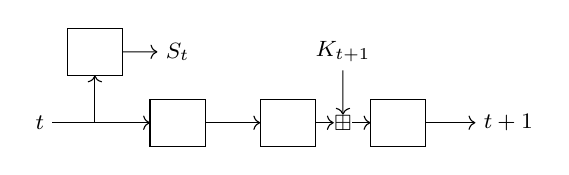
\begin{tikzpicture}[xscale=0.7,yscale=0.6]
      \footnotesize
      % variables
      \draw ( 2, 0) node(Xt){$\fsmState{t}$} ;
      \draw (10.5, 0) node(Xtplus){$\fsmState{t+1}$} ;
      \draw (7.5, 1.5) node(Kt){$K_{t+1}$} ;
      \draw (4.5, 1.5) node(St){$S_t$};
      % operations
      \draw (2.5, 1) rectangle (3.5, 2) node[pos=0.5]{$\filter$} ;
      \draw ( 4, -0.5) rectangle (5, 0.5) node[pos=0.5]{$\shiftR$} ;
      \draw ( 6, -0.5) rectangle (7, 0.5) node[pos=0.5]{$\mixC$} ;
      \draw ( 7.5, 0) node(add)[inner sep=0pt]{$\boxplus$} ;
      \draw (8, -0.5) rectangle (9, 0.5) node[pos=0.5]{$\subW$} ;
      % arrows
      \draw[->] (Xt) -- (4, 0) ;
      \draw[->] (3, 0) -- (3, 1) ;
      \draw[->] (3.5, 1.5) -- (St) ;
      \draw[->] (5, 0) -- (6, 0) ;
      \draw[->] (7, 0) -- (add) ;
      \draw[->] (Kt) -- (add) ;
      \draw[->] (add) -- (8, 0) ;
      \draw[->] (9, 0) -- (Xtplus) ;
    \end{tikzpicture}
    \caption{\label{fig:notations}Notation throughout clocks.}
  \end{subfigure}
  \hfill
  \begin{subfigure}[t]{0.34\textwidth}
    \centering
    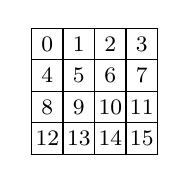
\begin{tikzpicture}[xscale=0.4,yscale=0.4]
      \footnotesize
      \foreach \i in {0,1,2,3}{
        \foreach \j in {0,1,2,3}{
          \draw (\i,\j) rectangle (\i+1,\j+1) ;
        }
      }
      \draw (.5,3.5) node {$0$};
      \draw (1.5,3.5) node {$1$};
      \draw (2.5,3.5) node {$2$};
      \draw (3.5,3.5) node {$3$};

      \draw (.5,2.5) node {$4$};
      \draw (1.5,2.5) node {$5$};
      \draw (2.5,2.5) node {$6$};
      \draw (3.5,2.5) node {$7$};

      \draw (.5,1.5) node {$8$};
      \draw (1.5,1.5) node {$9$};
      \draw (2.5,1.5) node {$10$};
      \draw (3.5,1.5) node {$11$};

      \draw (.5,.5) node {$12$};
      \draw (1.5,.5) node {$13$};
      \draw (2.5,.5) node {$14$};
      \draw (3.5,.5) node {$15$};
    \end{tikzpicture}
    \caption{\label{fig:numbering}Numbering in the FSM.}
  \end{subfigure}
  \hfill~
  
  \caption{\label{fig:notations-all}Our notations. Note that the numbering of the digits differs from the one traditionally used for the \gls{AES}.}
\end{figure}


% Leo: ce qui suit est pour qu'emacs compile bien l'article, pas touche !
%%% Local Variables:
%%% mode: latex
%%% ispell-local-dictionary: "english"
%%% TeX-master: "../main"
%%% End:







\paragraph{S-box Layer ($\subW$).}
We let $\thesbox$ be defined by its lookup table:
\begin{equation}
  \label{eq:thesbox}
  \thesbox = {\tt [1, 12, 6, 11, 14, 3, 15, 5, 10, 9, 13, 16, 7, 8, 0, 2, 4]}
\end{equation}
so that $\thesbox(0) = 1$, $\thesbox(1) = 12$, and so on. It has the following polynomial representation, and is thus of maximum degree: %\jb{il y a un $13x^{10}$  dans le polynome. C'est un $13x^{10}$ ?}\lp{oui}
\begin{equation*}
  \begin{split}
    \thesbox(x) ~=~& 1 + 4 x^{1} + 13 x^{2} + 7 x^{3} + 16 x^{4} + 15 x^{5} + 5 x^{7} + 5 x^{8} \\
    & + 11 x^{9} + 13 x^{10} + 12 x^{11} + 13 x^{12} + 15 x^{14} + x^{15}~.
  \end{split}
\end{equation*}
It was chosen by enumerating all APN permutations of $\mathbb{F}_{17}$, i.e., all permutations $A$ such that the equation $A(x+a)=A(x)+b$ has at most 2 solutions $x$ for all $a \neq 0$ and all $b$. Then, we selected $\thesbox$ among those that offer a good balance between minimizing the number of pairs $(a,b)$ for which the previous equation has exactly two solutions, and minimizing the maximum modulus of the Walsh spectrum (see Definition~\ref{def:fourier}).


\paragraph{Linear Layer ($\mixC$).} We opted for a $4 \times 4$ Maximum Distance Separable (MDS) matrix to ensure optimal diffusion. The matrix we chose is 
\begin{equation}
  \label{eq:mixmat}
  \mixmat = \left[ { \tiny
      \begin{array}{rrrr}
        2 & 1 & 1 & 1 \\
        1 & -1 &1 & -2 \\
        1 & 1 & -2 &-1 \\
        1 & -2 &-1 &1 \\
      \end{array}
    }\right]~.
   % \begin{array}{cccc}
    %  -1 & -1 & -1 & 2 \\
     % -1 & 1 & 2 & -1 \\
     % -1 & 2 & 1 & 1 \\
     % 2 & 1 & -1 & 1 \\
   % \end{array} \right]~.
\end{equation}
%We obtained it by performing an exhaustive search of all $4 \times 4$ matrices with coefficients in ${-2,-1,1,2}$ with at most one coefficient 2 or -2 in each row, and then picking one with the smallest $\ell_2$-norm for a matrix with coefficients in $\mathbb{F}_{17}$. The idea with our initial restrictions to ensure that the $\ell_2$ norm will be low as it depends on the absolute value of the coefficients.

We verified that there is no MDS matrix in  $\mathbb{F}_{17}$ with coefficients in $\{-1,1\}$ by exhaustively  testing all such matrices. As we were interested in MDS matrices with minimal $\ell_2$-norm and we were able to find during the initial experiments  matrices with a squared $\ell_2$-norm of 7, it was evident from the definition of the $\ell_2$-norm that matrices with minimal $\ell_2$-norm could not have coefficients $x$ with $|x| > 2$.  Thus, by testing all matrices with coefficients in $\{-2,-1,1,2\}$, we found a total of $30\>720$ MDS matrices with an $\ell_2$-norm of 7. We selected $\mixmat$ for its symmetries, particularly because it is its own transpose. % Among them, some matrices had a more structured form, as they could be written as 

% \begin{equation*}
%   \mixmat = \left[
%   \begin{array}{rr}
%     A & B  \\
%     B & -A 
%   \end{array} \right]~.
% \end{equation*}
% where both $A$ and $B$ are $2\times 2$ matrices. There were in total 256 matrices of this particular form and we chose $M$ randomly among them, taking into account also that $\mixmat = \mixmat^{T}$.
% (which means its linear behaviour is close to its differential behaviour). \leo{À vérifier}\ac{Cette phrase est bizarre : les branch nb et la distribution des poids sont les memes pour les deux codes si le code est MDS. Donc je ne vois pas ce que cela apporte qu'ils soient identiques.} \leo{ok, j'ai viré}


\paragraph{Filter.} The filter function $\filter$ maps $\mainField^{16}$ (i.e., the full FSM state) to a tuple $(a,b,c,d)$ in $\mainField^{4}$. As summarized in Figure~\ref{fig:filter}, we have that $a,b,c$ and $d$ correspond to the digits of the FSM state with indices 4, 6, 12, and 14 respectively (using the numbering from Figure~\ref{fig:numbering}).


\paragraph{LFSRs.} The whitening LFSR $\whitening$ and the key schedule LFSR $\pseudoKS$ are simply LFSRs over \(\F_p\) of maximum period, and have length 32 and 64 respectively. We obtain a
  maximum-period LFSR over $\mainField^w$ using the coefficients of a
  primitive polynomial as the taps.  More precisely, we used the {\tt SageMath}
  implementation of the finite field $\F_{p^w}$, which resulted in a pseudo-Conway polynomial. The output of the LFSR is taken from its last cell.

  More precisely, an LFSRs of length $\ell$ at time $t$ is a list of digits ${x^t_0, ..., x^t_{\ell-1}}$
  that is clocked as follows:
  \begin{enumerate}
  \item $x_0^{t+1} \gets - \sum_{i=0}^{\ell-1} x_i^t c_i$,
  \item $x_{i}^{t+1} \gets x_{i-1}^t$ for $0 < i < \ell$,
  \item the output is $x_{\ell-1}^t$,
  \end{enumerate}
  where $C=(c_i)_{0 \leq i < \ell}$ is the list of its taps, each being
  a digit of $\mathbb{F}_{17}$. We define $\clock{C}$ to be the function
  applying the operations above to a list ${x^t_0, ..., x^t_{\ell-1}}$
  to update it, and returning $x_{\ell-1}^t$.

  For the key schedule $\pseudoKS$, we use the following taps:
  \begin{equation*}
    \footnotesize
    \begin{split}
      C(\pseudoKS) ~=~& \{9, 4, 6, 4, 8, 6, 6, 16, 3,
                        9, 15, 12, 8, 12, 11, 4, 4, 8, 1,
                        8, 8, 9, 4, 6, 6, 7, 6, 3, \\
                      & 16, 14, 14, 6, 10, 15, 14, 13, 10, 1, 1,
                        10, 13, 11, 14, 10, 7, 4, 15, 8, 16,
                        3, 13, \\
                      & 14, 15, 16, 3, 16, 9, 3, 6,
                        12, 15, 9, 12, 3\}~,
    \end{split}
  \end{equation*}
  and for the whitening LFSR $\whitening$ we use
  \begin{equation*}
    \footnotesize
    \begin{split}
      C(\whitening) ~=~& \{8, 14, 14, 14, 1, 6, 12, 10, 14, 14,
                         14, 5, 2, 5, 6, 13, 6, 15, 14, 3, \\
                       & 13, 16, 1, 13, 9, 1, 7, 15, 13, 6,
                         14, 3\}~.
    \end{split}
  \end{equation*}


\paragraph{Master Key Processing.}
We generate the digits in $\pseudoKS$ first, and then those in $\whitening$. To generate them, we concatenate the 128-bit long master key with an IV and then a byte set to 1. The result is fed into \textsf{SHAKE128}, and the output byte stream of this primitive is used to generate digits of $\mathbb{F}_{17}$ using rejection sampling: if a byte $x$ is equal to 255, we discard it; otherwise, we generate the digit $\lfloor x / 15 \rfloor$. Since $15 \times 17 = 255$, this results in an unbiased transformation.


% Leo: ce qui suit est pour qu'emacs compile bien l'article, pas touche !
%%% Local Variables:
%%% mode: latex
%%% ispell-local-dictionary: "english"
%%% TeX-master: "main"
%%% End:





\subsection{Controlling the Noise Evolution}% in the Homomorphic Evaluation}
\label{sec:rationale-controllin-noise}

We first detail the implementation of each building block of the scheme using \gls{TFHE}, as this is essential to justify our design choices and to understand the evolution of the noise throughout the cipher. We then use this discussion to explain how the noise influences the overall security and efficiency of \coolName.

\paragraph{LFSR.} A naive approach for implementing an LFSR  homomorphically would be to maintain an encrypted state, and update it by computing a linear combination with the feedback coefficients. However, this method would cause the noise in the state to accumulate over time, necessitating periodic use of \gls{PBS} operations to refresh and control the noise growth. For this reason we introduce the principle of the \emph{silent LFSR}. Every output of an LFSR is a linear combination of the digits in its initial state. By computing on the fly the coefficients of these linear combinations in clear, we can evaluate the output of the LFSR at every clock cycle without updating an encrypted version of the internal state. This way, the noise variance in the output of the silent LFSR remains stable over time. This principle is comparable to the approach of {\tt FLIP}~\cite{EC:MJSC16} and follow-up works, whereby a key state is queried without being updated. 

To bound the noise variance in the output of the silent LFSR, we consider the worst-case scenario in which all the coefficients in the linear combinations are of maximal absolute value, i.e., $\frac{p-1}{2}$.\footnote{Constant coefficients of $\mainField$ are encoded as integers of the interval $[-\frac{p-1}{2}, \frac{p-1}{2}]$ to minimize their absolute value and hence their impact on the noise.} The resulting noise variance is thus equal to the original noise variance multiplied by the worst-case squared $\ell_2$-norm. Specifically, in the output of the key schedule LFSR $\pseudoKS$ and of the whitening LFSR $\whitening$, the noise variances $\sigma_\pseudoKS^2$ and $\sigma_\whitening^2$ satisfy
\begin{equation}
  \sigma_\pseudoKS^2 \leq | \pseudoKS | \cdot \left(\frac{p-1}2\right)^2 \cdot \sigma_{\text{fresh}}^2 ~~~\text{and}~~~ \sigma_\whitening^2 \leq | \whitening | \cdot \left(\frac{p-1}2\right)^2 \cdot \sigma_{\text{fresh}}^2,
\end{equation}
where $\sigma_{\text{fresh}}^2$ is the noise variance of the encrypted key material in the LFSRs.

\paragraph{SubDigits.} Each digit of the state of the FSM goes through a \gls{PBS} that evaluates the permutation $\thesbox$. All PBSs can be evaluated in parallel for higher speed. We denote by $\sigma_{\text{\gls{PBS}}}^2$ the noise variance at the output of $\subWords$ for encrypted digits.


\paragraph{ShiftRows.} Since each digit in the state is encrypted in a separate ciphertext digit, this step involves simply rearranging the ciphertext digits within the state. Consequently, it incurs no additional noise growth and no performance impact.

\paragraph{MixColumns.} This operation involves a straightforward linear combination of the digits of the state. The matrix $\mixmat$ has been specifically constructed to minimize the $\ell_2$-norm, considering coefficients in $\F_{17}$. %, while also ensuring optimal diffusion.
From the homomorphic perspective, this choice is crucial, as the variance of the noise increases proportionally with the square of this $\ell_2$-norm, that we denote $L_{\mixC}$. Namely, the noise variance $\sigma^2_\mixC$ after  $\mixColumns$ satisfies $\sigma^2_\mixC = L_{\mixC }^2 \cdot \sigma_{\text{\gls{PBS}}}^2.$


\paragraph{Sums.} The output of $\mixColumns$ is then added to the next output of the LFSR to be injected again into $\subWords$. The noise variance after the addition step corresponds to the sum of both noise variances. Similarly, the noise variance at the output of the scheme, referred to as $\sigma^2_{\text{out}}$, is equal to the sum $\sigma_\whitening^2 + \sigma_{\text{\gls{PBS}}}^2$.
%\medskip


%!TeX root = ../../../thesis.tex
\def\yPseudoKS{-3}

\begin{figure}[t!]
  \centering
    \footnotesize
    \begin{tikzpicture} [xscale=1,yscale=0.45]
      % LFSR interactions
      \draw (-1, \yPseudoKS) rectangle ++(3, 1) node[pos=0.5]{$\pseudoKS$ {\tiny \emph{(Key Schedule)}}} ;
      \draw (-1, 2.5) rectangle (2, 3.5) node[pos=0.5]{$\whitening$ {\tiny \emph{(whitening LFSR)}}} ;
      \draw (3.5, \yPseudoKS + 0.5) node[inner sep=0pt](addm){$\boxplus$} ;

      \node at (0.5, \yPseudoKS - 1) {$\sigma_{\text{fresh}}^{2}$};
      \node at (0.5, \yPseudoKS - 2.5) {\scalebox{0.5}{\verticalgauge{10}}};
      \node at (0.5, 2) {$\sigma_{\text{fresh}}^{2}$};
      \node at (0.5, 0.5) {\scalebox{0.5}{\verticalgauge{10}}};

      \draw (2.7, \yPseudoKS) node[inner sep=0pt](varKS){$\sigma_\pseudoKS^2$} ;
      \node at ($(varKS.south) + (0, -1)$) {\scalebox{0.5}{\verticalgauge{30}}};
      
      \draw (4.5, 3.5) node[inner sep=0pt](varW){$\sigma_\whitening^2$} ;
      \node at ($(varW.north) + (0, 1)$) {\scalebox{0.5}{\verticalgauge{30}}};
      \draw (7, \yPseudoKS) node[inner sep=0pt](varPBS){$\sigma_{\text{\gls{PBS}}}^2$} ;
       \node at ($(varPBS.south) + (0, -1)$) {\scalebox{0.5}{\verticalgauge{50}}};
      \draw (9.7,\yPseudoKS) node[inner sep=0pt](varSR){$\sigma_{\text{\gls{PBS}}}^2$} ;
      \node at ($(varSR.south) + (0, -1)$) {\scalebox{0.5}{\verticalgauge{50}}};
      \draw (8, 2 * \yPseudoKS - 1) node[inner sep=0pt](varMC){$\sigma^2_\mixC$} ;
      \node at ($(varMC.south) + (0, -1)$) {\scalebox{0.5}{\verticalgauge{70}}};
      \draw (4.35, \yPseudoKS + 1.5) node(sum) {$\sigma_\pseudoKS^2+\sigma^2_\mixC$};
      \node at ($(sum.south) + (0, 2)$) {\scalebox{0.5}{\verticalgauge{70}}};
      \draw (9, 3.5) node[inner sep=0pt](varout){$\sigma^2_{\text{out}}  = \sigma_\whitening^2 + \sigma_{\text{\gls{PBS}}}^2$} ;
      \node at ($(varout.north) + (0, 1)$) {\scalebox{0.5}{\verticalgauge{50}}};

      \draw[->] (2, \yPseudoKS + 0.5) -- (addm) ;
      \draw[->] (2.5, \yPseudoKS + 0.5) -- (2.5, \yPseudoKS + 1.5) -- (0.5, \yPseudoKS + 1.5) -- (0.5, \yPseudoKS + 1) ;
      \draw[->] (2.5, 3) -- (2.5, 4) -- (0.5, 4) -- (0.5, 3.5) ;
      % FSM
      \draw[color=blue,style=dashed] (5, \yPseudoKS) rectangle ++(1, 1) node[pos=0.5]{$\subW$} ;
      \draw (8, \yPseudoKS) rectangle ++(1, 1) node[pos=0.5]{$\shiftR$} ;
      \draw (10.3, \yPseudoKS) rectangle ++(1, 1) node[pos=0.5]{$\mixC$} ;
      \draw[->] (addm) -- (5, \yPseudoKS + 0.5) ;
      \draw[->] (6, \yPseudoKS + 0.5) -- (8, \yPseudoKS + 0.5) ;
      \draw[->] (9, \yPseudoKS + 0.5) -- (10.3, \yPseudoKS + 0.5) ;
      \draw[->] (11.3, \yPseudoKS + 0.5) -- (11.6, \yPseudoKS + 0.5) -- (11.6, 2 * \yPseudoKS - 0.5) --  (3.5, 2 * \yPseudoKS - 0.5) -- (addm) ;
      % extracting
      \draw (6.5, \yPseudoKS + 3) rectangle ++(1, 1) node[pos=0.5]{$\filter$} ;
      \draw (7, 3) node[inner sep=0pt](addr){$\boxplus$};
      \draw(11.3, 3) node(s){$Z_i$} ;
      \draw[->] (2, 3) -- (addr) ;
      \draw[->] (7, \yPseudoKS + 0.5) -- (7, \yPseudoKS + 3) ;
      \draw[->] (7, \yPseudoKS + 4) -- (addr) ;
      \draw[->] (addr) -- (s) ;
      % wire width
      % \draw (4.45, -0.2) -- (4.55, 0.2) ;
      % \draw (4.5, -0.5) node{$m$} ;
      % \draw[color=lightgray] (4.45, 2.8) -- (4.55, 3.2) ;
      % \draw[color=lightgray] (4.5, 3.5) node{$r$} ;
    \end{tikzpicture}
    \caption{Evolution of the noise variance in a homomorphic evaluation of \coolName. Operations involving PBSs are in blue and dashed. The gauges allow to visualize the evolution of the noise on a logarithmic scale).}
    \label{fig:noise}
\end{figure}







Figure~\ref{fig:noise} illustrates the evolution of the noise variance throughout the operations of \coolName.
Building on the previous equations, the main constraints influencing the design of \coolName are related to the noise variance at both the input of the \gls{PBS} and the output of the scheme. Specifically, the noise variance $\sigma_\pseudoKS^2+\sigma^2_\mixC$ at the input of the \gls{PBS} (i.e., at input of $\subWords$) must remain sufficiently low, otherwise it could lead to a high probability of \gls{PBS} failure. Additionally, the noise variance $\sigma^2_{\text{out}}  = \sigma_\whitening^2 + \sigma_{\text{\gls{PBS}}}^2$ at the output stream must remain low enough for subsequent applications, ideally as close as possible to the nominal noise variance at the \gls{PBS} output $\sigma_{\text{\gls{PBS}}}^2$. In practical settings, we have $\sigma_{\text{\gls{PBS}}}^2 \gg \sigma_{\text{fresh}}^2$, the noise variances from both LFSRs are negligible compared to $\sigma_{\text{\gls{PBS}}}^2$. For example in our implementation, the noise magnitude of $\sigma_{\text{fresh}}$ is around $2^{14}$, while the noise magnitude of $\sigma_{\text{\gls{PBS}}}$ is around $2^{52}$. Consequently, $\sigma^2_{\text{out}} \approx \sigma_{\text{\gls{PBS}}}^2$ which validates the second constraint. Similarly, the noise variance at the input of the \gls{PBS} is close to that at the output of $\mixColumns$. The latter additionally remains low due to the minimized $\ell_2$-norm of the coefficients of the MDS matrix $\mixmat$, thereby validating the first constraint.


To wrap up, the design of \coolName{} allows to control the evolution of the noise in the FSM while getting a very low number of \gls{PBS} per element. To complete our noise analysis, we need to set the parameters of the \gls{TFHE} scheme to ensure the correctness of the \gls{PBS}. Concretely, the noise \( \sigma_\pseudoKS^2 + \sigma^2_\mixC \) at the input of \( \subWords \) should be low enough to fail with a negligible probability. Of course, these parameters must ensure that the \gls{PBS} operates as fast as possible while maintaining the security of the scheme. In Section~\ref{sec:tfhe-parameters}, we detail our method for selecting the parameters.





% Leo: ce qui suit est pour qu'emacs compile bien l'article, pas touche !
%%% Local Variables:
%%% mode: latex
%%% ispell-local-dictionary: "english"
%%% TeX-master: "main"
%%% End:




% !TeX root = ../../thesis.tex

\section{A Brief Summary of the Security Analysis}
\label{sec:security}

\coolName's full paper provides an extensive analysis of the security of the cipher. Even if these considerations are far from the topic of this manuscript, we provide in this section a brief overview of this analysis. We refer to the full paper \cite{transistor} for the developments of the proofs.


\paragraph{Time-Memory-Data Trade-Offs}

To dimension the size of the LSFR, we computed a bound to ensure that exhaustive attacks are out of reach even when leveraging trade offs with pre-computation and storage. 

Using $\pseudoKS = 64$ and $\whitening = 32$, the length of the keystream generated from the same key is limited to $2^{31}$ digits. As a result, TMDTO attacks have a time complexity of $2^{296}$ in the single IV-setting, which drops to $2^{130}$ when keystreams generated from $2^{130}$ IVs are available to the attacker.

\paragraph{Guess and Determine}

In this kind of attacks, the attacker links the FSM state $\fsmState{t}$ to the filter output $S_t$ and try to guess the key schedule $K_t$.

Based on an analysis of the filtering procedure of \coolName, we showed that in total the attacker has to guess $\frac{12}{16}|\pseudoKS|$ digits, leading to a complexity \( p^{\frac{3}{4} | \pseudoKS |} \approx 2^{196}\) without taking into account the whitening LFSR. If we consider it, the attacker first has to
guess its content, leading to an attack with complexity
\( p^{\frac{3}{4} | \pseudoKS | + | \whitening |} \approx 2^{294}\).
%


\paragraph{Three consecutive outputs are statistically independent of the secret key}

The basic strategy in (fast) correlation attacks against stream ciphers consists in recovering some information about (a part of) the initial state of the cipher from the knowledge of the keystream. 
In this context, an important quantity is the smallest length of output sequence $(S_t)_{t\in \N}$ that can provide information on the sequence produced by the key-LFSR. In the paper we prove that this length is 4, that is to say 3 consecutive outputs are statistically independent of the secret key. This is a very good performance with respect to the state of the art: the only other cipher with this property is \texttt{Rocca} \cite[Section 4.5]{ToSC:SLNKI21}. However, in this case this property has been derived from an automatic search method, while the structure of \coolName enables us to derive this argument in a very simple way from the MDS property of~$\mixColumns$. 


\paragraph{(Fast) Correlation Attacks Using Biased Linear Relations}


Our paper also provides an estimation of the minimal data complexity required to recover the internal state of the key-register from the knowledge of the output sequence $(S_t)_{t\in \N}$, given that at least four consecutive outputs $(S_t, S_{t+1}, S_{t+2}, S_{t+3})$ need to be considered together. Applying the so-called Xiao-Massey lemma \cite{add:XiaMas88,add:Bry89}, it is possible to see that as soon as the key-LFSR and the considered segment of the output sequence are not statistically independent, there exists a biased linear relation between the digits of these two sequences.

In the paper, we exhibit an upper bound on the correlation of such linear relation. This bound depends on the minimal number of active S-boxes over $n$ rounds, as well as the modulus of the Fourier coefficients of \coolName's S-box. We show that the design of our S-box brings the correlation down to a value small enough so that the amount of keystream that the attacker has to observe exceed the limit of $2^{31}$ digits fixed by TMDTO trade-offs.


\paragraph{Linear Distinguishers}

Another type of attack studied in the paper is linear distinguishing attacks \cite{EC:MeiSta88,EC:CanTra00,FSE:CheJohSme00,C:TIMAZ18}. These attacks do not recover the initial state of the key-register, but the counterpart is that they can use together several keystream segments produced from multiple initial state. They consist in exhibiting a biased linear relation among the keystream digits. Such a relation is typically derived from a \textit{parity-check equation} for the key-LFSR, defined by the multiples of the LFSR feedback polynomial. 

In \coolName's design, this polynomial has been chosen so that it shows good properties regarding the utility of these parity-check equations. The conclusion of our analysis is that such an attack would be more expensive than an exhaustive search for the key .


\medskip

The full security analysis also takes into account algebraic attacks; such that Gröbner basis or the use of annihilators of the filtering function.



\section{Performances of Transciphering with \coolName}
\label{sec:bench}


This section focuses on the performances of transciphering with \coolName. We first address the wrapping of a (\coolName) symmetric key as a compact set of \gls{TFHE} ciphertexts for which we additionally introduce a trade-off between bandwidth and computation. Next, we explain how to manage different data representations to be able to fit with the input format of the server application. We then provide a detailed description of the homomorphic evaluation of \coolName. We finally give some implementation benchmarks and comparison to the state of the art.

\subsection{Key Wrapping and Bandwidth in \gls{TFHE} Transciphering} \label{sec:key_wrapping}

Assume one wants to generate a fresh \gls{TFHE} ciphertext vector $(c_1, \ldots, c_t)$ for a plaintext vector $(m_1, \ldots, m_t) \in \mathbb{Z}_p^t$, where $c_i = (a_{i,1}, \ldots, a_{i,n}, b_i)$, for every $i \in [1,t]$. Since the $a_{i,j}$'s are uniformly sampled at random over $\mathbb{Z}_q$, a folklore trick is to generate them pseudorandomly from a seed. We get the following compressed encryption procedure (where $\lambda$ denotes the security level in bits):
  
\begin{center}
\noindent\framebox{
\begin{minipage}{0.8\textwidth}
\underline{$\mathtt{CompressEncrypt}(s,m_1, \ldots, m_t)$}
	\vspace{-2mm}
	\begin{enumerate}
	\item Sample $\mathsf{seed} \gets \{0,1\}^\lambda$
	\smallskip
	\item Expand $((a_{i,j})_{1 \leq j \leq n})_{1 \leq i \leq t} \gets \mathsf{PRG}(\mathsf{seed})$
	\smallskip
	\item $\forall \:i \in [1,t]$: $b_i \gets \sum_{j=1}^n a_{i,j} \cdot s_j + \tilde{m}_i + e_i$ with $e_i \gets \chi_{\sigma}$
	\smallskip
	\item Return $(\mathsf{seed}, b_1, \ldots, b_t)$
\end{enumerate}
\end{minipage}}
\end{center}

\smallskip

Recovering standard \gls{TFHE} ciphertexts $c_1$, \ldots, $c_t$ from the compressed form $(\mathsf{seed}, b_1, \ldots, b_t)$ is simply done by expanding the $a_{i,j}$'s from $\mathsf{seed}$. The size of the obtained compressed ciphertext vector is $\lambda + t \cdot \log_2(q)$ against $t \cdot (n+1) \cdot \log_2(q)$ for a standard \gls{TFHE} encryption, meaning a compression by a factor about $(n+1)$. 

This compressed \gls{TFHE} encryption method can be applied directly to transmit homomorphically encrypted data from the user to the server. Alternatively, it can be combined with transciphering to encrypt a symmetric key. The resulting bandwidth requirements and the corresponding plaintext-to-ciphertext expansion factor are summarized in Table~\ref{tab:formulas_bandwidth}, where they are further compared with the naive (uncompressed) \gls{TFHE} encryption. In particular, for \coolName, a wrapped key is of size $\lambda + (|\mathcal K| + |\mathcal W|) \cdot \log_2(q)$, (which in our case gives 784 bytes) for a security of $\lambda = 128$ bits (target security of \coolName), the standard choice of $q= 2^{64}$ (which we use in our implementation) and $|\mathcal K| + |\mathcal W| = 96$ per the specification of \coolName (see Section~\ref{sec:description}). This fixed cost is hence very quickly amortized while the amount of data to encrypt grows.
Moreover, this approach can be applied to the server keys as well, which are actually encryptions of the secret key's bits. We took this optimization into account in our estimations of the server key sizes in Table \ref{tab:server_key_size}. 

\paragraph{Compressing further.}

We introduce hereafter a tweak to compress a \gls{TFHE} encryption further than the folklore compression. By definition of the \gls{TFHE} encryption process, the least significant bits of the body $b_i = \sum_{j=1}^n a_{i,j} \cdot s_j + \tilde{m}_i + e_i$ are randomized by the error $e_i$ and can hence be discarded without loss of information. We can thus tweak the above compressed encryption process by returning $(\mathsf{seed}, \mathrm{Tr}_\ell(b_1), \ldots, \mathrm{Tr}_\ell(b_t))$ where $\mathrm{Tr}_\ell(\cdot)$ denotes the truncation of the $\ell$ least significant bits. To decompress such ciphertexts, besides pseudorandomly generating the masks from the seed, one just needs to pad the truncated bodies with $\ell$ bits to $0$. By the randomness of the mask, the effect of this truncation plus $0$-padding is to add a uniform random error of $\ell$ bits to the body, namely an error of standard deviation: 
$$\sigma_0^2  = \frac{(2^\ell - 1)^2}{12} \approx \frac{2^{2\ell}}{12} \approx 0.08 \cdot 2^{2\ell} ~.$$

\noindent This optimization comes in two flavors:
\begin{enumerate}
	\item \emph{The ``free'' variant.} The number of truncated bits $\ell$ is selected to have a small impact on the noise distribution. For instance in \coolName, the noise of the fresh ciphertexts is summed with the noise coming from the FSM. Thus, we can compute $\ell$ to keep $\sigma^2_{\mathcal W} < \sigma^2_{\text{\gls{PBS}}}$. Our experiments shows $\sigma^2_{\text{\gls{PBS}}} = 2^{52}$, so running the numbers we find that we can truncate up to $\ell=19$ bits, allowing to reduce the volume of the \gls{TFHE} ciphertexts to send by a factor $1 - \frac{19}{64} \approx 0.7$.
	
	\smallskip
	
	\item \emph{The communication-computation trade-off.} In this variant, one selects a high value of $\ell$. The truncated body should at least contain $\log_2(p)$ bits to keep the plaintext information, plus a margin of a few bits in order to remain bootstrappable. Denoting this margin $\delta$, the truncated body should be of at least $\log_2(p) + \delta$ bits and $\ell$ can be up to $\log_2(q) - (\log_2(p)+\delta)$. Taking the maximum level of truncation, inducing the maximum level of bootstrappable noise, implies some adaptation of the underlying homomorphic computation. Specifically, it should start with applying a noise-reduction bootstrapping to the decompressed ciphertexts before performing the original evaluation. We hence obtain a trade-off with reduced bandwidth against additional bootstrappings.
\end{enumerate}

In the context of transciphering with \coolName, the trade-off provided by the second option gives rise to an initialization procedure which consists in decompressing and bootstrapping the wrapped key. 

This kind of compression has been more extensively studied in the concurrent work \cite{EPRINT:BCCS24}.

\begin{table}[t!]
	\centering
        \caption{Bandwidth of homomorphic ciphertexts (in bits).}
        % The total bandwidth is the fixed cost + $t$ times the cost per message to encrypt $(m_1, \ldots, m_t)\in \mathbb{Z}_p^t$.
	\label{tab:formulas_bandwidth}
        {
          \renewcommand{\arraystretch}{1.1}
          \footnotesize
          \scalebox{0.9}{
            \begin{tabular}{|l|*{3}{>{\centering\arraybackslash}p{3.5cm}|}}
              \hline
              \textbf{Approach used} & \textbf{Naive} & \textbf{Compressed} & \textbf{\coolName} \\
              \hline
              Fixed cost & 0 & $\lambda$ & $\lambda + (|\mathcal{K}|+|\mathcal{W}|) \cdot \log_2(q)$ \\
              \hline
              Per message in $\mathbb{Z}_p$ & $(n+1) \cdot \log_2(q)$ & $\log_2(q)$ & $\log_2(p)$ \\
              \hline
              Expansion factor~ & $(n+1) \cdot {\log_2(q)}/{\log_2(p)}$ & ${\log_2(q)}/{\log_2(p)}$ & 1 \\
              \hline
            \end{tabular}}
        }
	
\end{table}



\subsection{Transciphering vs. Data Representation}
\label{sec:data_representation}

Managing data representation is a common challenge when working with \gls{TFHE}. Since this scheme is only efficient at very low precision, an abstraction layer is required to construct practical data types (e.g., 8-, 32-, or 64-bit integers) from smaller encrypted chunks. Common constructions include radix-based decompositions and Chinese Remainder Theorem (CRT) representations, leading to different efficiency trade-offs. Carry propagation in radix-based representations is notoriously slow due to the large number of required bootstrappings, while CRT representations impose constraints on feasible operations. These constructions have been studied in~\cite{JC:BBBCLO23}. 

As a result, there is no universal representation that is optimal for all homomorphic operations. Thankfully, the representation of data in the transciphering algorithm can be chosen independently of that of the homomorphic application running on the server. If the representation in $\mathbb Z_p$ does not suit the application, the server can convert the ciphertexts to the desired representation before running the application. %Such a conversion can be either applied to the \gls{TFHE} ciphertexts obtained by the server after transciphering, or directly on the keystream (in this case, the symmetric ciphertexts are encoded directly in the desired representation, and the encryption/decryption operation is performed in the corresponding space). In both cases, it simply requires a bootstrapping for each element of $\mathbb Z_p$. 
We stress that this additional step of conversion would be necessary for any transciphering algorithm, as the data format desired in output of transciphering is completely application-dependent.

	
As a concrete example, assume that the data to be encrypted (i.e., the input to the homomorphic computation) consists of elements from $\mathbb{Z}_{16}$. The overall transciphering process unfolds as follows. On the client side, the plaintext is first embedded from $\mathbb{Z}_{16}$ into $\mathbb{Z}_{17}$ before being encrypted using \coolName. On the server side, the keystream is homomorphically generated and then used to homomorphically decrypt the ciphertext. This results in a \gls{TFHE} encryption of the original plaintext, now embedded in $\mathbb{Z}_{17}$, meaning that the plaintext space for the \gls{TFHE} encryption is $\mathbb{Z}_{17}$. A programmable bootstrapping (\gls{PBS}) operation is then applied to switch the plaintext space from $\mathbb{Z}_{17}$ back to $\mathbb{Z}_{16}$.

In terms of computation, this process adds one \gls{PBS} per $\mathbb{Z}_{16}$-element of the original plaintext, in addition to the four \gls{PBS} per element required for keystream generation with \coolName. Moreover, embedding $\mathbb{Z}_{16}$ into $\mathbb{Z}_{17}$ increases the size of the encrypted data by a factor of $1 + 1/16 = 1.0625$.

This approach can be generalized to address other plaintext representations. In particular, for larger chunks of bits, the bootstrapping operation would allow to merge several elements of $\mathbb{Z}_{16}$ (embedded into $\mathbb{Z}_{17}$) into one element of $\mathbb{Z}_{2^\ell}$ with $\ell > 4$. On the other hand, one may split an element of $\mathbb{Z}_{16}$ (or its $\mathbb{Z}_{17}$ embedding) into 4 elements of $\mathbb{Z}_{2}$ using a \gls{PBS} with multiple look-up tables (``PBSmanyLUT'') as proposed in~\cite{AC:CLOT21}.



	
\subsection{Detailed Homomorphic Implementations}
\label{sec:detailed_implementation}

In the following, we provide a more detailed way of how we implemented the homomorphic version of \coolName.

\paragraph{Homomorphic evaluation of LFSRs.}
The \coolName design involves two LFSRs operating on elements of $\F_{17}$. The standard way to implement an LFSR is to evaluate the linear feedback function on the state at each clock cycle, thus producing a new element that enters the state, while the state is shifted to output an element. 

We suggest the \emph{silent LFSR} approach for the homomorphic evaluation of LFSRs. In this approach, the encrypted LFSR state is immutable to avoid any noise growth in the underlying ciphertexts (hence keeping the LFSR ``silent''). We use the fact that every output element of the LFSR can be expressed as a linear combination of the initial state. So, at each clock cycle, we compute \emph{in the clear} the coefficients of this linear combination and homomorphically evaluate it on the immutable encrypted state. This process is depicted in Algorithm~\ref{alg:lsfr}.


\begin{algorithm}[t!]
    \caption{\texttt{LFSR.clock} - Produce a pseudo random element of the state. \label{alg:lsfr}}
    
    \KwIn{
        $\left\{
        \begin{aligned}
            &\ell: \text{ Size of the state of the LFSR.} \\
            &(u_1, \dots, u_\ell): \text{ Encrypted initial state of the LFSR.} \\
            &(\lambda_1^{(0)}, \dots, \lambda_\ell^{(0)}): \text{ Coefficients of retroaction in the definition of the LFSR.} \\
            &(\lambda_1^{(i)}, \dots, \lambda_\ell^{(i)}): \text{ Previous coefficients used in the linear combination.}
        \end{aligned}
        \right.$
    }

    \KwResult{
        $\left\{
        \begin{aligned}
            &o^{(i)}: \text{ Encryption of the $i$-th pseudorandom element of $\F_{17}$.} \\
            &(\lambda_1^{(i+1)}, \dots, \lambda_\ell^{(i+1)}): \text{ Updated coefficients of the linear combination.}
        \end{aligned}
        \right.$
    }

    % Add vertical space and horizontal line
    \vspace{0.5em} % adjust the space as needed
    \hrule
    \vspace{0.5em} % adjust the space as needed

    $o^{(i)} \gets 0$

    \Comment{Evaluation of the linear combination}
    \For{$k \in \{1, \dots, \ell\}$}{
        $o^{(i)} \gets \texttt{SumTFHE}(o^{(i)}, \texttt{ClearMultTFHE}(u_k, \lambda_k^{(i)}))$
    }
    \Comment{Update of the next coefficients}
    \For{$k \in \{2, \dots, \ell\}$}{
        $\lambda_k^{(i+1)} \gets \lambda_{k-1}^{(i)} + \lambda_\ell^{(i)} \cdot \lambda_k^{(0)}$
    }
    $\lambda_1^{(i+1)} \gets \lambda_\ell^{(i)} \cdot \lambda_1^{(0)}$
    
    \Return{$o^{(i)}$}
    
\end{algorithm}




\paragraph{Homomorphic evaluation of} \coolName. The complete homomorphic evaluation of a round of on clock cycle of \coolName is depicted in Algorithm~\ref{alg:transistor}, using $\pseudoKS.\texttt{clock}$ and $\whitening.\texttt{clock}$ as subroutines (i.e., Algorithm~\ref{alg:lsfr} evaluated on the key schedule and whitening LFSRs). The most computation intensive part of the algorithm is by far the evaluation of the \gls{PBS} in $\subWords$ which can be fully parallelized to reduce the latency.


 \begin{algorithm}[t!]
    \caption{\texttt{Transistor.clock} - Produce $r$ encypted elements of the key stream}
    \label{alg:transistor}
    
 
    \KwIn{
        $\left\{
        \begin{aligned}
        	&\mathcal K: \text{the LFSR used for the pseudo-keyschedule and its state (cf Algorithm \ref{alg:lsfr}).}\\
            &\mathcal W: \text{the LFSR used for the whitening.}\\	
            &X = \left ( \begin{array}{ccc}
            x_{1,1} & \dots & x_{1,\sqrt{m}}\\
            \dots & \dots & \dots\\
            x_{\sqrt{m},1} & \dots & x_{\sqrt{m},\sqrt{m}}\\
            \end{array} \right ): \text{ Encrypted state of the FSM} \\
        \end{aligned}
        \right.$
    }

    \KwResult{
        $\left\{
        \begin{aligned}
            &Y = (y_1, \dots, y_r): \text{ Encryption of $r$ elements of the  key stream } \\
        \end{aligned}
        \right.$
    }

    % Add vertical space and horizontal line
    \vspace{0.5em} % adjust the space as needed
    \hrule
    \vspace{0.5em} % adjust the space as needed

    \Comment{Compute the pseudo-key schedule and adds it to the FSM}
    \For{$i \in [1, \sqrt m]$}{
        \For{$j \in [1, \sqrt m]$}{
            $k_{i,j} \gets \pseudoKS.\texttt{clock}()$\\
            $x_{i,j} \gets \texttt{SumTFHE}(x_{ij}, k_{i,j})$\\
        }
    }
    \Comment{Compute $\subWords$ with a layer of PBS}
    \For{$i \in [1, \sqrt m]$}{
        \For{$j \in [1, \sqrt m]$}{        
            $x_{i,j} \gets \texttt{PBS\_TFHE}(x_{i,j}, S)$\\
        }
    }
    \Comment{Extract the output bits and whiten them}
    $(y_1, \dots, y_r) \gets \phi(X)$\\
    \For{$i \in [1, r]$}{
        $w_i \gets \whitening.\texttt{clock}()$\\
        $y_i \gets \texttt{SumTFHE}(y_i, w_i)$\\
    }
    \Comment{Compute $\shiftRows$, (same as in clear)}
    $X \gets \shiftR(X)$

    \Comment{Compute MixColumns}
    \For{$i \in [1, \sqrt m]$}{
        \For{$j \in [1, \sqrt m]$}{
            $z_{i, j} \gets 0$\\
            \For{$k \in [1, \sqrt m]$}{
                $z_{i, j} \gets \texttt{SumTFHE}(z_{i, j}, \texttt{ClearMultTFHE}(x_{k, j}, MC_{i, k}))$\\
            }
        }
    }

    \Return{$Y$}

\end{algorithm}






\subsection{\gls{TFHE} Parameters} 
\label{sec:tfhe-parameters}


We discuss hereafter the selection of the different \gls{TFHE} parameters involved in the homomorphic implementation of \coolName. An extensive presentation of the \gls{TFHE} parameters and their role within the scheme can be found in Section \ref{sec:about_problem}.

Figure \ref{fig:structure_fhe} shows the ciphertext format at the different steps of the homomorphic evaluation of \coolName. It shows that the manipulated ciphertexts can be of three different types: LWE ciphertexts of dimension $n_{\text{short}}$, LWE ciphertexts of dimension $n_{\text{long}}$, or GLWE ciphertexts of dimension $k$ and polynomial degree $N$.
	

\begin{figure}[t!]
  \centering
    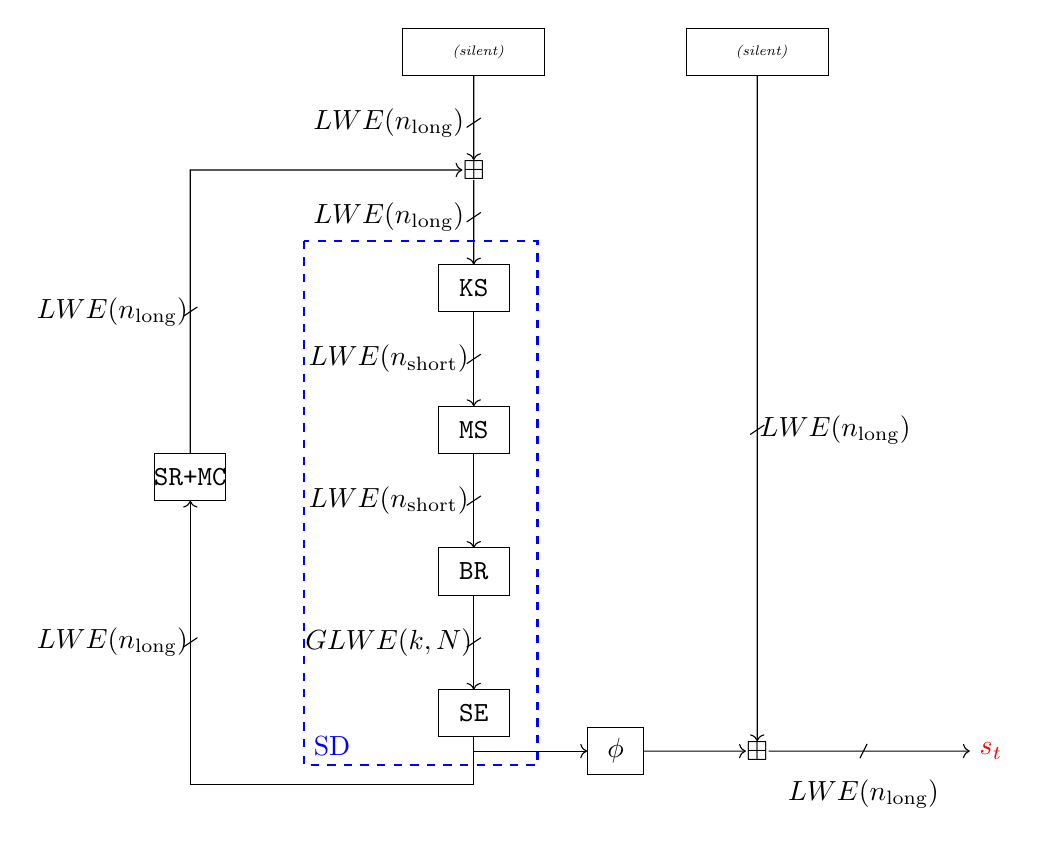
\begin{tikzpicture}[xscale=0.9,yscale=0.6]
 
    %LSFRs
    \draw[] (0, 0) rectangle (2, 1) node[pos=0.5]{$\pseudoKS$ {\tiny \emph{(silent)}}} ;
    \draw[] (4, 0) rectangle (6, 1) node[pos=0.5]{$\whitening$ {\tiny \emph{(silent)}}} ;
    \draw (1, -2) node[inner sep=0pt](addm){$\boxplus$} ;
    \draw[->] (1, 0) -- (addm);

    % FSM
    \draw[] (0.5, -4) rectangle (1.5, -5) node[pos=0.5,color=black](ks){$\texttt{KS}$} ;
    \draw[] (0.5, -7) rectangle (1.5, -8) node[pos=0.5,color=black](ms){$\texttt{MS}$} ;
    \draw[] (0.5, -10) rectangle (1.5, -11) node[pos=0.5,color=black](br){$\texttt{BR}$} ;
    \draw[] (0.5, -13) rectangle (1.5, -14) node[pos=0.5,color=black](se){$\texttt{SE}$} ;
    \draw[] (-3.5, -8) rectangle (-2.5, -9) node[pos=0.5,color=black](srmc){$\texttt{SR+MC}$} ;

    % Draw dashed blue box for SB
    \draw[dashed, blue, thick] (-1.4, -3.5) rectangle (1.9, -14.6);
    \node[blue] at (-1, -14.2) {SD}; % Label for the box

    % FSM connections
    \draw[->] (addm) -- (1, -4);
    \draw[->] (1, -5) -- (1, -7);
    \draw[->] (1, -8) -- (1, -10);
    \draw[->] (1, -11) -- (1, -13);
    \draw[->] (1,-14) -- (1, -15) -- (-3, -15) -- (-3, -9);
    \draw[->] (-3, -8) -- (-3, -2) -- (addm);

    % Extraction
    \draw (5, -14.3) node[inner sep=0pt](addr){$\boxplus$} ;
    \draw[] (2.6, -13.8) rectangle (3.4, -14.8) node[pos=0.5,color=black]{$\phi$} ;

    \draw[->] (1, -14.3) -- (2.6, -14.3);
    \draw[->] (3.4, -14.3) -- (addr);
    \draw[->] (5, 0) -- (addr);
    \draw[->] (addr) -- (8, -14.3);
    \draw[color=red] (8.3, -14.3) node(s){$s_t$} ;



    % Wire type
    \draw (0.9, -1.1) -- (1.1, -0.9) ;
    \draw (-0.2, -1) node{$LWE(n_{\text{long}})$} ;
    \draw (0.9, -3.1) -- (1.1, -2.9) ;
    \draw (-0.2, -3) node{$LWE(n_{\text{long}})$} ;
    \draw (0.9, -6.1) -- (1.1, -5.9) ;
    \draw (-0.2, -6) node{$LWE(n_{\text{short}})$} ;
    \draw (0.9, -9.1) -- (1.1, -8.9) ;
    \draw (-0.2, -9) node{$LWE(n_{\text{short}})$} ;
    \draw (0.9, -12.1) -- (1.1, -11.9) ;
    \draw (-0.2, -12) node{$GLWE(k, N)$} ;
    \draw (-3.1, -12.1) -- (-2.9, -11.9) ;
    \draw (-4.1, -12) node{$LWE(n_{\text{long}})$} ;
    \draw (-3.1, -5.1) -- (-2.9, -4.9) ;
    \draw (-4.1, -5) node{$LWE(n_{\text{long}})$} ;
    \draw (4.9, -7.6) -- (5.1, -7.4) ;
    \draw (6.1, -7.5) node{$LWE(n_{\text{long}})$} ;
    \draw (6.45, -14.45) -- (6.55, -14.15) ;
    \draw (6.5, -15.2) node{$LWE(n_{\text{long}})$} ;

    \end{tikzpicture}
  \vspace{1em}
  \hfill~
  \caption{\label{fig:structure_fhe} Types and shapes of ciphertexts in homomorphic \coolName. The $\subWords$ is broken down into its elementary components}
\end{figure}


% Leo: ce qui suit est pour qu'emacs compile bien l'article, pas touche !
%%% Local Variables:
%%% mode: latex
%%% ispell-local-dictionary: "english"
%%% TeX-master: "../main"
%%% End:






\paragraph{Optimization of the \gls{TFHE} parameters.}
To generate a set of parameters, we use the method developed in~\cite{JC:BBBCLO23}. Given the negligible noise contribution from the LFSRs, the FSM can be modeled using the \emph{atomic pattern} introduced in~\cite{JC:BBBCLO23} (specifically the instance referred to as $\mathcal{A}^{(\text{CJP21})}$), which is a pattern of homomorphic operators taking a set of ciphertexts in input, computing linear combinations of those ciphertexts and applying a programmable bootstrapping to each of them. The FSM round in \coolName which composes a multiplication by a constant matrix ($\mixColumns$), followed by a bootstrapping step ($\subWords$) is precisely an instance of such an atomic pattern. The framework proposed in~\cite{JC:BBBCLO23} generates parameters that guarantee a specified security level $\lambda$ for the LWE encryption and target error probability $p_{\text{err}}$, while optimizing the \gls{PBS} to be as fast as possible. 

Table \ref{tab:transistor_parameters} shows the parameters used for our experiments, all ensuring 128 bits of security. The obtained security levels $\lambda_{\text{short}}$ et $\lambda_{\text{long}}$ have been estimated using the \texttt{lattice estimator}~\cite{lattice-estimator}.

\begin{table}[t!]
\centering
\caption{\gls{TFHE} Parameters used in our experiments}.
\label{tab:transistor_parameters}
\renewcommand{\arraystretch}{1.3}  % Adjust row spacing
\scalebox{1}{
	\begin{tabular}{|c||*{12}{>{\centering\arraybackslash}p{0.8cm}|}}
		\hline
		$p_{\text{err}}$ & $q$ & $n_{\text{short}}$ & $k$ & $N$ & $\sigma_{\text{short}}$ & $\sigma_{\text{long}}$ & $\baseDecompPBS$ & $\levelDecompPBS$ & $\baseDecompKS$ & $\levelDecompKS$ & $\lambda_{\text{short}}$ & $\lambda_{\text{long}}$\\
		\hline
		$2^{-40}$ & $2^{64}$ & 788 & 2 & 1024 & $2^{47}$ & $2^{14}$ & $2^{23}$ & 1 & $2^4$ & 3 & 131.8 & 128.9\\
		\hline
		$2^{-128}$ & $2^{64}$ & 774 & 1 & 2048 & $2^{47}$ & $2^{14}$ & $2^{23}$ & 1 & $2^3$ & 5 & 131.8 & 128.9\\
		\hline
\end{tabular}
}
	\end{table}



\paragraph{Encryption security.} 
The security level (in bits) of the LWE ciphertexts is a function of the modulus $q$, the dimension $n$ and the noise standard deviation $\sigma$. While no explicit formula exists for this function, the \emph{lattice estimator} tool allows to produce an estimation of this function by simulating the main attacks of the literature~\cite{lattice-estimator}, which we denote $\mathcal{O}$ (for \emph{security oracle}). The selected \gls{TFHE} parameters are constrained to satisfy $\mathcal{O}(q,n,\sigma) \geq \lambda$ for both $(q,n,\sigma) = (q,n_{\text{short}},\sigma_{\text{short}})$ and $(q,n,\sigma) = (q,n_{\text{long}},\sigma_{\text{long}})$.



\paragraph{Correctness of the \gls{PBS}.} To compute the error probability $p_{\text{err}}$, we have to evaluate the variances occurring inside the programmable bootstrapping of the $\subWords$ layer. This reasoning will be more detailed in Chapter \ref{chap:parameters} (with additional bits in Appendix \ref{sec:cjp_details}). Here, we provide a short reasoning sufficient for our purpose.


In the following, we denote the maximum error probability of the bootstrapping by $p_{\text{err}} := 2^{-\kappa}$. We aim to choose parameters such that the \gls{PBS} outputs a correct ciphertext with probability at least $1-p_{\text{err}}$. This translates to the following constraint:
$$\sigma^2_{\text{in-}\textsf{BR}} \leq  C(\kappa) \cdot \left(\frac1{4p}\right)^2 ~~~\text{with}~~~C(\kappa) := \left(\frac{1}{\sqrt{2} \cdot \mathsf{erfc}^{-1}(2^{-\kappa})}\right)^2 ~.$$
Under the Gaussian assumption, the noise in input of the \textsf{BlindRotate} is lower than $\mathsf{erfc}^{-1}(2^{-\kappa}) \cdot \sqrt{\sigma^2_{\text{in-}\textsf{BR}}}$ with probability $1-2^{-\kappa}$. The above constraint thus implies that, with probability $1-2^{-\kappa}$, the noise is lower than $1/{4p}$ which ensures the correctness of the \gls{PBS}. 

As $|\mathcal W| \leq |\mathcal K|$, we can check that we always have $\sigma^2_{\text{out}} \leq \sigma^2_{\text{in-}\textsf{\gls{PBS}}}$ which implies that the output is always bootstrappable with correctness probability at least $1-p_{\text{err}}$ in the subsequent bootstrapping.


\subsection{Performances} \label{sec:performances}

We provide hereafter some benchmarks of our implementation of \coolName for two sets of parameters tailored for two different error probabilities. We first consider $\perr = 2^{-40}$, which is a common choice in the literature to benchmark homomorphic implementations. Our results for this error probability allow a fair comparison with the state of the art. While such an error probability theoretically allows transciphering to be error-free with a large amount of data with good probability, some recent works have shown that non-negligible error probabilities could be exploited by an adversary in some contexts~\cite{C:CSBB24,CCS:CCPSS24}. Thus, we also provide another set of parameters and associated benchmark for $\perr =  2^{-128}$.

Our implementation relies on our customized version of \texttt{tfhe-rs}~\cite{tfhe-rs} which has been adapted to support odd $p$ (size of the plaintext space), that we described in Section \ref{sec:library}. The experiments were carried on a processor 12th Gen Intel(R) Core(TM) i5-1245U with 4.4 GHz. Table \ref{tab:perfs} summarizes the obtained timings for the two sets of parameters. The throughput is computed assuming that $\log_2(17)$ bits are encoded on one element of $\F_{17}$. Encoding 4 bits on each element would scale the throughput by a factor $4/\log_2(17) \approx 0.98$.

\begin{table}[t!]
	\centering
		\caption{Performances of our two instances of \coolName.}
	\label{tab:perfs}
	\renewcommand{\arraystretch}{1.2}  % Adjust row spacing
	\begin{tabular}{|c||*{3}{>{\centering\arraybackslash}p{3cm}|}}
		\hline
		~~$p_{\text{err}}$~~ & Time for one \gls{PBS} & Latency (one round) & Throughput\\
		\hline
		$2^{-40}$ & 11.9 ms & 195 ms & 83.84 bits/s\\
		\hline
		$2^{-128}$ & 15.28 ms & 251 ms & 65.10 bits/s\\
		\hline
	\end{tabular}
\end{table}



Although our current implementation does not leverage the inherent parallelism of \coolName, it is important to note that it can be easily parallelized across 16 threads. Specifically, during the $\subWords$ steps, which dominate the overall runtime, the 16 \gls{PBS} operations can be executed concurrently. This parallelization would result in nearly a 16-fold reduction in total execution time.

Without taking into account the server key\ifeprint(whose sizes are shown in Table \ref{tab:server_key_size})\fi, and using compressed encryption (Section \ref{sec:key_wrapping}),  transciphering 1 KB of plain data requires 1.78 KB of data to be sent, instead of 64 KB. For larger amounts of message, the volume of the encrypted symmetric key becomes negligible with respect to the message: for 1 MB of plain data, we use 1.0008 MB, and for 1 GB, this goes down to 1.000001 GB. The two sets of parameters yield the same bandwidth consumption, but not the same running time as shown in Table \ref{tab:perfs}.



By applying the ``free truncation optimization" introduced in Section \ref{sec:key_wrapping}, we can reduce the volume of the encrypted symmetric key by a factor~0.7. This is particularly useful when transciphering a small volume of data (the volume of the encrypted key being preponderant). For example, to transcipher 1 KB of data, using this technique decreases the volume from 1.78~KB to 1.54~KB. 

In Table \ref{tab:server_key_size} we provide the sizes for the server keys, namely the \emph{key-switching key} ($\KSK$) and the \emph{bootstrapping key} ($\BSK$) while using the ciphertext compression technique described in Section~\ref{sec:key_wrapping}. Those keys are only generated and communicated to the server once (during some user enrollment step).

\begin{table}[t!]
  \centering
  \caption{Size of the server keys for the two considered sets of parameters. 
    % This is agnostic to the volume of message sent. 
    \label{tab:server_key_size}}
  
  \renewcommand{\arraystretch}{1.2}  % Adjust row spacing
  \scalebox{0.9}{
    \begin{tabular}{|c||*{3}{>{\centering\arraybackslash}p{4cm}|}}
      \hline
      & Theoretical sizes & Sizes for $p_{\text{err}} = 2^{-40}$ & Sizes for $p_{\text{err}} = 2^{-128}$ \\
      \hline
      ~KSK~ &  $n_{\text{long}}\cdot l_{\text{KS}} \cdot \log_2 q $ & 49 KB & 82 KB  \\
      \hline
      ~BSK~ &  $n_{\text{short}} \cdot l_{\text{BS}} \cdot \log_2 q \cdot N \cdot (k+1)$ & 6.5 MB & 12.7 MB  \\
      \hline
    \end{tabular}
}
\end{table}




\subsection{Comparisons to the State of the Art}
\label{sec:perfs_soa}	

\subsubsection{Comparisons with other \gls{TFHE}-friendly ciphers.} 
%In Section \ref{sec:soa}, we provided an overview of the recent landscape of \gls{TFHE}-friendly symmetric ciphers.
In what follows, we compare \coolName with several of the most competitive state-of-the-art schemes. Our results are summarized in Table~\ref{tab:comparisons_soa}.
Although such comparisons must be interpreted with care — due to differences in libraries, hardware platforms, and bootstrapping error probabilities — they still offer valuable insights into the relative efficiency and trade-offs of these approaches.


In~\cite{DBLP:conf/wahc/BalenboisOS23}, \texttt{Trivium} and \texttt{Kreyvium} were evaluated on a powerful AWS instance, which makes direct comparison with our local experiments impractical. However, an important distinction is that \coolName requires no setup phase, unlike these ciphers. Also, the implementation optimizes the running time by switching between two sets of parameters, doubling the size of the evaluation keys.

\texttt{Margrethe}~\cite{EPRINT:AGHM24} has low noise ratios ($2^{-15.3}$ or $2^{-21.9}$), compared to around $2^{-12}$ for \texttt{Transistor}. Its authors also report low latencies of 27 or 54 ms, and high throughputs of 147 or 73 bits/s (depending on the configuration). However, these come at the cost of much larger sizes for the encryptions of the symmetric key. Indeed, the use of Vertical Packing mandates that symmetric keys be encrypted under $\GGSW$ form, resulting in hundreds of megabytes. Although an alternative (lifting from LWE to GGSW using circuit bootstrapping) could reduce the transmission size, it would significantly degrade performance. 

Similarly, Deo et al. proposed~\cite{EPRINT:DJLCB24} a pseudorandom function whose security relies on the hardness of the LWR problem~\cite{EC:BanPeiRos12}. It enables a stream cipher–like transciphering scheme, where each pseudorandom element in $\mathbb{Z}_p$ (with $p=2^5$) is produced using a single bootstrapping. Their implementation reaches up to 881 bits/s on their hardware, surpassing \texttt{Transistor} in throughput. However, as with \texttt{Margrethe}, this efficiency comes at the cost of a significant increase in key size: their PRF requires 500 to 1000 elements encrypted in GGSW form, which is much larger than the 96 elements in LWE form for \coolName.


The authors of \texttt{FRAST}~\cite{ToSC:CCHLOS24} implemented it with \texttt{tfhe-rs}, like \coolName. It targets 128-bit security with an error probability of $2^{-80}$. On the same platform, our instance of \coolName (with a tighter error bound of $2^{-128}$) achieves three times higher throughput, significantly lower latency, and does not require any setup phase—unlike \texttt{FRAST}, which involves a 25-second setup. In addition, \texttt{FRAST} requires substantially larger evaluation key material, due to its use of multiple derivatives of the \gls{PBS} algorithm. Finally, no information is provided regarding the output noise level of the scheme.



\begin{table}[t!]
	\centering
	\caption{Performance of state-of-the-art \gls{TFHE}-friendly ciphers (single-threaded when applicable). Communication cost accounts for both the encrypted symmetric key and the evaluation keys. \label{tab:comparisons_soa}}
	\resizebox{\textwidth}{!}{
	\renewcommand{\arraystretch}{1.3}  % Adjust row spacing
    \begin{tabular}{|c|c|c|c|c|c|}
		\hline
		Cipher & Setup & Latency & Throughput & Communication Cost\textsuperscript{a}  & $p_{\text{err}}$\\
		\hline
		\texttt{Trivium}~\cite{DBLP:conf/wahc/BalenboisOS23} (128 thr.) & 2259 ms & 121 ms & 529 bits/s & 640 B + 35.6 MB $\textsuperscript\dag$ & $2^{-40}$\\
		\hline
		\texttt{Kreyvium}~\cite{DBLP:conf/wahc/BalenboisOS23} (128 thr.) & 2883 ms & 150 ms & 427 bits/s & 1024 B + 35.6 MB $\textsuperscript\dag$ & $2^{-40}$\\
		\hline		
		\multirow{2}{*}{\texttt{Margrethe}~\cite{EPRINT:AGHM24}} & No & 27.2 ms & 147.06 bits/s & 64 MB \textsuperscript{*} & $<2^{-1000}$\\
		& No & 54.2 ms & 73.8 bits/s & 128 MB \textsuperscript{*} & $<2^{-1000}$\\
		\hline
		PRF-based construction~\cite{EPRINT:DJLCB24} & No &  5.675 ms & 881 bits/s & 32.8 MB = 8.9 MB + 23.9 MB & $2^{-64}$\\
		\hline
		\texttt{FRAST}~\cite{ToSC:CCHLOS24}  & 25 s (8 thr.) & 6.2 s & 20.66 bits/s & 34.05 MB = 148 KB + 33.91 MB & $2^{-80}$\\
		\hline
		~~\coolName~~  & No & 251 ms & 65.10 bits/s & 13.54 MB = 780 B + 12.78 MB & ~~$2^{-128}$~~\\
		\hline
	\end{tabular}
	}
	\begin{minipage}{\linewidth}
		\footnotesize\textsuperscript{*} In \texttt{Margrethe}, no keyswitching nor bootstrapping keys are required.\\
		\label{fn:margrethe_keysize}
		\footnotesize\textsuperscript{\dag} Values recomputed from the data of the papers. For consistency's sake, we applied the compression of ciphertexts of Section \ref{sec:key_wrapping} to estimate the communication cost.
		\label{fn:comm-cost}
	\end{minipage}
\end{table}


\subsubsection{Comparisons with other homomorphic schemes.} 
\gls{TFHE} yields very different trade-offs between the various performance metrics (latency, throughput, bandwith consumption, ...), compared to other \gls{FHE} schemes. In scenarios where throughput is a priority, \gls{TFHE}—and by extension, \texttt{Transistor}—is generally not the most suitable choice. However, \gls{TFHE} shines in use cases that require low-latency homomorphic computations and efficient evaluation of look-up tables (LUTs), thanks to its native support for fast programmable bootstrapping.
In the following, we provide a brief survey of some transciphering approaches built upon alternative homomorphic encryption schemes.

For CKKS-based transciphering, we look at the \gls{AES} evaluation using the so-called \texttt{XBOOT} optimization proposed in~\cite{EPRINT:NHYCKH25}. While the reported amortized throughput significantly outperforms that of \coolName, it comes at the cost of a much higher latency—153s and 236s using 64 threads, compared to 251ms for \coolName running on a single thread. We observe similar results for  BGV-based transciphering. In this case we instead consider the optimized evaluation of \texttt{RASTA}~\cite{C:DEGLLL18} presented in~\cite{EPRINT:NHYCKH25}. Using the same \texttt{XBOOT} optimization as the CKKS variant, it also yields high latencies: 303s, again with 64-thread parallelism. 


Lastly, \texttt{FINAL}~\cite{AC:BIPPS22} is another, more recent homomorphic encryption scheme based on NTRU. Its bootstrapping is approximately 30\% faster than \gls{TFHE}’s, but it is not programmable, and therefore does not support \gls{LUT} evaluation. The works~\cite{CiC:MeaParPer24,CCS:CDPP22} implement the stream cipher \texttt{Filip} using \texttt{FINAL}, relying on the Improved Filter Permutator paradigm, without LUTs' evaluation. The competitive performances of these implementations (resp. 159 bits/s and 381 bits/s) comes with a trade-off in key size: encrypting the symmetric key requires resp. 215 MB and 200 MB, versus 4.8 MB for \coolName~(uncompressed). This is mainly due to the size of the key register in \texttt{Filip} ($2^{14}$ bits), while \coolName~only requires the upload of 96 elements in~$\mathbb{Z}_{17}$ (around 400 bits).



\section{Conclusion}
\label{sec:conclusion}


\coolName{} is a new stream cipher design tailored to \gls{TFHE}
transciphering, that significantly outperforms the state-of-the-art of
\gls{TFHE}-friendly stream ciphers.  After analyzing the constraints of the
\gls{TFHE} setting in the context of a symmetric cipher, we designed
\coolName{} by combining an LFSR-based key schedule, an LFSR-based
whitening, and a non-linear FSM with an \gls{AES}-like structure.  We report
implementation results of \coolName{} using state-of-the-art \gls{TFHE}, using
a trick to implement \emph{silent} LFSRs.  This general structure can be
easily adapted to other contexts, and we believe it will find
applications beyond \gls{TFHE}.


One of the constraint of this design was that the cipher should work in a small plaintext space. This was because the bottleneck in terms of running time was the evaluation of the \gls{S-box}. But what if we could extend the capabilities of \gls{TFHE} and evaluates larger \gls{S-box}es, like in more conventional designs ?

This is the point of the next chapter, where we propose a construction to accelerate the evaluation of larger \gls{LUT}.




%\appendix
%\section{Full Specification of \coolName{}}
\label{app:spec}

%\newcommand\clock[1]{\mathsf{clock}_{#1}}

A reference implementation in {\tt Sage} is available online at
\begin{quote}
  \url{https://github.com/CryptoExperts/Transistor/}
\end{quote}


\subsection{LFSRs}
\label{app:spec-lfsrs}

An LFSRs of length $\ell$ at time $t$ is a list of digits ${x^t_0, ..., x^t_{\ell-1}}$
that is clocked as follows:
\begin{enumerate}
\item $x_0^{t+1} \gets - \sum_{i=0}^{\ell-1} x_i^t c_i$,
\item $x_{i}^{t+1} \gets x_{i-1}^t$ for $0 < i < \ell$,
\item the output is $x_{\ell-1}^t$,
\end{enumerate}
where $C=(c_i)_{0 \leq i < \ell}$ is the list of its taps, each being
a digit of $\mathbb{F}_{17}$. We define $\clock{C}$ to be the function
applying the operations above to a list ${x^t_0, ..., x^t_{\ell-1}}$
to update it, and returning $x_{\ell-1}^t$.

For the key schedule $\pseudoKS$, we use the following taps:
\begin{equation*}
  \footnotesize
  \begin{split}
    C(\pseudoKS) ~=~& \{9, 4, 6, 4, 8, 6, 6, 16, 3,
                      9, 15, 12, 8, 12, 11, 4, 4, 8, 1,
                      8, 8, 9, 4, 6, 6, 7, 6, 3, \\
                    & 16, 14, 14, 6, 10, 15, 14, 13, 10, 1, 1,
                      10, 13, 11, 14, 10, 7, 4, 15, 8, 16,
                      3, 13, \\
                    & 14, 15, 16, 3, 16, 9, 3, 6,
                      12, 15, 9, 12, 3\}~,
  \end{split}
\end{equation*}
and for the whitening LFSR $\whitening$ we use
\begin{equation*}
  \footnotesize
  \begin{split}
    C(\whitening) ~=~& \{8, 14, 14, 14, 1, 6, 12, 10, 14, 14,
                       14, 5, 2, 5, 6, 13, 6, 15, 14, 3, \\
                     & 13, 16, 1, 13, 9, 1, 7, 15, 13, 6,
                       14, 3\}
  \end{split}
\end{equation*}


\subsection{Master Key Processing}
\label{app:spec-masterkey}

We generate the digits in $\pseudoKS$ first, and then those in $\whitening$. To generate them, we concatenate the 128-bit long master key with an IV and then a byte set to 1. The result is fed into \textsf{SHAKE128}, and the output byte stream of this primitive is used to generate digits of $\mathbb{F}_{17}$ using rejection sampling: if a byte $x$ is equal to 255, we discard it; otherwise, we generate the digit $\lfloor x / 15 \rfloor$. Since $15 \times 17 = 255$, this results in an unbiased transformation.


\subsection{Running \coolName{}}
\label{app:spec-transistor}

Using \coolName{} to generate a keystream is done as follows.
\begin{enumerate}
\item Use the procedure described in Section~\ref{app:spec-masterkey} to fill the key schedule and whitening LFSRs.
\item Set the FSM state to be all zero.
\item Then, while keystream blocks are needed, we repeat the following:
  \begin{enumerate}
  \item Clock the key schedule 16 times and add its content (modulo 17) into the FSM in the order specified in Figure~\ref{fig:numbering}.
  \item ($\subWords$) Apply the \gls{S-box} $\thesbox$ (see Equation~(\ref{eq:thesbox})) to each element of the FSM.
  \item ($\phi$) Take the elements with indices in $\{ 4, 6, 12, 14\}$, clock the whitening LFSR four times, and add its successive outputs to these elements. The result forms a keystream tuple of four digits.
  \item ($\shiftRows$) Shift the elements of the $i$-th row of the FSM by $i$ positions to the left.
  \item ($\mixColumns$) Apply the matrix $\mixmat$ (see Equation~(\ref{eq:mixmat})) to each column of the FSM.
  \end{enumerate}
\end{enumerate}


%%% Local Variables:
%%% mode: latex
%%% ispell-local-dictionary: "english"
%%% TeX-master: "../main"
%%% End:

%% !TeX root = ./main.tex
%% \section{Statistical independance of secret key and output key stream}
%% \ac{Je pense qu'il faut enlever cette section}
%% The independence between the key and the output key stream can be expressed by the following theorem.

%% \begin{lemma}
%% Let $n \in \mathbb{N}$ and let $F^{(n)}$ be the augmented function as defined in Section~\ref{sec:security-linear}. Let $X$ be the uniform random variable in $\mathbb{F}_p^{16}$ and let $S$ be the random variable in $\mathbb{F}_p^{4n}$ corresponding to the output of $F^{(n)}$ and let $K$ be the random variable corresponding to the secret key. If $F^{(n)}$ is balanced for all key, then
%% $$H(\keyvar |\outvar) = H(\keyvar )\,,$$
%% where $H$ is the entropy.
%% \end{lemma}

%% \begin{proof}
%% First, it is known that if the events $\keyvar = \keyevent$ and $\outvar = \outevent$ for all $\keyevent \in \mathbb{F}_p^{16(n-1)}$ and for all $\outevent \in \mathbb{F}_p^{4n}$ are independent then the result holds. 

%% Let $K^0 \in \mathbb{F}_p^{n-1}$ and $S^0 \in \mathbb{F}_p^{4n}$. We have 
%% $$\mathrm{Pr}[S= S^0 | K = K^0] = \mathrm{Pr}[S^0 = F^{(n)}(X,K_0^0,\ldots,K_{n-1}^0)] = \frac{1}{p^{4n}}\,.$$
%% The last equality comes from the hypothesis that $F^{(n)}$ is balanced for all possible keys. We eventually obtain independence between the output and the key.
%% \end{proof}

%%%
\section{Complexity of Correlation Attacks over \(\F_p\)}
\label{sec:complexity-correlation}

%\ac{Ce qui suit est encore en vrac}

\subsection{Proof of Proposition~\ref{prop: approx}}
\begin{figure}[b!]
\newcommand{\blue}[1]{\color{blue}#1}
\newcommand{\red}[1]{\color{red}#1}
    \centering
    \begin{tikzpicture}[xscale=.9]
      \footnotesize
      % variables
      %\draw ( 2, 0) node(Xt){$X_{t}$} ;
      \draw (-1.7, 0) node(U){$U$} ;
      \draw (11.5, 0) node(Xtplus){$X$} ;
      \draw (8, 1.5) node(Kt){$K$} ;
      % \draw (4.5, 1.5) node(St){$S_t$};
      % operations
    \draw (-1, 1) rectangle +(1, 1) node[pos=0.5]{$G_{1}$} ;
  \draw ( 0, -0.5) rectangle +(1, 1) node[pos=0.5]{$G_{2}$};
      \draw (3.5, 1) rectangle +(1, 1) node[pos=0.5]{$\filter$} ;
      \draw ( 6, -0.5) rectangle (7, 0.5) node[pos=0.5]{$L$} ;
      \draw (8, 0) node(add)[inner sep=0pt]{$\boxplus$} ;
      \draw (9, -0.5) rectangle (10, 0.5) node[pos=0.5]{$\subW$} ;
      % arrows
      \draw[->] (-.5, 0) -- (-.5, 1) ;
      \draw[->] (-1.5, 0) --  node[below,pos=.3] { $\blue{a}$} (0, 0) ;
      \draw[->] (1, 0) --  node[below, pos=.31] { $\red{L^{\top}(\alpha) + \filter^{*}(\beta')}$} node[below, pos=.85] { $\red{L^{\top}(\alpha)}$} (6, 0) ;
      \draw[->] (4, 0) -- node[left,pos=.7] {$\red{\filter^{*}(\beta')}$} (4, 1) ;
      \draw[->] (7, 0) --  node[below] {$\red{\alpha}$} (add) ;
      \draw[->] (Kt) -- node[left,pos=.2] {$\blue{\alpha}$}(add) ;
      \draw[->] (add) -- node[below] {$\red{\alpha}$} (9, 0) ;
      \draw[->] (10, 0) --  node[below] {$\blue{b}$} (Xtplus) ;
      \draw[->] (4, 2) -- node[left,pos=.5] {\blue{$\beta'$}} (4, 2.5) node[above] {};
    \draw[->] (-.5, 2) -- node[left,pos=.5] {\blue{$\beta$}} (-.5, 2.5) node[above] {};
    \draw[dashed] (1.2,-.5) -- +(0, 3);
    % masks
    \end{tikzpicture}

  \caption{Masks propagation through a composition with \coolName{}'s round function. Input and output masks are written in blue while inner masks whose value are deduced are written in red.\label{fig:masks}}
\end{figure}
\begin{proof}
  For \(n\)~rounds, the Fourier coefficient $\widehat{F_{\alpha, \beta}}(0,\lambda)$ corresponds to a Fourier coefficient of the following function
    \[\begin{array}{rccl}
H^{(n)}: & \F_p^{16} \times \F_{p}^{16(n-1)} & \rightarrow & \F_{p}^{4(n-1)} \times \F_p^{16}\\
& (X_{0}, K_{1}, \ldots, K_{n-1}) & \mapsto & (S_0, \ldots, S_{n-2},X_{n-1})\;.
     \end{array}\]
 In other words, the output of \(H^{(n)}\) corresponds (up to a reordering of the 16 last digits) to the concatenation of the output of the augmented function \(F^{(n)}\) and of the remaining 12~internal digits that are not output by~$\filter$. % the last state of the FSM which are not outputted by~\(\filter\).
 Then, \(H^{(n+1)}\) can be seen as the composition of \(H^{(n)}\) with the round function
 \[\begin{array}{rcl}
 \F_p^{16} \times \F_p^{16} & \rightarrow & \F_p^4 \times \F_p^{16}\\
 (X_{n-1},K_n) & \mapsto & \left(\filter(X_{n-1}), \subW(L(X_{n-1})+K_n)\right)\end{array}\]
 Let \(G\) be any function of the form
 \[\begin{array}{rcl}
 G:\F_p^{\ell} & \rightarrow & \F_p^k \times \F_p^{16}\\
 U & \mapsto & (G_1(U),G_2(U))\end{array}\;.\]
 Then, the Fourier transform of the composition
 \[F:(U,K) \mapsto (G_1(U), \filter(G_2(U)), \subW(L(G_2(U))+K))\]
 can be easily derived from the Fourier transform of~\(G\), as shown on Figure~\ref{fig:masks}.
 Indeed, the detailed computation of the Fourier coefficient
 \[\mathcal{I} := {\widehat F}(a, \alpha;\beta, \beta', b)\]
 for the input mask \((a, \alpha)\) and output mask \((\beta, \beta', b)\) is as follows.
 \begin{eqnarray*}
   \mathcal{I} & = & \sum_{U \in \F_p^\ell,K \in \F_p^{16}} \omega^{\beta \cdot G_1(U) + \beta' \cdot \filter(G_2(U)) + b \cdot \subW(L(G_2(U))+K) - \alpha \cdot K - a \cdot U} \\
   & = & \sum_{U \in \F_p^\ell} \omega^{\beta \cdot G_1(U) + \beta' \cdot \filter(G_2(U))- a \cdot U} \left(\sum_{Z \in \F_p^{16}} \omega^{b \cdot \subW(Z) -\alpha \cdot Z+ \alpha \cdot L(G_2(U))}\right)
 \end{eqnarray*}
 where we set \(Z = L(G_2(U))+K\).
 We then deduce
 \begin{eqnarray*}
   \mathcal{I} & = & \sum_{U \in \F_p^\ell} \omega^{\beta \cdot G_1(U) + \beta' \cdot \filter(G_2(U))- a \cdot U + \alpha \cdot L(G_2(U))} {\widehat \subW}(\alpha, b)\\
   & = & {\widehat \subW}(\alpha, b)\sum_{U \in \F_p^\ell} \omega^{\beta \cdot G_1(U) + \filter^*(\beta') \cdot G_2(U)- a \cdot U + L^T(\alpha) \cdot G_2(U)} \\
   & = & {\widehat \subW}(\alpha, b) {\widehat G}(a ; \beta, L^T(\alpha) + \filter^*(\beta'))
   \end{eqnarray*}
 where \(\filter^*: \F_p^4 \rightarrow \F_p^{16}\) is the function outputting an internal state whose digits are all zero, expect the digits affected by \(\filter\), which are equal to the inputs.
       Finally, we observe that \(H^{(1)}\) is the identity function implying that \({\widehat H^{(1)}}(a,b) = p^{16}\) if \(a=b\) and \(0\) otherwise.
       It follows that the Fourier coefficients of \(H^{(n)}\) are either zero, or given by % \jb{Il manque pas un $\ind{a}(b'_{0})$ du coup comme premier terme ?}
       \[{\widehat H^{(n)}}(a, \alpha_1, \ldots \alpha_{n-1}; \beta_0, \ldots, \beta_{n-2}, b) = p^{16} \prod_{i=1}^{n-1} {\widehat \subW}(\alpha_{i}, b'_i) \;,\]
       for some \(b'_1, \ldots, b'_{n-1}\).
       Therefore,
       \[p^{-16n} {\widehat H^{(n)}}(a, \alpha_1, \ldots, \alpha_{n-1}; \beta_0, \ldots, \beta_{n-2}, b) = \prod_{i=1}^{n-1} \frac{{\widehat \subW}(\alpha_{i}, b'_i)}{p^{16}} \;.\]
 %Note that $\widehat{F_{\alpha, \beta}}(0,\lambda)$ corresponds to a particular case of $\widehat H^{(n)}$.
   The result then directly follows by observing that \({\widehat \subW}(\alpha_{i}, b'_i)\) is the product of the Fourier coefficients of the 16~\gls{S-box}es composing \(\subW\).
\hfil\qed
  \end{proof}

%% Let $(a, \alpha_1, ..., \alpha_{n}; \beta_0, ..., \beta_{n-1})$ be a vector of masks where the semi-colon separates input ones from output ones. Let us begin by proving that there exists \(b' \in \F_p^{16}\) such that
%%      % \noindent
%%      % \scalebox{0.86}{
%%      {\footnotesize
%%      \begin{equation*}
%%          {\widehat H^{(n+1)}}(a, \alpha_1, ..., \alpha_{n}; \beta_0, ..., \beta_{n-1}, b) ~=~
%%          {\widehat H^{(n)}}(a, \alpha_1, ..., \alpha_{n-1}; \beta_0, ..., \beta_{n-2}, b') \times {\widehat \subW}(\alpha_{n}, b) .
%%        \end{equation*}
%%      }

   
%%      Let \(\omega\) be a \(p\)-th root of unity in~\(\mathbb{C}\) and \(\chi(x) = \omega^x\) for \(x \in \F_p\). Then,
     
%%        \begin{eqnarray*}
%%          \mathcal{I} & = &   {\widehat H^{(n)}}(a,\alpha_1, \ldots, \alpha_{n-1}; \beta_0, \ldots, \beta_{n-2},b') \times {\widehat \subW}(\alpha_{n}, b) \\
%%                      & = & \sum_{X_0, K_1, \ldots, K_{n-1}} \chi\left(\sum_{i=0}^{n-2}\beta_i \cdot S_i + b'\cdot X_{n-1}- \sum_{i=1}^{n-1} \alpha_i \cdot K_i- a \cdot X_0\right) \sum_{Z} \chi\left(b \cdot \subW(Z) - \alpha_n \cdot Z\right) \\
%%                      & = & \sum_{X_0 ,K_1, \ldots, K_{n-1},K_n }   \chi\left(\sum_{i=0}^{n-2}\beta_i \cdot S_i + b' \cdot X_{n-1} - \sum_{i=1}^{n-1} \alpha_i \cdot K_i - a \cdot X_0\right)\\
%%        & & \hspace*{2cm} \times \chi\left(b \cdot \subW(K_n+L(X_{n-1})) - \alpha_n \cdot K_n - \alpha_n \cdot L(X_{n-1})\right)\;,
%%        \end{eqnarray*}
%%        where the variables summed over go through $\F_p^{16}$, and the last equality is obtained by setting \(Z = K_n + L(X_{n-1})\). Let \(\filter^*: \F_p^4 \rightarrow \F_p^{16}\) be the function outputting an internal state whose digits are all zero, expect the digits affected by \(\filter\), which are equal to the inputs. By exchanging the positions of $ b' \cdot X_{n-1}$ and $b \cdot X_{n} = b \cdot \subW(K_n+L(X_{n-1}))$, adding $\alpha_n \cdot K_n$ to the sum of $ \alpha_i \cdot K_i$, and adding $\beta_{n-1}\cdot S_{n-1} = \filter^*(\beta_{n-1}) \cdot X_{n-1}$ to the sum of $\beta_{i}\cdot S_{i}$, we deduce that \ac{Je trouve ca mega complique. Pourquoi pas simplement: We can rewrite \(\mathcal{I}\) as follows.}
%%       \begin{eqnarray*}
%%        \mathcal{I} 
%%        & = & \sum_{X_0, K_1, \ldots, K_{n} \in \F_p^{16}}  \chi\left(\sum_{i=0}^{n-1}\beta_i \cdot S_i + b \cdot X_n - \sum_{i=1}^{n} \alpha_i \cdot K_i - a \cdot X_0\right) \\
%%             & & \quad \times \chi\left(b' \cdot X_{n-1} -\filter^*(\beta_{n-1})\cdot X_{n-1}  - \alpha_n \cdot L(X_{n-1})\right).
%%            \end{eqnarray*}
%%            \begin{eqnarray*}
%%          & = & \sum_{X_0, K_1, \ldots, K_{n} \in \F_p^{16}}  \chi\left(\sum_{i=0}^{n-1}\beta_i \cdot S_i  + b \cdot X_n - \sum_{i=1}^{n} \alpha_i \cdot K_i - a \cdot X_0\right)\\
%%        & & \quad\times \chi\left((b'-\filter^*(\beta_{n-1}) - L^T(\alpha_n)) \cdot X_{n-1}\right) \\
%%      & = &    {\widehat H^{(n+1)}}(a,\alpha_1, \ldots, \alpha_n; \beta_0, \ldots, \beta_{n-1},b) \;,
%%          \end{eqnarray*}
%%        when \(b'=\filter^*(\beta_{n-1}) + L^T(\alpha_n)\) and \(L^T\) is the transpose of~\(L\). 


   


\subsection{Data Complexity of Fast Correlation Attacks}
\label{sec:fast-correlation-data}

It is well-known that the capacity of a linear approximation determines the minimal length of the sequence obtained by a given linear combination of the digits of \((S_t)_{t \in \mathbb{N}}\) that is required for recovering the initial state of the key-LFSR from the linear approximation
\[\sum_{i=1}^{n-1} \alpha_i \cdot K_{t+i} + \sum_{i=0}^{n-1} \beta_i \cdot S_{t+i}, \forall t \geq 0\;.\]

However, the same result holds even when the approximation is not linear as stated in the following theorem.
\begin{theorem}\label{th:Nmin}
  Let  \(F\) be a function from \(\F_p^\kappa \times \F_p^m\) to \(\F_p^n\). Let \(g:\F_p^\kappa \rightarrow \F_p\) and \(h: \F_p^n \rightarrow \F_p\) such that the probability distribution of
  \[(U,V) \mapsto h(F(U,V)) - g(U)\]
  is close to the uniform distribution, \ie, for all \(z \in \F_p\),
  \[\pr_{(U,V) \drawfrom \F_p^\kappa \times \F_p^m}[h(F(U,V)) - g(U)=z] = \frac{1}{p} + \varepsilon_z \mbox{ with } \varepsilon_z\ll 1\;.\]
  Let \((U_t)_{t \in \mathbb{N}}\) be a sequence of elements in~\(\F_p^\kappa\) defined by \(U_{t+1} = \Phi(U_t)\), where  $\Phi$ is a function from $\F_p^\kappa$ to itself. Let \((V_t)_{t \in \mathbb{N}}\) be a sequence of elements in~\(\F_p^m\).
  Then, the minimal length \(N\) of the sequence \( (B_{t})_{t \in \mathbb{N}} \vcentcolon= \left( h(F(U_t,V_t) \right)_{t \in \mathbb{N}}\) 
    required for recovering \(U_0\) is
  \[N = \frac{\kappa \ln p}{\Delta}\]
  with \[\Delta = p \sum_{y \in \F_p} \varepsilon_y^2 = \sum_{a \in \F_p^*} \left|p^{-\kappa} \sum_{U \in \F_p^\kappa,V\in \F_p^m}\omega^{a(h(F(U,V)) - g(U))}\right|^2\;.\]
\end{theorem}
\begin{proof}
  Let
  \[\mathcal{C} = \{(g(\Phi^t(U_0)))_{0 \leq t < N}, U_0 \in \F_p^\kappa\}\;.\]
  This set is a (non-linear) code over \(\F_p\) of length~\(N\) and size \(p^\kappa\).
  As originally observed by Meier and Staffelbach~\cite{EC:MeiSta88}, recovering \(U_0\) from \((B_0, \ldots, B_{N-1})\) boils down to decoding this code. Indeed, \((B_0, \ldots, B_{N-1})\) can be seen as the result of the transmission of the \(N\)-digit word \((g(U_0), \ldots, g(\Phi^{N-1}(U_0)))\)  through a noisy transmission channel. This transmission channel is memoryless, since each digit is affected in the same way:
  \[B_t = g(\Phi^{t}(X_0)) + \eta_t\]
  where the probability distribution of all \(\eta_t\) is given by
  \[\pi_z := \pr[\eta_t = z] = \pr_{(U,V) \drawfrom \F_p^\kappa \times \F_p^m}[h(F(U,V)) - g(U)=z]= \frac{1}{p} + \varepsilon_z\;.\]
  This transmission channel is called symmetric in the sense that its transition matrix, formed by the probabilities that an input value~\(i\) is transformed to~\(j\), is a circulant matrix whose rows correspond to the probability distribution \((\pi_0, \ldots, \pi_{p-1})\).
  Therefore, Shannon's channel-coding theorem~\cite[Section~7.7]{add:CovTho06} implies that this code can be decoded with a non-negligeable success probability if and only if its rate, \ie, the ratio between the logarithm of its size and its length, is smaller than the channel capacity:
  \[\frac{\kappa}{N} \leq C_{\mathrm{channel}}\;.\]
  The capacity of any \(p\)-ary symmetric channel is given by~\cite[Th.~7.2.1]{add:CovTho06}
  \[C_{\mathrm{channel}} = 1 - H_p(\pi_0, \pi_1, \ldots, \pi_{p-1})\]
  where \(H_p\) denotes the \(p\)-ary entropy, i.e.,
  \[H_p(\pi_0, \pi_1, \ldots, \pi_{p-1}) := - \sum_{z \in \F_p} \pi_z \log_p(\pi_z)\;.\]
  We use that, for \(\varepsilon \ll 1\),
  \[\ln\left(\varepsilon + \frac{1}{p}\right) = \ln(1 + p \varepsilon) - \ln p = p \varepsilon - \ln p + o(\varepsilon)\;.\]
  It follows that
  \begin{eqnarray*}
    \sum_{z \in \F_p} \left(\varepsilon_z + \frac{1}{p}\right) \ln\left(\varepsilon_z + \frac{1}{p}\right) & \simeq & p \sum_{z \in \F_p} \varepsilon_z^2 - \ln p \sum_{z \in \F_p} \left(\varepsilon_z + \frac{1}{p}\right)\;.
  \end{eqnarray*}
  We then deduce that
  \[C_{\mathrm{channel}} = 1 + \frac{1}{\ln p} \left(p \sum_{z \in \F_p} \varepsilon_z^2  -\ln p\right) = \frac{1}{\ln p} \left(p \sum_{z \in \F_p} \varepsilon_z^2\right)\;.\]
  It is well-known (see Prop.~\ref{prop:capa}) that the same quantity can also be derived from the Fourier transform of the function
  \[f: (U,V) \mapsto h(F(U,V)) - g(U)\;.\]
  Indeed, if \(\pi'\) denotes the function from \(\F_p\) to \(\mathbb{R}\) defined by \(\pi'(x) = \pi_x - \frac{1}{p} = \varepsilon_x\), we have
    \[\Delta = p \sum_{y \in \F_p} \left|\pi'(y)\right|^2 = \sum_{a \in \F_p} \left|{\widehat \pi'}(a)\right|^2\]
    where the last equality corresponds to Plancherel's formula.
    Moreover, the Fourier transform of~\(\pi'\) an be computed as follows: if \(a \neq 0\),
    \begin{eqnarray*}
      {\widehat \pi'}(a) & = & \sum_{x \in \F_p} \pi'(x) \omega^{-ax} = \sum_{x \in \F_p} \pi_x \omega^{-ax} - p^{-1} \sum_{x \in \F_p} \omega^{-ax}\\
      & = & p^{-(\kappa+m)} \sum_{x \in \F_p} \#f^{-1}(x) \omega^{-ax} = p^{-(\kappa+m)} \sum_{U,V \in \F_p^\kappa \times \F_p^m}  \omega^{-a f(U,V)}
      \\ & = & p^{-(\kappa+m)} {\widehat f}(0, -a)\;,
      \end{eqnarray*}
    and \({\widehat \pi'}(0) = 0\).
        It follows that
        \[\Delta = \sum_{a \in \F_p^*} \left|p^{-(\kappa+m)} {\widehat f}(0, a)\right|^2\;.\]
        \hfil\qed
\end{proof}



% Leo: ce qui suit est pour qu'emacs compile bien l'article, pas touche !
%%% Local Variables:
%%% mode: latex
%%% ispell-local-dictionary: "english"
%%% TeX-master: "main"
%%% End:

%\section{More Resources About TFHE}
\label{sec:appendix_fhe}


\subsection{Complexity assumptions}
\label{sec:complexity_assumptions}

Here, we define the assumptions on which the security of TFHE relies. 

\begin{definition}
	(LWE problem over the discretized torus). Let $q, n \in \mathbb N$ and let $\vec s = (s_1, \dots, s_n) \drawfrom \mathbb B^n$. Let $\chi$ be an error distribution over $\mathbb Z_q$. The \emph{decisional Learning With Errors over discretized torus problem} is to distinguish between samples drawn from the distributions: 
	\[
	\mathcal{D}_0 = \{(\vec a, r)\mid\vec a \drawfrom \mathbb T_q^n, r \drawfrom \mathbb T_q\}
	\] and: \[
	\mathcal{D}_1 = \{(\vec a, b)\mid\vec a = (a_1, \dots, a_n) \drawfrom \mathbb T_q^n, e \drawfrom \chi, b = \sum_{j=1}^n a_j \cdot s_j + e\}.
	\]
	The \emph{search} version of the problem is to recover $\vec s$ from samples of $\mathcal{D}_1$.
	\label{def:LWE}
\end{definition}
Both the search and decisional problems are reducible to each other \cite{Regev}, and their average case is as hard as the worst-case lattice problems.


TFHE also relies on the generalized version of LWE over rings, introduced in \cite{ITCS:BraGenVai12}, known as GLWE.

\begin{definition}
	(GLWE problem over the discretized torus). Let $N, q, k \in \mathbb N$ with $N$ a power of two and let $\vec s = (s_1, \dots, s_k) \drawfrom \mathbb B_N[X]^k$. Let $\chi$ be an error distribution over $\mathbb Z_{N, q}[X]$. The \emph{General decisional Learning With Errors over discretized torus problem} is to distinguish between samples drawn from the following distributions 
	\[
		\mathcal{D}_0 = \{(\vec a, r) \mid \vec a \drawfrom \mathbb T_{N, q}[X]^k, r \drawfrom \mathbb T_{N, q}[X]\}
		\]
		
		and: \[\mathcal{D}_1 = \{(\vec a, b) \mid \vec a = (a_1, \dots, a_k) \drawfrom \mathbb T_{N, q}[X]^k, e \drawfrom \chi, b = \sum_{j=1}^k a_j \cdot s_j + e\}.
	\]
	\label{def:GLWE}
	The \emph{search} version is analogous to the LWE one.
\end{definition}
%
The complexity analysis is analogous to the LWE version.
In practice, the error distribution $\chi$ is a centered Gaussian distribution parametrized by its standard deviation $\sigma$.





\subsection{Analysis of the variances inside a PBS}
\label{sec:pbs_variance_analysis}

We recall that the PBS is composed of four successive operations: \textsf{Keyswitch}, \textsf{ModulusSwitch}, \textsf{BlindRotate} and \textsf{SampleExtract}.


The critical variance is the variance in input of the \textsf{BlindRotate} (\textsf{BR}). If the noise at this point of the algorithm is too high, the PBS will output the encryption of a wrong value with high probability. This critical variance satisfies:
$$\sigma^2_{\text{in-}\textsf{BR}} = \sigma^2_{\text{in-}\textsf{PBS}} + \sigma^2_{\textsf{KS}} + \sigma^2_{\textsf{MS}}$$
where $\sigma^2_{\text{in-}\textsf{PBS}}$ is the variance in input of the PBS, which according to Section~\ref{sec:rationale-controllin-noise} satisfies:
$$\sigma^2_{\text{in-}\textsf{PBS}} = \sigma_\pseudoKS^2+\sigma^2_\mixC = 
|\mathcal{K}| \cdot \left(\frac{p-1}2\right)^2 \cdot \sigma_{\text{long}}^2 + L_\mixC^2 \cdot \sigma^2_{\textsf{PBS}}~,$$
and where $\sigma^2_{\textsf{KS}}$ and $\sigma^2_{\textsf{MS}}$ are additive terms introduced by the $\textsf{KeySwitch}$ and the $\textsf{ModSwitch}$ respectively and which depend on the internal parameters of the PBS. The former is defined by:
%
\begin{equation*}
	\begin{aligned}
		\sigma_{\sf{KS}}^2 & = n_{\text{long}} \cdot \left( \frac{q^2}{12B_{\text{KS}}^{2\ell_{\text{KS}}}} - \frac{1}{12} \right) \cdot \left( \text{Var}(s_i) + \mathbb{E}^2(s_i) \right) \\
		& + \frac{n_{\text{long}}}{4} \cdot \text{Var}(s_i) + n_{\text{long}} \cdot \ell_{\sf{KS}} \cdot \sigma_{\sf{KSK}}^2 \cdot \frac{B_{\text{KS}} + 2}{12}
	\end{aligned}
\end{equation*}

where $s_i$ refers to the secret key's bits used for encryption, and $\sigma_{\sf{KSK}}$ is the noise introduced in the key-switching keys (so $\sigma_{\text{short}}$ in our case).

For $\sigma_{\textsf{MS}}$, we have:
\begin{equation*}
	\sigma^2_{\sf{MS}} = \frac {q^2} {4 N^2} \cdot \left ( \frac{1}{12} - \frac{4N^2}{12 q^2} + \frac{n_{\text{short}}}{24} + \frac{n_{\text{short}} \cdot 4 N^2}{48 q^2} \right )
\end{equation*}

The full noise analysis leading to these formulas can be found in \cite{phd_tap}.


\ifeprint{
	\section{Further Compressing the TFHE Ciphertexts}
	\label{sec:truncature}

}
\else{
	\section{More about the Homomorphic Implementation of Transistor}
	
	
	\subsection{Further Compressing the TFHE Ciphertexts}
	\label{sec:truncature}
}
\fi

We introduce hereafter a tweak to compress a TFHE encryption further than the folklore compression. By definition of the TFHE encryption process, the least significant bits of the body $b_i = \sum_{j=1}^n a_{i,j} \cdot s_j + \tilde{m}_i + e_i$ are randomized by the error $e_i$ and can hence be discarded without loss of information. We can thus tweak the above compressed encryption process by returning $(\mathsf{seed}, \mathrm{Tr}_\ell(b_1), \ldots, \mathrm{Tr}_\ell(b_t))$ where $\mathrm{Tr}_\ell(\cdot)$ denotes the truncation of the $\ell$ least significant bits. To decompress such ciphertexts, besides pseudorandomly generating the masks from the seed, one just needs to pad the truncated bodies with $\ell$ bits to $0$. By the randomness of the mask, the effect of this truncation plus $0$-padding is to add a uniform random error of $\ell$ bits to the body, namely an error of standard deviation: 
$$\sigma_0^2  = \frac{(2^\ell - 1)^2}{12} \approx \frac{2^{2\ell}}{12} \approx 0.08 \cdot 2^{2\ell} ~.$$

\noindent This optimization comes in two flavors:
\begin{enumerate}
	\item \emph{The ``free'' variant.} The number of truncated bits $\ell$ is selected to have a small impact on the noise distribution. For instance in \coolName, the noise of the fresh ciphertexts is summed with the noise coming from the FSM. Thus, we can compute $\ell$ to keep $\sigma^2_{\mathcal W} < \sigma^2_{\text{PBS}}$. Our experiments shows $\sigma^2_{\text{PBS}} = 2^{52}$, so running the numbers we find that we can truncate up to $\ell=19$ bits, allowing to reduce the volume of the TFHE ciphertexts to send by a factor $1 - \frac{19}{64} \approx 0.7$.
	
	\smallskip
	
	\item \emph{The communication-computation trade-off.} In this variant, one selects a high value of $\ell$. The truncated body should at least contain $\log_2(p)$ bits to keep the plaintext information, plus a margin of a few bits in order to remain bootstrappable. Denoting this margin $\delta$, the truncated body should be of at least $\log_2(p) + \delta$ bits and $\ell$ can be up to $\log_2(q) - (\log_2(p)+\delta)$. Taking the maximum level of truncation, inducing the maximum level of bootstrappable noise, implies some adaptation of the underlying homomorphic computation. Specifically, it should start with applying a noise-reduction bootstrapping to the decompressed ciphertexts before performing the original evaluation. We hence obtain a trade-off with reduced bandwidth against additional bootstrappings.
\end{enumerate}

In the context of transciphering with \coolName, the trade-off provided by the second option gives rise to an initialization procedure which consists in decompressing and bootstrapping the wrapped key. 


\ifeprint{

}
\else{
	
	\subsection{Overview of the Shapes of the Ciphertexts used in \coolName}
	\label{sec:schema_structure_fhe}
	
	In the different steps of the homomorphic evaluation of \coolName, ciphertexts of several types and forms are used. They are illustrated in Figure \ref{fig:structure_fhe}.
	
	\begin{figure}[t!]
  \centering
    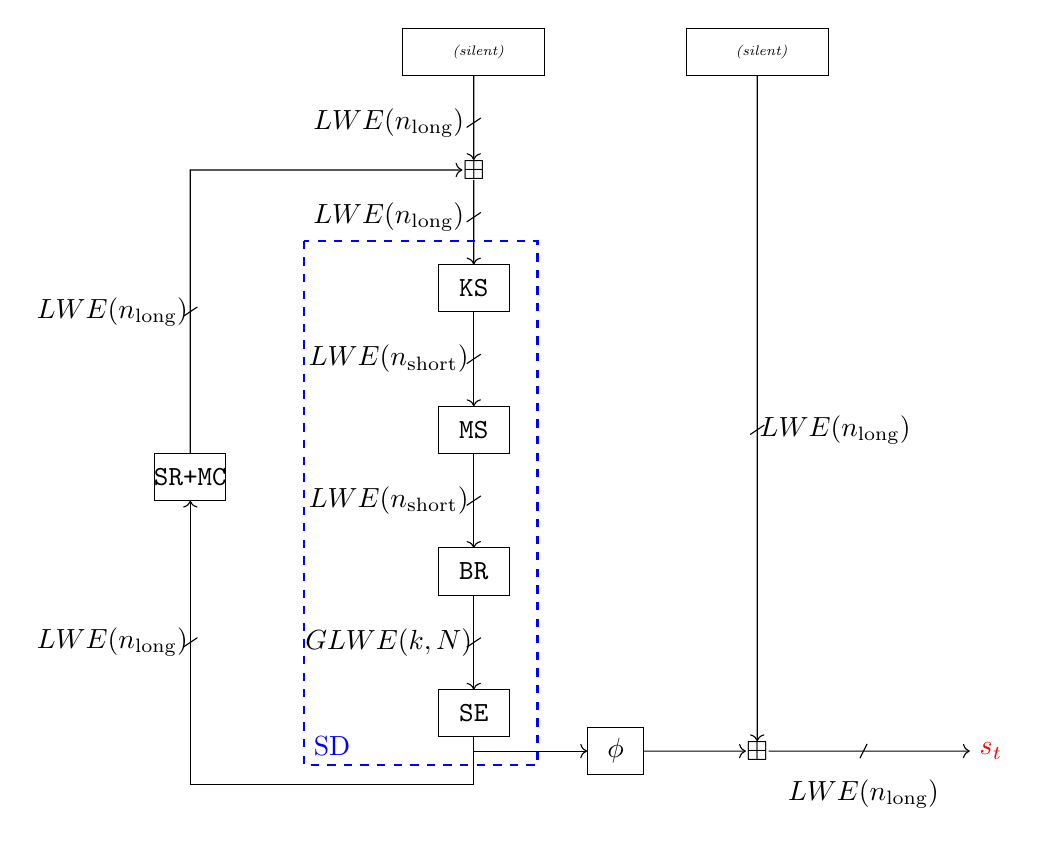
\begin{tikzpicture}[xscale=0.9,yscale=0.6]
 
    %LSFRs
    \draw[] (0, 0) rectangle (2, 1) node[pos=0.5]{$\pseudoKS$ {\tiny \emph{(silent)}}} ;
    \draw[] (4, 0) rectangle (6, 1) node[pos=0.5]{$\whitening$ {\tiny \emph{(silent)}}} ;
    \draw (1, -2) node[inner sep=0pt](addm){$\boxplus$} ;
    \draw[->] (1, 0) -- (addm);

    % FSM
    \draw[] (0.5, -4) rectangle (1.5, -5) node[pos=0.5,color=black](ks){$\texttt{KS}$} ;
    \draw[] (0.5, -7) rectangle (1.5, -8) node[pos=0.5,color=black](ms){$\texttt{MS}$} ;
    \draw[] (0.5, -10) rectangle (1.5, -11) node[pos=0.5,color=black](br){$\texttt{BR}$} ;
    \draw[] (0.5, -13) rectangle (1.5, -14) node[pos=0.5,color=black](se){$\texttt{SE}$} ;
    \draw[] (-3.5, -8) rectangle (-2.5, -9) node[pos=0.5,color=black](srmc){$\texttt{SR+MC}$} ;

    % Draw dashed blue box for SB
    \draw[dashed, blue, thick] (-1.4, -3.5) rectangle (1.9, -14.6);
    \node[blue] at (-1, -14.2) {SD}; % Label for the box

    % FSM connections
    \draw[->] (addm) -- (1, -4);
    \draw[->] (1, -5) -- (1, -7);
    \draw[->] (1, -8) -- (1, -10);
    \draw[->] (1, -11) -- (1, -13);
    \draw[->] (1,-14) -- (1, -15) -- (-3, -15) -- (-3, -9);
    \draw[->] (-3, -8) -- (-3, -2) -- (addm);

    % Extraction
    \draw (5, -14.3) node[inner sep=0pt](addr){$\boxplus$} ;
    \draw[] (2.6, -13.8) rectangle (3.4, -14.8) node[pos=0.5,color=black]{$\phi$} ;

    \draw[->] (1, -14.3) -- (2.6, -14.3);
    \draw[->] (3.4, -14.3) -- (addr);
    \draw[->] (5, 0) -- (addr);
    \draw[->] (addr) -- (8, -14.3);
    \draw[color=red] (8.3, -14.3) node(s){$s_t$} ;



    % Wire type
    \draw (0.9, -1.1) -- (1.1, -0.9) ;
    \draw (-0.2, -1) node{$LWE(n_{\text{long}})$} ;
    \draw (0.9, -3.1) -- (1.1, -2.9) ;
    \draw (-0.2, -3) node{$LWE(n_{\text{long}})$} ;
    \draw (0.9, -6.1) -- (1.1, -5.9) ;
    \draw (-0.2, -6) node{$LWE(n_{\text{short}})$} ;
    \draw (0.9, -9.1) -- (1.1, -8.9) ;
    \draw (-0.2, -9) node{$LWE(n_{\text{short}})$} ;
    \draw (0.9, -12.1) -- (1.1, -11.9) ;
    \draw (-0.2, -12) node{$GLWE(k, N)$} ;
    \draw (-3.1, -12.1) -- (-2.9, -11.9) ;
    \draw (-4.1, -12) node{$LWE(n_{\text{long}})$} ;
    \draw (-3.1, -5.1) -- (-2.9, -4.9) ;
    \draw (-4.1, -5) node{$LWE(n_{\text{long}})$} ;
    \draw (4.9, -7.6) -- (5.1, -7.4) ;
    \draw (6.1, -7.5) node{$LWE(n_{\text{long}})$} ;
    \draw (6.45, -14.45) -- (6.55, -14.15) ;
    \draw (6.5, -15.2) node{$LWE(n_{\text{long}})$} ;

    \end{tikzpicture}
  \vspace{1em}
  \hfill~
  \caption{\label{fig:structure_fhe} Types and shapes of ciphertexts in homomorphic \coolName. The $\subWords$ is broken down into its elementary components}
\end{figure}


% Leo: ce qui suit est pour qu'emacs compile bien l'article, pas touche !
%%% Local Variables:
%%% mode: latex
%%% ispell-local-dictionary: "english"
%%% TeX-master: "../main"
%%% End:




	
}
\fi





\ifeprint{


}
\else{
	\subsection{Concrete Parameters}
	\label{sec:concrete_parameters}
	
	Table \ref{tab:parameters} shows the parameters used for our experiments, all ensuring 128 bits of security. The obtained security levels $\lambda_{\text{short}}$ et $\lambda_{\text{long}}$ have been estimated using the \texttt{lattice estimator}~\cite{lattice-estimator}.
	
	\begin{table}
		\centering
		\caption{TFHE Parameters used in our experimentations}.
			\label{tab:parameters}
		\renewcommand{\arraystretch}{1.3}  % Adjust row spacing
		\scalebox{1}{
			\begin{tabular}{|c||*{12}{>{\centering\arraybackslash}p{0.8cm}|}}
				\hline
				$p_{\text{err}}$ & $q$ & $n_{\text{short}}$ & $k$ & $N$ & $\sigma_{\text{short}}$ & $\sigma_{\text{long}}$ & $B_{BR}$ & $\ell_{\text{BR}}$ & $B_{KS}$ & $\ell_{\text{KS}}$ & $\lambda_{\text{short}}$ & $\lambda_{\text{long}}$\\
				\hline
				$2^{-40}$ & $2^{64}$ & 788 & 2 & 1024 & $2^{47}$ & $2^{14}$ & $2^{23}$ & 1 & $2^4$ & 3 & 131.8 & 128.9\\
				\hline
				$2^{-128}$ & $2^{64}$ & 774 & 1 & 2048 & $2^{47}$ & $2^{14}$ & $2^{23}$ & 1 & $2^3$ & 5 & 131.8 & 128.9\\
				\hline
		\end{tabular}}
		
	\end{table}
}
\fi

\ifeprint{
	
}
\else{
	\subsection{Detailed Homomorphic Implementations}
	\label{sec:detailed_implementation}
	
	In the following, we provide a more detailed way of how we implemented the homomorphic version of \coolName.
	
	\paragraph{Homomorphic evaluation of LSFRs.}
	The \coolName design involves two LSFRs operating on elements of $\field{17}$. The standard way to implement an LSFR is to evaluate the linear feedback function on the state at each clock cycle, thus producing a new element that enters the state, while the state is shifted to output an element. 
	%generate the new element at each clock cycle, and then to mutate the state by shifting the elements of the state and compute the linear combination of the state with the coefficients of retroaction to produce a new one.
	We suggest the \emph{silent LFSR} approach for the homomorphic evaluation of LFSRs. In this approach, the encrypted LFSR state is immutable to avoid any noise growth in the underlying ciphertexts (hence keeping the LFSR ``silent''). We use the fact that every output element of the LFSR can be expressed as a linear combination of the initial state. So, at each clock cycle, we compute \emph{in the clear} the coefficients of this linear combination and homomorphically evaluate it on the immutable encrypted state. This process is depicted in Algorithm~\ref{alg:lsfr}.
	
	\begin{algorithm}[t!]
    \caption{\texttt{LFSR.clock} - Produce a pseudo random element of the state. \label{alg:lsfr}}
    
    \KwIn{
        $\left\{
        \begin{aligned}
            &\ell: \text{ Size of the state of the LFSR.} \\
            &(u_1, \dots, u_\ell): \text{ Encrypted initial state of the LFSR.} \\
            &(\lambda_1^{(0)}, \dots, \lambda_\ell^{(0)}): \text{ Coefficients of retroaction in the definition of the LFSR.} \\
            &(\lambda_1^{(i)}, \dots, \lambda_\ell^{(i)}): \text{ Previous coefficients used in the linear combination.}
        \end{aligned}
        \right.$
    }

    \KwResult{
        $\left\{
        \begin{aligned}
            &o^{(i)}: \text{ Encryption of the $i$-th pseudorandom element of $\F_{17}$.} \\
            &(\lambda_1^{(i+1)}, \dots, \lambda_\ell^{(i+1)}): \text{ Updated coefficients of the linear combination.}
        \end{aligned}
        \right.$
    }

    % Add vertical space and horizontal line
    \vspace{0.5em} % adjust the space as needed
    \hrule
    \vspace{0.5em} % adjust the space as needed

    $o^{(i)} \gets 0$

    \Comment{Evaluation of the linear combination}
    \For{$k \in \{1, \dots, \ell\}$}{
        $o^{(i)} \gets \texttt{SumTFHE}(o^{(i)}, \texttt{ClearMultTFHE}(u_k, \lambda_k^{(i)}))$
    }
    \Comment{Update of the next coefficients}
    \For{$k \in \{2, \dots, \ell\}$}{
        $\lambda_k^{(i+1)} \gets \lambda_{k-1}^{(i)} + \lambda_\ell^{(i)} \cdot \lambda_k^{(0)}$
    }
    $\lambda_1^{(i+1)} \gets \lambda_\ell^{(i)} \cdot \lambda_1^{(0)}$
    
    \Return{$o^{(i)}$}
    
\end{algorithm}


	
	%Calling Algorithm \ref{alg:lsfr} (\texttt{LFSR.clock}) several times yields an encrypted stream of pseudorandom elements $(o^{(0)}, o^{(1)}, \dots)$.
	
	\paragraph{Homomorphic evaluation of} \coolName. The complete homomorphic evaluation of a round of one clock cycle of \coolName is depicted in Algorithm~\ref{alg:transistor}, using $\pseudoKS.\texttt{clock}$ and $\whitening.\texttt{clock}$ as subroutines (i.e., Algorithm~\ref{alg:lsfr} evaluated on the key schedule and whitening LFSRs). The most computation intensive part of the algorithm is by far the evaluation of the PBS in $\subWords$ which can be fully parallelized to reduce the latency.
	
	\begin{algorithm}[t!]
    \caption{\texttt{Transistor.clock} - Produce $r$ encypted elements of the key stream}
    \label{alg:transistor}
    
 
    \KwIn{
        $\left\{
        \begin{aligned}
        	&\mathcal K: \text{the LFSR used for the pseudo-keyschedule and its state (cf Algorithm \ref{alg:lsfr}).}\\
            &\mathcal W: \text{the LFSR used for the whitening.}\\	
            &X = \left ( \begin{array}{ccc}
            x_{1,1} & \dots & x_{1,\sqrt{m}}\\
            \dots & \dots & \dots\\
            x_{\sqrt{m},1} & \dots & x_{\sqrt{m},\sqrt{m}}\\
            \end{array} \right ): \text{ Encrypted state of the FSM} \\
        \end{aligned}
        \right.$
    }

    \KwResult{
        $\left\{
        \begin{aligned}
            &Y = (y_1, \dots, y_r): \text{ Encryption of $r$ elements of the  key stream } \\
        \end{aligned}
        \right.$
    }

    % Add vertical space and horizontal line
    \vspace{0.5em} % adjust the space as needed
    \hrule
    \vspace{0.5em} % adjust the space as needed

    \Comment{Compute the pseudo-key schedule and adds it to the FSM}
    \For{$i \in [1, \sqrt m]$}{
        \For{$j \in [1, \sqrt m]$}{
            $k_{i,j} \gets \pseudoKS.\texttt{clock}()$\\
            $x_{i,j} \gets \texttt{SumTFHE}(x_{ij}, k_{i,j})$\\
        }
    }
    \Comment{Compute $\subWords$ with a layer of PBS}
    \For{$i \in [1, \sqrt m]$}{
        \For{$j \in [1, \sqrt m]$}{        
            $x_{i,j} \gets \texttt{PBS\_TFHE}(x_{i,j}, S)$\\
        }
    }
    \Comment{Extract the output bits and whiten them}
    $(y_1, \dots, y_r) \gets \phi(X)$\\
    \For{$i \in [1, r]$}{
        $w_i \gets \whitening.\texttt{clock}()$\\
        $y_i \gets \texttt{SumTFHE}(y_i, w_i)$\\
    }
    \Comment{Compute $\shiftRows$, (same as in clear)}
    $X \gets \shiftR(X)$

    \Comment{Compute MixColumns}
    \For{$i \in [1, \sqrt m]$}{
        \For{$j \in [1, \sqrt m]$}{
            $z_{i, j} \gets 0$\\
            \For{$k \in [1, \sqrt m]$}{
                $z_{i, j} \gets \texttt{SumTFHE}(z_{i, j}, \texttt{ClearMultTFHE}(x_{k, j}, MC_{i, k}))$\\
            }
        }
    }

    \Return{$Y$}

\end{algorithm}


	}
\fi

\ifeprint{

}
\else{
	\subsection{Size of the server key}
	\label{sec:server_key_sizes}
	We  provide the sizes for the server keys in Table \ref{tab:server_key_size}, namely the \emph{key-switching key} (KSK) and the \emph{bootstrapping key} (BSK) while using the ciphertext compression technique described in Section~\ref{sec:key_wrapping}. Those keys are only generated and communicated to the server once (during some user enrolment step).
	
	
	
	\begin{table}
		\centering
		\caption{Size of the server keys for the two considered sets of parameters. 
			%This is agnostic to the volume of message sent. 
			\label{tab:server_key_size}}
		
		\renewcommand{\arraystretch}{1.2}  % Adjust row spacing
		\scalebox{0.9}{
			\begin{tabular}{|c||*{3}{>{\centering\arraybackslash}p{4cm}|}}
				\hline
				& Theoretical sizes & Sizes for $p_{\text{err}} = 2^{-40}$ & Sizes for $p_{\text{err}} = 2^{-128}$ \\
				\hline
				~KSK~ &  $n_{\text{long}}\cdot l_{\text{KS}} \cdot \log_2 q $ & 49 KB & 82 KB  \\
				\hline
				~BSK~ &  $n_{\text{short}} \cdot l_{\text{BS}} \cdot \log_2 q \cdot N \cdot (k+1)$ & 6.5 MB & 12.7 MB  \\
				\hline
		\end{tabular}}
		
	\end{table}
}
\fi



%% !TeX root = ./main.tex
\section{Additionnal Cryptanalysis}
\label{sec:appendix-cryptanalysis}



\subsection{Algebraic Analysis}
\label{sec:cryptanalysis-algebraic}
Algebraic cryptanalysis consists of formulating nonlinear equations that an attacker can derive from the information observed in terms of the secret key material. Several techniques, such as Gröbner basis methods or linearization, exist for solving such systems of equations, and we discuss them in this section. Based on this analysis, we claim that \coolName{} is resistant to algebraic attacks and their improvements.

%A first generic approach can be to rely on a Gröbner basis. A second generic approach can be to use linearization technique, that is considering any multivariate monomial involved in the system as new and independent variable also be to and a second approach to attacks based on deriving low-degree equations in the internal state from the observation of the keystream. We also discuss linearization techniques further below.


\paragraph{Gröbner Basis.} Such an attack consists of four main steps: formulating the equations that model the intended cryptanalysis, computing their Gröbner basis, applying a ``change of monomial ordering'' to transform the Gröbner basis into a more useful form, and finally solving the result using univariate techniques. The complexity of the first and last steps is usually negligible, meaning that we should evaluate the time complexity of at least one of the other two steps.

However, as recently shown in~\cite{C:BBLAOP24}, it is possible to write the equations in such a way as to entirely bypass the computation of the Gröbner basis. This is achieved by choosing a custom \emph{monomial ordering} that ensures the equations, as formulated, immediately form a Gröbner basis. This approach can be applied here by assigning increasing weights to the successive outputs of the key schedule, so that the leading monomials in each equation involve only a single key variable. This method is effective for at least the first four clock cycles, as the clock outputs are independent.

At this stage, we have 16 independent equations of degree 15 (the degree of $\thesbox$). Adding the equations corresponding to the next $20$ clocks, we get as many equations as unknowns, which, in particular, should lead to a 0-dimensional ideal. As conjectured in~\cite{EPRINT:Perrin24}, the ideal degree of this system can be lower-bounded by $15^{16} \approx 2^{62.5}$. This bound would be exact if the 80 remaining equations somehow failed to contribute to an increase in this quantity, or if the ideal degree was in some way decreased by one of these equations (despite the 0-dimension). Given that change of order algorithms are at least quadratic in the ideal degree, we can safely claim security against Gröbner-basis-based algebraic attacks.

%\paragraph{Classical Algebraic Attack.} \lp{todo. On dit qu'on s'en fout parce que faire 0 dans $\mainField$ ça dit pas grand chose?}\yr{Oui, on s'en fout}


\paragraph{Linearization.}Such attacks may, a priori, pose a threat, as they have led to the downfall of two \gls{FHE}-friendly stream ciphers, namely {\tt FLIP}~\cite{EC:MJSC16} and {\tt Elisabeth}~\cite{AC:CHMS22}, which were broken in~\cite{C:DuvLalRot16} and~\cite{AC:GBJR23}, respectively. The structure of these ciphers made such attacks an inherent risk: in both cases, a low-degree function is applied to a constant key register to generate keystream words.  As a result, in these ciphers, the nonlinear equations derived from the keystream sequence have a constant degree. Considering all monomials (or linear combinations of monomials) as new independent variables in this representation enables powerful attacks~\cite{C:DuvLalRot16,AC:GBJR23}. These attacks are the result of  two fundamental weaknesses: the constant degree of the system and low diffusion, as the registers are never updated, only a bit-permutation is applied at each clock cycle.

These issues are directly addressed in the design of \coolName{}. First, the round function of the FSM applies the S-box \( \thesbox \) to every digit. This S-box has a univariate representation in \( \mainField \) that is both dense and of degree 15. Furthermore, the content of the FSM accumulates high-degree equations within the key-LFSR. As a result, the multivariate polynomial representation of the keystream digits will not have a constant degree; instead, it will be very dense and of high degree.


\paragraph{Using Annihilators.} Another powerful technique is to directly use an annihilator of the filtering function, where this annihilator has a lower degree than the original function~\cite{EC:CouMei03,C:Courtois03}. This allows the attacker to collect and solve a system of equations with a smaller degree than the original one. That is, similar to Gröbner basis-like attacks, this approach operates on the ideal generated by the polynomials. In the case of \coolName{}, we can argue and defend the role of the whitening LFSR \( \whitening \). Indeed, this LFSR has a length of 32 digits, meaning that an annihilator at the output must consider the sum of 8 outputs by \( \phi \) and cancel them with a polynomial. Therefore, without additional information, such an annihilator would need to multiply approximately 32 digits, leading to an increase in the degree. This strategy must also account for the degree increase in successive outputs of \( \phi \), as discussed above.

\paragraph{Other Techniques.}
Last but not least, algebraic attacks can be improved in several ways using the Guess-and-Determine strategy or the so-called Hybrid approach in Gröbner basis computations. In our case, one could guess key-register cells, whitening-key cells, or cells in the FSM. Although this is a valid approach, the remaining equations (depending on the guessing strategy) would either have an increased degree or require guessing too many cells, making the attack impractical.



\subsection{Comparison With {\tt LEX}}
\label{sec:security-lex}

{\tt LEX}~\cite{SAC:Biryukov06} is a stream cipher designed by Biryukov in 2006 and selected to the third phase of the eSTREAM competition. {\tt LEX} employed a rather unusual design for a stream cipher, based on the {\tt \gls{AES}} block cipher and a technique called \emph{leak extraction}. The idea of the leak extraction is to produce the key stream by extracting parts of the underlying block cipher state.

The description of {\tt LEX} is very simple and elegant. It is based on a slightly tweaked version of the {\tt \gls{AES}} where the {\sf AddRoundKey} operation before the first round is omitted and where the {\tt MixColumns} of the last round is not. For simplicity, we will still refer to this tweaked version as {\tt \gls{AES}}. First, the publicly known $IV$ is encrypted by the {\tt \gls{AES}} under the secret key $K$ to produce an initial state  $S = {\tt \gls{AES}}_K(IV)$. Then, the state $S$ is repeatedly encrypted using the OFB mode and the same secret key $K$. At each round of encryption, four words of the internal state are extracted to compose the key stream produced by {\tt LEX}. The positions of the extracted words depend on the round number and are depicted in Figure~\ref{fig:lex}.

\begin{figure}
  \centering
  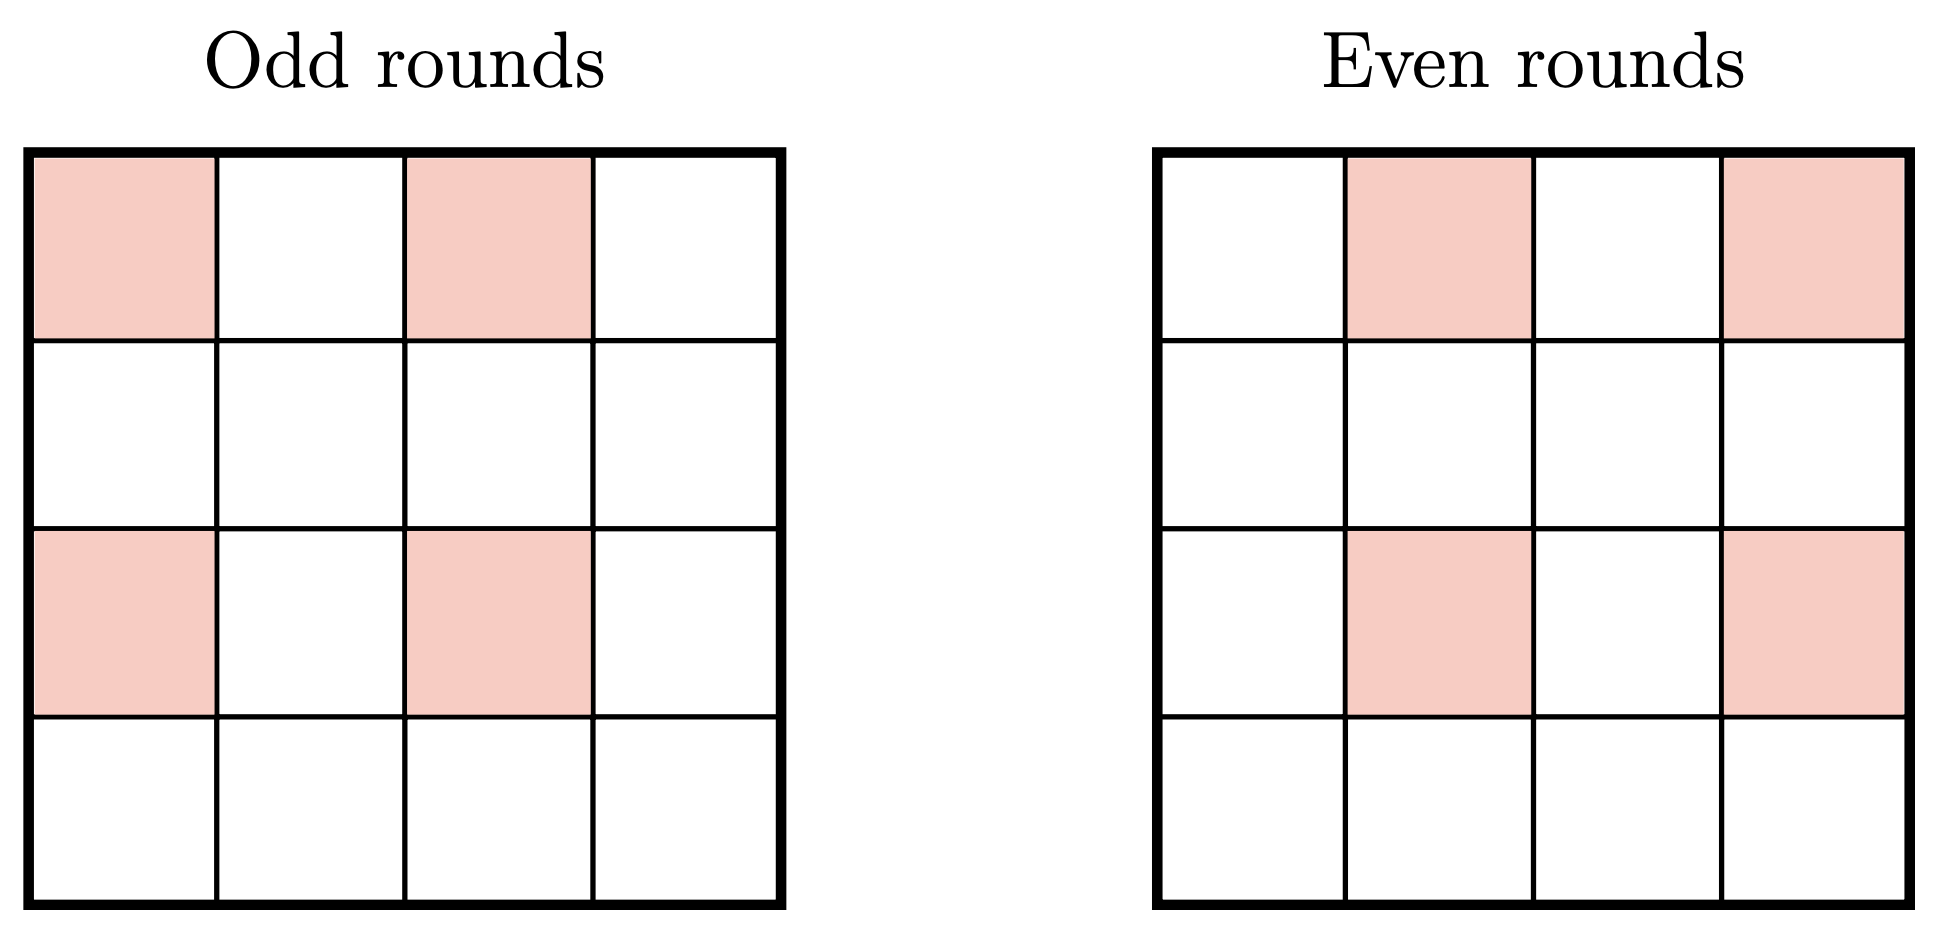
\includegraphics[width=7cm]{figures/lex.png}
  \caption{Extraction of internal state words for odd and even rounds of {\tt LEX}\label{fig:lex}. The extracted words are the ones being colored.}
\end{figure}

In 2008, Dunkelman and Keller presented an attack against LEX~\cite{AC:DunKel08b} able to recover the 128-bit secret key with $2^{36.3}$ bytes of key-stream produced by the same key and a time complexity of $2^{112}$ simple operations. This attack worked by exploiting a particular difference pattern of probability $2^{-64}$ in the {\tt \gls{AES}} internal state that could be detected by observing a $32$-bit condition in the output key stream.  The attack can be decomposed  in the three following steps:
\begin{enumerate}
\item  The attacker observes the output stream for a specific 32-bit pattern to occur (the four output words at a certain round should all be zero). This potentially indicates a special difference pattern (8 particular words with zero-difference) in the internal state of {\tt \gls{AES}}. 
\item Once this difference pattern is detected, the attacker recovers the values of 16 bytes of the internal state in both {\tt \gls{AES}} encryptions. This is achieved by guessing the difference in eight additional state words and by exploiting simple properties of the  {\sf MixColumns} and the  S-box. 
\item Finally, using the recovered 16 bytes, the attacker proceeds with a guess-and-determine approach to retrieve the secret key. The key step here is exploiting relations derived from the {\tt \gls{AES}-128} key schedule that link bytes from three consecutive subkeys, reducing the number of required guesses to just two subkey bytes. This limits the guessing process to only 10 bytes (80 bits) in total.
\end{enumerate}

\coolName{}'s structure ressembles {\tt LEX} in several aspects, the most notable being the extraction of four words at each iteration. Additionally, \coolName{}'s round function is inspired by the {\tt \gls{AES}} round function. For these reasons, it is natural to question whether the attack described in~\cite{AC:DunKel08b} could be adapted to \coolName{}. However, as we will argue next,  \coolName{} differs from {\tt LEX} in some crucial design choices, making the Dunkelman and Keller attack very difficult to apply:

\begin{itemize}
\item The output of the FSM at every round is masked by the whitening LFSR $\mathcal{W}$ making it hard to directly recover the values of the internal state as done in the attack of {\tt LEX}.
\item The LFSR $\mathcal{K}$ playing the role of the key schedule, produces uncorrelated outputs, making it hard to find simple relations between key values in consecutive rounds. A crucial element in the success of the attack against {\tt LEX} was exactly the fact that by guessing only two key bytes, the attacker was able to recover many more key values by exploiting such relations holding over several rounds. As we showed in the previous sections, it is not possible for an attacker to extract any information on the secret key by observing the output of the FSM over 3 or 4 consecutive rounds. 
\end{itemize}


\subsection{Truncated Linear Trails from MILP}
\label{sec:milp}


In order to find a lower bound for the number of S-boxes active in a linear trail over 4 rounds of \coolName, we apply the approach introduced by Mouha \emph{et al.\@}~\cite{add:MWGP11} in the most direct way. As we are interested in the (in)activity of the Sboxes throughout the rounds, we only need to assign binary variables to output digits, but also to internal digits of the state before the S-box layer, and before the MixColumn operation. For each round, we then have $4 + 16 + 16 = 36$ binary variables that are related one to others by the following constraints.
\begin{description}
\item[3-fork constraint.] Any output digit corresponds to a digit of the internal state after the S-box layer, so it is naturally related to the activity of a digit before MixColumn, by taking care of the reorganization of the digits through ShiftRows. But because the activity pattern is unchanged through the S-box layer, it is also related to a digit before the S-box layer. The constraint between three such variables is that if one is active, then at least two of them are. This corresponds to a 3-fork constraint that can be modeled as in \cite[Sec~ 2.2]{add:MWGP11}.
\item[MDS constraint.] A given column before and after MixColumns are related by the following MDS constraint: if a digit is active, then at least 5 of them are. This can be modeled in a manner similar to the 3-fork. In our case, the binary variables associated to the state after MixColumns at round $r$ are the one corresponding to the state before the S-box layer at round $r+1$.
\item[Border constraints.] We also add some border constraints to ensure that the initial inner state is fully inactive, and that the same holds for the final inner state. This way, we make sure that the considered linear equations do not depend on the unknown FSM state, but only on the key and output digits. We also impose that at least a digit among the ones output at the first round, and at least one among the ones of the last round must be active.
\end{description}
Finally, with the described constraints, the objective is to minimize the number of active Sboxes, that is, the number of active digits before the S-box layer. Note that any solution to this problem is actually a worst-case scenario in our case: a returned activation pattern is not guaranteed to be actually instantiable. We solved this simple MILP model using the SageMath interface for Mixed Integer Linear Programing solving within seconds on a standard laptop. Our code is 
\ifeprint
  available online.\footnote{\url{https://github.com/CryptoExperts/Transistor/}}
\else
  provided as supplementary material.
\fi

Most notably, we have found that
\[w_4 \geq 13,\  w_5 \geq 20 \mbox{ and } w_6 \geq 25\]
with the potential trail examples depicted on Fig.~\ref{fig:trails}.
We also verified that \(w_n \geq 26\) for $n \in \{7, 8, \ldots 26\}$.
For larger values of $n$, either a trail has at least one active S-box per
round, or it splits into two smaller trails with at least 13 active
Sboxes.  Therefore, we deduce that \(w_n \ge 26\) for all $n \ge 7$.

\begin{figure}[h]
  \centering
  \begin{subfigure}[t]{0.22\textwidth}
    \centering
    \includegraphics[scale=.55]{figures/solution_0.pdf}
    \caption{4-round trail.}
  \end{subfigure}
  \hfill
  \begin{subfigure}[t]{0.22\textwidth}
    \centering
    \includegraphics[scale=.55]{figures/solution_1.pdf}
    \caption{4-round trail.}
  \end{subfigure}
  \hfill
  \begin{subfigure}[t]{0.22\textwidth}
    \centering
    \includegraphics[scale=.55]{figures/solution_2.pdf}
    \caption{4-round trail.}
  \end{subfigure}
  \hfill
  \begin{subfigure}[t]{0.22\textwidth}
    \centering
    \includegraphics[scale=.55]{figures/solution_3.pdf}
    \caption{4-round trail.}
  \end{subfigure}
  
  \begin{subfigure}[t]{0.45\textwidth}
    \centering
    \includegraphics[scale=.6]{figures/milp_5.pdf}
    \caption{5-round trail.}
  \end{subfigure}
  \caption{Activity patterns for linear trails over 4 and 5 rounds.}
  \label{fig:trails}
\end{figure}

%\ac{Donner les figures des 4 trails tronques pour \(4\) tours ici.}


% Leo: ce qui suit est pour qu'emacs compile bien l'article, pas touche !
%%% Local Variables:
%%% mode: latex
%%% ispell-local-dictionary: "english"
%%% TeX-master: "main"
%%% End:




\chapter{Accelerating Large Look-Up Tables}
\label{chap:larger_lut}
\input{tex/larger_luts/main_larger_luts.tex}


\chapter{A Practical Solution for Parameter Selection}
\label{chap:parameters}
\input{tex/orpheus/main_orpheus.tex}


\chapter*{Conclusion}
\addstarredchapter{Conclusion}

Fully Homomorphic Encryption is believed to be on the verge of practical usability. But still some challenges are remaining so it can be used in our day-to-day life. In the following, we show how the works presented in this thesis adresses in these issues.

The purpose of this thesis was to adress some concrete obstacles that hinder the practical deployment of \gls{FHE}. In this concluding section, we list the main challenges and relate them to the contributions presented throughout this manuscript.

\paragraph{On Efficiency.}

\gls{FHE} still incurs an significant computational overhead compared to traditional, unencrypted computation. While the \gls{FHE} schemes themselves have been seen much improvement in the last years, an orthogonal direction is to design new algorithms tailored for specific use-cases. In Chapter \ref{chap:p_encodings}, we developed a framework to accelerate the evaluation of Boolean functions. At the opposite end of the spectrum, Chapter \ref{chap:larger_lut} focus on accelerating the evaluation of \gls{LUT} in larger plaintext spaces than those originally supported by \gls{TFHE}. Chapter \ref{chap:hyppogriph} further demonstrated how Boolean and arithmetic representations offer complementary advantages, and how efficient conversion mechanisms between both can enhance performance within homomorphic circuits. 

Another way of improving performances lies in selecting appropriate parameters for the scheme. We propose such a procedure of parameter selection, which takes into account the computational circuit to evaluate as well as the environment of execution.


\paragraph{On Data Expansion and Transciphering.}


Data expansion is another well-known bottleneck in \gls{FHE}. The literature has long proposed transciphering as a promising solution, however this technique necessitates homomorphic evaluation of the decryption function of a symmetric cipher. In Chapter \ref{chap:hyppogriph}, we have shown how far we could push to evaluate efficiently the \gls{AES} cipher using \gls{TFHE}. However, it is clear that standard ciphers such as \gls{AES} cannot compete against schemes specifically designed with the use-case of transciphering in mind. In Chapter \ref{chap:transistor}, we present such a cipher and show how its design combines the properties required to ensure both cryptographic security and homomorphic efficiency. 




\paragraph{On Compilation and Development of Homomorphic Computations.}
%

Developing homomorphic applications remains a tedious task, requiring deep understanding of both cryptography and the internal workings of specific \gls{FHE} schemes. It is clear that an adoption of \gls{FHE} at scale will require an automated compilation toolchain that will abstract away cryptography complexities from non-expert programmers.

In Chapter \ref{chap:p_encodings}, we proposed algorithm that automatically compiles Boolean functions into optimized sequences of homomorphic operations. We did a similar thing in the case of large LUTs in Chapter \ref{chap:larger_lut}, where those LUTs are compiled into a more tractable algorithm, composed of smaller ones. Finally, our parameter selection framework presented in \ref{chap:parameters} further contributes to this effort.


\bigskip

The road is probably still long until \gls{FHE} becomes an ubiquitous technology. But the pace of scientific progress in this field is accelerating rapidly. So it is reasonable to believe (and hope) that such a technological revolution will happen in a not-so-distant future.







\printbibliography



\appendix
\chapter{Supplementary Material on Parameter Selection}
\input{tex/orpheus/appendix_example_cjp.tex}


% =============================================
%                 END
% =============================================




%==============================
\end{document}